% Options for packages loaded elsewhere
\PassOptionsToPackage{unicode}{hyperref}
\PassOptionsToPackage{hyphens}{url}
%
\documentclass[
]{book}
\usepackage{amsmath,amssymb}
\usepackage{iftex}
\ifPDFTeX
  \usepackage[T1]{fontenc}
  \usepackage[utf8]{inputenc}
  \usepackage{textcomp} % provide euro and other symbols
\else % if luatex or xetex
  \usepackage{unicode-math} % this also loads fontspec
  \defaultfontfeatures{Scale=MatchLowercase}
  \defaultfontfeatures[\rmfamily]{Ligatures=TeX,Scale=1}
\fi
\usepackage{lmodern}
\ifPDFTeX\else
  % xetex/luatex font selection
\fi
% Use upquote if available, for straight quotes in verbatim environments
\IfFileExists{upquote.sty}{\usepackage{upquote}}{}
\IfFileExists{microtype.sty}{% use microtype if available
  \usepackage[]{microtype}
  \UseMicrotypeSet[protrusion]{basicmath} % disable protrusion for tt fonts
}{}
\makeatletter
\@ifundefined{KOMAClassName}{% if non-KOMA class
  \IfFileExists{parskip.sty}{%
    \usepackage{parskip}
  }{% else
    \setlength{\parindent}{0pt}
    \setlength{\parskip}{6pt plus 2pt minus 1pt}}
}{% if KOMA class
  \KOMAoptions{parskip=half}}
\makeatother
\usepackage{xcolor}
\usepackage{color}
\usepackage{fancyvrb}
\newcommand{\VerbBar}{|}
\newcommand{\VERB}{\Verb[commandchars=\\\{\}]}
\DefineVerbatimEnvironment{Highlighting}{Verbatim}{commandchars=\\\{\}}
% Add ',fontsize=\small' for more characters per line
\usepackage{framed}
\definecolor{shadecolor}{RGB}{248,248,248}
\newenvironment{Shaded}{\begin{snugshade}}{\end{snugshade}}
\newcommand{\AlertTok}[1]{\textcolor[rgb]{0.94,0.16,0.16}{#1}}
\newcommand{\AnnotationTok}[1]{\textcolor[rgb]{0.56,0.35,0.01}{\textbf{\textit{#1}}}}
\newcommand{\AttributeTok}[1]{\textcolor[rgb]{0.13,0.29,0.53}{#1}}
\newcommand{\BaseNTok}[1]{\textcolor[rgb]{0.00,0.00,0.81}{#1}}
\newcommand{\BuiltInTok}[1]{#1}
\newcommand{\CharTok}[1]{\textcolor[rgb]{0.31,0.60,0.02}{#1}}
\newcommand{\CommentTok}[1]{\textcolor[rgb]{0.56,0.35,0.01}{\textit{#1}}}
\newcommand{\CommentVarTok}[1]{\textcolor[rgb]{0.56,0.35,0.01}{\textbf{\textit{#1}}}}
\newcommand{\ConstantTok}[1]{\textcolor[rgb]{0.56,0.35,0.01}{#1}}
\newcommand{\ControlFlowTok}[1]{\textcolor[rgb]{0.13,0.29,0.53}{\textbf{#1}}}
\newcommand{\DataTypeTok}[1]{\textcolor[rgb]{0.13,0.29,0.53}{#1}}
\newcommand{\DecValTok}[1]{\textcolor[rgb]{0.00,0.00,0.81}{#1}}
\newcommand{\DocumentationTok}[1]{\textcolor[rgb]{0.56,0.35,0.01}{\textbf{\textit{#1}}}}
\newcommand{\ErrorTok}[1]{\textcolor[rgb]{0.64,0.00,0.00}{\textbf{#1}}}
\newcommand{\ExtensionTok}[1]{#1}
\newcommand{\FloatTok}[1]{\textcolor[rgb]{0.00,0.00,0.81}{#1}}
\newcommand{\FunctionTok}[1]{\textcolor[rgb]{0.13,0.29,0.53}{\textbf{#1}}}
\newcommand{\ImportTok}[1]{#1}
\newcommand{\InformationTok}[1]{\textcolor[rgb]{0.56,0.35,0.01}{\textbf{\textit{#1}}}}
\newcommand{\KeywordTok}[1]{\textcolor[rgb]{0.13,0.29,0.53}{\textbf{#1}}}
\newcommand{\NormalTok}[1]{#1}
\newcommand{\OperatorTok}[1]{\textcolor[rgb]{0.81,0.36,0.00}{\textbf{#1}}}
\newcommand{\OtherTok}[1]{\textcolor[rgb]{0.56,0.35,0.01}{#1}}
\newcommand{\PreprocessorTok}[1]{\textcolor[rgb]{0.56,0.35,0.01}{\textit{#1}}}
\newcommand{\RegionMarkerTok}[1]{#1}
\newcommand{\SpecialCharTok}[1]{\textcolor[rgb]{0.81,0.36,0.00}{\textbf{#1}}}
\newcommand{\SpecialStringTok}[1]{\textcolor[rgb]{0.31,0.60,0.02}{#1}}
\newcommand{\StringTok}[1]{\textcolor[rgb]{0.31,0.60,0.02}{#1}}
\newcommand{\VariableTok}[1]{\textcolor[rgb]{0.00,0.00,0.00}{#1}}
\newcommand{\VerbatimStringTok}[1]{\textcolor[rgb]{0.31,0.60,0.02}{#1}}
\newcommand{\WarningTok}[1]{\textcolor[rgb]{0.56,0.35,0.01}{\textbf{\textit{#1}}}}
\usepackage{longtable,booktabs,array}
\usepackage{calc} % for calculating minipage widths
% Correct order of tables after \paragraph or \subparagraph
\usepackage{etoolbox}
\makeatletter
\patchcmd\longtable{\par}{\if@noskipsec\mbox{}\fi\par}{}{}
\makeatother
% Allow footnotes in longtable head/foot
\IfFileExists{footnotehyper.sty}{\usepackage{footnotehyper}}{\usepackage{footnote}}
\makesavenoteenv{longtable}
\usepackage{graphicx}
\makeatletter
\def\maxwidth{\ifdim\Gin@nat@width>\linewidth\linewidth\else\Gin@nat@width\fi}
\def\maxheight{\ifdim\Gin@nat@height>\textheight\textheight\else\Gin@nat@height\fi}
\makeatother
% Scale images if necessary, so that they will not overflow the page
% margins by default, and it is still possible to overwrite the defaults
% using explicit options in \includegraphics[width, height, ...]{}
\setkeys{Gin}{width=\maxwidth,height=\maxheight,keepaspectratio}
% Set default figure placement to htbp
\makeatletter
\def\fps@figure{htbp}
\makeatother
\setlength{\emergencystretch}{3em} % prevent overfull lines
\providecommand{\tightlist}{%
  \setlength{\itemsep}{0pt}\setlength{\parskip}{0pt}}
\setcounter{secnumdepth}{5}
\usepackage{booktabs}
\usepackage{amsthm}
\makeatletter
\def\thm@space@setup{%
  \thm@preskip=8pt plus 2pt minus 4pt
  \thm@postskip=\thm@preskip
}
\makeatother
\ifLuaTeX
  \usepackage{selnolig}  % disable illegal ligatures
\fi
\usepackage[]{natbib}
\bibliographystyle{apalike}
\usepackage{bookmark}
\IfFileExists{xurl.sty}{\usepackage{xurl}}{} % add URL line breaks if available
\urlstyle{same}
\hypersetup{
  pdftitle={Understanding Uncertainty Course Notes},
  pdfauthor={Jeffrey Woo},
  hidelinks,
  pdfcreator={LaTeX via pandoc}}

\title{Understanding Uncertainty Course Notes}
\author{Jeffrey Woo}
\date{2025-07-30}

\begin{document}
\maketitle

{
\setcounter{tocdepth}{1}
\tableofcontents
}
\chapter*{Preface}\label{preface}
\addcontentsline{toc}{chapter}{Preface}

The examples in this preface is based on OpenIntro Statistics (Diez, Ceytinka-Rundel, Barr), Chapter 9.4 and 9.5, which provide more background information. You can access the book for free at \url{https://www.openintro.org/book/os/}

The main goal using data science is to understand data. Broadly speaking, this will involve building a statistical model for predicting, or estimating a response variable based on one or more predictors. Such models are used in a wide variety of fields such as finance, medicine, public policy, sports, and so on. We will look a couple of examples.

\section{Examples}\label{examples}

\subsection{Example 1: Mario Kart Auction Prices}\label{example-1-mario-kart-auction-prices}

In this first example, we will look at Ebay auctions of a video game called Mario Kart that is played on Nintendo Wii. We want to predict the price of an auction based on whether the game is new or not, whether the auction's main photo is a stock photo, the duration of the auction in days, and the number of Wii wheels included with the auction.

A model that we can use for this example is the linear regression model:

\begin{Shaded}
\begin{Highlighting}[]
\FunctionTok{library}\NormalTok{(openintro)}

\NormalTok{Data}\OtherTok{\textless{}{-}}\NormalTok{mariokart}
\DocumentationTok{\#\#fit model}
\NormalTok{result}\OtherTok{\textless{}{-}}\FunctionTok{lm}\NormalTok{(total\_pr}\SpecialCharTok{\textasciitilde{}}\NormalTok{cond}\SpecialCharTok{+}\NormalTok{stock\_photo}\SpecialCharTok{+}\NormalTok{duration}\SpecialCharTok{+}\NormalTok{wheels, }\AttributeTok{data=}\NormalTok{Data)}
\end{Highlighting}
\end{Shaded}

Generally speaking, a linear regression equation takes the following form:

\[
\hat{y} = \hat{\beta}_0 + \hat{\beta}_1 x_1 + \hat{\beta}_2 x_2 + \cdots + \hat{\beta}_k x_k
\]

where \(\hat{y}\) denotes the predicted value of the response variable, the price of the action in this example, \(x_1, x_2, \cdots, x_k\) denote the values of the predictors. This is example, we have: \(x_1\) for whether the game is new or not, \(x_2\) for whether the auction's main photo is a stock photo, \(x_3\) for the duration of the auction in days, and \(x_4\) for the number of Wii wheels included with the auction. \(\hat{\beta}_0, \hat{\beta}_1, \cdots, \hat{\beta}_k\) represent the estimated regression parameters. If we know what these values are, we can easily plug in the values of the predictors to obtain the predicted price of the auction.

Fitting the model in R, we obtain the estimated regression parameters:

\begin{Shaded}
\begin{Highlighting}[]
\DocumentationTok{\#\#get estimated regression parameters}
\NormalTok{result}
\end{Highlighting}
\end{Shaded}

\begin{verbatim}
## 
## Call:
## lm(formula = total_pr ~ cond + stock_photo + duration + wheels, 
##     data = Data)
## 
## Coefficients:
##    (Intercept)        condused  stock_photoyes        duration          wheels  
##        43.5201         -2.5816         -6.7542          0.3788          9.9476
\end{verbatim}

so we have:

\[
\hat{y} = 43.5201 - 2.5816 x_1 - 6.7542 x_2 + 0.3788 x_3 + 9.9476 x_4
\]

So for an auction for Mario Kart game that is used, that uses a stock photo, is listed for 2 days, and comes with 0 wheels, the predicted price will be \(\hat{y} = 43.5201 - 2.5816 - 6.7542 + 0.3788 \times 2 = 34.94\) or about 35 dollars.

\subsection{Example 2: Job Application Callback Rates}\label{eg2}

In this example, we look at data from an experiment that sought to evaluate the effect of race and gender on job application callback rates. For the experiment, researchers created fake resumes to job postings in Boston and Chicago to see which resumes resulted in a callback. The fake resumes included relevant information such as the applicant's educational attainment, how many year's of experience the applicant as well as a first and last name. The names on the fake resume were meant to imply the applicant's race and gender. Only two races were considered (Black or White) and only two genders were considered (Make or Female) for the experiment.

Prior to the experiment, the researchers conducted surveys to check for racial and gender associations for the names on the fake resumes; only names that passed a certain threshold from the surveys were included in the experiment.

A model that can be used in this example is the logistic regression model

\begin{Shaded}
\begin{Highlighting}[]
\NormalTok{Data2}\OtherTok{\textless{}{-}}\NormalTok{resume}
\DocumentationTok{\#\#fit model}
\NormalTok{result2}\OtherTok{\textless{}{-}}\FunctionTok{glm}\NormalTok{(received\_callback}\SpecialCharTok{\textasciitilde{}}\NormalTok{job\_city }\SpecialCharTok{+}\NormalTok{ college\_degree}\SpecialCharTok{+}\NormalTok{years\_experience}\SpecialCharTok{+}\NormalTok{race}\SpecialCharTok{+}\NormalTok{gender, }\AttributeTok{family=}\StringTok{"binomial"}\NormalTok{, }\AttributeTok{data=}\NormalTok{Data2)}
\end{Highlighting}
\end{Shaded}

Generally speaking, a logistic regression equation takes the following form

\[
\log (\frac{\hat{\pi}}{1-\hat{\pi}}) = \hat{\beta}_0 + \hat{\beta}_1 x_1 + \hat{\beta}_2 x_2 + \cdots + \hat{\beta}_k x_k
\]

where \(\hat{\pi}\) denotes the predicted probability that the applicant receives a call back. \(x_1, x_2, \cdots, x_k\) denote the values of the predictors. This is example, we have: \(x_1\) for which city is the job posting located in, \(x_2\) for whether the applicant has a college degree or not, \(x_3\) for the experience of the applicant, \(x_4\) for associated race of the applicant, and \(x_5\) for the associated gender of the applicant. Similar to linear regression, \(\hat{\beta}_0, \hat{\beta}_1, \cdots, \hat{\beta}_k\) represent the estimated regression parameters. If we know what these values are, we can easily plug in the values of the predictors to obtain the predicted probability for an applicant with those characteristics to receive a callback.

Fitting the model in R, we obtain the estimated regression parameters

\begin{Shaded}
\begin{Highlighting}[]
\DocumentationTok{\#\#get estimated regression parameters}
\NormalTok{result2}
\end{Highlighting}
\end{Shaded}

\begin{verbatim}
## 
## Call:  glm(formula = received_callback ~ job_city + college_degree + 
##     years_experience + race + gender, family = "binomial", data = Data2)
## 
## Coefficients:
##      (Intercept)   job_cityChicago    college_degree  years_experience  
##         -2.63974          -0.39206          -0.06550           0.03152  
##        racewhite           genderm  
##          0.44299          -0.22814  
## 
## Degrees of Freedom: 4869 Total (i.e. Null);  4864 Residual
## Null Deviance:       2727 
## Residual Deviance: 2680  AIC: 2692
\end{verbatim}

so we have

\[
\log (\frac{\hat{\pi}}{1-\hat{\pi}}) = -2.63974 - 0.39206 x_1 - 0.0655 x_2 + 0.03152 x_3 + 0.44299 x_4 - 0.22814 x_5
\]

So for an applicant in Boston, who has a college degree, has 10 years of experience and has a name that is associated with being a Black male, the logistic regression equation becomes \(\log (\frac{\hat{\pi}}{1-\hat{\pi}}) = -2.63974 - 0.0655 + 0.03152 \times 10 - 0.22814 = -2.61818\). Doing a little bit of algebra to solve, we get \(\hat{\pi} = 0.06797751\). Such an applicant has about a 6.8 percent chance of receiving a callback.

\section{How were Estimated Parameters Calculated?}\label{how-were-estimated-parameters-calculated}

In the two examples, notice how I used some R functions, supplied the names of the variables, and the R functions generated the values of the estimated parameters? One thing you will learn is how the functions actually calculate these numbers. It turns out that these calculations are based on foundational concepts associated with measures of uncertainty, probability, and expected values. We will be learning about these concepts in this class.

Why do we want to know how these calculations are performed? So that we understand the intuition and logic behind how these models are built. It becomes a lot easier to work with these models when we understand their logic (for example, we know when these models can be used or cannot be used, we know what steps to take when we notice our data have certain characteristics, etc), instead of memorizing a bunch of steps.

When presenting models and data to people, some people may occasionally questions our methods and models. Why should we trust the model? Should we trust these numbers that seem to come out from some black box?

Notice we used two different models, linear regression and logistic regression, for examples 1 and 2. Why did we use these models? Could we have swapped the type of model used in these examples? The answer is actually no. One of the main considerations when deciding what model to use is to identify if our response variable is quantitative or categorical. You will learn why the linear regression model works when the response variable is quantitative, and why the logistic regression model works when the response variable is categorical.

\section{The Course: Understanding Uncertainty}\label{the-course-understanding-uncertainty}

As mentioned in the previous section, we will be learning about foundational concepts associated with measures of uncertainty, probability, and expected values. All of these concepts will then help explain the intuition and how statistical models are built.

At the end of the course, we will apply these concepts and revisit the linear regression and logistic regression models. These are two of the most widely used models used in data science, as they are relatively easier to understand and explain. More modern methods (that you will learn about in future classes) such as decision trees and neural networks can be viewed as extensions of the linear and logistic regression models.

\chapter{Descriptive Statistics}\label{descriptive}

This module is based on OpenIntro Statistics (Diez, Ceytinka-Rundel, Barr), Chapter 2.1. You can access the book for free at \url{https://www.openintro.org/book/os/} Please note that I cover additional topics, and skip certain topics from the book.

\section{Uncertainty with Data}\label{uncertainty-with-data}

When we are analyzing data, there is always going to be some degree of uncertainty, as there is randomness in a lot of phenomena that we observe in our world. An event is \textbf{random} if individual outcomes of the event are unpredictable. For example, the weight of the next baby born in a local hospital. Without knowing any information about the biological parents, we have a high degree of uncertainty if we try to predict this baby's weight. Even if we know detailed information about the biological parents (for example they are both very tall), we may feel more confident in predicting that the baby is likely to be heavier than average, but we cannot be certain about this prediction.

On the other end hand, an event is \textbf{deterministic} if we can predict individual outcomes of the event with certainty. For example, if we know the length of a cube is 2 inches, we know for sure that its volume is is \(2^3 = 8\) cubic inches, based on rules of mathematics. The volume of a cube with length 2 inches is always going to be 8 cubic inches, so the volume is deterministic.

\emph{Thought question}: think about data that you see in real life. Write these down. Are these data random or deterministic?

We will explore tools to help us quantify uncertainty in data. In this module, we will explore fairly standard tools that are used to describe data and give us an idea about the degree of uncertainty we have in the data. When describing data that is quantitative, we usually describe the following: the shape of its distribution, its average or typical value, and its spread and uncertainty.

\section{Visualizing Data}\label{visualizing-data}

Data visualization is the representation of information in the form of pictures. Imagine have access to weights of all newborn babies at a local hospital. Examining each numerical value could be time consuming. So instead, we can use visualizations to give us an idea about the values of the weights. For example, what weights of newborns are common? What proportion of babies have dangerously low weights (which may indicate health risks)? Good data visualizations can give us such information fairly quickly. Next, we will explore some common visualizations that are used for quantitative (or numerical) variables.

\subsection{Dot Plots}\label{dot-plots}

We will start with a \textbf{dot plot}, as it is the most basic visualization for a quantitative variable. We will use the \texttt{loan50} dataset from the \texttt{openintro} package. The data originally consist of thousands of loans made through the Lending Club platform, but we will randomly select 50 of these loans. Let us study the interest rate the loans the 50 applicants received.

\begin{Shaded}
\begin{Highlighting}[]
\FunctionTok{library}\NormalTok{(tidyverse)}
\FunctionTok{library}\NormalTok{(openintro)}

\DocumentationTok{\#\#create object for data}
\NormalTok{Data}\OtherTok{\textless{}{-}}\NormalTok{loan50}
\end{Highlighting}
\end{Shaded}

For simplicity, we will round the numerical values of the interest rates to the nearest whole number:

\begin{Shaded}
\begin{Highlighting}[]
\DocumentationTok{\#\#round interest rate to whole number}
\NormalTok{Data}\OtherTok{\textless{}{-}}\NormalTok{ Data}\SpecialCharTok{\%\textgreater{}\%}
  \FunctionTok{mutate}\NormalTok{(}\AttributeTok{r\_int\_rate =} \FunctionTok{round}\NormalTok{(interest\_rate))}
\end{Highlighting}
\end{Shaded}

We can create the corresponding dot plot, per Figure \ref{fig:dotplot}:

\begin{Shaded}
\begin{Highlighting}[]
\DocumentationTok{\#\#dotplot}
\FunctionTok{ggplot}\NormalTok{(Data,}\FunctionTok{aes}\NormalTok{(}\AttributeTok{x=}\NormalTok{r\_int\_rate))}\SpecialCharTok{+}
  \FunctionTok{geom\_dotplot}\NormalTok{(}\AttributeTok{binwidth=}\DecValTok{1}\NormalTok{)}\SpecialCharTok{+}
  \FunctionTok{theme}\NormalTok{(}
    \AttributeTok{axis.text.y =} \FunctionTok{element\_blank}\NormalTok{(),  }\CommentTok{\# Remove y{-}axis labels}
    \AttributeTok{axis.title.y =} \FunctionTok{element\_blank}\NormalTok{(), }\CommentTok{\# Remove y{-}axis title}
    \AttributeTok{axis.ticks.y =} \FunctionTok{element\_blank}\NormalTok{()  }\CommentTok{\# Remove y{-}axis ticks}
\NormalTok{  )}\SpecialCharTok{+} 
  \FunctionTok{labs}\NormalTok{(}\AttributeTok{x=}\StringTok{"Interest Rates (Rounded)"}\NormalTok{)}
\end{Highlighting}
\end{Shaded}

\begin{figure}
\centering
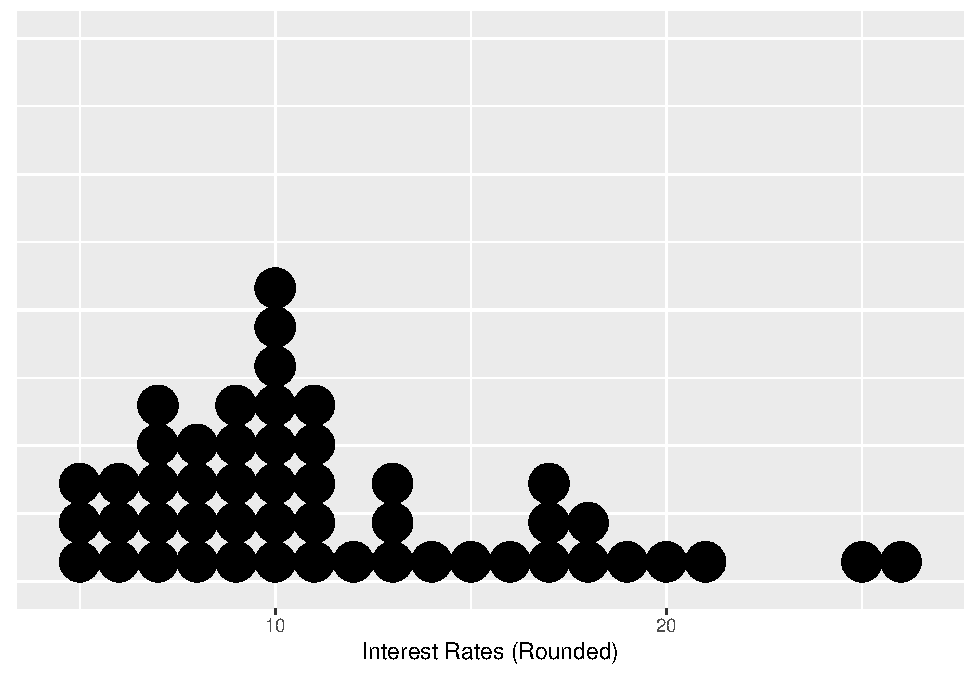
\includegraphics{bookdown-demo_files/figure-latex/dotplot-1.pdf}
\caption{\label{fig:dotplot}Dot Plot for 50 Interest Rates (rounded)}
\end{figure}

Notice there is 1 black dot that corresponds to an interest rate of 20 (presumably in percent), so there is one applicant who has a rounded interest rate of 20 percent. There are 8 black dots that correspond to an interest rate to 10 percent, so there are 8 applicants with a rounded interest rate of 10 percent. So interest rates of 10 percent are much more commonly occurring than interest rate of 20 percent. So we can use the height, or number of dots, to help us glean how often the value of a certain interest rate occurs. Based on this dotplot, interest rates between 5 and 11 percent are common, with higher values being less common.

\emph{Note:} do not get too torn up about the details in the code to produce this dot plot. I have chosen the present the dot plot this way to highlight how we use it, without getting bogged down in the details of how it can be produced. We will not be using dot plots in this class.

\subsection{Histograms}\label{histograms}

It turns out that dot plots are often not useful for large data sets, but they provide the general idea of how other visualizations for larger data sets work. The height of the dots inform us about the frequency of those values occurring.

A visualization that is more commonly used for larger data sets is a \textbf{histogram}. Instead of displaying how common each value of the variable exists, we think of the values as belonging to a \textbf{bin} of values. For example, we can create a bin that contains interest rates between 5 and 7.5 percent, another bin containing interest rates between 7.5 and 10 percent, and so on. A few things to note about histograms:

\begin{itemize}
\item
  By convention, values that lie exactly on the boundary of a bin will belong to the lower bin. For example, an interest rate that is exactly 12.5 percent will belong to the bin between 10 and 12.5 percent, and not the bin between 12.5 to 15 percent.
\item
  Each bin should have the same width. In our example, the width is 2.5.
\end{itemize}

We create this histogram (using the original interest rates) below, per Figure \ref{fig:hist}:

\begin{Shaded}
\begin{Highlighting}[]
\DocumentationTok{\#\#set up sequence to specify the bins}
\NormalTok{s25}\OtherTok{\textless{}{-}}\FunctionTok{seq}\NormalTok{(}\DecValTok{5}\NormalTok{,}\FloatTok{27.5}\NormalTok{,}\FloatTok{2.5}\NormalTok{)}

\FunctionTok{ggplot}\NormalTok{(Data,}\FunctionTok{aes}\NormalTok{(}\AttributeTok{x=}\NormalTok{interest\_rate))}\SpecialCharTok{+}
  \FunctionTok{geom\_histogram}\NormalTok{(}\AttributeTok{breaks=}\NormalTok{s25,}\AttributeTok{fill=}\StringTok{"blue"}\NormalTok{,}\AttributeTok{color=}\StringTok{"orange"}\NormalTok{)}\SpecialCharTok{+}
  \FunctionTok{labs}\NormalTok{(}\AttributeTok{x=}\StringTok{"Interest Rate"}\NormalTok{, }\AttributeTok{title=}\StringTok{"Histogram of Interest Rates"}\NormalTok{)}
\end{Highlighting}
\end{Shaded}

\begin{figure}
\centering
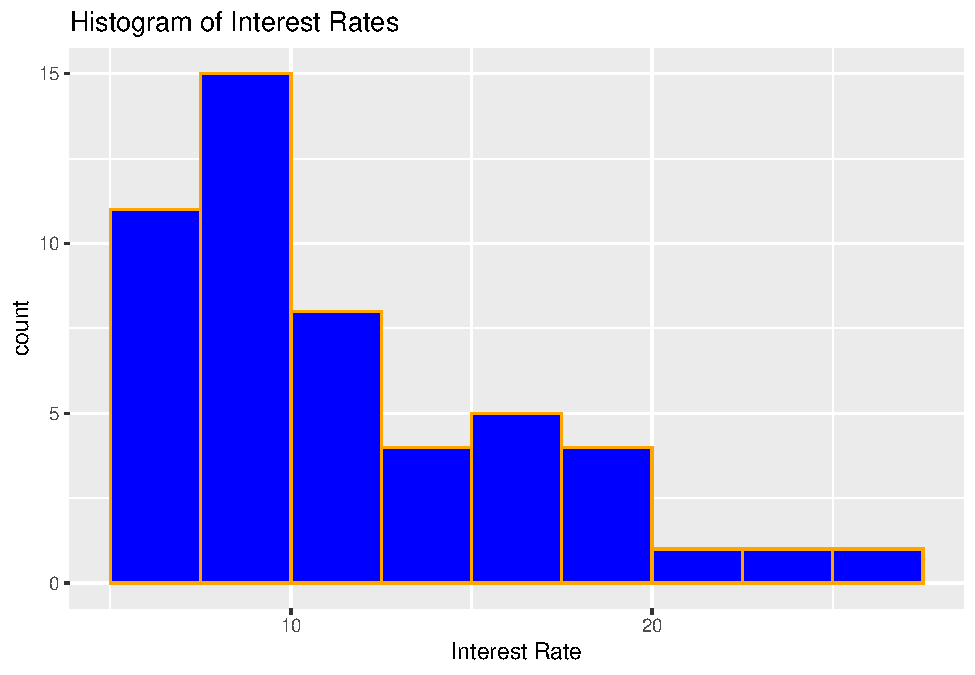
\includegraphics{bookdown-demo_files/figure-latex/hist-1.pdf}
\caption{\label{fig:hist}Historgram for 50 Interest Rates}
\end{figure}

Similar to the dot plot in Figure \ref{fig:dotplot}, the height of the histogram inform us what values are more commonly occurring. We can see from this histogram that interest rates between 5 and 10 percent are common, much more so than loans with interest rates greater than 20 percent. We could say that we have more certainty that a randomly selected loan applicant will have an interest rate between 5 and 10 percent than an interest rate that is greater than 20 percent.

\subsubsection{Shapes of Distribution}\label{shapes-of-distribution}

Histograms can also give us an idea about the \textbf{shape} of the distribution of interest rates. For the histogram in Figure \ref{fig:hist}, most of the loans are less than 15 percent, with only a small number of loans greater than 20 percent. We can say that we have greater certainty that a loan will have an interest rate less than 15 percent. When the data tail off to the right as in our histogram, the shape is said to be \textbf{right-skewed}. When a variable is said to be right-skewed, large values of the variable are much less common than small values of the variable; smaller values are more likely occur.

\begin{itemize}
\item
  If the histogram has the reverse characteristic, i.e.~the data tail off to the left instead, the shape is said to be \textbf{left-skewed}. This implies that small values of the variable are much less common than large values of the variable; larger values are more likely to occur.
\item
  Histograms that tail off similarly in both directions are called \textbf{symmetric}. Large and small values are of the variable are equally likely.
\item
  Histograms that have a peak in the middle, and then tail off on both sides are not only symmetric, but also \textbf{bell-shaped}, or have a \textbf{normal} distribution. Note: it turns out one of the assumptions in linear regression is that the response variable follow a normal distribution. This may seem restrictive, however, we will see in later modules that this assumption is not particularly crucial under some circumstances.
\end{itemize}

\emph{Thought question:} Can you think of real life variables that have symmetric, right-skewed, left-skewed distributions? Feel free to search the internet for examples.

\subsubsection{Considerations with Histograms}\label{considerations-with-histograms}

With our interest rate example, you may have noticed that I made a specific choice on the width of the bins when I created the histograms. It turns out that the width of the bins can impact the shape of the histogram, and potentially, how we interpret the histogram.

Consider creating a histogram with bin width of 0.5, instead of 2.5, per Figure \ref{fig:hist05}:

\begin{Shaded}
\begin{Highlighting}[]
\DocumentationTok{\#\#set up sequence to specify the bins. width now 0.5}
\NormalTok{s05}\OtherTok{\textless{}{-}}\FunctionTok{seq}\NormalTok{(}\DecValTok{5}\NormalTok{,}\FloatTok{27.5}\NormalTok{,}\FloatTok{0.5}\NormalTok{)}

\FunctionTok{ggplot}\NormalTok{(Data,}\FunctionTok{aes}\NormalTok{(}\AttributeTok{x=}\NormalTok{interest\_rate))}\SpecialCharTok{+}
  \FunctionTok{geom\_histogram}\NormalTok{(}\AttributeTok{breaks=}\NormalTok{s05,}\AttributeTok{fill=}\StringTok{"blue"}\NormalTok{,}\AttributeTok{color=}\StringTok{"orange"}\NormalTok{)}\SpecialCharTok{+}
  \FunctionTok{labs}\NormalTok{(}\AttributeTok{x=}\StringTok{"Interest Rate"}\NormalTok{, }\AttributeTok{title=}\StringTok{"Histogram of Interest Rates"}\NormalTok{)}
\end{Highlighting}
\end{Shaded}

\begin{figure}
\centering
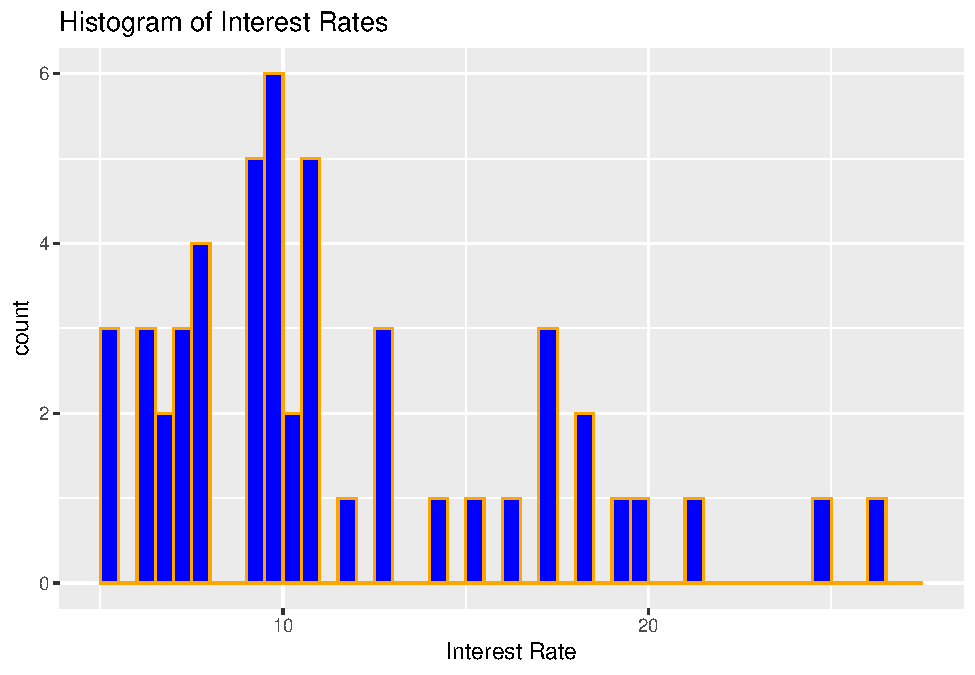
\includegraphics{bookdown-demo_files/figure-latex/hist05-1.pdf}
\caption{\label{fig:hist05}Historgram for 50 Interest Rates, with Bin Width 0.5}
\end{figure}

Comparing Figure \ref{fig:hist05} with Figure \ref{fig:hist}, note the following:

\begin{itemize}
\item
  Visually, the histogram looks more jagged with smaller bin width, whereas the histogram looks smoother with a larger bin width.
\item
  Smaller bin widths may be preferred if we need information about smaller ranges of interest rates. However, it can be difficult to write about general trends.
\item
  Larger bin widths may be more useful if we are trying to look for more general trends in the interest rates.
\end{itemize}

\emph{Thought question}: What happens if we create a histogram with a bin width that is too large?

\subsection{Density Plots}\label{densplots}

Another visualization for a quantitative variable is a \textbf{density plot}. A density plot can be viewed as a smoothed version of the histogram. We can use the heights to inform us about what values are more common. We create a density plot for the interest rates in Figure \ref{fig:dens}:

\begin{Shaded}
\begin{Highlighting}[]
\DocumentationTok{\#\#density plot}
\FunctionTok{plot}\NormalTok{(}\FunctionTok{density}\NormalTok{(Data}\SpecialCharTok{$}\NormalTok{interest\_rate), }\AttributeTok{main=}\StringTok{"Density Plot of Interest Rates"}\NormalTok{)}
\end{Highlighting}
\end{Shaded}

\begin{figure}
\centering
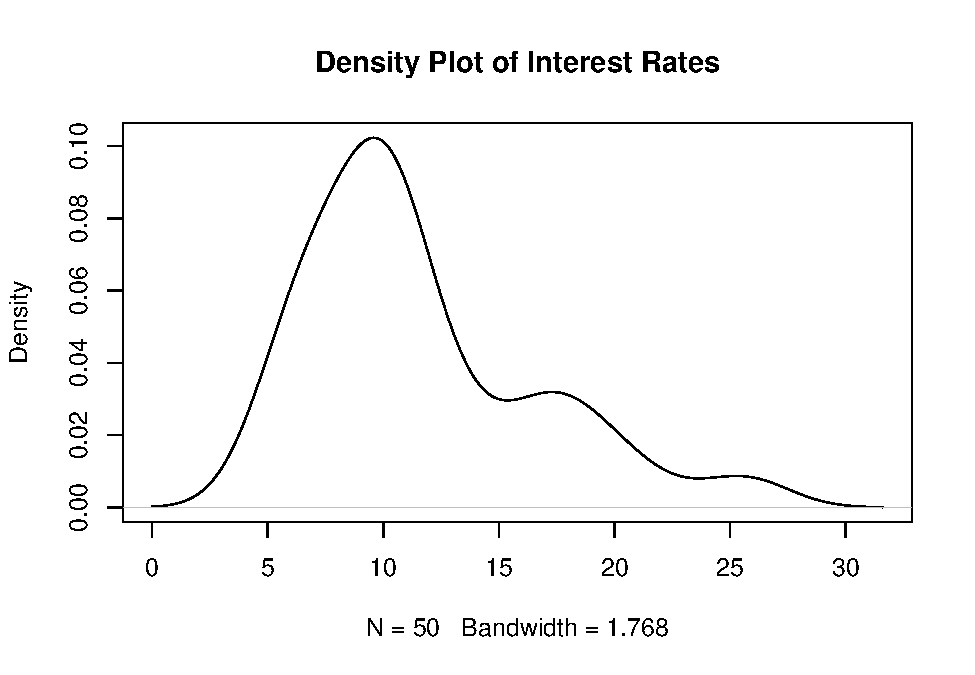
\includegraphics{bookdown-demo_files/figure-latex/dens-1.pdf}
\caption{\label{fig:dens}Density Plot for 50 Interest Rates}
\end{figure}

Based on Figure \ref{fig:dens}, we see that low interest rates (between 5 and 12.5 percent) are much more common and high interest rates (higher than 20 percent). A few things to note about interpreting density plots:

\begin{itemize}
\tightlist
\item
  The area under the density plot is always equals to 1.
\item
  To find the proportion of interest rates that are between two values, for example between 10 and 15 percent, we would integrate this density plot over this range, i.e.~\(\int_{10}^{15} f(x) dx\), where \(f(x)\) is a mathematical equation that describes the density plot. We will learn about this equation in more detail in a later module.
\item
  The values on the vertical axis do not equal to probabilities (a common misconception).
\end{itemize}

The density plot is found using a method called kernel density estimation (KDE). We will over details about KDE in Section \ref{KDE} as we need to cover quite a bit of material before doing so.

\subsubsection{Considerations with Density Plots}\label{considerations-with-density-plots}

Similar to bins and histograms, density plots are affected by the \textbf{bandwidth}. Larger bandwidths lead to smoother density plots, while smaller bandwidths lead to more jagged density plots. We create a density plot that uses a bandwidth that is twice the default in Figure \ref{fig:dens2} below:

\begin{Shaded}
\begin{Highlighting}[]
\FunctionTok{plot}\NormalTok{(}\FunctionTok{density}\NormalTok{(Data}\SpecialCharTok{$}\NormalTok{interest\_rate, }\AttributeTok{adjust=}\DecValTok{2}\NormalTok{), }\AttributeTok{main=}\StringTok{"Density Plot of Interest Rates, with Bandwidth Twice the Default"}\NormalTok{)}
\end{Highlighting}
\end{Shaded}

\begin{figure}
\centering
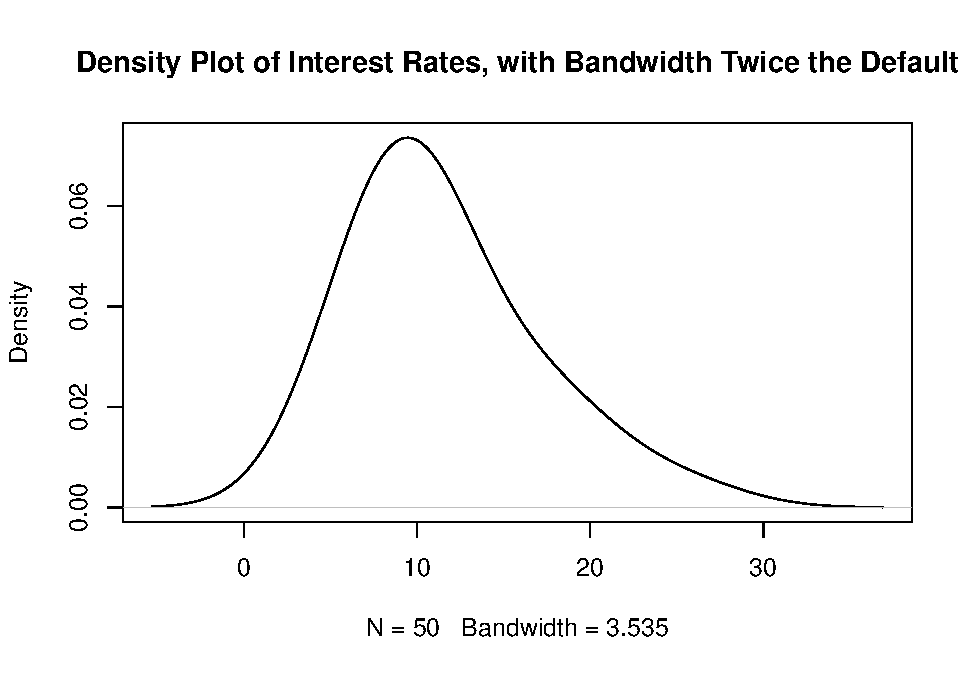
\includegraphics{bookdown-demo_files/figure-latex/dens2-1.pdf}
\caption{\label{fig:dens2}Density Plot for 50 Interest Rates with Larger Bandwidth}
\end{figure}

Notice in Figure \ref{fig:dens2} that the little peak for interest rates between 15 and 20 (which existed in Figures \ref{fig:dens} and also \ref{fig:hist}) no longer exists. Using bandwidths that are too large can smooth out some of these peaks.

\emph{Thought question}: How are bin widths for histograms and bandwidths for density plots related?

\section{Ordered Statistics}\label{ordered-statistics}

The idea behind ordered statistics is pretty self-explanatory: take your numerical variable, and order the values from smallest to largest. Going back to our example of the interest rates from 50 loan applicants, let \(X\) denote the interest rate. Then \(x_{(1)}\) will denote the interest rate that is the smallest, \(x_{(2)}\) denotes the second smallest interest rate, and \(x_{(50)}\) denotes the largest interest rate in our sample of 50.

\subsection{Quantiles}\label{quantiles}

\textbf{Quantiles} partition the range of numerical data into continuous intervals (groups) with (nearly) equal proportions. Common quantiles have their own names:

\begin{itemize}
\tightlist
\item
  Quartiles: 4 groups
\item
  Percentiles: 100 groups
\end{itemize}

We will go over quartiles in more detail.

\subsubsection{Quartiles}\label{quart}

Quartiles divide the data into 4 groups, and each group has (nearly) equal number of observations. So there will be three quartiles, denoted by \(Q_1, Q_2, Q_3\).

\begin{itemize}
\tightlist
\item
  The first group will have values between negative infinity and \(Q_1\).
\item
  The second group will have values between negative \(Q_1\) and \(Q_2\).
\item
  The third group will have values between negative \(Q_2\) and \(Q_3\).
\item
  The fourth group will have values between negative \(Q_3\) and infinity.
\end{itemize}

\(Q_2\), sometimes called the second quartile, is the easiest value to find. It is also called the \textbf{median} of the data. Going back to our interest rates from the 50 loan applicants. Using our ordered statistics, the median is the middle observation. Since we have an even number of observations, we have two middle observations, \(x_{(25)}\) and \(x_{(26)}\). In this situation, the median will be the average of these two middle observations. Using R, we find the median to be:

\begin{Shaded}
\begin{Highlighting}[]
\FunctionTok{median}\NormalTok{(Data}\SpecialCharTok{$}\NormalTok{interest\_rate)}
\end{Highlighting}
\end{Shaded}

\begin{verbatim}
## [1] 9.93
\end{verbatim}

So roughly half the interest rates are less than 9.93 percent, and roughly half the interest rates are greater than 9.93 percent. You might also recognize another term for the median: the 50th percentile, as 50 percent of the interest rates are less than 9.93.

To find the middle observation(s) based on a sample of size \(n\):

\begin{itemize}
\tightlist
\item
  If \(n\) is even, the 2 middle observations will be position \(\frac{n}{2}\) and \(\frac{n}{2} + 1\) in the ordered statistics.
\item
  If \(n\) is odd, the middle observation will be position \(\frac{n}{2} + 0.5\) in the ordered statistics.
\end{itemize}

\(Q_1\) and \(Q_3\) (also called the first and third quartiles) are found together, after finding \(Q_2\). Note that \(Q_2\) divides the data into two groups. Using our interest rates example, one group contains \(x_{(1)}, \cdots, x_{(25)}\), and another group contains \(x_{(26)}, \cdots, x_{(50)}\). \(Q_1\) is the median of the first group, and \(Q_3\) is the median of the second group. So for our 50 loan applicants:

\begin{itemize}
\tightlist
\item
  \(Q_1\) is \(x_{(13)}\), and
\item
  \(Q_3\) is \(x_{(38)}\).
\end{itemize}

To find these values in R, we could type:

\begin{Shaded}
\begin{Highlighting}[]
\FunctionTok{quantile}\NormalTok{(Data}\SpecialCharTok{$}\NormalTok{interest\_rate, }\AttributeTok{prob=}\FunctionTok{c}\NormalTok{(}\FloatTok{0.25}\NormalTok{,}\FloatTok{0.75}\NormalTok{), }\AttributeTok{type =} \DecValTok{1}\NormalTok{)}
\end{Highlighting}
\end{Shaded}

\begin{verbatim}
##   25%   75% 
##  7.96 14.08
\end{verbatim}

So \(Q_1\) is 7.96 percent, and \(Q_3\) is 14.08 percent. It turns out that \(Q_1\) is also the 25th percentile, and \(Q_3\) is also the 75th percentile, by definition.

Remember we wrote the following earlier:

\begin{itemize}
\tightlist
\item
  The first group will have values between negative infinity and \(Q_1\). So about a quarter of observations are have interest rates less than 7.96 percent.
\item
  The second group will have values between negative \(Q_1\) and \(Q_2\). So about a quarter of observations have interest rates between 7.96 and 9.93 percent.
\item
  The third group will have values between negative \(Q_2\) and \(Q_3\). So about a quarter of observations have interest rates between 9.93 and 14.08 percent.
\item
  The fourth group will have values between negative \(Q_3\) and infinity. So about a quarter of observations have interest rates above 14.08 percent.
\end{itemize}

Note: you may notice that we used \texttt{type\ =\ 1} inside the \texttt{quantile()} function. Using \texttt{type\ =\ 1} gives the values of the first and third quartiles that are based on the method that was just described. There are actually several ways to find quantiles, which may result in slightly differing values, although they all generally meet the definition that \(Q_1\) is the 25th percentile, and \(Q_3\) is the 75th percentile.

\subsubsection{Percentiles}\label{percentiles}

Another common quantile is the percentile. In general the \textbf{k-th percentile} is the value of the data point below which \(k\) percent of observations are found. So in our earlier example, we said that \(Q_3\) of the interest rates is 14.08 percent, and this is also the 75th percentile. So 75 percent of interest rates are less than 14.08 percent.

\subsection{Box Plots}\label{box-plots}

Another visualization used to summarize quantitative data is the box plot. A \textbf{box plot} summarizes the 5-number summary. The 5 numbers are the minimum, \(Q_1, Q_2, Q_3\), and the maximum. Using our interest rate data, the box plot is shown in Figure \ref{fig:boxplot}:

\begin{Shaded}
\begin{Highlighting}[]
\DocumentationTok{\#\#box plot}
\FunctionTok{ggplot}\NormalTok{(Data,}\FunctionTok{aes}\NormalTok{(}\AttributeTok{y=}\NormalTok{interest\_rate))}\SpecialCharTok{+}
  \FunctionTok{geom\_boxplot}\NormalTok{()}\SpecialCharTok{+}
  \FunctionTok{labs}\NormalTok{(}\AttributeTok{y=}\StringTok{"Interest Rate"}\NormalTok{, }\AttributeTok{title=}\StringTok{"Box Plot of Interest Rates"}\NormalTok{)}
\end{Highlighting}
\end{Shaded}

\begin{figure}
\centering
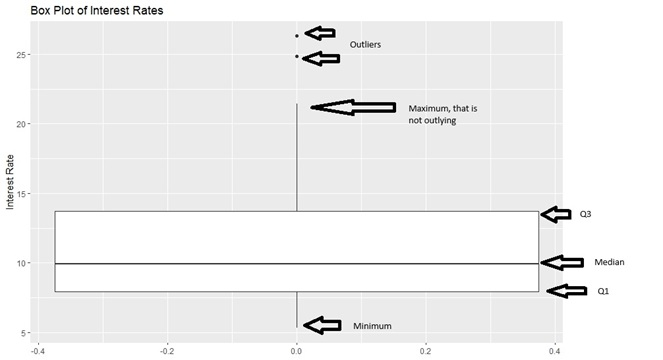
\includegraphics{images/01-boxplot.jpeg}
\caption{\label{fig:boxplot}Box Plot of Interest Rates}
\end{figure}

Some people call a box plot a box and whisker plot.

\begin{itemize}
\tightlist
\item
  The boundaries of the box represent \(Q_1\) and \(Q_3\).
\item
  The thick line in the box represents the median.
\item
  The two whiskers on either side of the box extend to the minimum and maximum, if outliers do not exist. If outliers exist, the whiskers extend to the minimum and maximum values that are not outliers.
\end{itemize}

Generally, when we have one quantitative variable, an outlier is an observation whose numerical value is far away from the rest of the data. In other words, it is a lot smaller or larger relative to the rest of the data.

So for our 50 loans, there are two loan applicants with interest rates around 25 percent that are flagged as being a lot larger than the rest of the loans, which is reasonable since most of the loans are a lot smaller than 20 percent.

We will not go over the details of how outliers are determined in box plots. If you are interested, you can read Chapter 2.1.5 from \href{https://www.openintro.org/book/os/}{OpenIntro Statistics (Diez, Ceytinka-Rundel, Barr)}. Generally, when we are working with one variable, outliers are observations which are a lot larger or smaller than the rest of the observations.

Notice how much further large values (\(Q_3\) and maximum) are from the median, compared to the distance of the small values (\(Q_1\) and minimum) from the median. This indicates that the distribution of interest rates are right-skewed. Compare the boxplot of the interest rates in Figure \ref{fig:boxplot} with its corresponding histogram (Figure \ref{fig:hist}) and density plot (Figure \ref{fig:dens}).

\emph{Thought question}: can you sketch a box plot that represents a variable that is left-skewed? How about a variable that is symmetric?

\subsection{Empirical Cumulative Distribution Function}\label{ecdf}

From the previous sections, we can see how we could use histograms, density plots, and box plots to inform us about what proportion of observations take certain values, and the values of the data that correspond to certain percentiles. However, we are limited to quartiles and not any percentile when using box plots, and we need to find areas under the density plot (using integration, not a trivial task), or add up frequencies on a histogram (can be time consuming).

A plot that can easily give us values of the variable that correspond to percentiles is the \textbf{empirical cumulative distribution function (ECDF)} plot.

Let \(X\) denote a random variable, and we have observed \(n\) observations of \(X\) denoted by \(x_1, \cdots, x_n\). Let \(x_{(1)}, \cdots x_{(n)}\) denote the ordered statistics of the \(n\) observations. The ECDF, denoted by \(\hat{F}_n(x)\) is the proportion of sample observations less than or equal to the value \(x\) of the random variable. Mathematically, the ECDF is:

\[
 \hat{F}_n(x) = 
  \begin{cases} 
   0, & \text{for } x < x_{(1)} \\
   \frac{k}{n},       & \text{for } x_{(k)} \leq x < x_{(k+1)}, k = 1, \cdots, n-1\\
   1, & \text{for } x \geq x_{(n)}.
  \end{cases}
\]
We shall use a simple toy example to illustrate how an ECDF is constructed. Suppose we ask 5 people how many times to go to the gym (at least 20 minutes) in a typical work week. The answers are: 3, 0, 1, 5, 3. The random variable \(X\) is how many times a person goes to the gym for at least 20 minutes, and the ordered statistics are \(x_{(1)} = 0, x_{(2)} = 1, x_{(3)} = 3, x_{(4)} = 3, x_{(5)} = 5\). Using the mathematical definition for the ECDF, we have:

\begin{itemize}
\tightlist
\item
  \(\hat{F}_n(x) = 0\) for \(x < x_{(1)} = 0\).
\item
  \(\hat{F}_n(x) = \frac{1}{5}\) for \(0 \leq x < x_{(2)} = 1\).
\item
  \(\hat{F}_n(x) = \frac{2}{5}\) for \(1 \leq x < x_{(3)} = 3\).
\item
  \(\hat{F}_n(x) = \frac{4}{5}\) for \(3 \leq x < x_{(5)} = 5\). This value is special for this example since we have two observations where \(x=3\).
\item
  \(\hat{F}_n(x) = 1\) for \(x \geq 5\).
\end{itemize}

The corresponding ECDF plot is shown in Figure \ref{fig:ecdf}:

\begin{Shaded}
\begin{Highlighting}[]
\DocumentationTok{\#\#toy data}
\NormalTok{y}\OtherTok{\textless{}{-}}\FunctionTok{c}\NormalTok{(}\DecValTok{3}\NormalTok{, }\DecValTok{0}\NormalTok{, }\DecValTok{1}\NormalTok{, }\DecValTok{5}\NormalTok{, }\DecValTok{3}\NormalTok{)}
\DocumentationTok{\#\#ECDF plot}
\FunctionTok{plot}\NormalTok{(}\FunctionTok{ecdf}\NormalTok{(y), }\AttributeTok{main =} \StringTok{"ECDF for Toy Example"}\NormalTok{)}
\end{Highlighting}
\end{Shaded}

\begin{figure}
\centering
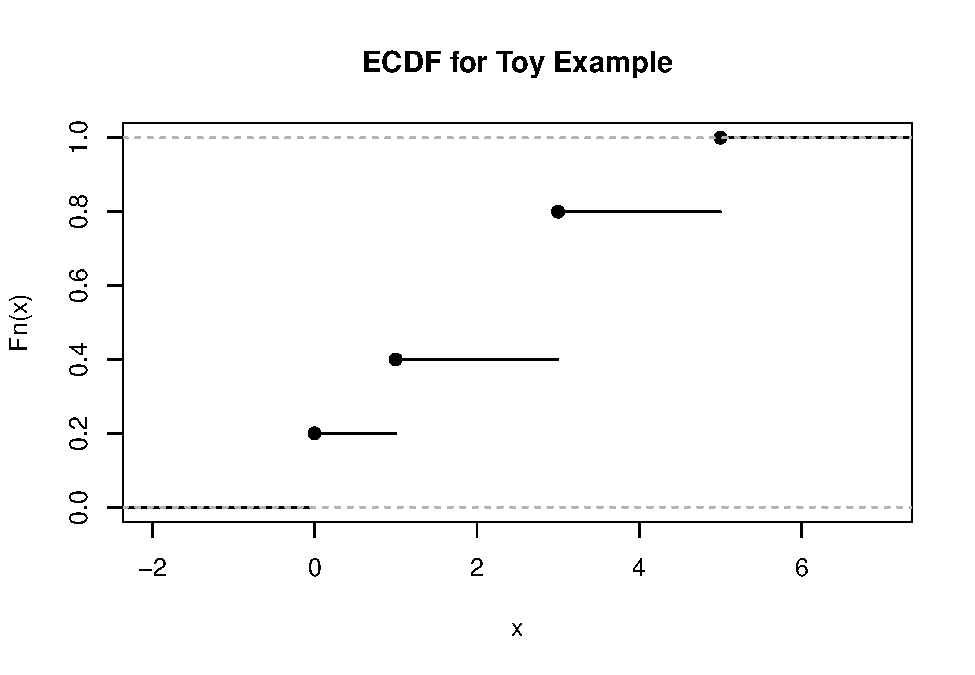
\includegraphics{bookdown-demo_files/figure-latex/ecdf-1.pdf}
\caption{\label{fig:ecdf}ECDF Plot for Toy Example}
\end{figure}

We can easily find percentiles from this plot, for example, the 40th percentile is equal to 1, going to the gym once a week. About 20 percent of observations go to the gym less than 1 time a week. The video below explains the construction of the ECDF:

Next, we create the ECDF plot for the interest rates from the 50 loan applicants.

\begin{Shaded}
\begin{Highlighting}[]
\FunctionTok{plot}\NormalTok{(}\FunctionTok{ecdf}\NormalTok{(Data}\SpecialCharTok{$}\NormalTok{interest\_rate), }\AttributeTok{main =} \StringTok{"ECDF Plot of Interest Rates"}\NormalTok{)}
\FunctionTok{abline}\NormalTok{(}\AttributeTok{h=}\FloatTok{0.8}\NormalTok{)}
\end{Highlighting}
\end{Shaded}

\begin{figure}
\centering
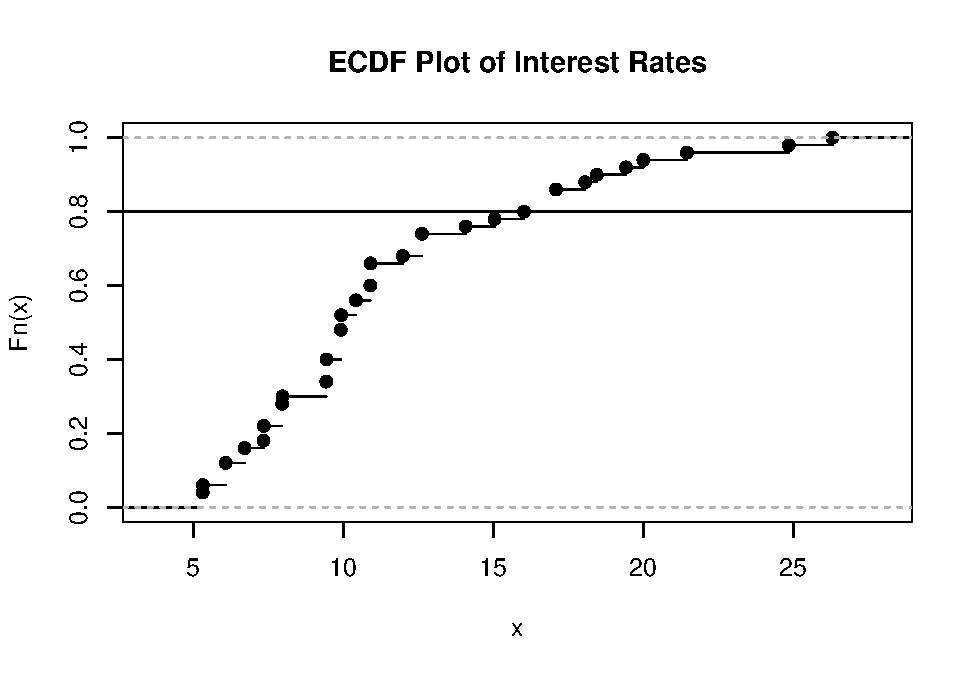
\includegraphics{bookdown-demo_files/figure-latex/ecdfreal-1.pdf}
\caption{\label{fig:ecdfreal}ECDF Plot of Interest Rates}
\end{figure}

I overlaid a horizontal line for the 80th percentile, so we can read on the horizontal axis that this corresponds to an interest rate of about 17 percent. So about 80 percent of loan applicants have an interest rate less than 17 percent.

\emph{Thought question}: try using the histogram and density plot for the interest rates (Figures \ref{fig:hist} and \ref{fig:dens}) to find the interest rate that corresponds to the 80th percentile. Was this easy to perform?

\section{Measures of Centrality}\label{measures-of-centrality}

So far, we have used visualizations to summarize the shape of the distribution of a quantitative variable. Next, we look at common measures of centrality. Loosely speaking, measures of centrality are measures that describe the average or typical value of a quantitative variable. The common measures of centrality are the mean, median, and mode.

\subsection{Mean}\label{mean}

The sample \textbf{mean} is simply the average value of the variable in our sample. The sample mean for a random variable \(X\) is denoted by \(\bar{x}\), and is found by:

\begin{equation} 
\bar{x} = \frac{\sum_{i=1}^n x_i}{n}.
\label{eq:mean}
\end{equation}

So, for our toy example of the 5 people and how often they go to the gym in a week, their sample mean is \(\bar{x} = \frac{3+0+1+5+3}{5} = 2.4\).

\subsection{Median}\label{median}

We went over how to find the median in section \ref{quart}. The \textbf{median} is the value of the middle observation in ordered statistics. It is also called \(Q_2\), the second quartile, and the 50th percentile, so approximately 50 percent of observations have values smaller than the median.

So, for our toy example of the 5 people and how often they go to the gym in a week, their sample median is \(x_{(3)} = 3\). So about 50 percent of people went to gym less than 3 times in a week.

\subsection{Mode}\label{mode}

Another measure is the mode. Mathematically speaking, the \textbf{mode} is the most commonly occurring value in the data. So for our toy example, the mode is 3, since 3 occurs twice and occurs the most often in our data.

\subsection{Considerations}\label{considerations}

A few things to consider when using these measures of centrality:

\begin{itemize}
\item
  The mean is a measure that most people are comfortable with, however, caution needs to be used if the variable is skewed, as extreme outliers and drastically alter the value of the mean. Using our toy example with the gym, suppose the person who visits the gym the most visits 50 times, instead of 5. The numerical value of the sample mean explodes, and does not give a good representation of the central value of how many visits to the gym a person makes in a week. The mean is fine if the variable is symmetric.
\item
  The median is a measure that is recommended for skewed distributions, since the order associated with ordered statistics is not influenced by extreme outliers. Using the gym example, in the previous bullet point, the median is unaffected.
\item
  The mean being larger than the median is an indication that the distribution is right-skewed. Using our interest rate example, we have:
\end{itemize}

\begin{Shaded}
\begin{Highlighting}[]
\FunctionTok{mean}\NormalTok{(Data}\SpecialCharTok{$}\NormalTok{interest\_rate)}
\end{Highlighting}
\end{Shaded}

\begin{verbatim}
## [1] 11.5672
\end{verbatim}

\begin{Shaded}
\begin{Highlighting}[]
\FunctionTok{median}\NormalTok{(Data}\SpecialCharTok{$}\NormalTok{interest\_rate)}
\end{Highlighting}
\end{Shaded}

\begin{verbatim}
## [1] 9.93
\end{verbatim}

which is consistent with the right skew we saw in the histogram and density plot in Figures \ref{fig:hist} and \ref{fig:dens}. Conversely, a left-skewed distribution usually has a mean that is smaller than the median. A symmetric distribution typically has similar values for the mean and median.

\begin{itemize}
\item
  The mean is considered a \textbf{sensitive} measure, since its numerical value can be drastically affected by outliers. The median is considered a \textbf{robust} measure, since its numerical value is more resistant and is less affected by outliers.
\item
  The mathematical definition of mode can be difficult to use for variables that are continuous, since it is likely that there are no observations that have the same value when the variable is continuous. In this instance, the mode typically refers to the bin in the histogram that has is the tallest. So, using the histogram in Figure \ref{fig:hist} for the interest rates, the mode is between 7.5 to 10 percent.
\end{itemize}

\section{Measures of Spread}\label{measures-of-spread}

In the previous sections, we learned about summarizing features a quantitative variable, by using visualizations to summarize its shape, and by using some measures of centrality that describe the average or typical values of the variable. One more feature we can summarize is the spread, associated with the values of a quantitative variable. Measures of spread are considered a way to measure uncertainty. Data that have larger spread have more uncertainty.

\subsection{Variance and Standard Deviation}\label{variance-and-standard-deviation}

One measure of spread is the variance. The sample \textbf{variance} for a random variable \(X\) is denoted by \(s^2\), or sometimes \(s_x^2\), and is found by:

\begin{equation} 
s^2 = \frac{\sum_{i=1}^n (x_i-\bar{x})^2}{n-1}.
\label{eq:variance}
\end{equation}

The variance can be interpreted as the approximate average squared distance of the observations from the mean. The formula in equation \eqref{eq:variance} may look a bit complicated, but let us use the toy example where we asked 5 people how often they go to the gym in a workweek. The answers are: 3, 0, 1, 5, 3, and we had earlier found the sample mean to be \(\bar{x} = 2.4\). To calculate the sample variance:

\[
\begin{split}
s^2 &= \frac{\sum_{i=1}^n (x_i-\bar{x})^2}{n-1}\\
 &= \frac{(3-2.4)^2 + (0-2.4)^2 + (1-2.4)^2 + (5-2.4)^2 + (3-2.4)^2}{5-1} \\
&= 3.8 
\end{split}
\]

Notice what we did in the numerator of equation \eqref{eq:variance}: we take the difference between each observed value from the sample mean, square these differences, then add up the squared differences. We then divide by \(n-1\), rather than \(n\), hence the sample variance being the approximate averaged squared distance of the observations from the mean. There is some nuance in the mathematics as to why we divide by \(n-1\) instead of \(n\), and may not be intuitive as to why we do so. It turns out dividing by \(n-1\) makes the sample variance an unbiased estimator of the true variance in the population (denoted by \(\sigma^2\)) and is more reliable than if we had divided by \(n\). We will go over this in more detail in a later module after covering a few additional concepts.

The video below explains the calculation of the sample variance:

Larger values of the sample variance indicate that the observations are generally further away from the sample mean, indicating larger spread, and a higher degree of uncertainty about future values.

\emph{Thought question}: What does it mean if the sample variance of a set of observations is 0? Why does this indicate their there is little (or no) uncertainty about the set of observations?

Another related measure is the sample \textbf{standard deviation}, which is the square root of the sample variance. Similar to the variance, larger values indicated more spread in the data.

\subsection{Interquartile Range}\label{interquartile-range}

Another measure of spread is the \textbf{interquartile range (IQR)}, and it is the difference between the third and first quartiles,

\begin{equation} 
IQR = Q_3 - Q_1.
\label{eq:IQR}
\end{equation}

The IQR is considered a robust measure of spread, while the sample variance and standard deviations are considered to be sensitive.

\chapter{Probability}\label{probability}

This module is based on Introduction to Probability (Blitzstein, Hwang), Chapters 1 and 2. You can access the book for free at \url{https://stat110.hsites.harvard.edu/} (and then click on Book). Please note that I cover additional topics, and skip certain topics from the book. You may skip: Sections 1.4, 1.5, Theorem 1.6.3, Examples 1.6.4, 2.4.5, 2.5.12, 2.7.3 from the book.

\section{Introduction to Probability}\label{introduction-to-probability}

A way of quantifying uncertainty is through probability. Think about these statements: ``I am 100\% certain that it will rain in the next hour'' and ``I am 50\% certain that it will rain in the next hour''. The percentages are used to reflect the degree of certainty about the event happening. The first statement reflects certainty; the second reflects uncertainty as the statement implies the belief that it is equally likely that it will rain or not. In this module, we will learn about the basic concepts about probability.

\subsection{Why Study Probability?}\label{why-study-probability}

The book (Section 1.1) lists 10 different applications of probability, and there are many more applications. I will go as far as to say that anything that deals with data will also deal with probability.

\subsection{Frequentiest and Bayesian View of Probability}\label{frequentiest-and-bayesian-view-of-probability}

There are a couple of viewpoints on how to interpret probability: \textbf{frequentist} and \textbf{Bayesian}. Consider the statement that ``if we flip a fair coin, the coin has a 50\% chance of landing heads''.

\begin{itemize}
\item
  The frequentist viewpoint views probability as the relative frequency associated with an event that is repeated for an infinite number of times. It will interpret the 50\% probability as: if we were to flip the coin many many times, 50\% of these times will result in the coin landing heads.
\item
  The Bayesian viewpoint views probability as a measure of belief, or certainty, that an event will happen. It will interpret the 50\% probability as: heads and tails are equally likely to occur with a coin flip.
\end{itemize}

In this coin flip example, both interpretations are reasonable. However, in some instances, the frequentist interpretation may not be as interpretable if we cannot repeat the event many times. For example, the earlier statement about rain: ``I am 50\% certain that it will rain in the next hour''. Whether it will rain or not in the next hour is not a repeatable event, so the frequentist interpretation makes less sense here.

\section{Key Concepts in Probability}\label{key-concepts-in-probability}

In this section, we will cover the basic terminology and foundational ideas in probability.

\subsection{Sample Space}\label{sample-space}

The \textbf{sample space} of an experiment, denoted by \(S\), is the set of all possible outcomes of an experiment.

For the rest of this module, we will use the following as an example: consider a standard deck of 52 cards, and we draw one card at random. What is the card drawn? The sample space for this experiment can be viewed as a list of all 52 cards, per Figure \ref{fig:cards} below.

\begin{figure}
\centering
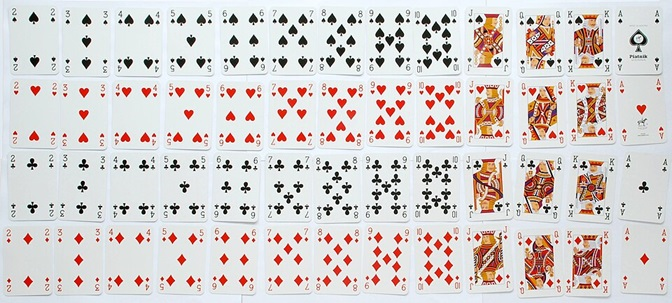
\includegraphics{images/02-cards.jpg}
\caption{\label{fig:cards}Sample Space of Drawing One Card from Standard Deck. Picture from \url{https://en.wikipedia.org/wiki/Standard_52-card_deck}}
\end{figure}

While the definition of sample space may appear elementary, writing out the sample space is almost always the first step in performing any probability calculations.

\subsection{Event}\label{event}

An \textbf{event} is a subset of the sample space, and is usually denoted by an upper case letter. For example, let \(A\) denote the event that I draw a card with a black suit (spades or clubs), and let \(B\) denote the event I draw a picture card (Jack, Queen, or King). Events \(A\) and \(B\) are each shown in Figures Figure \ref{fig:cardsA} and Figure \ref{fig:cardsB} below.

\begin{figure}
\centering
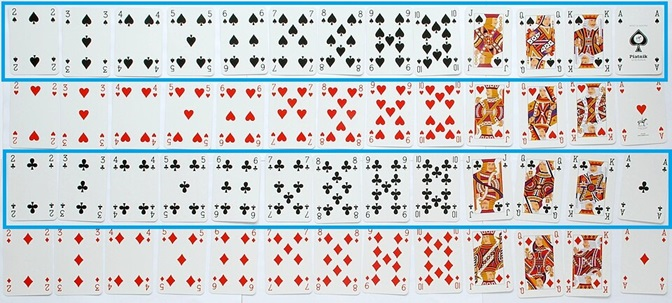
\includegraphics{images/02-cardsA.jpg}
\caption{\label{fig:cardsA}Event \(A\) (in Blue)}
\end{figure}

\begin{figure}
\centering
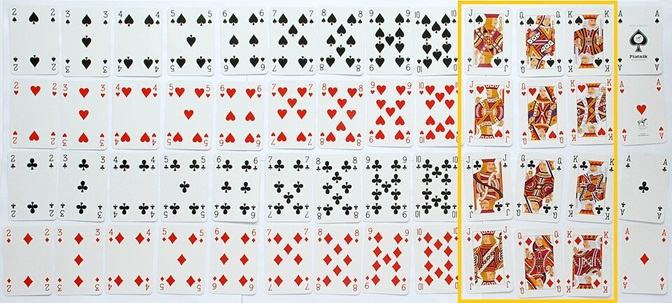
\includegraphics{images/02-cardsB.jpg}
\caption{\label{fig:cardsB}Event \(B\) (in gold)}
\end{figure}

The sample space of the experiment can be finite or infinite. In our card example, our sample space is finite since we can actually write out all possible outcomes. If the number of possible outcomes is infinite (i.e.~we cannot write out the entire list of all possible outcomes), the sample space is infinite.

We assign a probability to each event. The probability of event \(A\) happening is \(P(A)\). \textbf{If each outcome of a sample space is equally likely and we have a finite sample space, the probability of the event is the number of outcomes belonging to the event divided by the number of outcomes in the sample space.} Using our card example, \(P(A) = \frac{26}{52} = \frac{1}{2}\) and \(P(B) = \frac{12}{52} = \frac{3}{13}\).

\subsection{Complements}\label{complements}

The \textbf{complement} of an event is the set of all outcomes that do not belong to the event. For example, the complement of \(A\), denoted by \(A^c\), will be drawing a card with a red suit (hearts or diamonds). One way to think about complements is that the complement of an event is the event not happening. Looking at Figure \ref{fig:cardsA}, this will be the cards that are not outlined in blue. In this example, \(P(A^c) = \frac{26}{52} = \frac{1}{2}\).

\emph{Thought question}: What is the probability of drawing a non picture card?

From these examples, you might realize the probability associated with the complement of an event can be found by subtracting the probability of the event from 1, i.e.

\begin{equation} 
P(A^c) = 1 - P(A).
\label{eq:comp}
\end{equation}

Sometimes, the calculation for the probability of the complement of an event is much less tedious than the probability of the event. In such an instance, equation \eqref{eq:comp} will be useful.

\subsection{Unions}\label{unions}

The \textbf{union} of events is when \textbf{at least one} of the events happen. For example, the union of events \(A\) and \(B\), denoted by \(A \cup B\), is the event that the card drawn is either a black suit, or a picture card, or both a black suit and a picture card. This is reflected in Figure \ref{fig:cardsAB}.

\begin{figure}
\centering
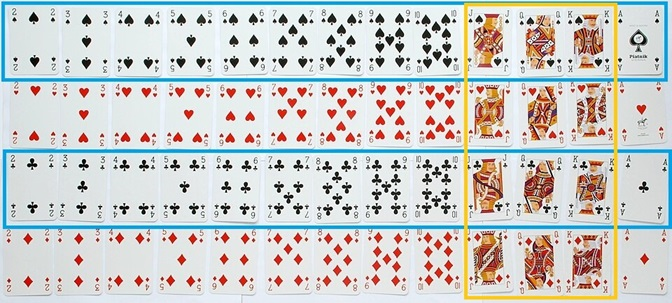
\includegraphics{images/02-cardsAB.jpg}
\caption{\label{fig:cardsAB}Union of A, B (in blue or gold, or both blue and gold)}
\end{figure}

To find \(P(A \cup B)\), we can refer to Figure \ref{fig:cardsAB} and just count the number of outcomes to belong to either event \(A\) (is black suit) or event \(B\) (is picture card), and find this is \(\frac{32}{52}\).

The union of \(A\) and \(B\) can be viewed as the event where either event \(A\) or \(B\) (or both) happens.

\subsection{Intersections}\label{intersections}

The \textbf{intersection} of events is when \textbf{all} of the events happen. Using our example, the intersection of events \(A\) and \(B\) is denoted by \(A \cap B\), is the event that the card drawn is both a black suit and a picture card. Using Figure \ref{fig:cardsAB}, the outcomes belonging to \(A \cap B\) are the cards that are outlined in blue and gold. This probability is \(P(A \cap B) = \frac{6}{52}\).

\subsection{Addition Rule}\label{addition-rule}

A common mistake that can be made in calculating \(P(A \cup B)\) is to just add up the probabilities of each individual event, so the mistake will say this probability is \(\frac{26}{52} + \frac{12}{52} = \frac{38}{52}\). The problem with this approach is that the outcomes that belong to both events (black picture cards) get counted twice, when we only want to count them once. This leads to the following formula for calculating probabilities involving unions of two events, and is sometimes called the \textbf{addition rule} in probability:

\begin{equation} 
P(A \cup B) = P(A) + P(B) - P(A \cap B).
\label{eq:union}
\end{equation}

Using equation \eqref{eq:union}, \(P(A \cup B) = \frac{26}{52} + \frac{12}{52} - \frac{6}{32} = \frac{32}{52}\).

The video below explains the addition rule with this example in a bit more detail:

\subsection{Disjoint or Mutually Exclusive Events}\label{disjoint-or-mutually-exclusive-events}

The previous discussion leads to the idea of \textbf{disjoint}, or \textbf{mutually exclusive} events. Events are disjoint if they cannot happen simultaneously. In our card example, events \(A\) and \(B\) are not disjoint, since \(A\) and \(B\) can happen simultaneously, since a card that is drawn can be both black and a picture card, e.g.~we draw a king of spades.

Using Figure \ref{fig:cardsAB} as a visual example, we can see that events \(A\) and \(B\) are not disjoint since the outcomes in blue overlap with the outcomes in gold.

Suppose we define another event, \(C\), to denote that the card drawn is an Ace. The events \(B\) and \(C\) are disjoint since a card that is drawn cannot be both a picture card and an ace. This definition of disjoint events leads to the following: for events are disjoint, the probability of their intersection will be 0.

Using Figure \ref{fig:cardsBC} below as a visual example, we can see that events \(B\) and \(C\) are disjoint since the outcomes in gold and pink do not overlap.

\begin{figure}
\centering
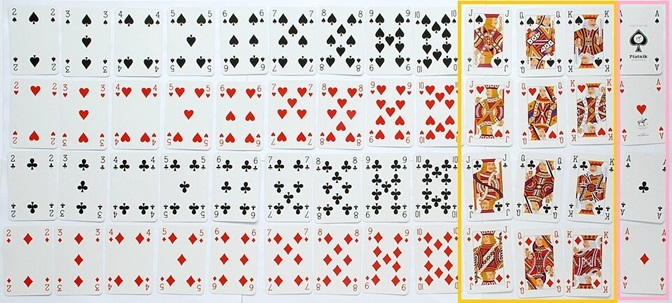
\includegraphics{images/02-cardsBC.jpg}
\caption{\label{fig:cardsBC}Events B, C (in gold and pink respectively)}
\end{figure}

Applying this idea to equation \eqref{eq:union}, we have the following for disjoint events: \textbf{for disjoint events, the probability of at least one event happening is the sum of the probabilities for each event}.

\subsection{Axioms of Probability}\label{axioms-of-probability}

The following are called the axioms of probability, which are considered foundation properties associated with probability:

\begin{enumerate}
\def\labelenumi{\arabic{enumi}.}
\tightlist
\item
  The probability of any event, \(E\), is non negative, i.e.~\(P(E) \geq 0\).
\item
  The probability that at least one outcome in the sample space occurs is 1, i.e.\(P(S) = 1\).
\item
  If \(A_1, A_2, \cdots\) are all disjoint events, then
\end{enumerate}

\[
P(\bigcup\limits_{i=1}^{\infty} A_{i}) = \sum_{i=1}^{\infty} P(A_i).
\]
In other words, for disjoint events, the probability that at least one event happens is the sum of their individual probabilities.

Note: most writers list these as three axioms. Our book combines the first two axioms into 1, and so write these as two axioms.

We can easily see how equations \eqref{eq:comp} and \eqref{eq:union} can be derived from these axioms. Note that these equations and the axioms apply in all circumstances, regardless of whether the sample space is finite or not.

\section{Conditional Probability}\label{condprob}

The concept of conditional probability appears in almost all statistical and data science models. In statistical models such as logistic regression, we are trying to use observable data (called predictors, input variables, etc) to model the probabilities associated with the different values of an outcome that is random (called response variable, output variable, etc). If the observable data are predictive of the outcome, then the probabilities associated with the outcome should indicate greater certainty, than if we do not have the observable data. Conditional probabilities allows us to incorporate observable data, or evidence, when evaluating uncertainty with random outcomes.

Consider that we are headed out for lunch, and we need to decide if we want to bring an umbrella (assuming we only bring an umbrella if we think it is going to rain). If we had been working in a windowless basement with no internet, we will have a high degree of uncertainty when evaluating if it will rain or not. However, if we were to look outside and observe the current weather conditions before heading out, we are likely to have a higher degree of certainty when evaluating if it will rain or not. Conditional probabilities allow us to incorporate what we see into our prediction of a random event.

If we were to use the language of probability to denote this example, let \(R\) denote the event that it will rain when we go for lunch. If we had been working in the windowless basement with no internet, we will be calculating \(P(R)\), the probability it will rain when we go to lunch. If we are able to incorporate the current weather conditions, this probability will be denoted as \(P(R|data)\), where data denotes the current observe weather conditions. \(P(R|data)\) can be read as the probability that it will rain when we go to lunch, given what we have observed with the weather. With this example, we can see that \(P(R)\) and \(P(R|data)\) will be different, since we update our probability given useful information. Notice the \(|\) symbol inside the probability. This symbol implies that we are working with a conditional probability, with the given or observed information listed after the \(|\).

\subsection{Definition}\label{def}

If \(X\) and \(Y\) are events, with \(P(X)>0\), the conditional probability of \(Y\) given \(X\), denoted by \(P(Y|X)\), is

\begin{equation} 
P(Y|X) = \frac{P(Y \cap X)}{P(X)}.
\label{eq:cond}
\end{equation}

In this definition, we want to update the probability of \(Y\) happening, given that we have observed \(X\). \(X\) can be viewed as the observable data or the evidence we want to incorporate.

In the Bayesian viewpoint of probability, \(P(Y)\) is called the \textbf{prior} probability of \(Y\) since it reflects our belief about \(Y\) before observing any data. \(P(Y|X)\) is called the \textbf{posterior} probability of \(Y\), as it reflects an update on our belief about \(Y\) after incorporating observed data.

Let us go back to the standard deck of cards example. Let us find \(P(B|A)\), the probability that our card is a picture card, given that we know the card is a black suit. Visually, we can use the definition of conditional probability using Figure \ref{fig:cardscond} below.

\begin{figure}
\centering
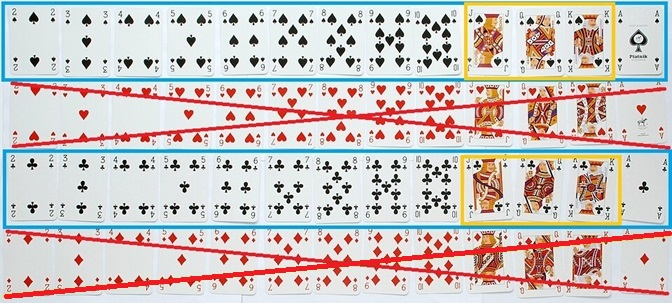
\includegraphics{images/02-cardscond.jpg}
\caption{\label{fig:cardscond}Events A, given B}
\end{figure}

We are told that our card is a black suit, so we have only 26 possible outcomes to consider, as the red cards are eliminated and are crossed out in Figure \ref{fig:cardscond}. Out of these 26 outcomes, how many are picture cards? So this probability \(P(B|A)\) is \(\frac{6}{26}\). Figure \ref{fig:cardscond} represents the frequentist viewpoint of conditional probability: \(P(B|A)\) represents the long run proportion of picture cards among cards that are black suits.

We can also apply equation \eqref{eq:cond}: \(P(B|A) = \frac{\frac{6}{52}}{\frac{1}{2}} = \frac{6}{26}\) which gives the same answer.

The video explains conditional probability with this example in a bit more detail:

\emph{Thought question}: work out the probability that the card drawn is a black suit, given that we know the card is a picture card.

We can see from this example that in general \(P(Y|X) \neq P(X|Y)\). This informs us that we need to be extremely careful when writing out our conditional probabilities and interpreting them, and knowing which one matters to our analysis. For example, the probability that I feel unwell given that I have the flu is close to 1, but the probability that I have the flu given that I feel unwell is not close to 1 (since there are many things that can make me feel unwell). This confusion regarding conditional probabilities is sometimes called the confusion of the inverse or the prosecutor's fallacy. This fallacy wrongly assumes that if the probability of a fingerprint match given that the person is innocent is small, it means that the probability that the person is innocent given a fingerprint match must also be small. Before going over this fallacy in more detail, we need to cover a few more concepts.

\subsection{Multiplication Rule}\label{multiplication-rule}

From equation \eqref{eq:cond}, we have the \textbf{multiplication rule} in probability:

\begin{equation} 
P(Y \cap X) = P(Y|X) \times P(X) = P(X|Y) \times P(Y).
\label{eq:mult}
\end{equation}

The multiplication rule is useful in finding the probability of multiple events happening, especially if the events happen sequentially. As an example, consider drawing two cards, without replacement, from a standard deck of cards. Without replacement means that after drawing the first card, it is not returned to the deck, so there will be 51 cards remaining after the first draw. Let \(D_1\) and \(D_2\) denote the events that the first draw is a diamond suit and the second draw is a diamond suit respectively. We want to find the probability that both cards drawn are diamond suits. This probability can be written as \(P(D_1 \cap D_2) = P(D_1) \times P(D_2|D_1)  = \frac{13}{52} \times \frac{12}{51}  = \frac{156}{2652}\).

\subsection{Independent Events}\label{independent-events}

Events are independent if knowledge about whether one event happens or not does not change the probability of the other event happening. This implies that if \(X\) and \(Y\) are independent events, then the definition of conditional probability simplifies to \(P(Y|X) = P(Y)\). Likewise \(P(X|Y) = P(X)\). Applying this to the multiplication rule, we have the following for multiplication rule for independent events

\begin{equation} 
P(Y \cap X) = P(Y) \times P(X).
\label{eq:mult2}
\end{equation}

The probability of all events happening is just the product of the probabilities for each individual event, if the events are all independent.

Going back to our example with the standard deck of cards, where \(A\) denotes the event that I draw a card with a black suit (spades or clubs), and \(B\) denotes the event I draw a picture card (Jack, Queen, or King). We had earlier found that \(P(B) = \frac{12}{52}\) and that \(P(B|A) = \frac{6}{26}\). Notice that these two probabilities are numerically equal, which informs us that the events are independent. Knowing whether the card is a black suit or not does not change the probability that the card is a picture card. This makes sense intuitively since the proportion of cars that are picture is the same for black and red suits.

\subsection{Bayes' Rule}\label{bayes-rule}

The definition of conditional probability in equation \eqref{eq:cond} and the multiplication rule in equation \eqref{eq:mult} give us \textbf{Bayes' rule}

\begin{equation} 
P(Y|X) = \frac{P(X|Y)P(Y)}{P(X)}.
\label{eq:bayes}
\end{equation}

Bayes' rule is useful if we want to find \(P(Y|X)\) but we only have information regarding \(P(X|Y)\) available. A fairly popular model is called linear discriminant analysis, and it models the conditional probability using Bayes' rule.

\subsection{Odds}\label{odds}

The \textbf{odds} of an event \(Y\) are

\begin{equation} 
odds(Y) = \frac{P(Y)}{P(Y^c)}.
\label{eq:odds}
\end{equation}

You may realize that the left hand side of equation \eqref{eq:odds} is equal to the left hand side of a logistic regression equation that we saw in Section \ref{eg2}.

Using equation \eqref{eq:odds}, we can switch from odds to probability easily

\begin{equation} 
P(Y) = \frac{odds(Y)}{1 + odds(Y)}.
\label{eq:odds2}
\end{equation}

\subsection{Odds Form of Bayes' Rule}\label{odds-form-of-bayes-rule}

Using Bayes' rule in equation \eqref{eq:bayes} and the definition of odds in equation \eqref{eq:odds}, we have the \textbf{odds form for Bayes' rule}

\begin{equation} 
\frac{P(Y|X)}{P(Y^c|X)} = \frac{P(X|Y)}{P(X|Y^c)} \frac{P(Y)}{P(Y^c)}. 
\label{eq:oddsbayes}
\end{equation}

\subsection{Law of Total Probability}\label{law-of-total-probability}

Let \(Y_1, Y_2, \cdots, Y_n\) be a partition of the sample space (\(Y_1, Y_2, \cdots, Y_n\) are disjoint and their union is the sample space, with \(P(Y_i) > 0\)) for all \(i\). Then

\begin{equation} 
\begin{split}
P(X) &= \sum_{i=1}^n P(X|Y_i) \times P(Y_i)\\
    &= P(X|Y_1) \times P(Y_1) + P(X|Y_2) \times P(Y_2) + \cdots + P(X|Y_n) \times P(Y_n).
\end{split}
\label{eq:total}
\end{equation}

The law of total probability informs us of a way to find the probability of \(X\). We can divide the sample space in disjoint sets \(Y_i\), find the conditional probability of \(X\) within each set, and then take a weighted sum of these conditional probabilities, weighted by \(P(Y_i)\). This is useful if the conditional probability for each set is easy to obtain.

The law of total probability in equation \eqref{eq:total} can be applied to the denominator of Bayes' rule in equation \eqref{eq:bayes} to have the following variation of Bayes' rule:

\begin{equation} 
P(Y|X) = \frac{P(X|Y)P(Y)}{\sum_{i=1}^n P(X|Y_i) \times P(Y_i)}.
\label{eq:bayes2}
\end{equation}

\subsection{Worked Example}\label{worked-example}

We consider this worked example on how to apply Bayes' rule and the law of total probability. Suppose my email can be divided into three categories: \(E_1\) denotes spam email, \(E_2\) denotes important email, and \(E_3\) denotes not important email. An email must belong to only one of these categories. Let \(F\) denote the event that the email contains the word ``free''. From past data, I have the following information:

\begin{itemize}
\tightlist
\item
  \(P(E_1) = 0.2, P(E_2) = 0.5, P(E_3) = 0.3\).
\item
  The word ``free'' appears in 99\% of spam email, so \(P(F|E_1) = 0.99\).
\item
  The word ``free'' appears in 10\% of important email, so \(P(F|E_2) = 0.1\).
\item
  The word ``free'' appears in 5\% of not important email, so \(P(F|E_3) = 0.05\).
\end{itemize}

I receive an email that has the word free. What is the probability that it is spam? So we want to find \(P(E_1|F)\).

\subsubsection{Approach 1: Using Bayes' Rule}\label{approach-1-using-bayes-rule}

Using equation \eqref{eq:bayes2}, we have

\[
\begin{split}
P(E_1|F) &= \frac{P(E_1 \cap F)}{P(F)}\\
 &= \frac{P(F|E_1) \times P(E_1)}{P(F|E_1) \times P(E_1) + P(F|E_2) \times P(E_2) + P(F|E_3) \times P(E_3)} \\
&= \frac{0.99 \times 0.2}{0.99 \times 0.2 + 0.1 \times 0.5 + 0.05 \times 0.3}\\
&= 0.7528517
\end{split}
\]

The video below goes over this approach in a little bit more detail:

\subsubsection{Approach 2: Using Tree Diagrams}\label{approach-2-using-tree-diagrams}

A tree diagram is useful in finding conditional probabilities and probabilities involving intersections. It is a visual way of displaying the information you have at hand, when you have conditional probabilities over disjoint sets and probabilities for each disjoint set. In our toy example, the disjoint sets are the type of email I receive, \(E_1, E_2, E_3\), and the conditional probabilities we have are over these disjoint sets, i.e.~\(P(F|E_1), P(F|E_2)\) and \(P(F|E_3)\). We can put this information visual by first splitting our sample space into the disjoint sets \(E_1, E_2, E_3\), and then splitting each disjoint set on whether the email has the word ``free'' (\(F\)) or not (\(F^c\)). This information is displayed in a tree diagram as in Figure \ref{fig:tree}.

\begin{figure}
\centering
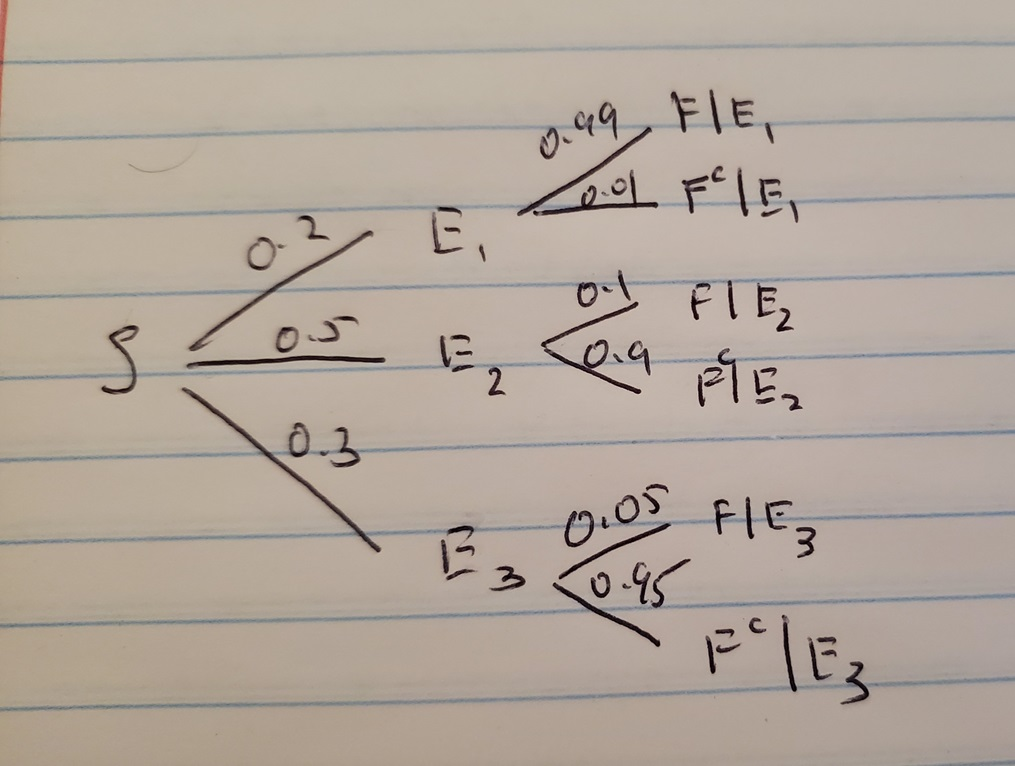
\includegraphics{images/02-tree.jpg}
\caption{\label{fig:tree}Tree Diagram for Email Example}
\end{figure}

Each split is represented by a branch, and we write the corresponding probability on each branch. We want to find the probability that a received email is spam given that it contains the word ``free'', \(P(E_1|F)\), and using the definition of conditional probability in equation \eqref{eq:cond}

\[
P(E_1|F) = \frac{P(E_1 \cap F)}{P(F)}.
\]

Looking at the tree diagram in Figure \ref{fig:tree}, we can label the branches that lead to the numerator \(P(E_1 \cap F)\), the probability that the email is spam and contains the word free. This is shown on the tree diagram below in Figure \ref{fig:tree1} below by highlighting the corresponding branches in blue.

\begin{figure}
\centering
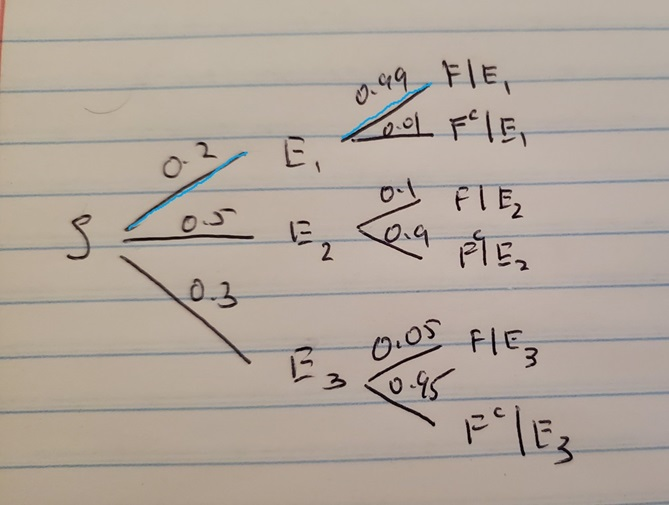
\includegraphics{images/02-treepath1.jpg}
\caption{\label{fig:tree1}Tree Diagram for Email Example, Branch for Numerator in Blue}
\end{figure}

So \(P(E_1 \cap F) = 0.2 \times 0.99 = 0.198\). We then need to find the denominator \(P(F)\). Looking at Figure \ref{fig:tree}, we can see three branches that lead to an email containing the word free: \(P(E_1 \cap F)\) or \(P(E_2 \cap F)\) or \(P(E_3 \cap F)\). This is shown on the tree diagram below in Figure \ref{fig:tree2} below by highlighting the corresponding branches in gold.

\begin{figure}
\centering
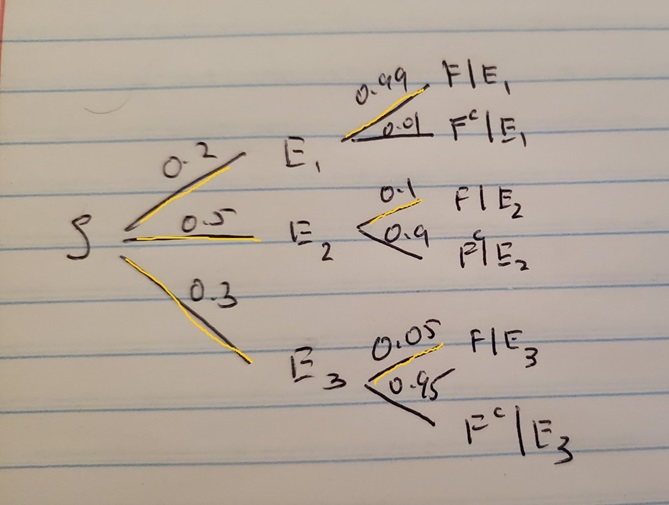
\includegraphics{images/02-treepath2.jpg}
\caption{\label{fig:tree2}Tree Diagram for Email Example, Branches for Denominator in Gold}
\end{figure}

We know the probability for each branch, and we add them up to obtain the denominator \(P(F) = 0.2 \times 0.99 + 0.5 \times 0.1 + 0.3 \times 0.05 = 0.263.\) Putting the pieces together, we have

\[
P(E_1|F) = \frac{P(E_1 \cap F)}{P(F)} = \frac{0.198}{0.263} = 0.7528517.
\]

Note: If you compare the intermediate calculations in approach 2, you end up using the calculations in approach 1, without referring to any of the associated equations.

The video below goes over tree diagrams in a little bit more detail:

\section{Confusion of the Inverse}\label{confusion-of-the-inverse}

We are now ready to talk about the prosecutor's fallacy, or the \textbf{confusion of the inverse}, that we had earlier mention in section \ref{def}. In essence, the confusion happens when we falsely equate \(P(X|Y)\) to be equal to \(P(Y|X)\). In fact, a large value for \(P(X|Y)\) does not necessarily imply that \(P(Y|X)\) is also large. The term prosecutor's fallacy when this confusion is applied in a criminal trial, e.g.~the probability that an abusive relationship ends in murder could be small, but the probability that there was abuse in a relationship that ended in murder could be a lot higher.

We will go over some examples that are based on real life.

\subsection{Disease Diagnostics}\label{disease-diagnostics}

Suppose we are testing a patient if he has a rare disease, which is estimated to be prevalent in 0.5\% of all people. Suppose we have a medical test for this disease that is accurate. There can be a number of definitions of accuracy. In disease diagnostics, a couple of measures are sensitivity, which is the proportion of people with the disease who test positive, and specificity, the proportion of people without the disease who test negative. A positive test indicates the person has the disease. Suppose the sensitivity and specificity are both high: 0.95 and 0.9 respectively. Suppose the patient tests positive, what is the probability that the patient actually has the disease? Assume the test always indicates positive or negative.

For this example, let \(D\) denote the event the patient has the disease, and let + denote the event the patient tests positive on the test, and - denote the event the patient tests negative on the test. Given the information, we have

\begin{itemize}
\tightlist
\item
  \(P(D) = 0.005\).
\item
  \(P(+|D) = 0.95\).
\item
  \(P(-|D^c) = 0.9\).
\end{itemize}

We wish to find \(P(D|+)\). Using Bayes rule and the Law of Total probability, this is

\[
\begin{split}
P(D|+) &= \frac{P(D \cap +)}{P(+)}\\
 &= \frac{P(+|D) \times P(D)}{P(+|D) \times P(D) + P(+|D^c) \times P(D^c)} \\
&= \frac{0.95 \times 0.005}{0.95 \times 0.005 + 0.1 \times 0.995 }\\
&= 0.04556355
\end{split}
\]

which is a small probability, so the patient is highly unlikely to actually have the rare disease. So while the test has high sensitivity with \(P(+|D) = 0.95\), this does not imply that a patient who tests positive actually has the disease, since \(P(D|+)\) is low. The implication is that for a rare disease, a positive test does not imply you have a high probability of having the disease, even if the test is accurate.

Why does this result make sense? Essentially, a large proportion of a small population could still be numerically much smaller than a small proportion of a large population. The disease is rare, so we have a small population of people with the disease, and almost all of them are detected by the test. We also have an extremely large population of people without the disease, and even a small proportion of them who erroneously test positive could still be a fairly large number. So among all the positive tests, most of the people do not have the disease. We consider the following table based on a population of 20 thousand people, in Table \ref{tab:disease} below:

\begin{longtable}[]{@{}cccc@{}}
\caption{\label{tab:disease} Hypothetical Table Based on 20,000 People}\tabularnewline
\toprule\noalign{}
& Positive & Negative & Total \\
\midrule\noalign{}
\endfirsthead
\toprule\noalign{}
& Positive & Negative & Total \\
\midrule\noalign{}
\endhead
\bottomrule\noalign{}
\endlastfoot
Disease & 95 & 5 & 100 \\
No Disease & 1990 & 17910 & 19900 \\
Total & 2085 & 17915 & 20000 \\
\end{longtable}

Look at the first column of Table \ref{tab:disease}, which shows number of people who test positive. A see that a large proportion of diseased people are detected, but since there are relatively few people with the disease, this number is small, 95. A small proportion of people who do not have the disease test positive for the disease, and a small proportion of this large population results in a relatively larger number, 1990. So most of the people who test positive, \(95 + 1990 = 2085\) actually do not have the disease. Therefore \(P(D|+) = \frac{95}{2085} = 0.04556355\).

We can also explain this result through the Bayes' viewpoint of probability. Without knowing any information about the results of the test, the prior probability \(P(D) = 0.005\). However, upon seeing that the person positive, we updated the posterior probability \(P(D|+) = 0.04556355\), which is an increase from 0.005 when we knew knowing. The updated posterior probability is about 9 times the prior. So we believe the person is more likely to have the disease upon viewing the positive test, than if we knew nothing about the test result. The posterior probability is still small since its value depends on two pieces of information: the prior \(P(D)\) and the sensitivity \(P(+|D)\). The product of these values belong to the numerator when calculating \(P(D|+)\). The denominator is \(P(+|D) \times P(D) + P(+|D^c) \times P(D^c)\). If the prior \(P(D)\) is extremely low, then \(P(D^c)\) is extremely close to 1, since the person either has the disease or does not have the disease. With \(P(D)\) belong extremely low, the numerator is close to 0, and the value of the denominator is close to \(P(+|D^c) \times P(D^c)\), therefore \(P(D|+)\) is small.

Notice how we have talking about rare diseases? This confusion of the inverse, thinking that a high sensitivity implies that a person likely to have the disease if they test positive, only applies to rare diseases. If the disease is more prevalent, a high sensitivity is more likely to imply the person has the disease if they test positive.

So why should we take such tests for rare diseases? What should we do? We should go through the test again. It turns out that if you test positive twice for a rare disease, the probability that you have the disease increases by a lot than if you only tested once and tested positive.

To perform this calculation, we will use the odds form for Bayes' rule, per equation \eqref{eq:oddsbayes}

\[
\begin{split}
\frac{P(D|T_1 \cap T_2)}{P(D^c|T_1 \cap T_2)} &= \frac{P(T_1 \cap T_2 | D)}{P(T_1 \cap T_2 | D^c)} \frac{P(D)}{P(D^c)}\\
 &= \frac{0.95^2}{0.1^2} \frac{0.005}{0.995} \\
&= 0.4535176
\end{split}
\]

where \(T_1\) and \(T_2\) denote the events the person test positive in the first test and second test respectively. We also assume that the results from each test are independent with previous tests.

The odds of having the disease given that the person positive twice is 0.4535176. Therefore, using equation \eqref{eq:odds2}, the corresponding probability of having the disease given that the person tested positive twice is \(P(D|T_1 \cap T_2) = \frac{0.4535176}{1+0.4535176} = 0.3120138\). See how this posterior probability has increased with two positive tests, from 1 positive test.

\emph{Thought question}: perform the calculations to show that the posterior probability that the person has the disease if the person tests positive on 3 tests is 0.8116199.

\emph{Thought question}: do you notice a certain pattern emerging when performing these calculations as the person undergoes more tests? Could you write either a mathematical equation, or even a function in R, that allows us to quickly compute the probability the person has the disease given that the person tested positive \(k\) times, where \(k\) can denote any non negative integer?

\subsection{Prosecutor's Fallacy}\label{prosecutors-fallacy}

The confusion of the inverse is also called the prosecutor's fallacy (sometimes also called the defense attorney's fallacy depending on which side is making the mistake) when it occurs in a legal setting. Generally, the confusion comes from equating P(evidence\textbar innocent) with P(innocent\textbar evidence).

The book provides a discussion about this in Section 2.8, examples 2.8.1 and 2.8.2.

\chapter{Discrete Random Variables}\label{discrete-random-variables}

This module is based on Introduction to Probability (Blitzstein, Hwang), Chapters 3 and 4. You can access the book for free at \url{https://stat110.hsites.harvard.edu/} (and then click on Book). Please note that I cover additional topics, and skip certain topics from the book. You may skip Sections 3.4, 3.9, Example 4.2.3, Section 4.3, Example 4.4.6, 4.4.7, Theorem 4.4.8, Example 4.4.9, 4.6.4, 4.7.4, 4.7.7, and Section 4.9 from the book.

\section{Random Variables}\label{random-variables}

The idea behind random variables is to simplify notation regarding probability, enable us to summarize results of experiments, and make it easier to quantify uncertainty.

\subsection{Example}\label{example}

Consider flipping a coin three times and recording if it lands heads or tails each time. The sample space for this experiment will be \(S = \{HHH, HHT, HTH, THH, HTT, THT, TTH, TTT\}\). Given that each outcome is equally likely, the probability associated with each outcome is \(\frac{1}{8}\).

Suppose I want to find the probability that I get exactly 2 heads out of the 3 flips. I could express this as:

\begin{itemize}
\tightlist
\item
  \(P(\text{two heads out of three flips})\), or
\item
  \(P(HHT \cup HTH \cup THH)\), or
\item
  \(P(A)\) where \(A\) denotes the event of getting two heads out of three flips.
\end{itemize}

Another way is to define a random variable \(X\) that expresses this event a bit more efficiently. Let \(X\) denote the number of heads out of three flips, so another way could be to write \(P(X=2\)). This is the idea behind random variables: to assign events to a number.

\subsection{Definition}\label{definition}

A \textbf{random variable (RV)} is a function from the sample space to real numbers.

By convention, we denote random variables by capital letters. Using our 3 coin flip example, \(X\) could be 0, 1, 2, or 3. We assign a number to each possible outcome of the sample space.

Random variables provide numerical summaries of the experiment. This can be useful especially if the sample space is complicated. Random variables can also be used for non numeric outcomes.

\subsection{Discrete Vs Continuous}\label{discrete-vs-continuous}

One of the key distinctions we have to make for random variables is to determine if it is discrete or continuous. The way we express probabilities for random variables depends on whether the random variable is discrete or continuous.

A \textbf{discrete random variable} can only take on a countable (finite or infinite) number of values.

The number of heads in 3 coin flips, \(X\) is \textbf{countable and finite}, since we can actually list all of the values it can take as \(\{0,1,2,3 \}\) and there are 4 such values. \(X\) must take on one of these 4 numerical values; it cannot be a number outside this list. So it is discrete.

A random variable is \textbf{countable and infinite} if we can list the values it can take, but the list has no end. For example, the number of people using a crosswalk over a 10 year period could take on the values \(\{0, 1, 2, 3, \cdots \}\). The number could take on any of an infinite number of values, but values in between these whole numbers cannot occur. So the number of people using a crosswalk over a 10 year period is a discrete random variable.

A \textbf{continuous random variable} can take on an uncountable number of values in an interval of real numbers.

For example, height of an American adult is a continuous random variable, as height can take on any value in interval between any interval, say 40 and 100 inches. All values between 40 and 100 are possible.

For this module, we will focus on discrete random variables.

The \textbf{support} of a discrete random variable \(X\) is the set of values \(X\) can take such that \(P(X = x) > 0\), i.e.~the set of values that have non zero probability of happening. Using our 3 coin flips example, where \(X\) is the number of heads out of the 3 coin slips, the support is \(\{0,1,2,3 \}\). he support of discrete random variables is usually integers.

\emph{Thought question}: Can you come of examples of discrete and continuous random variables on your own? Feel free to search the internet for examples as well.

\section{Probability Mass Functions (PMFs)}\label{probability-mass-functions-pmfs}

We use probability to describe the behavior of random variables. This is called the \textbf{distribution} of a random variable. The distribution of a random variable specifies the probabilities of all events associated with the random variable.

For discrete random variables, the distribution is specified by the \textbf{probability mass function (PMF)}. The PMF of a discrete random variable \(X\) is the function \(P_X(x) = P(X=x)\). It is positive when \(x\) is in the support of \(X\), and 0 otherwise.

Note: In the notation for random variables, capital letters such as \(X\) denote random variables, and lower case letters such as \(x\) denote actual numerical values. So if we want to find the probability that we have 2 heads in 3 coin flips, we write \(P(X=2)\), where \(x\) is 2 in this example.

Going back to our example where we record the number of heads out of 3 coin flips, we can write out the PMF for the random variable \(X\):

\begin{itemize}
\tightlist
\item
  \(P_X(0) = P(X=0) = P(TTT) = \frac{1}{8}\),
\item
  \(P_X(1) = P(X=1) = P(HTT \cup THT \cup TTH) = \frac{3}{8}\),
\item
  \(P_X(2) = P(X=2) = P(HHT \cup THH \cup HTH) = \frac{3}{8}\),
\item
  \(P_X(3) = P(X=3) = P(HHH) = \frac{1}{8}\).
\end{itemize}

Fairly often, the PMF of a discrete random variable is presented in a simple table like in Table \ref{tab:3-pmf-tab} below:

\begin{table}

\caption{\label{tab:3-pmf-tab}PMF for X}
\centering
\begin{tabular}[t]{r|r}
\hline
x & PMF\\
\hline
0 & 0.125\\
\hline
1 & 0.375\\
\hline
2 & 0.375\\
\hline
3 & 0.125\\
\hline
\end{tabular}
\end{table}

Or the PMF can be represented using a simple plot like the one below in Figure \ref{fig:3-pmf}:

\begin{Shaded}
\begin{Highlighting}[]
\DocumentationTok{\#\#support}
\NormalTok{x}\OtherTok{\textless{}{-}}\DecValTok{0}\SpecialCharTok{:}\DecValTok{3}
\DocumentationTok{\#\# PMF for each value in the support. }
\NormalTok{PMFs}\OtherTok{\textless{}{-}}\FunctionTok{c}\NormalTok{(}\DecValTok{1}\SpecialCharTok{/}\DecValTok{8}\NormalTok{, }\DecValTok{3}\SpecialCharTok{/}\DecValTok{8}\NormalTok{, }\DecValTok{3}\SpecialCharTok{/}\DecValTok{8}\NormalTok{, }\DecValTok{1}\SpecialCharTok{/}\DecValTok{8}\NormalTok{)}
\DocumentationTok{\#\# create plot of PMF vs each value in support}
\FunctionTok{plot}\NormalTok{(x, PMFs, }\AttributeTok{type=}\StringTok{"h"}\NormalTok{, }\AttributeTok{main =} \StringTok{"PMF for X"}\NormalTok{, }\AttributeTok{xlab=}\StringTok{"\# of heads"}\NormalTok{, }\AttributeTok{ylab=}\StringTok{"Probability"}\NormalTok{, }\AttributeTok{ylim=}\FunctionTok{c}\NormalTok{(}\DecValTok{0}\NormalTok{,}\DecValTok{1}\NormalTok{))}
\end{Highlighting}
\end{Shaded}

\begin{figure}
\centering
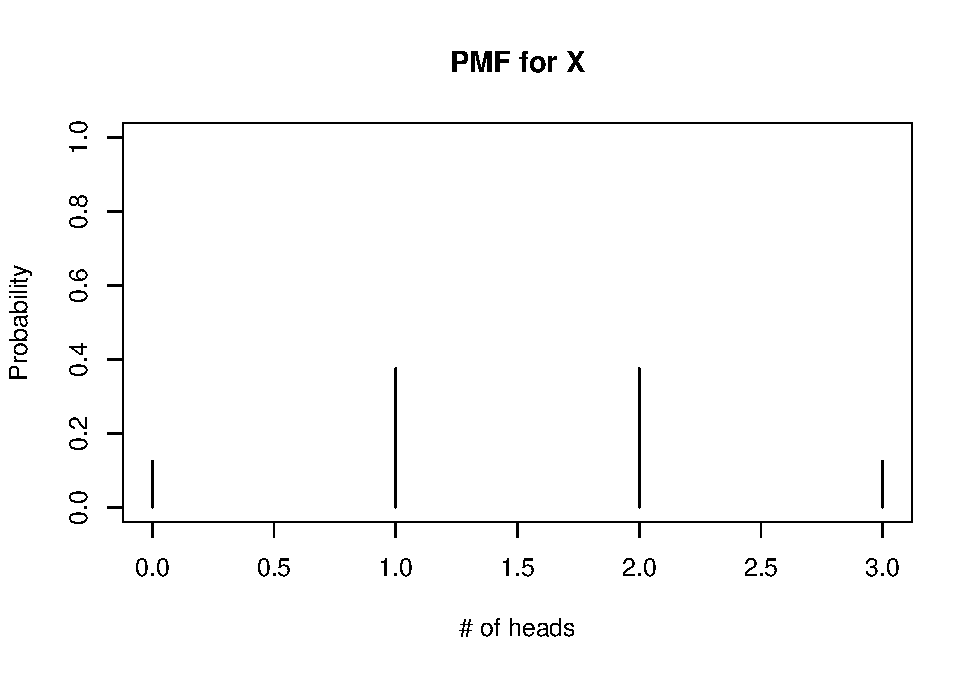
\includegraphics{bookdown-demo_files/figure-latex/3-pmf-1.pdf}
\caption{\label{fig:3-pmf}PMF for X}
\end{figure}

The PMF provides a list of all possible values for the random variable and the corresponding probabilities. In other words, the PMF describes the distribution of the relative frequencies for each outcome. For our experiment, observing 1 or 2 heads is equally likely, and they occur three times as often as observing 0 or 3 heads. Observing 0 or 3 heads is also equally likely.

\subsection{Valid PMFs}\label{valid-pmfs}

Consider a discrete random variable \(X\) with support \(x_1, x_2, \cdots\). The PMF \(P_X(x)\) of \(X\) must satisfy:

\begin{itemize}
\tightlist
\item
  \(P_X(x) > 0\) if \(x = x_j\), and \(P_X(x) = 0\) otherwise.
\item
  \(\sum_{j=1}^{\infty} P_X(x_j) = 1\).
\end{itemize}

In other words, the probabilities associated with the support are greater than 0, and the sum of the probabilities across the whole support must add up to 1.

\emph{Thought question}: based on Table \ref{tab:3-pmf-tab}, can you see why our PMF for \(X\) is valid?

\subsection{PMFs and Histograms}\label{pmfhist}

Recall the frequentist viewpoint of probability, that it represents the relative frequency associated with an event that is repeated for an infinite number of times.

Consider our experiment where we flip a coin 3 times and count the number of heads. The support of our random variable \(X\), the number of heads, is \(\{0,1,2,3 \}\). Imagine performing our experiment a large number of times. Each time we perform the experiment, we record the number of heads. If we performed the experiment one million times, we would have recorded one million values for the number of heads, and each value must be in the support of \(X\). If we then create a histogram for the one million values for the number of heads, the shape of the histogram should be very close to the shape of the plot of the PMF in Figure \ref{fig:3-pmf}. Figure \ref{fig:3-sim} below shows the resulting histogram after performing the experiment 1 million times.

\begin{figure}
\centering
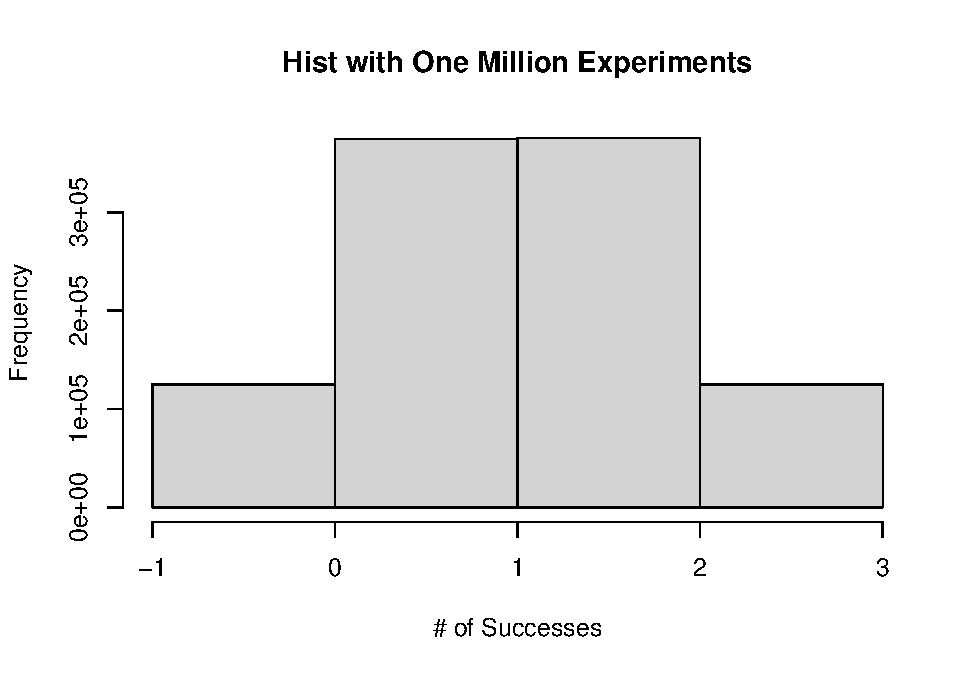
\includegraphics{bookdown-demo_files/figure-latex/3-sim-1.pdf}
\caption{\label{fig:3-sim}Histogram from Experiment Performed 1 Million Times}
\end{figure}

In general, the PMF of a random variable should match the histogram in the long run.

Note: What we have just done here was to use simulations to repeat an experiment a large number of times.

\section{Cumulative Distribution Functions (CDFs)}\label{cumulative-distribution-functions-cdfs}

Another function that is used to describe the distribution of discrete random variables is the \textbf{cumulative distribution function (CDF)}. The CDF of a random variable \(X\) is \(F_X(x) = P(X \leq x)\). Notice that unlike the PMF, the definition of CDF applies for both discrete and continuous random variables.

Going back to our example where we record the number of heads out of 3 coin flips, we can write out the CDF for the random variable \(X\):

\begin{itemize}
\tightlist
\item
  \(F_X(0) = P(X \leq 0) = P(X=0) = \frac{1}{8}\),
\item
  \(F_X(1) = P(X \leq 1) = P(X=0) + P(X=1) = \frac{1}{8} +  \frac{3}{8} = \frac{1}{2}\),
\item
  \(F_X(2) = P(X \leq 2) = P(X=0) + P(X=1) + P(X=2) = \frac{1}{2} + \frac{3}{8} = \frac{7}{8}\),
\item
  \(F_X(3) = P(X \leq 3) = P(X=0) + P(X=1) + P(X=2) + P(X=3) = \frac{7}{8} + \frac{1}{8} = 1\).
\end{itemize}

Notice how these calculations were based on the PMF. To find \(P(X \leq x)\), we summed the PDF over all values of the support that is less than or equal to \(x\). Therefore, another way to write the CDF for a discrete random variable is

\begin{equation} 
F_X(x) = P(X \leq x) = \sum_{x_j \leq x} P(X=x_j).
\label{eq:3-CDF}
\end{equation}

Fairly often, the CDF of a discrete random variable is presented in a simple table like Table \ref{tab:3-cdf-tab} below:

\begin{table}

\caption{\label{tab:3-cdf-tab}CDF for X}
\centering
\begin{tabular}[t]{r|r}
\hline
x & CDF\\
\hline
0 & 0.125\\
\hline
1 & 0.500\\
\hline
2 & 0.875\\
\hline
3 & 1.000\\
\hline
\end{tabular}
\end{table}

Or in a simple plot like in Figure \ref{fig:3-cdf} below:

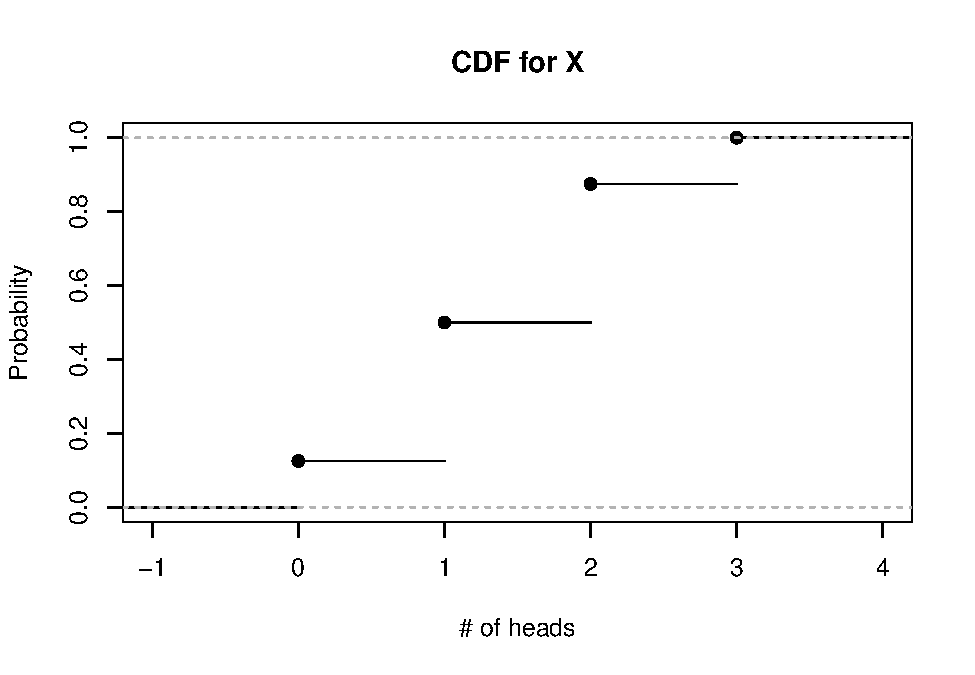
\includegraphics{bookdown-demo_files/figure-latex/3-cdf-1.pdf}
The CDF for discrete random variables always look like a step function, as it increases in discrete jumps at each value of the support. The height of each jump corresponds to the PMF at that value of the support.

\emph{Thought question}: do you see similarities between the CDF and the empirical cumulative density function (ECDF) from section \ref{ecdf}?

\subsection{Valid CDFs}\label{valid-cdfs}

The CDF \(F_X(x)\) of \(X\) must:

\begin{itemize}
\tightlist
\item
  be non decreasing. This means that as \(x\) gets larger, the CDF either stays the same or increases. Visually, a graph of the CDF never decreases as \(x\) increases.
\item
  approach 1 as \(x\) approaches infinity and approach 0 as \(x\) approaches negative infinity. Visually, a graph of the CDF should be equal to or close to 1 for large values of x, and it should be equal to or close to 0 for small values of x.
\end{itemize}

\emph{Thought question}: Look at the CDF for our example in Figure \ref{fig:3-cdf}, and see how it satisfies the criteria listed above for a valid CDF.

\section{Expectations}\label{expectations}

In the previous section, we see how PMFs and CDFs can be used to describe the distribution of a random variable. As the PMF can be viewed as a long-run version of the histogram, it gives us an idea about the shape of the distribution. Similar to Section \ref{descriptive}, we will also be interested in measures of centrality and spread for random variables.

A measure of centrality for random variables is the \textbf{expectation}, or \textbf{expected value}. The expectation of a random variable can be interpreted as the long-run mean of the random variable, i.e.~if we were able to repeat the experiment an infinite number of times, the expectation of the random variable will be the average result among all the experiments.

For a discrete random variable \(X\) with support \(x_1, x_2, \cdots,\), the expected value, denoted by \(E(X)\), is

\begin{equation} 
E(X) = \sum_{j=1}^{\infty} x_j P(X=x_j).
\label{eq:3-EX}
\end{equation}

We can use Table \ref{tab:3-pmf-tab} as an example. To find the expected number of heads out of 3 coin flips, using equation \eqref{eq:3-EX},

\[
\begin{split}
E(X) &= 0 \times \frac{1}{8} + 1 \times \frac{3}{8} + 2 \times \frac{3}{8} + 3 \times \frac{1}{8}\\
       &= 1.5
\end{split}
\]

What we did was to take the product of each value in the support of the random variable with its corresponding probability, and add all these products.

We can see another interpretation of the expected value of a random variable from this calculation: it is the weighted average of the values for the random variable, weighted by their probabilities.

Intuitively, this expected value of 1.5 should make sense. If we flip a coin 3 times, and the coin is fair, we expect half of these flips to land heads, or 1.5 flips to land heads.

View the video below for a more detailed explanation on how to calculate expected values:

\subsection{Linearity of Expectations}\label{linearity-of-expectations}

We have seen how to calculate the expected value of a random variable \(X\) using equation \eqref{eq:3-EX}. What we need is the PMF of \(X\). Sometimes our random variable can be viewed as a sum (or difference) of other random variables, or it could involve a multiplication and / or adding a constant to the random variable. Consider some of these scenarios:

\begin{itemize}
\item
  Suppose my friend and I are fisherman. Let \(Y\) be the random variable describing the number of fish I catch on a workday, and let \(W\) be the random variable describing the number of fish my friend catches on a workday. We can let \(T = Y+W\) be the random variable describing the total number of fish we catch on a workday.
\item
  Suppose that I sell each fish for \$10 and my friend sells each fish for \$15. We can let \(R = 10Y + 15W\) be the random variable that describes the revenue we generate on a workday.
\item
  Suppose that my friend and I rent out a space at the market to sell our fish, and it costs \$5 a day to rent out the space. We can let \(G = 10Y + 15W - 5\) be the random variable that describes our gross income for the day.
\end{itemize}

All of these examples involve new random variables, \(T, R, G\) that can be based on previously defined random variables, \(Y, W\). It turns out that to find the expectations of the new random variables, all we need is the expectations of the previously defined random variables. We do not need to find the PMFs for \(T, R\) and \(S\) and then apply equation \eqref{eq:3-EX}.

These can be done through the \textbf{linearity of expectations}: Let \(X\) and \(Y\) denote random variables, and \(a,b,c\) denote some constants, then

\begin{equation} 
E(aX + bY + c) = aE(X) + bE(Y) + c.
\label{eq:3-linEX}
\end{equation}

Applying equation \eqref{eq:3-linEX} to the fishing examples:

\begin{itemize}
\tightlist
\item
  \(E(T) = R(Y + W) = E(Y) + E(W)\),
\item
  \(E(R) = E(10Y + 15W) = 10E(Y) + 15E(W)\),
\item
  \(E(G) = E(10Y + 15W - 5) = 10E(Y) + 15E(W) - 5\).
\end{itemize}

All we need to find the expected values for the total number of fish, revenue generated, and gross income were the expected values for the number of fish each of us caught. We do not need the PMFs for \(T,R,G\).

\subsubsection{Visual Explanation}\label{visual-explanation}

For a visual explanation of why equation \eqref{eq:3-linEX} makes sense, we go back to our previous example where \(X\) denotes the number of heads in 3 coin flips. Figure \ref{fig:3-pmf} displays the PMF for this random variable. Let us create the PMF for a new random variable \(Y=2X\) and display it in Figure \ref{fig:3-pmf-lin} below:

\begin{Shaded}
\begin{Highlighting}[]
\DocumentationTok{\#\#support of X}
\NormalTok{x}\OtherTok{\textless{}{-}}\DecValTok{0}\SpecialCharTok{:}\DecValTok{3}
\DocumentationTok{\#\# PMF for each value in the support. }
\NormalTok{PMFs}\OtherTok{\textless{}{-}}\FunctionTok{c}\NormalTok{(}\DecValTok{1}\SpecialCharTok{/}\DecValTok{8}\NormalTok{, }\DecValTok{3}\SpecialCharTok{/}\DecValTok{8}\NormalTok{, }\DecValTok{3}\SpecialCharTok{/}\DecValTok{8}\NormalTok{, }\DecValTok{1}\SpecialCharTok{/}\DecValTok{8}\NormalTok{)}
\NormalTok{EX}\OtherTok{\textless{}{-}}\FloatTok{1.5}

\DocumentationTok{\#\#support of Y}
\NormalTok{y}\OtherTok{\textless{}{-}}\DecValTok{2}\SpecialCharTok{*}\NormalTok{x}
\DocumentationTok{\#\# PMF for each value in the support. }
\NormalTok{PMFs}\OtherTok{\textless{}{-}}\FunctionTok{c}\NormalTok{(}\DecValTok{1}\SpecialCharTok{/}\DecValTok{8}\NormalTok{, }\DecValTok{3}\SpecialCharTok{/}\DecValTok{8}\NormalTok{, }\DecValTok{3}\SpecialCharTok{/}\DecValTok{8}\NormalTok{, }\DecValTok{1}\SpecialCharTok{/}\DecValTok{8}\NormalTok{)}
\NormalTok{EY}\OtherTok{\textless{}{-}}\DecValTok{2}\SpecialCharTok{*}\NormalTok{EX}

\FunctionTok{par}\NormalTok{(}\AttributeTok{mfrow=}\FunctionTok{c}\NormalTok{(}\DecValTok{2}\NormalTok{,}\DecValTok{1}\NormalTok{))}

\DocumentationTok{\#\# create plot of PMF vs each value in support}
\FunctionTok{plot}\NormalTok{(x, PMFs, }\AttributeTok{type=}\StringTok{"h"}\NormalTok{, }\AttributeTok{main =} \StringTok{"PMF for X"}\NormalTok{, }\AttributeTok{xlab=}\StringTok{"X"}\NormalTok{, }\AttributeTok{ylab=}\StringTok{"Probability"}\NormalTok{, }\AttributeTok{ylim=}\FunctionTok{c}\NormalTok{(}\DecValTok{0}\NormalTok{,}\DecValTok{1}\NormalTok{))}
\DocumentationTok{\#\#overlay a line representing EX in red}
\FunctionTok{abline}\NormalTok{(}\AttributeTok{v=}\NormalTok{EX, }\AttributeTok{col=}\StringTok{"red"}\NormalTok{)}

\DocumentationTok{\#\# create plot of PMF vs each value in support}
\FunctionTok{plot}\NormalTok{(y, PMFs, }\AttributeTok{type=}\StringTok{"h"}\NormalTok{, }\AttributeTok{main =} \StringTok{"PMF for Y"}\NormalTok{, }\AttributeTok{xlab=}\StringTok{"Y"}\NormalTok{, }\AttributeTok{ylab=}\StringTok{"Probability"}\NormalTok{, }\AttributeTok{ylim=}\FunctionTok{c}\NormalTok{(}\DecValTok{0}\NormalTok{,}\DecValTok{1}\NormalTok{))}
\DocumentationTok{\#\#overlay a line representing EY in red}
\FunctionTok{abline}\NormalTok{(}\AttributeTok{v=}\NormalTok{EY, }\AttributeTok{col=}\StringTok{"red"}\NormalTok{)}
\end{Highlighting}
\end{Shaded}

\begin{figure}
\centering
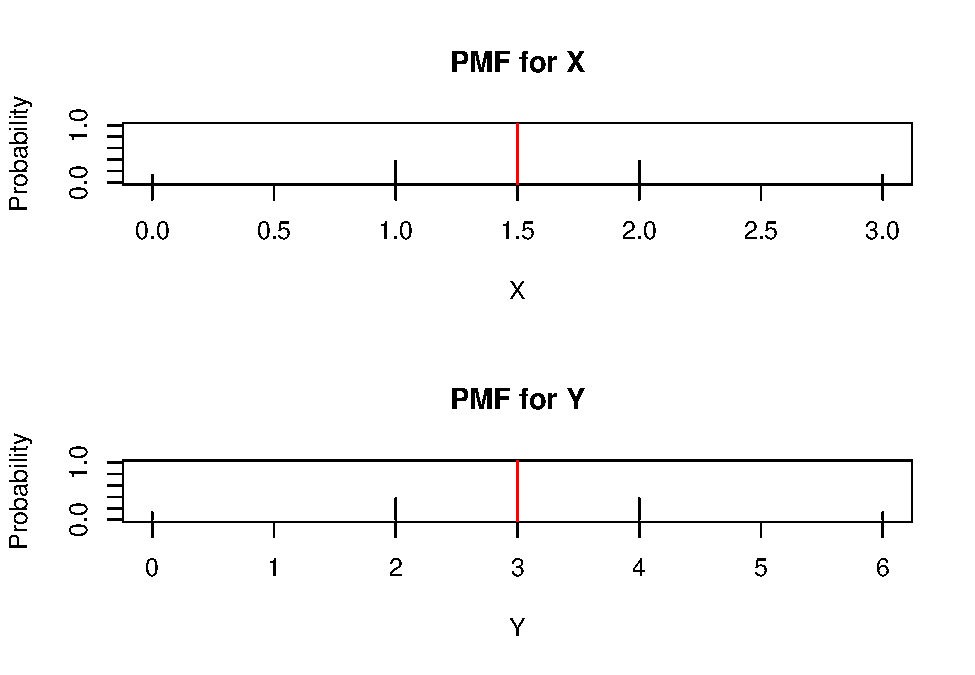
\includegraphics{bookdown-demo_files/figure-latex/3-pmf-lin-1.pdf}
\caption{\label{fig:3-pmf-lin}PMF for X and Y=2X}
\end{figure}

Note that the red vertical lines represent the expected value for the random variable, and since the PMFs are symmetric, the expected value lies right in the middle of the support. Comparing the PMFs in Figure \ref{fig:3-pmf-lin}, we get \(Y\) by multiplying \(X\) by 2. So the support of \(Y\) is now \(\{0,2,4,6\}\) but the associated probabilities are unchanged, so the heights of the probabilities on the vertical axis are unchanged. Therefore, the center, the expected value, is multiplied by the same constant.

Consider another random variable \(W = X+3\). We create the PMF for \(W\) and display it in Figure \ref{fig:3-pmf-lin2} below:

\begin{Shaded}
\begin{Highlighting}[]
\DocumentationTok{\#\#support of X}
\NormalTok{x}\OtherTok{\textless{}{-}}\DecValTok{0}\SpecialCharTok{:}\DecValTok{3}
\DocumentationTok{\#\# PMF for each value in the support. }
\NormalTok{PMFs}\OtherTok{\textless{}{-}}\FunctionTok{c}\NormalTok{(}\DecValTok{1}\SpecialCharTok{/}\DecValTok{8}\NormalTok{, }\DecValTok{3}\SpecialCharTok{/}\DecValTok{8}\NormalTok{, }\DecValTok{3}\SpecialCharTok{/}\DecValTok{8}\NormalTok{, }\DecValTok{1}\SpecialCharTok{/}\DecValTok{8}\NormalTok{)}
\NormalTok{EX}\OtherTok{\textless{}{-}}\FloatTok{1.5}

\DocumentationTok{\#\#support of W}
\NormalTok{w}\OtherTok{\textless{}{-}}\NormalTok{x}\SpecialCharTok{+}\DecValTok{3}
\DocumentationTok{\#\# PMF for each value in the support. }
\NormalTok{PMFs}\OtherTok{\textless{}{-}}\FunctionTok{c}\NormalTok{(}\DecValTok{1}\SpecialCharTok{/}\DecValTok{8}\NormalTok{, }\DecValTok{3}\SpecialCharTok{/}\DecValTok{8}\NormalTok{, }\DecValTok{3}\SpecialCharTok{/}\DecValTok{8}\NormalTok{, }\DecValTok{1}\SpecialCharTok{/}\DecValTok{8}\NormalTok{)}
\NormalTok{EW}\OtherTok{\textless{}{-}}\NormalTok{EX}\SpecialCharTok{+}\DecValTok{3}

\FunctionTok{par}\NormalTok{(}\AttributeTok{mfrow=}\FunctionTok{c}\NormalTok{(}\DecValTok{2}\NormalTok{,}\DecValTok{1}\NormalTok{))}

\DocumentationTok{\#\# create plot of PMF vs each value in support}
\FunctionTok{plot}\NormalTok{(x, PMFs, }\AttributeTok{type=}\StringTok{"h"}\NormalTok{, }\AttributeTok{main =} \StringTok{"PMF for X"}\NormalTok{, }\AttributeTok{xlab=}\StringTok{"X"}\NormalTok{, }\AttributeTok{ylab=}\StringTok{"Probability"}\NormalTok{, }\AttributeTok{ylim=}\FunctionTok{c}\NormalTok{(}\DecValTok{0}\NormalTok{,}\DecValTok{1}\NormalTok{))}
\DocumentationTok{\#\#overlay a line representing EX in red}
\FunctionTok{abline}\NormalTok{(}\AttributeTok{v=}\NormalTok{EX, }\AttributeTok{col=}\StringTok{"red"}\NormalTok{)}

\DocumentationTok{\#\# create plot of PMF vs each value in support}
\FunctionTok{plot}\NormalTok{(w, PMFs, }\AttributeTok{type=}\StringTok{"h"}\NormalTok{, }\AttributeTok{main =} \StringTok{"PMF for w"}\NormalTok{, }\AttributeTok{xlab=}\StringTok{"W"}\NormalTok{, }\AttributeTok{ylab=}\StringTok{"Probability"}\NormalTok{, }\AttributeTok{ylim=}\FunctionTok{c}\NormalTok{(}\DecValTok{0}\NormalTok{,}\DecValTok{1}\NormalTok{))}
\DocumentationTok{\#\#overlay a line representing EW in red}
\FunctionTok{abline}\NormalTok{(}\AttributeTok{v=}\NormalTok{EW, }\AttributeTok{col=}\StringTok{"red"}\NormalTok{)}
\end{Highlighting}
\end{Shaded}

\begin{figure}
\centering
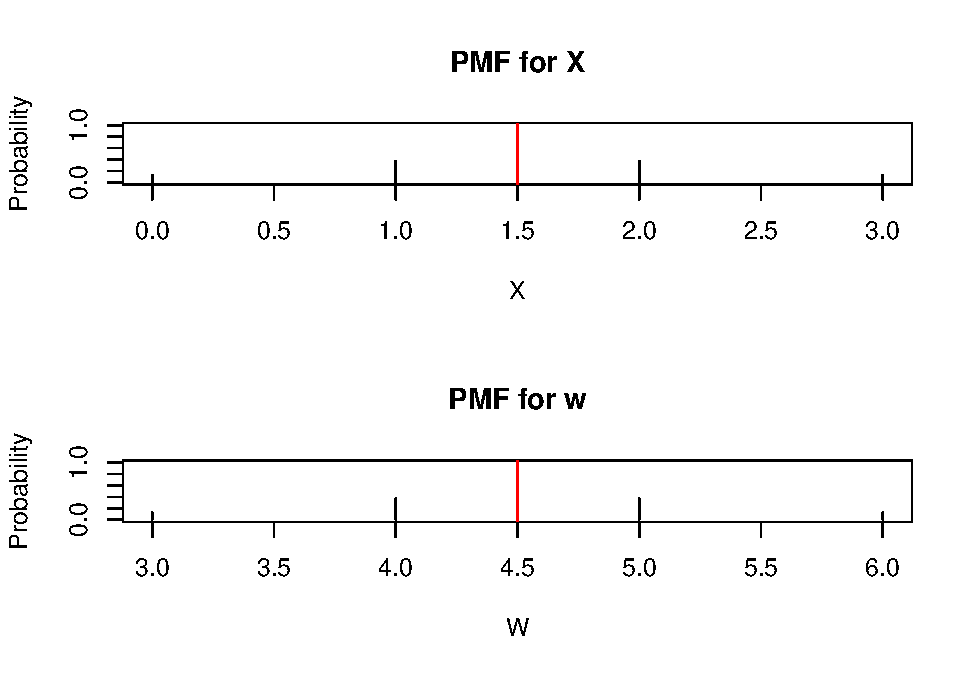
\includegraphics{bookdown-demo_files/figure-latex/3-pmf-lin2-1.pdf}
\caption{\label{fig:3-pmf-lin2}PMF for X and W=X+3}
\end{figure}

Notice the PMFs for \(X\) and \(W\) look almost exactly the same. The only difference is that every value in the support for \(X\) is shifted by 3 units. The probabilities stay the same, so the heights in the PMFs are unchanged. So if every value is shifted by 3 units, the expected value, the long-run average, also gets shifted by 3 units. Adding a constant to a random variable shifts the expected value accordingly.

\subsubsection{One More Example}\label{one-more-example}

We look at one more example to illustrate the usefulness of the linearity of expectations. Consider a drunk man who has to walk on a one-dimensional number line and starts at the 0 position. For each step the drunk man takes, he either moves forward, backward, or stays at the same spot. He steps forward with probability \(p_f\), backward with probability \(p_b\), and stays at the same spot with probability \(p_s\), where \(p_f + p_b+p_s = 1\). Let \(Y\) be the position on the number line of the drunk man after 2 steps. What is the expected position of the drunk man after two steps, i.e.~what is \(E(Y)\)? Assume that each step is independent.

Using brute force, we can find the PMF of \(Y\), and find \(E(Y)\) using equation \eqref{eq:3-EX}. First, we need to find the sample space for \(Y\). With two steps, the sample space is \(\{-2,-1,0,1,2\}\). Next, we need to find the probabilities associated with each outcome in the sample space.

\begin{itemize}
\tightlist
\item
  For \(Y=-2\), the man must move backward on each step. This probability will be \(P(Y=-2) = p_b^2\).
\item
  Likewise, for \(Y=2\), the man must move forward on each step. This probability will be \(P(Y=2) = p_f^2\).
\item
  For \(Y=-1\), the man could stay on the first step, then move back on the second, or move back on the first step, and stay on the second. This probability will be \(P(Y=-1) = p_s p_b + p_b p_s = 2p_b p_s\).
\item
  Likewise, for \(Y=1\), the man could stay on the first step, then move forward on the second, or move forward on the first step, and stay on the second. This probability will be \(P(Y=1) = p_s p_f + p_f p_s = 2p_f p_s\).
\item
  For \(Y=0\), the man could move forward, then backward, or move backward then forward, or stay on both steps. So \(P(Y=0) = p_f p_b + p_b p_f + p_s^2 = p_s^2 + 2 p_b p_f\).
\end{itemize}

Using equation \eqref{eq:3-EX},

\[
\begin{split}
E(Y) &= -2 \times p_b^2 + -1 \times 2p_b p_s + 0 \times p_s^2 + 2 p_b p_f + 1 \times 2p_f p_s + 2 \times p_f^2 \\
       &= 2 (p_f - p_b)
\end{split}
\]

Note: I skipped a lot of messy algebra to get to the end result. Even with skipping some of the messy algebra, setting up the PMF was quite a bit of work.

Suppose we use the linearity of expectations in equation \eqref{eq:3-linEX}. Let \(Y_1, Y_2\) denote the distance the man moves at step 1 and 2 respectively. Then \(Y = Y_1 + Y_2\). The sample of \(Y_1\) and \(Y_2\) are the same: \(\{-1,0,1\}\). Both \(Y_1\) and \(Y_2\) have the following PMF:

\begin{itemize}
\tightlist
\item
  \(P(Y_i = -1) = p_b\)
\item
  \(P(Y_i = 0) = p_s\)
\item
  \(P(Y_i = 1) = p_f\)
\end{itemize}

And using equation \eqref{eq:3-EX},

\[
\begin{split}
E(Y_i) &= -1 \times p_b + 0 \times p_s + 1 \times p_f \\
       &= p_f - p_b
\end{split}
\]

So therefore \(E(Y) = E(Y_1 + Y_2) = E(Y_1) + E(Y_2) = 2(p_f - p_b)\). Both approaches resulted in the same answer, but notice how much simpler its was to obtain the solution using linearity of expectations. Imagine if we wanted to find the expected position after 500 steps? Writing out the sample space for 500 steps will be extremely long.

View the video below for a more detailed explanation of this worked example:

\subsection{Law of the Unconscious Statistician}\label{law-of-the-unconscious-statistician}

Suppose we have the PMF of a random variable \(X\), and we want to find \(E(g(X))\), where \(g\) is a function of \(X\) (you can think of \(g\) as a transformation performed on \(X\)). One idea could be to find the PMF of \(g(X)\) and then use the definition of expectation in equation \eqref{eq:3-EX}. But we have seen in the previous subsection that finding the sample space after transforming the random variable can be challenging. It turns out we can find \(E(g(X))\) based on the PMF of \(X\), without having to find the PMF of \(g(X)\).

This is done through the \textbf{Law of the Unconscious Statistician (LOTUS)}. Let \(X\) be a discrete random variable with support \(\{x_1, x_2, \cdots \}\), and \(g\) is a function applied to \(X\), then

\begin{equation} 
E(g(X)) = \sum_{i=j}^{\infty} g(x_j) P(X=x_j).
\label{eq:3-lotus}
\end{equation}

An application of LOTUS is in finding the variance of a discrete random variable.

\subsection{Variance}\label{variance}

We have talked about the shape of the distribution of a discrete random variable, and its expected value. One more measure that we are interested in is the spread associated with the distribution. One common measure is the variance of the random variable.

The \textbf{variance} of a random variable \(X\) is

\begin{equation} 
Var(X) = E[(X - EX)^2]
\label{eq:3-var2}
\end{equation}

and the \textbf{standard deviation} of a random variable \(X\) is the square root of its variance

\begin{equation} 
SD(X) = \sqrt{Var(X)}.
\label{eq:3-sd}
\end{equation}

Looking at equation \eqref{eq:3-var2} a little more closely, we can see a natural interpretation of the variance of a random variable: it is the average squared distance of the random variable from its mean, in the long-run. An equivalent formula for the variance of a random variable is

\begin{equation} 
Var(X) = E(X^2) - (EX)^2.
\label{eq:3-var}
\end{equation}

Equation \eqref{eq:3-var} is easier to work with than equation \eqref{eq:3-var2} when performing actual calculations.

Let us now go back to our original example, where \(X\) denotes the number of heads out of 3 coin flips. Earlier, we found the PMF of this random variable, per Table \ref{tab:3-pmf-tab}, and we found its expectation to be 1.5. To find the variance of \(X\) using equation \eqref{eq:3-var}, we find \(E(X^2)\) first using LOTUS in equation \eqref{eq:3-lotus}

\[
\begin{split}
E(X^2) &= 0^2 \times \frac{1}{8} + 1^2 \times \frac{3}{8} + 2^2 \times \frac{3}{8} + 3^2 \times \frac{1}{8} \\
       &= 3
\end{split}
\]

so \(Var(x) = 3 - 1.5^2 = \frac{3}{4}\).

\emph{Thought question}: Try to find \(Var(X)\) using equation \eqref{eq:3-var2} and LOTUS. You should arrive at the same answer but the steps may be a bit more complicated.

View the video below for a more detailed explanation on how to calculate variance of discrete random variables using equations \eqref{eq:3-var} and \eqref{eq:3-var2}:

\subsubsection{Properties of Variance}\label{var-prop}

Variance has the following properties:

\begin{itemize}
\tightlist
\item
  \(Var(X+c) = Var(X)\), where \(c\) is a constant. This should make sense, since if we add a constant to a random variable, we shift it by \(c\) units. As shown earlier in Figure \ref{fig:3-pmf-lin2}, the expected value also gets shifted by \(c\) units. Variance measures the average squared distance of a variable from its mean. So the distance, and the squared distance, of \(X\) from its mean is unchanged.
\item
  \(Var(cX) = c^2 Var(X)\). Look at Figure \ref{fig:3-pmf-lin}, notice the distance between each value in the support from its expected value gets multiplied by 2 (since \(Y=2X\)). So if we multiply a random variable by \(c\), the distance between each value in the support on its expected value is multiplied by \(c\). Since variance measures squared distance, the variance gets multiplied by \(c^2\).
\item
  If \(X\) and \(Y\) are independent random variables, then \(Var(X+Y) = Var(X) + Var(Y)\).
\end{itemize}

\section{Common Discrete Random Variables}\label{common-discrete-random-variables}

Next, we will introduce some commonly used distributions that may be used for discrete random variables. A number of common statistical models (for example, logistic regression, Poisson regression) are based on these distributions.

\subsection{Bernoulli}\label{bernoulli}

The Bernoulli distribution might be the simplest discrete random variable. The support for such a random variable is \(\{0,1\}\). In other words, the value of a random variable that follows a Bernoulli distribution is either 0 or 1. A Bernoulli distribution is also described by the parameter \(p\), which is the probability that the random variable takes on the value of 1.

More formally, a random variable \(X\) follows a \textbf{Bernoulli distribution} with parameter \(p\) if \(P(X=1) = p\) and \(P(X=0) = 1-p\), where \(0<p<1\). Using mathematical notation, we can write \(X \sim Bern(p)\) to express that the random variable \(X\) is distributed as a Bernoulli with parameter \(p\). The PMF of a Bernoulli distribution is written as

\begin{equation} 
P(X=k) = p^k (1-p)^{1-k}
\label{eq:3-bern}
\end{equation}

for \(k=0, 1\).

It is not enough to specify that a random variable follows a Bernoulli distribution. We need to also clearly specify the value of the parameter \(p\). Consider the following two examples which describe two different experiments:

\begin{itemize}
\item
  Suppose I flip a fair coin once. Let \(Y=1\) if the coin lands heads, and \(Y=0\) if the coin lands tails. \(Y \sim Bern(\frac{1}{2})\) in this example since the coin is fair.
\item
  Suppose I am asked a question and I am given 5 multiple choices, of which only 1 is the correct answer. I have no idea about the topic, and the multiple choices do not help, so I have to guess. Let \(W=1\) if I answer correctly, and \(W=0\) if I answer incorrectly. \(W \sim Bern(\frac{1}{5})\).
\end{itemize}

\(P(Y=1)\) and \(P(W=1)\) are not the same in these examples.

Fairly often, when we have a Bernoulli random variable, the event that results in the random variable being coded as 1 is called a \textbf{success}, and the event that results in the random variable being coded as 0 is called a \textbf{failure}. In such a setting, the parameter \(p\) is called the \textbf{success probability} of the Bernoulli distribution. An experiment that has a Bernoulli distribution can be called a Bernoulli trial.

If you go back to the second example in section \ref{eg2}, we were modeling whether a job applicant receives a callback or not. In this example, we could let \(V\) be the random variable that an applicant receives a callback, with \(V=1\) denoting the applicant received a callback, and \(V=0\) when the applicant did not receive a callback. We used logistic regression in the example. It turns out that logistic regression is used when the variable of interest follows a Bernoulli distribution.

\subsubsection{Properties of Bernoulli}\label{bernprop}

Consider \(X\) is a Bernoulli distribution with parameter \(p\). The expectation of a Bernoulli distribution is

\begin{equation} 
E(X) = p
\label{eq:3-bern-EX}
\end{equation}

and its variance is

\begin{equation} 
Var(X) = p(1-p).
\label{eq:3-bern-var}
\end{equation}

\emph{Thought question}: Use the definition of expectations for discrete random variables, equation \eqref{eq:3-EX}, and the PMF of a Bernoulli random variable, and LOTUS to prove equations \eqref{eq:3-bern-EX} and \eqref{eq:3-bern-var}.

The expected value being equal to \(p\) for a Bernoulli distribution should make sense. Remember that the support for such a random variable is 0 or 1, with \(P(X=1) = p\). Using the frequentist viewpoint, if we were to flip a coin and record heads or tails, and repeat this coin flipping many times, we will have record a bunch of 0s and 1s to represent the result for all the coin flips. The average of this bunch of 0s and 1s is just the proportion of 1s.

The equation for the variance of a Bernoulli distribution exhibits an interesting and intuitive behavior. Figure \ref{fig:3-varBern} below shows how the variance behaves as we vary the value of \(p\):

\begin{Shaded}
\begin{Highlighting}[]
\NormalTok{p}\OtherTok{\textless{}{-}}\FunctionTok{seq}\NormalTok{(}\DecValTok{0}\NormalTok{,}\DecValTok{1}\NormalTok{,}\AttributeTok{by =} \FloatTok{0.001}\NormalTok{) }\DocumentationTok{\#\#sequence of values for p}
\NormalTok{Bern\_var}\OtherTok{\textless{}{-}}\NormalTok{p}\SpecialCharTok{*}\NormalTok{(}\DecValTok{1}\SpecialCharTok{{-}}\NormalTok{p) }\DocumentationTok{\#\#variance of Bernoulli}
\DocumentationTok{\#\#plot variance against p}
\FunctionTok{plot}\NormalTok{(p, Bern\_var, }\AttributeTok{ylab=}\StringTok{"Variance"}\NormalTok{, }\AttributeTok{main=}\StringTok{"Variance of Bernoulli as p is Varied"}\NormalTok{)}
\end{Highlighting}
\end{Shaded}

\begin{figure}
\centering
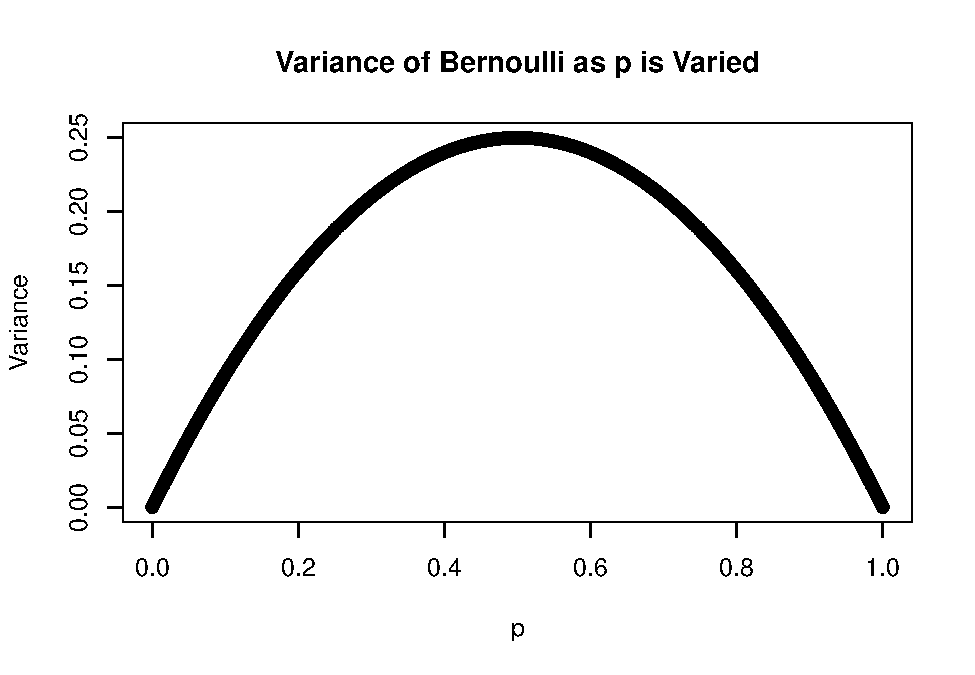
\includegraphics{bookdown-demo_files/figure-latex/3-varBern-1.pdf}
\caption{\label{fig:3-varBern}Variance of Bernoulli}
\end{figure}

Notice the variance is at a maximum when \(p=0.5\), and the variance is minimum (in fact it is 0) when \(p=0\) or \(p=1\). If we have a biased coin such that it always lands heads, every coin flip will land on heads with no exception. There is no variability in the result, and we have utmost certainty in the result of each coin flip. On the other hand, if the coin is fair such that \(p=0.5\), we have the least certainty in the result of each coin flip, and so variance is maximum when the coin is fair.

Another application of this property is during election results (assuming 2 candidates, but the same idea applies for more candidates). For swing states where the race is closer (so \(p\) is closer to half), projections on the winner have more uncertainty and so we need to get more data and wait longer for the projections. For states that primarily vote for one candidate (so \(p\) is closer to 0 or 1), projections happen a lot quicker as projections have less uncertainty.

\subsection{Binomial}\label{binomial}

Suppose we have an experiment that follows a Bernoulli distribution, and we perform this experiment \(n\) times (sometimes called trials), each time with the same success probability \(p\). The experiments are independent from each other. Let \(X\) denote the number of successes out of the \(n\) trials. \(X\) follows a \textbf{binomial distribution} with parameters \(n\) and \(p\) (number of trials and success probability). We write \(X \sim Bin(n,p)\) to express that \(X\) follows a binomial distribution with parameters \(n\) and \(p\), with \(n>0\) and \(0<p<1\). The PMF of a Binomial distribution is written as

\begin{equation} 
P(X=k) = \binom{n}{k} p^k (1-p)^{n-k}
\label{eq:3-bin}
\end{equation}

for \(k=0,1,2, \cdots, n\), which is also the support of the binomial distribution.

In equation \eqref{eq:3-bin}, \(\binom{n}{k}\) is called the binomial coefficient, and it is the number of combinations that result in \(k\) successes out of the \(n\) trials. The binomial coefficient can be found using

\begin{equation} 
\binom{n}{k} =  \frac{n!}{k! (n-k)!}.
\label{eq:3-bincoeff}
\end{equation}

\(n!\) is called n-factorial, and is the product of all positive integers less than or equal to n.~So \(n! = n \times (n-1) \times (n-2) \times \cdots \times 1.\) As an example \(5! = 5 \times 4 \times 3 \times 2 \times 1 = 120\), or using R:

\begin{Shaded}
\begin{Highlighting}[]
\FunctionTok{factorial}\NormalTok{(}\DecValTok{5}\NormalTok{)}
\end{Highlighting}
\end{Shaded}

\begin{verbatim}
## [1] 120
\end{verbatim}

Note: A fairly common model, the logistic regression model with aggregated data, is based on the binomial distribution. We mentioned logistic regression earlier. The difference between these two (with and without aggregated data) is based on the structure of the data frame. If you are interested in these differences, please read \url{https://www.r-bloggers.com/2021/02/how-to-run-logistic-regression-on-aggregate-data-in-r/}.

We go back to our first example of counting the number of heads out of three coin flips follows a binomial distribution.

\begin{itemize}
\tightlist
\item
  Each coin flip is either heads or tails. There are only two outcomes for each flip.
\item
  The success probability, the probability of heads, is 0.5 and is the same for each flip. The parameter is fixed for each flip.
\item
  The result of each flip is independent of other flips since other flips do not affect the outcome.
\item
  The number of trials (flips in this example) is \(n=3\) is specified as a fixed value.
\end{itemize}

Since these four conditions are met, the number of heads in 3 coin flips can be modeled using a binomial distribution. We let \(x\) denote the number of heads in 3 coin clips, so we write \(X \sim Bin(3,0.5)\).

Suppose we want to calculate \(P(X=2)\) using equation \eqref{eq:3-bin}:

\[
\begin{split}
P(X=2) &= \binom{3}{2} (0.5)^2 (0.5)^1\\
       &= \frac{3!}{2! 1!} (0.5)^2 (0.5)^1 \\
       &= 3 \times \frac{1}{8} \\
       &= \frac{3}{8}.
\end{split}
\]

In this example, the binomial coefficient equals to 3. Which indicates there were 3 combinations to obtain 2 heads in 3 coin flips. \(P(X=2)\) can be written as \(P(HHT \cup HTH \cup THH)\). Solving for \(P(HHT \cup HTH \cup THH)\), we have

\[
\begin{split}
P(HHT \cup HTH \cup THH) &= P(HHT) + P(HTH) + P(THH)\\
       &= 0.5^3 + 0.5^3 + 0.5^3 \\
       &= 3 \times \frac{1}{8} \\
       &= \frac{3}{8}.
\end{split}
\]
so we could have solved this using basic probability rules from the previous module, without using the PMF of the binomial distribution in equation \eqref{eq:3-bin}. Of course, the PMF of the binomial distribution gets a lot more convenient if \(n\) gets larger, as the number of combinations and sample space get a lot larger.

We can also use R to find \(P(X=2)\):

\begin{Shaded}
\begin{Highlighting}[]
\FunctionTok{dbinom}\NormalTok{(}\DecValTok{2}\NormalTok{,}\DecValTok{3}\NormalTok{,}\FloatTok{0.5}\NormalTok{) }\DocumentationTok{\#\#specify values of k, n, p in this order}
\end{Highlighting}
\end{Shaded}

\begin{verbatim}
## [1] 0.375
\end{verbatim}

\subsubsection{Relationship Between Binomial and Bernoulli}\label{relationship-between-binomial-and-bernoulli}

Looking at the description of the Bernoulli and binomial distributions, you may notice that a Bernoulli random variable is a special case of a binomial random variable when \(n=1\), i.e.~when we have only 1 trial.

The binomial random variable is also sometimes viewed as the sum of \(n\) independent Bernoulli random variables, all with the same value of \(p\).

\subsubsection{Properties of Binomial}\label{properties-of-binomial}

If \(X \sim Bin(n,p)\), then

\begin{equation} 
E(X) = np
\label{eq:3-bin-EX}
\end{equation}

and

\begin{equation} 
Var(X) = np(1-p).
\label{eq:3-bin-var}
\end{equation}

These results should make sense when we note the relationship between a binomial random variable and Bernoulli random variable. Suppose we have random variables \(Y_1, Y_2, \cdots, Y_n\) and they are all Bernoulli random variables with parameter \(p\) and are independent. Then \(Y = Y_1 + Y_2 + \cdots + Y_n \sim Bin(n,p)\). Therefore, using the linearity of expectations in equation \eqref{eq:3-linEX}, \(E(Y) = E(Y_1) + E(Y_2) + \cdots + E(Y_n) = np\). Since \(Y_1, Y_2, \cdots, Y_n\) are independent, \(Var(Y) = Var(Y_1) + Var(Y_2) + \cdots + Var(Y_n) = np(1-p)\).

\subsubsection{PMFs of Binomial}\label{pmfs-of-binomial}

We take a look at the PMFs of a few binomials, all with \(n=10\) but we vary \(p\) to be 0.2, 0.5, and 0.9, in Figure \ref{fig:3-pmfs}:

\begin{figure}
\centering
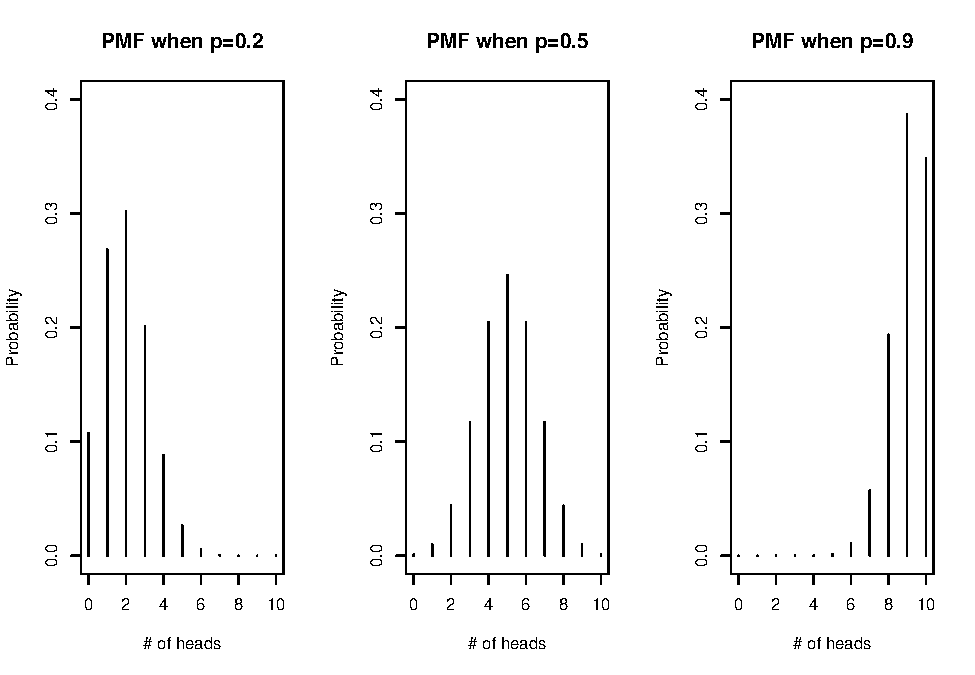
\includegraphics{bookdown-demo_files/figure-latex/3-pmfs-1.pdf}
\caption{\label{fig:3-pmfs}PMF for X, n=10, p varied}
\end{figure}

From figure \ref{fig:3-pmfs}, we can see that the distribution of the binomial is symmetric when \(p=0.5\), as middle values of \(k\) have higher probabilities, and the probabilities decrease as we go further away from the middle. When \(p \neq 0.5\), we see that the distribution gets skewed. When the success probability is small, smaller number of successes are likelier, and when the success probability is large, larger number of successes are likelier, which is intuitive. If the probability of success is small, we expect most outcomes to be failures.

\subsection{Poisson}\label{poisson}

One more common distribution used for discrete random variables is the Poisson distribution. This is often used when the variable of interest is what we call count data (the support is non negative integers), for example, the number of cars that cross an intersection during the day.

A random variable \(X\) follows a \textbf{Poisson distribution} with parameter \(\lambda\), where \(\lambda>0\). Using mathematical notation, we can write \(X \sim Pois(\lambda)\) to express that the random variable \(X\) is distributed as a Poisson with parameter \(p\). The PMF of a Poisson distribution is written as

\begin{equation} 
P(X=k) = \frac{e^{-\lambda}\lambda^k}{k!} 
\label{eq:3-pois}
\end{equation}

for \(k=0,1,2,\cdots\). \(\lambda\) is sometimes called a rate parameter, as it is related to the rate of arrivals, for example, the number of that cross an intersection during a period of time.

\subsubsection{Properties of Poisson}\label{properties-of-poisson}

If \(X \sim Pois(\lambda)\), then

\begin{equation} 
E(X) = \lambda
\label{eq:3-pois-EX}
\end{equation}

and

\begin{equation} 
Var(X) = \lambda.
\label{eq:3-pois-var}
\end{equation}

These imply that larger values of a Poisson random variable are associated with larger variances. This is a common feature for count data. Consider the number of cars that cross an intersection during a one-hour time period. Consider the average number of cars during rush hour, say between 5 and 6pm. This average number is large, but the number could be a lot smaller due to inclement weather, or the number could get a lot larger is there is a convention occurring nearby. On the other hand, consider the average number of cars between 3 and 4am. This average number is small, and is likely to be small all the time, regardless of weather conditions and whether special events are happening.

Another interesting property of the Poisson distribution is that it is skewed when \(\lambda\) is small, and approaches a bell-shaped distribution as \(\lambda\) gets bigger. Figure \ref{fig:3-pmfs-lambda} displays density plots of Poisson distributions as \(\lambda\) is varied:

\begin{Shaded}
\begin{Highlighting}[]
\DocumentationTok{\#\#calculate probability of Poisson with these values on the support}
\NormalTok{x}\OtherTok{\textless{}{-}}\DecValTok{0}\SpecialCharTok{:}\DecValTok{20}
\NormalTok{lambda}\OtherTok{\textless{}{-}}\FunctionTok{c}\NormalTok{(}\FloatTok{0.5}\NormalTok{, }\DecValTok{1}\NormalTok{, }\DecValTok{4}\NormalTok{, }\DecValTok{10}\NormalTok{) }\DocumentationTok{\#\#try 4 different values of lambda}

\DocumentationTok{\#\#create PMFs of these 4 Poissons with different lambdas}
\FunctionTok{par}\NormalTok{(}\AttributeTok{mfrow=}\FunctionTok{c}\NormalTok{(}\DecValTok{2}\NormalTok{,}\DecValTok{2}\NormalTok{))}
\ControlFlowTok{for}\NormalTok{ (i }\ControlFlowTok{in} \DecValTok{1}\SpecialCharTok{:}\DecValTok{4}\NormalTok{)}
  
\NormalTok{\{}
\NormalTok{  dens}\OtherTok{\textless{}{-}}\FunctionTok{dpois}\NormalTok{(x,lambda[i])}
  \FunctionTok{plot}\NormalTok{(x, dens, }\AttributeTok{type=}\StringTok{"l"}\NormalTok{, }\AttributeTok{main=}\FunctionTok{paste}\NormalTok{(}\StringTok{"Lambda is"}\NormalTok{, lambda[i]))}
\NormalTok{\}}
\end{Highlighting}
\end{Shaded}

\begin{figure}
\centering
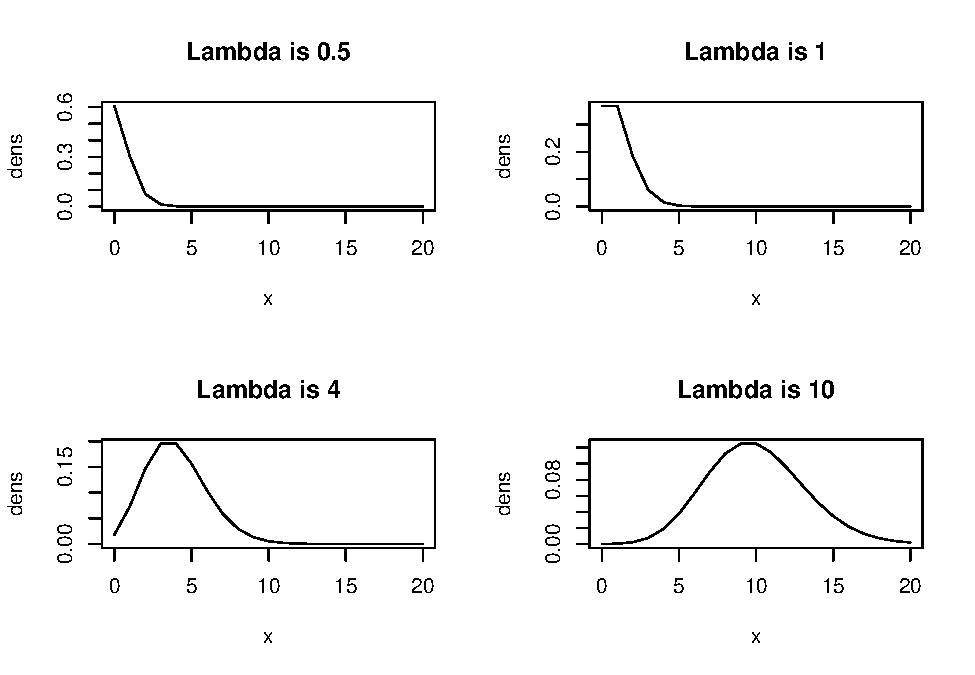
\includegraphics{bookdown-demo_files/figure-latex/3-pmfs-lambda-1.pdf}
\caption{\label{fig:3-pmfs-lambda}PMF for Poissons as Rate Parameter is Varied}
\end{figure}

\subsubsection{Poisson Approximation to Binomial}\label{poisson-approximation-to-binomial}

If \(X \sim Bin(n,p)\), and if \(n\) is large and \(p\) is small, then the PMF of \(X\) can be approximated by a Poisson distribution with rate parameter \(\lambda = np\). In other words, the approximation works better as \(n\) gets larger and \(np\) gets smaller.

There are several rules of thumbs that exist to guide as to how large \(n\) should be and how small \(np\) should be. The National Institute of Standards and Technology \href{https://www.itl.nist.gov/div898/handbook/pmc/section3/pmc331.htm}{(NIST)} suggest \(n \geq 20\) and \(p \leq 0.05\), or \(n \geq 100\), and \(np \leq 10\).

One of the main for using this approximation, instead of directly using the binomial distribution, is that the binomial coefficient can become computationally expensive to compute when \(n\) is large.

Consider this example: A company manufactures computer chips, and 2 percent of chips are defective. The quality control manager randomly samples 100 chips coming off the assembly line. What is the probability that at most 3 chips are defective?

Let \(Y\) denote the number of chips that are defective out of 100 chips.

\begin{itemize}
\tightlist
\item
  Each chip is either defective or not. There are only two outcomes for each chip.
\item
  The ``success'' probability is 0.02 for each chip. This probability is assumed to be fixed for each chip.
\item
  We have to assume that each chip is independent.
\item
  The number of chips is fixed at \(n=100\).
\end{itemize}

So we can model \(Y \sim Bin(100,0.02)\), as long as we assume the chips the independent. To find \(P(Y \leq 3)\), we can:

\begin{itemize}
\tightlist
\item
  use the binomial distribution, or
\item
  approximate it using \(Pois(2)\), as \(\lambda = np = 100 \times 0.02\).
\end{itemize}

\begin{Shaded}
\begin{Highlighting}[]
\DocumentationTok{\#\#set up binomial}
\NormalTok{n}\OtherTok{\textless{}{-}}\DecValTok{100} 
\NormalTok{p}\OtherTok{\textless{}{-}}\FloatTok{0.02} 
\NormalTok{y}\OtherTok{\textless{}{-}}\DecValTok{0}\SpecialCharTok{:}\DecValTok{3} \DocumentationTok{\#\#we want P(Y=0), P(Y=1), P(Y=2), P(Y=3)}
\FunctionTok{sum}\NormalTok{(}\FunctionTok{dbinom}\NormalTok{(y,n,p))}
\end{Highlighting}
\end{Shaded}

\begin{verbatim}
## [1] 0.8589616
\end{verbatim}

\begin{Shaded}
\begin{Highlighting}[]
\DocumentationTok{\#\#Use Poisson to approx binomial}
\NormalTok{lambda}\OtherTok{\textless{}{-}}\NormalTok{n}\SpecialCharTok{*}\NormalTok{p}
\FunctionTok{sum}\NormalTok{(}\FunctionTok{dpois}\NormalTok{(y,lambda))}
\end{Highlighting}
\end{Shaded}

\begin{verbatim}
## [1] 0.8571235
\end{verbatim}

Notice the values are very close to each other.

\section{Using R}\label{Rdis}

R has built in functions to compute the PMF, CDF, percentiles, as well as simulate data of common distributions. We will start using a random variable \(Y\) which follows binomial distribution, with \(n=5, p = 0.3\) as an example first. Note in this example that the support for \(Y\) is \(\{0,1,2,3,4,5 \}\).

\begin{enumerate}
\def\labelenumi{\arabic{enumi}.}
\tightlist
\item
  To find \(P(Y=2)\), use:
\end{enumerate}

\begin{Shaded}
\begin{Highlighting}[]
\FunctionTok{dbinom}\NormalTok{(}\DecValTok{2}\NormalTok{, }\DecValTok{5}\NormalTok{, }\FloatTok{0.3}\NormalTok{) }\DocumentationTok{\#\#supply the value of Y you want, then the parameters n and p in this order}
\end{Highlighting}
\end{Shaded}

\begin{verbatim}
## [1] 0.3087
\end{verbatim}

The probability that \(Y\) is equal to 2 is 0.3087.

\begin{enumerate}
\def\labelenumi{\arabic{enumi}.}
\setcounter{enumi}{1}
\tightlist
\item
  To find \(P(Y \leq 2)\), use:
\end{enumerate}

\begin{Shaded}
\begin{Highlighting}[]
\FunctionTok{pbinom}\NormalTok{(}\DecValTok{2}\NormalTok{, }\DecValTok{5}\NormalTok{, }\FloatTok{0.3}\NormalTok{) }\DocumentationTok{\#\#supply the value of Y you want, then the parameters n and p in this order}
\end{Highlighting}
\end{Shaded}

\begin{verbatim}
## [1] 0.83692
\end{verbatim}

The probability that \(Y\) is less than or equal to 2 is 0.83692.

\begin{enumerate}
\def\labelenumi{\arabic{enumi}.}
\setcounter{enumi}{2}
\tightlist
\item
  To find the value on the support that corresponds to the median (or 50th percentile), use:
\end{enumerate}

\begin{Shaded}
\begin{Highlighting}[]
\FunctionTok{qbinom}\NormalTok{(}\FloatTok{0.5}\NormalTok{, }\DecValTok{5}\NormalTok{, }\FloatTok{0.3}\NormalTok{) }\DocumentationTok{\#\#supply the value of the percentile you need, then the parameters n and p in this order}
\end{Highlighting}
\end{Shaded}

\begin{verbatim}
## [1] 1
\end{verbatim}

The median of a binomial distribution with 5 trials and success probability 0.3 is 1.

\begin{enumerate}
\def\labelenumi{\arabic{enumi}.}
\setcounter{enumi}{3}
\tightlist
\item
  To simulate 10 realizations (replications) of \(Y\), use:
\end{enumerate}

\begin{Shaded}
\begin{Highlighting}[]
\FunctionTok{set.seed}\NormalTok{(}\DecValTok{2}\NormalTok{) }\DocumentationTok{\#\#use set.seed() so we get the same random numbers each time the code is run}
\FunctionTok{rbinom}\NormalTok{(}\DecValTok{10}\NormalTok{, }\DecValTok{5}\NormalTok{, }\FloatTok{0.3}\NormalTok{) }\DocumentationTok{\#\#supply the number of simulated data you need, then the parameters n and p}
\end{Highlighting}
\end{Shaded}

\begin{verbatim}
##  [1] 1 2 2 0 3 3 0 2 1 2
\end{verbatim}

This outputs a vector of length 10. Each value represents the result of each rep. So the first time we ran the binomial distribution with \(n=5, p=0.3\), only 1 out of the 5 was a success. The second time it was run, only 2 out of the 5 was a success, and so on.

Notice these functions all ended with \texttt{binom}. We just added a different letter first, depending on whether we want the PMF, CDF, percentile, or random draw. The letters are \texttt{d}, \texttt{p}, \texttt{q}, and \texttt{r} respectively.

The same idea works for any other distribution. For example, to find the probability of a Poisson distribution with rate parameter 2 being equal to 1, we type:

\begin{Shaded}
\begin{Highlighting}[]
\FunctionTok{dpois}\NormalTok{(}\DecValTok{1}\NormalTok{, }\DecValTok{2}\NormalTok{) }\DocumentationTok{\#\#supply value of k, then parameter}
\end{Highlighting}
\end{Shaded}

\begin{verbatim}
## [1] 0.2706706
\end{verbatim}

\emph{Thought questions:} Suppose \(Y \sim Pois(1)\).

\begin{itemize}
\tightlist
\item
  Find \(P(Y \leq 2)\).
\item
  Find the 75th percentile of \(Y\).
\item
  Simulate 10,000 reps from Y, and find its sample mean. Is the sample mean close to the expected value?
\end{itemize}

\chapter{Continuous Random Variables}\label{continuous-random-variables}

This module is based on Introduction to Probability (Blitzstein, Hwang), Chapters 5 and 6. You can access the book for free at \url{https://stat110.hsites.harvard.edu/} (and then click on Book). Please note that I cover additional topics, and skip certain topics from the book. You may skip Examples 5.1.6, 5.1.7, Proposition 5.2.3, Example 5.2.4, Sections 5.2.6, 5.2.7, Definition 5.3.7, Theorem 5.3.8, Example 5.4.7, Sections 5.5, 5.6, 5.7, Proposition 6.2.5, 6.2.6, Theorem 6.3.4, Sections 6.4 to 6.7 from the book.

\section{Introduction}\label{introduction}

In the previous module, we learned about discrete random variables. We learned how their distributions can be described by the PMFs and CDFs, how to find their expected values and variances, as well as common distributions for discrete random variables. We will learn about their counterparts when dealing with continuous random variables. The concepts are similar, but how they are computed can be quite different.

As a reminder:

\begin{itemize}
\tightlist
\item
  A \textbf{discrete random variable} can only take on a countable (finite or infinite) number of values.
\item
  A \textbf{continuous random variable} can take on an uncountable number of values in an interval of real numbers.
\end{itemize}

For example, height of an American adult is a continuous random variable, as height can take on any value in interval between 40 and 100 inches. All values between 40 and 100 are possible. We cannot list all possible real numbers in this range as the list is never ending.

The sample space associated with a continuous random variable will be difficult to list, since it takes on an uncountable number of values. Using the example of heights of American adults, any real number between 40 and 100 inches is possible.

This is different from a discrete random variable where we would list the sample space, or support, and then find the probability associated with each value in the support.

Similar to discrete random variables, we want to describe the shape of the distribution, the centrality, and the spread of a continuous random distribution so we have an idea of probabilities associated with different ranges of values of the random variable.

\section{Cumulative Distribution Functions (CDFs)}\label{cumulative-distribution-functions-cdfs-1}

We start by talking about the cumulative distribution function, as its definition applies to both discrete and continuous random variables. The CDF of a random variable \(X\) is \(F_X(x) = P(X \leq x)\). The difference lies in how a CDF looks visually.

Take a look at the CDF of a discrete random variable and the CDF of a continuous random variable below in Figure \ref{fig:4-compare}:

\begin{figure}
\centering
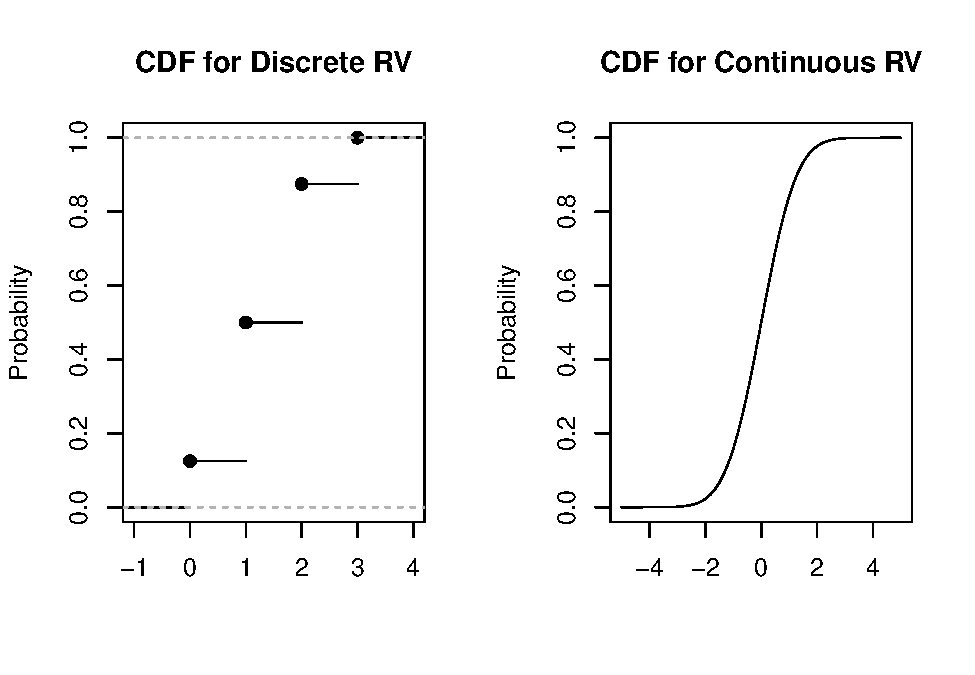
\includegraphics{bookdown-demo_files/figure-latex/4-compare-1.pdf}
\caption{\label{fig:4-compare}CDF for Discrete RV vs CDF for Continuous RV}
\end{figure}

As mentioned in the previous module, the CDF for a discrete random variable is what is called a step function, as it jumps at each value of the support. On the other hand, the CDF for a continuous random variable increases smoothly as its sample space is infinite.

The height of the CDF informs us the percentile associated with the value of the random variable. Looking at the CDF for the continuous random variable in Figure \ref{fig:4-compare}, the height is 0.5 when the random variable is 0, so a value of 0 corresponds to the 50th percentile of this distribution.

The technical definition of a continuous random variable is: A random variable has a continuous distribution if its CDF is differentiable.

A discrete random variable fails in this definition since its derivative is undefined at the jumps.

\subsection{Valid CDFs}\label{valid-cdfs-1}

The criteria for a valid CDF is the same, it does not matter if the random variable is discrete or continuous:

\begin{itemize}
\tightlist
\item
  non decreasing. This means that as \(x\) gets larger, the CDF either stays the same or increases. Visually, a graph of the CDF never decreases as \(x\) increases.
\item
  approach 1 as \(x\) approaches infinity and approach 0 as \(x\) approaches negative infinity. Visually, a graph of the CDF should be equal to or close to 1 for large values of x, and it should be equal to or close to 0 for small values of x.
\end{itemize}

\emph{Thought question}: Look at the CDFs for our example in Figure \ref{fig:4-compare}, and see how they satisfy the criteria listed above for a valid CDF.

\section{Probability Density Functions (PDFs)}\label{probability-density-functions-pdfs}

The \textbf{probability density function (PDF)} of a continuous random variable is analogous to the PMF of a discrete random variable.

The definition of the PDF for continuous random variables is the following: for a continuous random variable \(X\) with CDF \(F_X(x)\), the PDF of \(X\), \(f_X(x)\), is the derivative of its CDF, in other words, \(f_X(x) = F_X^{\prime}(x)\). The support of \(X\) is the set of \(x\) where \(f_X(x) >0\).

The relationship between the PDF and CDF of a continuous random variable \(X\) can be expressed as

\begin{equation} 
F_X(x) = P(X \leq x) = \int_{-\infty}^{x} f_X(x) dx.
\label{eq:4-PDFCDF}
\end{equation}

We take a look at an example below. Suppose we have a continuous random variable \(X\) with its CDF and PDF displayed below, and we want to find \(P(X \leq 1)\):

\begin{figure}
\centering
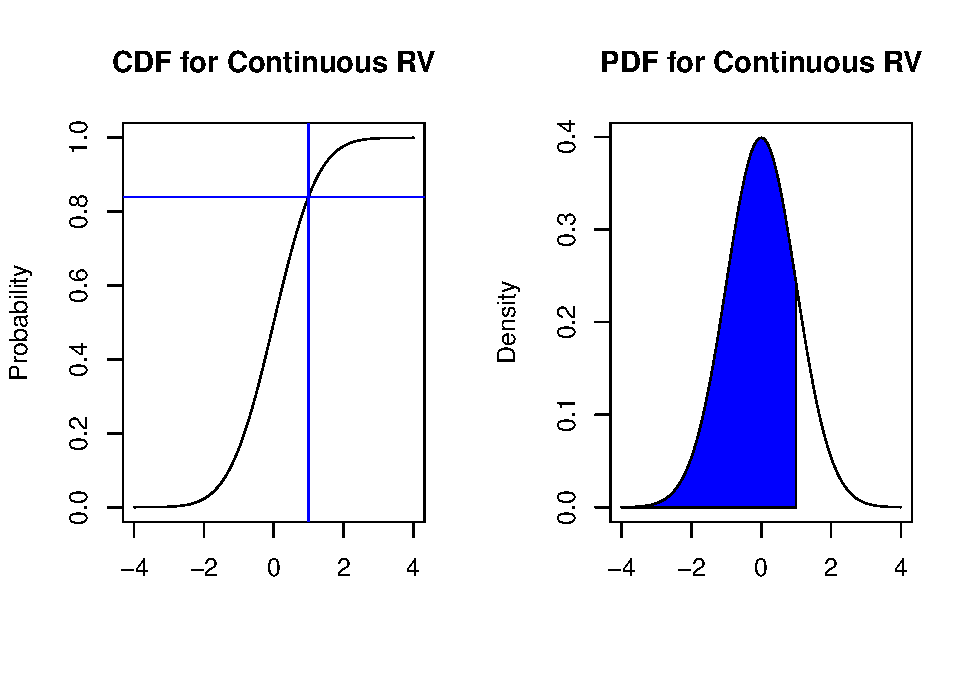
\includegraphics{bookdown-demo_files/figure-latex/4-prob-1.pdf}
\caption{\label{fig:4-prob}Probabilities from CDF and PDF}
\end{figure}

We can find \(P(X \leq 1)\) in two different ways:

\begin{itemize}
\tightlist
\item
  from the CDF, find the value of 1 on the horizontal axis, and read off the corresponding value on the vertical axis (blue lines). This tells us that \(P(X \leq 1) = 0.84\).
\item
  from the PDF, find the area under the PDF where \(X \leq 1\). This area corresponds to the shaded region in blue, and will be equal to 0.84 if we performed the integration per equation \eqref{eq:4-PDFCDF}.
\end{itemize}

Compare equation \eqref{eq:4-PDFCDF} with equation \eqref{eq:3-CDF} and note the similarities and differences in the CDFs for continuous and discrete random variables. For discrete CDFs, we sum the PMF over all values less than or equal to \(x\), whereas for continuous CDFs, we integrate, or accumulate the area, under the PDF over all values less than or equal to \(x\). Some people view the integral as a continuous version of a summation.

From equation \eqref{eq:4-PDFCDF}, we can generalize a way to find the probability \(P(a<X<b)\) for a continuous random variable \(X\):

\begin{equation} 
P(a<X<b) = F_X(b) - F_X(a) = \int_{a}^{b} f_X(x) dx.
\label{eq:4-integrate}
\end{equation}

In other words, to find the probability for a range of values for \(X\), we just find the area under its PDF for that range of values. Going back to our example, if we want to find \(P(0<X<1)\), we will find the area under its PDF for \(0<X<1\), like in Figure \ref{fig:4-prob2} below:

\begin{figure}
\centering
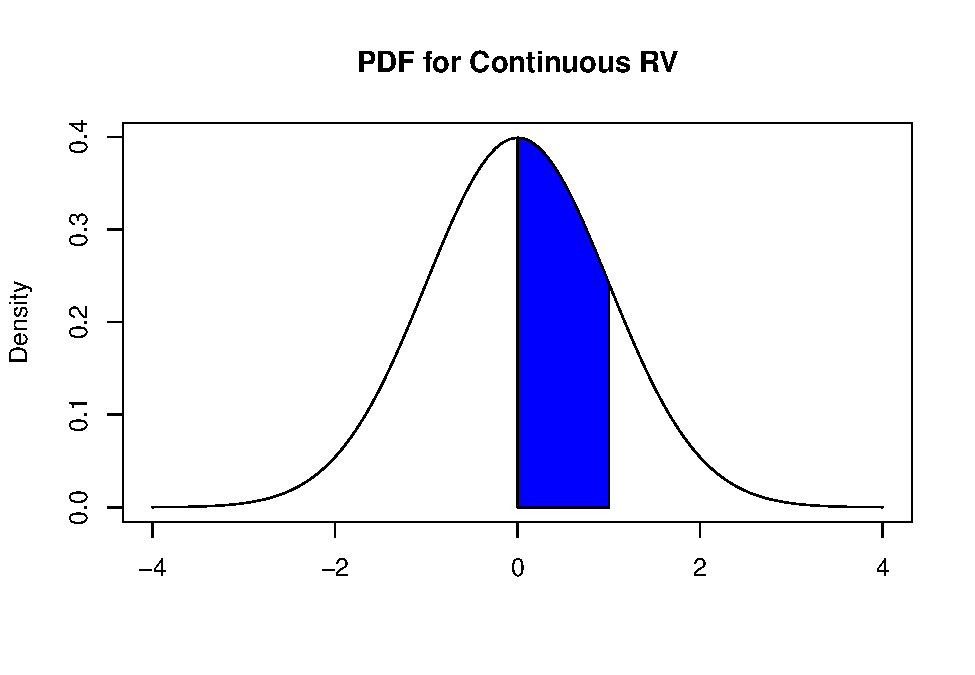
\includegraphics{bookdown-demo_files/figure-latex/4-prob2-1.pdf}
\caption{\label{fig:4-prob2}Probabilities from PDF}
\end{figure}

As mentioned, the PDF of a continuous random variable is analogous, but not exactly the same as, to the PMF of a discrete random variable. One common misconception is that the PDF tells us a probability, for example, that the value of \(f_X(2) = P(X=2)\), if \(X\) is continuous. This is only correct if \(X\) is discrete. In fact, if we look at equation \eqref{eq:4-integrate} a little more closely, \(P(X=c) = 0\) if \(X\) is continuous and \(c\) is a constant, since the area under its PDF will be 0.

\subsection{Valid PDFs}\label{valid-pdfs}

The PDF of a continuous random variable must satisfy the following criteria:

\begin{itemize}
\tightlist
\item
  Non negative: \(f_X(x) \geq 0\),
\item
  Integrates to 1: \(\int_{-\infty}^{\infty}f_X(x) dx = 1\).
\end{itemize}

\subsection{PDFs and Density Plots}\label{pdfs-and-density-plots}

Recall in Section \ref{pmfhist}, we learned that for discrete random variables, the PMF and histogram are related. The PMF represents the long-run proportion, while the histogram represents the relative frequency based on our data. As the sample size gets larger, the PMF should match the histogram.

Similarly for continuous random variables, the PDF and the density plot are related. The PDF is associated with the distribution of a known random variable, while the density plot is estimated from our data, and if our data follows a known random variable, the PDF should match the density plot as the sample size gets larger.

We will go over some of the details on how density plots are created at the end of this module, in Section \ref{KDE}, as we still need to cover a few concepts.

\section{Summaries of a Distribution}\label{summaries-of-a-distribution}

Next, we will talk about some common summaries associated with a distribution. These involve measures of centrality and variance, which we have covered before. We will also talk about a couple of other measures: skewness and kurtosis.

\subsection{Expectations}\label{expectations-1}

The \textbf{expected value} of a continuous random variable \(X\) is

\begin{equation} 
E(X) = \int_{-\infty}^{\infty} x f_X(x) dx.
\label{eq:4-EX}
\end{equation}

Another common notation for \(E(X)\) is \(\mu\), or sometimes \(\mu_X\) show that we are writing the mean of the random variable \(X\).

If we compare equation \eqref{eq:4-EX} with equation \eqref{eq:3-EX}, notice that we use an integral instead of a summation now that we are working with continuous random variables.

The interpretation of expected values is still the same: the expectation of a random variable can be interpreted as the long-run mean of the random variable, i.e.~if we were able to repeat the experiment an infinite number of times, the expectation of the random variable will be the average result among all the experiments. It is still a measure of centrality of the random variable.

The \textbf{linearity of expectations} still hold in the same way, per equation \eqref{eq:3-linEX}. It does not matter if the random variable is discrete or continuous.

The \textbf{Law of the Unconscious Statistician (LOTUS)} also still applies. For a continuous random variable \(X\), it is (unsurprisingly):

\begin{equation} 
E(g(X)) = \int_{-\infty}^{\infty} g(x) f_X(x) dx.
\label{eq:4-lotus}
\end{equation}

Notice again when we compare equation \eqref{eq:4-lotus} with its discrete counterpart in equation \eqref{eq:3-lotus}: we have just replaced the summation with an integral.

\emph{Thought question}: Can you guess how to write the equation for the variance of a continuous random variable? Hint: the variance for a discrete random variable is given in equation \eqref{eq:3-var2}.

\subsubsection{Median}\label{median-1}

The value \(m\) is the \textbf{median} of a random variable \(X\) if \(P(X \leq c) \geq \frac{1}{2}\) and \(P(X \geq c) \geq \frac{1}{2}\).

Intuitively, the median is the value \(m\) which splits the area under the PDF into half (or as close to half as possible if the random variable is discrete). Half the area will be to the left of \(m\), the other half of the area will be to the right of \(m\).

\subsubsection{Mode}\label{mode-1}

For a continuous random variable \(X\), the \textbf{mode} is the value \(c\) that maximizes the PDF: \(f_X(c) \geq f_X(x)\) for all \(x\).

For a discrete random variable \(X\), the mode is the value \(c\) that maximizes the PMF: \(P(X=c) \geq P(X=x)\) for all \(x\). Intuitively, the mode is the most commonly occurring value of a discrete random variable

\subsubsection{Loss Functions}\label{lossfunc}

A goal of statistical modeling is to use a model to make predictions. We want to be able to quantify the quality of our prediction, or the prediction error. Suppose we have an experiment that can be described by a random variable \(X\), and we want to predict the value of the next experiment. The mean and median are natural guesses for the value of the next experiment.

It turns out there a several ways to quantify our prediction error. These are usually called \textbf{loss functions}. Suppose our predicted value is denoted by \(x_{pred}\). A couple of common loss functions are:

\begin{itemize}
\tightlist
\item
  \textbf{Mean squared error (MSE)}: \(E(X-x_{pred})^2\),
\item
  \textbf{Mean absolute error (MAE)}: \(E|X-x_{pred}|\).
\end{itemize}

It turns out that the expected value \(E(X)\) minimizes the MSE, and the median minimizes the MAE. So depending on what loss function suits our analysis, we could use either the mean or median for our predictions. We will cover these ideas in more detail in a later module (and indeed in later courses in this program).

\subsection{Variance}\label{variance-1}

The \textbf{variance} of a continuous random variable \(X\) is

\begin{equation} 
Var(X) = \int_{-\infty}^{\infty} (x-\mu)^2 f_X(x) dx.
\label{eq:4-var}
\end{equation}

The properties of variance is still the same as in Section \ref{var-prop}. It does not matter if the random variable is discrete or continuous. A common notation used for variance is \(\sigma^2\), or sometimes \(\sigma_X^2\) to show it is the variance of the random variable \(X\).

\subsection{Moments}\label{moments}

Before talking about other measures that are used to describe continuous distributions, we will cover some terminology that is used for these measures. Suppose we have a random variable \(X\).

\begin{itemize}
\tightlist
\item
  The \textbf{\(k\)th moment} of \(X\) is \(E(X^k)\). So the expected value, or the mean, is sometimes called the first moment.
\item
  The \textbf{\(k\)th central moment} of \(X\) is \(E((X-\mu)^k)\). So the variance is sometimes called the second central moment.
\item
  The \textbf{\(k\) standardized moment} of \(X\) is \(E(\frac{(X-\mu)^k}{\sigma})\).
\end{itemize}

\subsection{Skewness}\label{skewness}

One measure that is used to describe the shape of a distribution is skewness, which is a measure of symmetry (or measure of skewness). The \textbf{skew} of a random variable \(X\) is the third standardized moment:

\begin{equation} 
Skew(X) = E \left(\frac{(X-\mu)^3}{\sigma} \right)
\label{eq:4-skew}
\end{equation}

A random variable \(X\) has a \textbf{symmetric distribution about its mean} if \(X - \mu\) has the same distribution as \(\mu - X\). Fairly often, people will just say that \(X\) is symmetric; it is almost always assumed that the symmetry is about its mean.

Intuitively, symmetry means that the PDF of \(X\) to the left of its mean is the mirror image of the PDF of \(X\) to the right of its mean. We look at a couple of examples below in Figure \ref{fig:4-symm}:

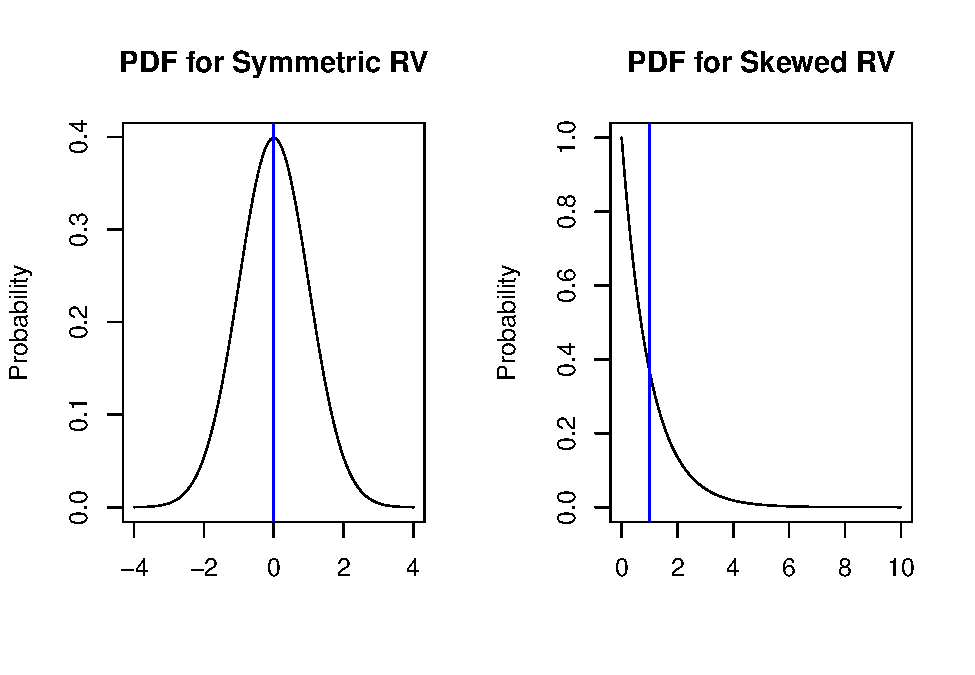
\includegraphics{bookdown-demo_files/figure-latex/4-symm-1.pdf}
The blue vertical lines indicate the mean of these distributions. Notice the mirror image in the first plot, but not in the second plot.

If a distribution is not symmetric, we can say its distribution is asymmetric, or is skewed. The values of \(Skew(X)\) that are associated with different shapes are:

\begin{itemize}
\tightlist
\item
  \(Skew(X) = 0\): \(X\) is symmetric.
\item
  \(Skew(X) > 0\): \(X\) is right (or positively) skewed.
\item
  \(Skew(X) < 0\): \(X\) is left (or negatively) skewed.
\end{itemize}

\subsection{Kurtosis}\label{kurtosis}

One more measure deals with the \textbf{tail} behavior of a distribution. Visually, the tails of a PDF are associated with probabilities of extreme values for a random variable. A distribution that is heavy tailed means that extreme values (on both ends) are more likely to occur. Tail behavior is an important consideration in risk management in finance: e.g.~a heavy left tail in the PDF could mean a financial crisis. Figure \ref{fig:4-kurt} shows an example of a heavy tailed distribution (in blue), compared to a Gaussian distribution (in black). We will talk more about the Gaussian distribution in the next subsection.

\begin{figure}
\centering
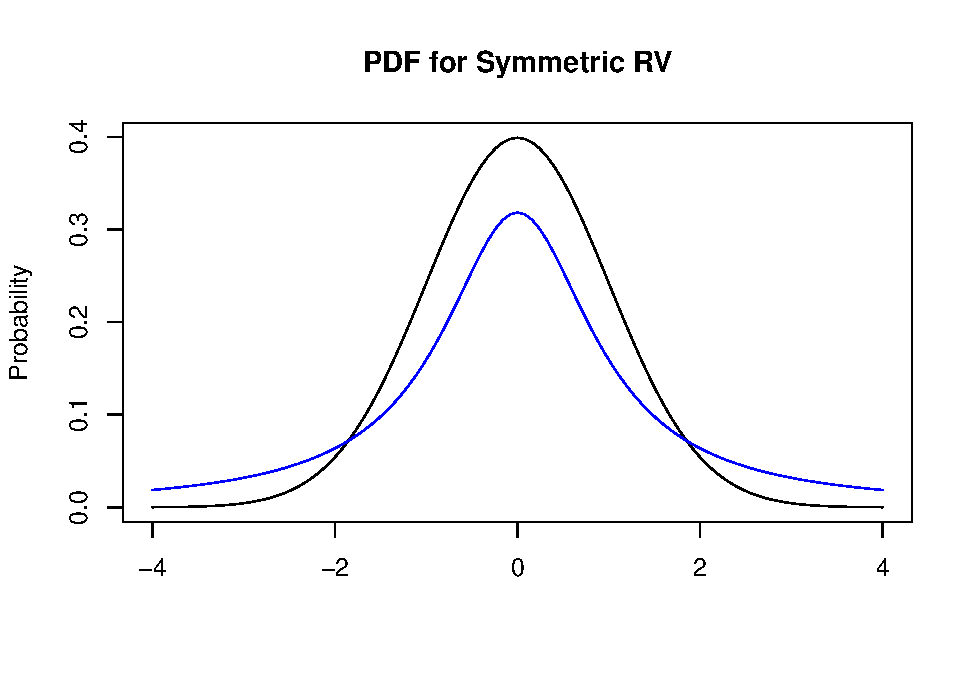
\includegraphics{bookdown-demo_files/figure-latex/4-kurt-1.pdf}
\caption{\label{fig:4-kurt}PDF for Heavy Tailed Distribution}
\end{figure}

A common measure of tail behavior is the \textbf{Kurtosis}. The kurtosis of a random variable \(X\) is the shifted fourth standardized moment:

\begin{equation} 
Kurt(X) = E \left(\frac{(X-\mu)^4}{\sigma} \right) - 3.
\label{eq:4-kurt}
\end{equation}

The reason for subtracting (or shifting by) 3 is so that the Gaussian distribution (a commonly used distribution for continuous random variables) has a kurtosis of 0. Note: Some authors call equation \eqref{eq:4-kurt} the \textbf{excess kurtosis} and the kurtosis does not subtract the 3.

The values of \(Kurt(X)\) that are associated with tail behaviors are:

\begin{itemize}
\tightlist
\item
  \(Kurt(X) = 0\): \(X\) is similar tails to Gaussian distribution.
\item
  \(Kurt(X) > 0\): \(X\) has heavier tails compared to Gaussian distribution (extreme values more likely).
\item
  \(Kurt(X) < 0\): \(X\) has smaller tails compared to Gaussian distribution (extreme values less likely).
\end{itemize}

\section{Common Continuous Random Variables}\label{common-continuous-random-variables}

Next, we will introduce some commonly used distributions that may be used for continuous random variables. A number of common statistical models (for example, linear regression) are based on these distributions.

\subsection{Uniform}\label{uniform}

A random variable that follows a uniform distribution on the interval \((a,b)\) is a completely random number between \(a\) and \(b\). Notionally, an upper case \(U\) is usually used to denote a uniform random variable. \(U\) is said to have a \textbf{uniform distribution} on the interval \((a,b)\), denoted as \(U \sim(a,b)\), if its PDF is

\begin{equation} 
f_X(x) = \begin{cases} 
  \frac{1}{b-a} & \text{if } a<x<b \\
  0 & \text{otherwise }. 
\end{cases}
\label{eq:4-U}
\end{equation}

Note that the parameters \(a,b\) also help define the support of a uniform distribution. Figure \ref{fig:4-U} below displays a plot of the PDF of a \(U(a,b)\):

\begin{figure}
\centering
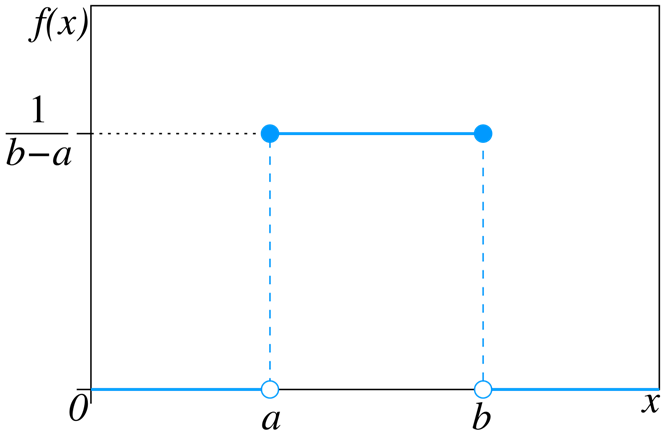
\includegraphics{images/04-U.png}
\caption{\label{fig:4-U}PDF of U(a,b). Picture from \url{https://en.wikipedia.org/wiki/Continuous_uniform_distribution}}
\end{figure}

\emph{Thought question}: Can you verify that this is a valid PDF?

Figure \ref{fig:4-Ucdf} below displays a plot of the CDF of a \(U(a,b)\):

\begin{figure}
\centering
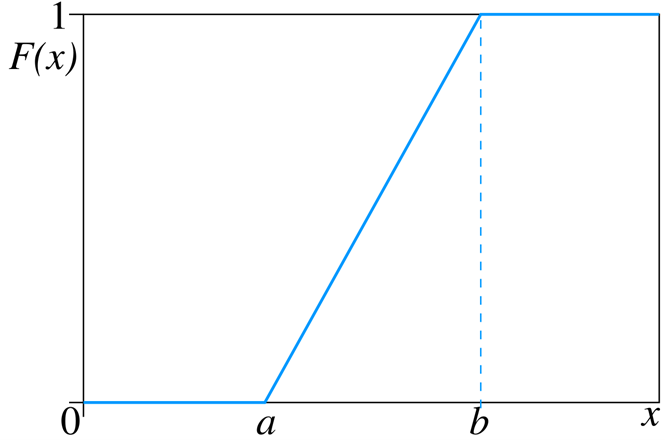
\includegraphics{images/04-Ucdf.png}
\caption{\label{fig:4-Ucdf}CDF of U(a,b). Picture from \url{https://en.wikipedia.org/wiki/Continuous_uniform_distribution}}
\end{figure}

Some properties of the uniform distribution:

\begin{itemize}
\tightlist
\item
  Its mean is \(E(U) = \frac{a+b}{2}\).
\item
  Its variance is \(Var(U) = \frac{(b-a)^2}{12}\).
\item
  Its skewness is 0, so it is symmetric.
\item
  Its kurtosis is -\(\frac{6}{5}\), so its tails are not as heavy compared to a Gaussian distribution.
\end{itemize}

\emph{Thought question}: Can you see why a uniform distribution is symmetric? Can you see why its tails are not heavy?

If the support of a uniform distribution is between 0 and 1, we have a \textbf{standard uniform distribution}. We will talk about the importance of the standard uniform distribution in the next subsection.

\subsubsection{Universality of Uniform}\label{universality-of-uniform}

It turns out that we can construct a random variable with any continuous distribution based on a standard uniform distribution. This fact is used to simulate random numbers from continuous distributions. This fact is called the \textbf{Universality of the Uniform}: Let \(F_X(x)\) denote the CDF of a continuous random variable \(X\), then:

\begin{enumerate}
\def\labelenumi{\arabic{enumi}.}
\tightlist
\item
  Let \(U \sim U(0,1)\) and \(X = F^{-1}(U)\). Then \(X\) is a random variable with CDF \(F_X(x)\).
\item
  \(F_X(X) \sim U(0,1)\).
\end{enumerate}

To give some insight into what this means, we look at an example. Another continuous distribution is called the standard logistic distribution, which we will denote with \(X\). Its CDF is

\[
F_X(x) = \frac{e^x}{1+e^x}.
\]
Let \(U \sim U(0,1)\). The first part of the universality of the uniform informs us that the inverse of the CDF for the standard logistic is \(F_X^{-1}(U) \sim X\), so we invert \(F_X(x)\) to get its inverse \(F_X^{-1}(x)\). This is done by setting the CDF of \(X\) to be equal to \(u\), i.e.~let \(u = \frac{e^x}{1+e^x}\), and solving for \(x\):

\[
\begin{split}
u + u e^x &= e^x\\
\implies u &= e^x (1-u) \\
\implies e^x &= \frac{u}{1-u} \\
\implies x &= \log (\frac{u}{1-u}).
\end{split}
\]

Therefore \(F^{-1}(u) = \log (\frac{u}{1-u})\) and \(F^{-1}(U) = \log (\frac{U}{1-U})\). Therefore \(\log (\frac{U}{1-U})\) follows a standard logistic distribution.

Let us use simulations to show what is going on. First, we simulate 10,000 reps from a standard uniform distribution, then invert these values using \(\log (\frac{u}{1-u})\), and create the density plot of \(\log (\frac{u}{1-u})\). These steps are shown in Figure \ref{fig:4-universe} below:

\begin{Shaded}
\begin{Highlighting}[]
\FunctionTok{set.seed}\NormalTok{(}\DecValTok{4}\NormalTok{)}

\NormalTok{reps}\OtherTok{\textless{}{-}}\DecValTok{10000} \DocumentationTok{\#\#number of reps}
\NormalTok{u}\OtherTok{\textless{}{-}}\FunctionTok{runif}\NormalTok{(reps) }\DocumentationTok{\#\#simulate standard uniform}
\NormalTok{invert}\OtherTok{\textless{}{-}} \FunctionTok{log}\NormalTok{(u}\SpecialCharTok{/}\NormalTok{(}\DecValTok{1}\SpecialCharTok{{-}}\NormalTok{u)) }\DocumentationTok{\#\#invert based on F inverse. These should now follow standard logistic}

\FunctionTok{par}\NormalTok{(}\AttributeTok{mfrow=}\FunctionTok{c}\NormalTok{(}\DecValTok{1}\NormalTok{,}\DecValTok{3}\NormalTok{))}
\FunctionTok{plot}\NormalTok{(}\FunctionTok{density}\NormalTok{(u), }\AttributeTok{main=}\StringTok{"Density Plot from 10,000 U\textquotesingle{}s"}\NormalTok{)}
\FunctionTok{plot}\NormalTok{(}\FunctionTok{density}\NormalTok{(invert), }\AttributeTok{main=}\StringTok{"Density Plot after Inverting"}\NormalTok{, }\AttributeTok{xlim=}\FunctionTok{c}\NormalTok{(}\SpecialCharTok{{-}}\DecValTok{6}\NormalTok{,}\DecValTok{6}\NormalTok{))}
\FunctionTok{curve}\NormalTok{(dlogis, }\AttributeTok{from =} \SpecialCharTok{{-}}\DecValTok{7}\NormalTok{, }\AttributeTok{to =} \DecValTok{7}\NormalTok{, }\AttributeTok{main =} \StringTok{"PDF for Logistic"}\NormalTok{, }\AttributeTok{ylab=}\StringTok{"Density"}\NormalTok{, }\AttributeTok{xlab=}\StringTok{""}\NormalTok{)}
\end{Highlighting}
\end{Shaded}

\begin{figure}
\centering
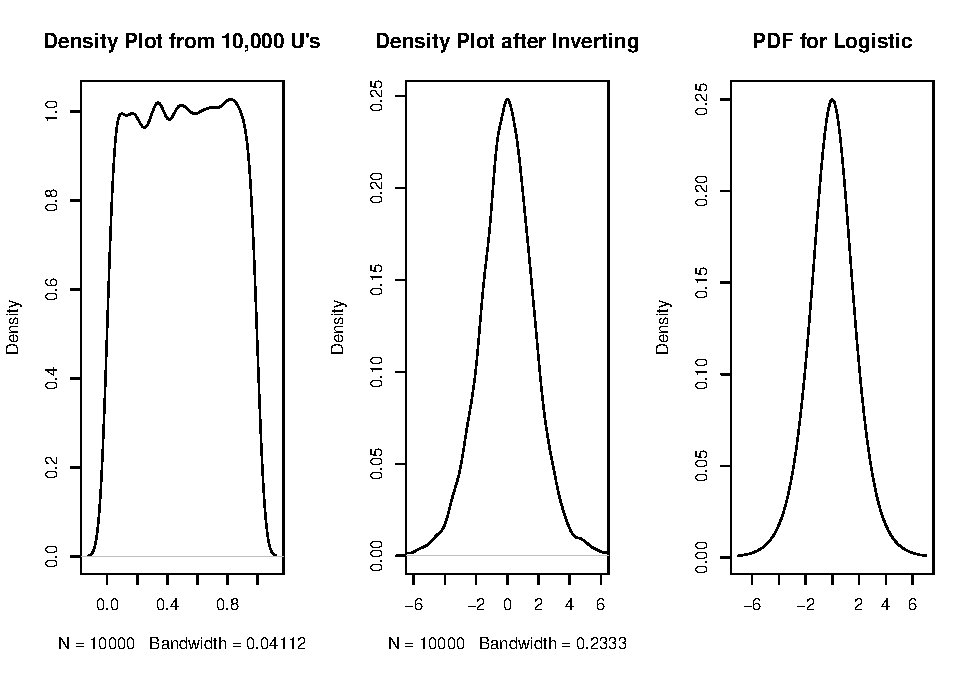
\includegraphics{bookdown-demo_files/figure-latex/4-universe-1.pdf}
\caption{\label{fig:4-universe}Uniform to Logistic}
\end{figure}

From Figure \ref{fig:4-universe}:

\begin{itemize}
\tightlist
\item
  The first plot shows the density plot from our 10,000 reps from a standard normal. This is close to the PDF of a standard uniform.
\item
  The second plot shows the density plot after inverting our 10,000 reps from a standard normal, i.e.~\(F^{-1}(u) = \log (\frac{u}{1-u})\).
\item
  The third plot shows the PDF of a standard logistic. Notice how similar this looks to the second plot.
\end{itemize}

So we see that \(\log (\frac{U}{1-U})\) follows a standard logistic distribution.

View the video below for a more detailed explanation of this example:

The second part of the universality of the uniform informs us that if \(X\) follows a standard logistic distribution, then \(F(X) = \frac{e^X}{1 + e^X} \sim U(0,1)\).

So, we can see the purpose of the universality of the uniform:

\begin{itemize}
\tightlist
\item
  For part 1, we can simulate reps from any distribution, as long as we know its CDF. The software you use may not be able to simulate reps from a particular distribution, but you can write code to simulate reps from this distribution based on the standard uniform.
\item
  For part 2, we can convert a random variable with an unknown distribution to one that is known: the standard uniform.
\end{itemize}

\subsection{Normal}\label{normdist}

Another widely used distribution for continuous random variables is the \textbf{normal}, or \textbf{Gaussian} distribution. This is a distribution that is symmetric and bell-shaped. This is probably the most important distribution in statistics and data science due to the Central Limit Theorem. We will define this theorem in a later module, but loosely speaking, it says that if we take the average of a bunch of random variables, the average will approximate a normal distribution, even if the random variables are individually not normal.

A lot of questions that we wish to answer are based on averages. For example

\begin{itemize}
\tightlist
\item
  Does the implementation of certain technologies in a class improve test scores for students, on average?
\item
  Are male Gentoo penguins heavier than their female counterparts, on average?
\item
  Does replacing traffic lights with a roundabout reduce the number of traffic accidents, on average?
\end{itemize}

What the central limit theorem implies is that even if test scores, weights of Gentoo penguins, and number of traffic accidents do not follow a normal distribution, their average values will approximate a normal distribution.

\subsubsection{Standard Normal}\label{standard-normal}

First, we will talk about the \textbf{standard normal distribution}, as other normal distributions can be viewed as variations of the standard normal. A standard normal distribution has mean 0 and variance 1. It is usually denoted by \(Z\). We can also write \(Z \sim N(0,1)\) to say that \(Z\) is normally distributed with mean 0 and variance 1. The PDF of a standard normal distribution is:

\begin{equation} 
\phi(z) = \frac{1}{\sqrt{2 \pi}} e^{-z^2/2}.
\label{eq:4-Z}
\end{equation}

Notice the constant \(\frac{1}{\sqrt{2 \pi}}\) in equation \eqref{eq:4-Z}. Its presence is needed to make the PDF valid, since the PDF must integrate to 1. Such constants are called \textbf{normalizing constants}.

Figure \ref{fig:4-Z} below displays its PDF:

\begin{Shaded}
\begin{Highlighting}[]
\FunctionTok{curve}\NormalTok{(dnorm, }\AttributeTok{from =} \SpecialCharTok{{-}}\DecValTok{4}\NormalTok{, }\AttributeTok{to =} \DecValTok{4}\NormalTok{, }\AttributeTok{main =} \StringTok{"PDF for Z"}\NormalTok{, }\AttributeTok{ylab=}\StringTok{"Density"}\NormalTok{, }\AttributeTok{xlab=}\StringTok{""}\NormalTok{)}
\end{Highlighting}
\end{Shaded}

\begin{figure}
\centering
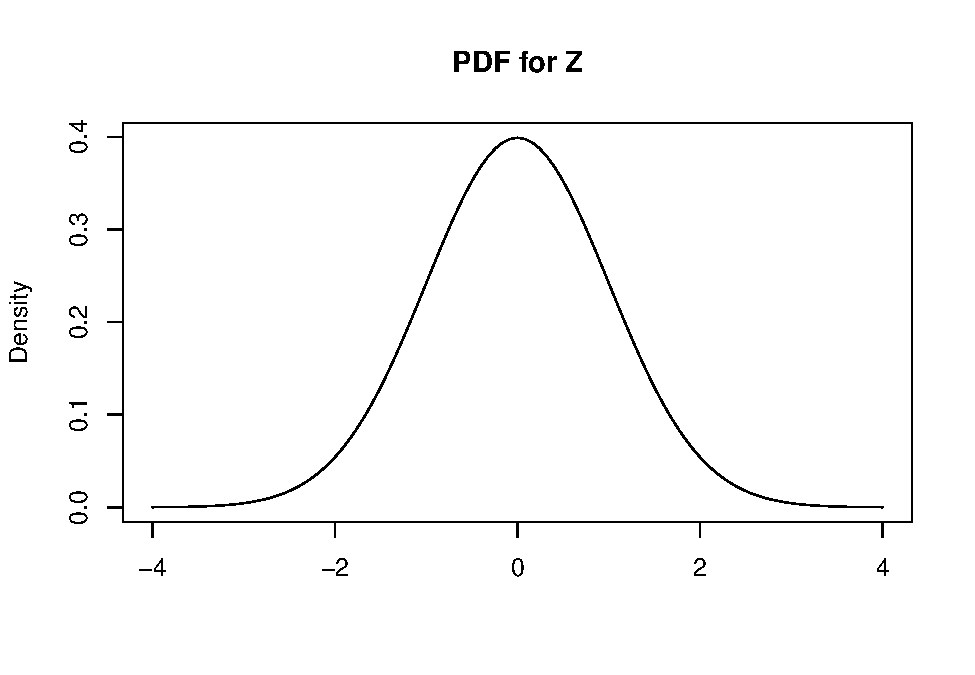
\includegraphics{bookdown-demo_files/figure-latex/4-Z-1.pdf}
\caption{\label{fig:4-Z}PDF of Standard Normal}
\end{figure}

From Figure \ref{fig:4-Z}, we can see the following properties of a standard normal distribution (these will apply for any normal distribution):

\begin{itemize}
\tightlist
\item
  Its PDF is symmetric about its mean. In Figure \ref{fig:4-Z}, the PDF is symmetric about 0, i.e.~\(\phi(-z) = \phi(z)\).
\item
  This implies that the tail areas are also symmetric. For example, \(P(Z \leq -2) = P(Z \geq 2)\).
\item
  Its skew is 0, since it is symmetric.
\end{itemize}

There is actually no closed-formed equation for the CDF of a standard normal (or any normal distribution). We write \(\Phi(z) = P(Z \leq z) = \int_{\infty}^z \phi(z) dz\) to express the CDF of a standard normal.

Notice that we have special letters \(Z, \phi, \Phi\) to denote the standard normal distribution. This is an indication of how often it is used to warrant its own notation.

\subsubsection{From Standard Normal to Other Normals}\label{norm}

If \(Z \sim N(0,1)\), then \(X = \mu + \sigma Z \sim N(\mu, \sigma^2)\). In other words, if \(Z\) is standard normal, then \(X = \mu + \sigma Z\) follows a normal distribution with mean \(\mu\) and variance \(\sigma^2\). The parameters of a normal distribution are the mean \(\mu\) and variance \(\sigma^2\).

Note that some authors say the parameters are the mean \(\mu\) and standard deviation \(\sigma\) instead, so be careful when reading notation associated with normal distributions from various sources. For example, \(N(0,2)\) in our class and our book means normal distribution with mean 0 and variance 2, but for some other authors, \(N(0,2)\) means normal distribution with mean 0 and standard deviation 2. Indeed, the functions in R use this alternate parameterization, so you need to be careful.

\emph{Thought question}: Can you use the linearity of expectations to explain why \(X\) has mean \(\mu\)? Can you use properties of variance from Section \ref{var-prop} to explain why \(X\) has variance \(\sigma^2\)?

Notice how we started from a standard normal \(Z\), and transformed \(Z\) by multiplying it by \(\sigma\) and then adding \(\mu\) to get any normal distribution. This transformation is called a \textbf{location-scale} transformation, or shifting and scaling. The scale changes since we multiply by a constant \(\sigma\); the location is transformed since its mean changes from 0 to \(\mu\).

We can also reverse this transformation and state the following: If \(X \sim N(\mu, \sigma^2)\), then \(Z = \frac{X-\mu}{\sigma} \sim N(0,1)\). If we start with \(X \sim N(\mu, \sigma^2)\), then we can transform \(X\) by subtracting \mu, and then dividing by \(\sigma\), to obtain \(Z\). This particular transformation is called \textbf{standardization}:

\begin{equation} 
Z = \frac{X-\mu}{\sigma}.
\label{eq:4-standardize}
\end{equation}

The PDF of any normal distribution \(X \sim N(\mu, \sigma^2)\) is

\begin{equation} 
f_X(x) = \frac{1}{\sigma \sqrt{2 \pi}} \exp \left(-\frac{(x - \mu)^2}{2 \sigma^2} \right).
\label{eq:4-pdfNormal}
\end{equation}

\emph{Thought question}: Compare equations \eqref{eq:4-pdfNormal} and \eqref{eq:4-Z}. Can you see how equation \eqref{eq:4-Z} can be derived from equation \eqref{eq:4-pdfNormal}?

\subsubsection{68-95-99.7\% Rule}\label{rulenorm}

The following property holds for any normal distribution, and is often called the \textbf{68-99-99.7\%} rule. For any normal distribution \(X \sim N(\mu, \sigma^2)\):

\begin{itemize}
\tightlist
\item
  \(P(\mu - \sigma < X < \mu + \sigma) \approx 0.68\),
\item
  \(P(\mu - 2\sigma < X < \mu + 2\sigma) \approx 0.95\),
\item
  \(P(\mu - 3\sigma < X < \mu + 3\sigma) \approx 0.997\).
\end{itemize}

What these mean is that for any normal distribution:

\begin{itemize}
\tightlist
\item
  About 68\% of observed values will fall within 1 standard deviation of the mean,
\item
  About 95\% of observed values will fall within 2 standard deviations of the mean, and
\item
  About 99.7\% of observed values will fall within 3 standard deviations of the mean.
\end{itemize}

The last statement is the basis for the term \href{https://en.wikipedia.org/wiki/Six_Sigma}{six sigma} used in manufacturing, since virtually all data points should fall within a range that is six sigma wide (assuming they follow a normal distribution). Visually, this rule is shown in Figure \ref{fig:4-rule} when applied to the standard normal:

\begin{figure}
\centering
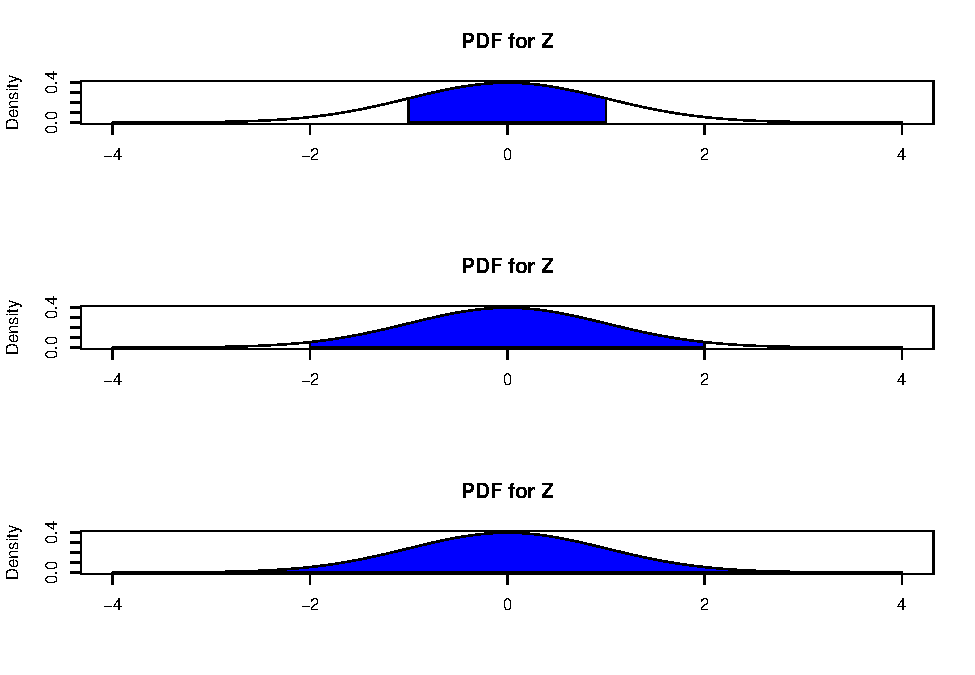
\includegraphics{bookdown-demo_files/figure-latex/4-rule-1.pdf}
\caption{\label{fig:4-rule}68-95-99.7 Rule}
\end{figure}

We will work out the first statement, that about 68\% of the observed values will fall within 1 standard deviation of the mean for any normal distribution. We will use R to help us verify this rule for a standard normal:

\begin{Shaded}
\begin{Highlighting}[]
\NormalTok{upper1}\OtherTok{\textless{}{-}}\FunctionTok{pnorm}\NormalTok{(}\DecValTok{1}\NormalTok{) }\DocumentationTok{\#\# what is percentile associated with Z=1 (i.e. 1 standard deviation above mean)}
\NormalTok{lower1}\OtherTok{\textless{}{-}}\FunctionTok{pnorm}\NormalTok{(}\SpecialCharTok{{-}}\DecValTok{1}\NormalTok{) }\DocumentationTok{\#\# what is percentile associated with Z={-}1 (i.e. 1 standard deviation below mean)}
\NormalTok{upper1}\SpecialCharTok{{-}}\NormalTok{lower1 }\DocumentationTok{\#\# find proportion in between 1 SD above and below mean.}
\end{Highlighting}
\end{Shaded}

\begin{verbatim}
## [1] 0.6826895
\end{verbatim}

\emph{Thought question}: how would you tweak this code to verify the other two statements associated with the 68-95-99.7\% rule?

\section{Using R}\label{usingR}

R has built in functions to compute the density, CDF, percentiles, as well as simulate data of common distributions. We will start with a random variable \(Y \sim N(1, 9)\) as an example.

\begin{enumerate}
\def\labelenumi{\arabic{enumi}.}
\tightlist
\item
  To find \(f_Y(2)\), use:
\end{enumerate}

\begin{Shaded}
\begin{Highlighting}[]
\FunctionTok{dnorm}\NormalTok{(}\DecValTok{2}\NormalTok{, }\DecValTok{1}\NormalTok{, }\DecValTok{3}\NormalTok{) }\DocumentationTok{\#\#supply the value of Y you want, then the parameters mu and sigma}
\end{Highlighting}
\end{Shaded}

\begin{verbatim}
## [1] 0.1257944
\end{verbatim}

The density \(f_Y(2)\) is 0.1257944. Note: In R, the normal distribution is parameterized by the mean and standard deviation, which is different from these set of notes and our book, which uses the mean and variance.

\begin{enumerate}
\def\labelenumi{\arabic{enumi}.}
\setcounter{enumi}{1}
\tightlist
\item
  To find \(P(Y \leq 2)\), use:
\end{enumerate}

\begin{Shaded}
\begin{Highlighting}[]
\FunctionTok{pnorm}\NormalTok{(}\DecValTok{2}\NormalTok{, }\DecValTok{1}\NormalTok{, }\DecValTok{3}\NormalTok{) }\DocumentationTok{\#\#supply the value of Y you want, then the parameters mu and sigma}
\end{Highlighting}
\end{Shaded}

\begin{verbatim}
## [1] 0.6305587
\end{verbatim}

The probability that \(Y\) is less than or equal to 2 is 0.6305587.

Alternatively, we can standardize this normal distribution, and use the standard normal. The standardization, per equation \eqref{eq:4-standardize}, gives us

\[
z = \frac{2-1}{3} = \frac{1}{3},
\]

so

\[
\begin{split}
P(Y \leq 2) &= P(\frac{Y-\mu}{\sigma} \leq \frac{2-1}{3}) \\
            &= P(Z \leq \frac{1}{3}) \\
            &= \Phi(\frac{1}{3})
\end{split}
\]

which can be found using

\begin{Shaded}
\begin{Highlighting}[]
\FunctionTok{pnorm}\NormalTok{(}\DecValTok{1}\SpecialCharTok{/}\DecValTok{3}\NormalTok{) }\DocumentationTok{\#\#don\textquotesingle{}t supply mu and sigma means you want to use standard normal}
\end{Highlighting}
\end{Shaded}

\begin{verbatim}
## [1] 0.6305587
\end{verbatim}

which gives the same answer as \texttt{pnorm(2,1,3)}.

View the video below for a more detailed explanation of this example:

\begin{enumerate}
\def\labelenumi{\arabic{enumi}.}
\setcounter{enumi}{2}
\tightlist
\item
  To find the value on the support that corresponds to the 90th percentile, use:
\end{enumerate}

\begin{Shaded}
\begin{Highlighting}[]
\FunctionTok{qnorm}\NormalTok{(}\FloatTok{0.9}\NormalTok{, }\DecValTok{1}\NormalTok{, }\DecValTok{3}\NormalTok{) }\DocumentationTok{\#\#supply the value of the percentile you need, then the parameters mu and sigma}
\end{Highlighting}
\end{Shaded}

\begin{verbatim}
## [1] 4.844655
\end{verbatim}

The 90th percentile of \(Y \sim N(1,9)\) is 4.844655.

If we want to use the standard normal, we could find its 90th percentile:

\begin{Shaded}
\begin{Highlighting}[]
\FunctionTok{qnorm}\NormalTok{(}\FloatTok{0.9}\NormalTok{)}
\end{Highlighting}
\end{Shaded}

\begin{verbatim}
## [1] 1.281552
\end{verbatim}

and then apply the location scale transformation

\begin{Shaded}
\begin{Highlighting}[]
\FunctionTok{qnorm}\NormalTok{(}\FloatTok{0.9}\NormalTok{)}\SpecialCharTok{*}\DecValTok{3} \SpecialCharTok{+} \DecValTok{1} \DocumentationTok{\#\#multiply by sigma, then add mu}
\end{Highlighting}
\end{Shaded}

\begin{verbatim}
## [1] 4.844655
\end{verbatim}

which is the same answer as \texttt{qnorm(0.9,1,3)}.

\begin{enumerate}
\def\labelenumi{\arabic{enumi}.}
\setcounter{enumi}{3}
\tightlist
\item
  To simulate 10 draws (replicates) of \(Y\), use:
\end{enumerate}

\begin{Shaded}
\begin{Highlighting}[]
\FunctionTok{set.seed}\NormalTok{(}\DecValTok{2}\NormalTok{) }\DocumentationTok{\#\#use set.seed() so we get the same random numbers each time the code is run}
\FunctionTok{rnorm}\NormalTok{(}\DecValTok{10}\NormalTok{, }\DecValTok{1}\NormalTok{, }\DecValTok{3}\NormalTok{) }\DocumentationTok{\#\#supply the number of simulated data you need, then the parameters mu and sigma}
\end{Highlighting}
\end{Shaded}

\begin{verbatim}
##  [1] -1.6907436  1.5545476  5.7635360 -2.3911270  0.7592447  1.3972609
##  [7]  3.1238642  0.2809059  6.9534218  0.5836390
\end{verbatim}

This outputs a vector of length 10. Each value represents the result of each rep. So the first value drawn from \(Y \sim N(1,9)\) -1.6907436, the second value drawn is 1.5545476 and so on.

Just like in Section \ref{Rdis}, notice these functions all ended with \texttt{norm}. We just added a different letter first, depending on whether we want the density (analogous to PDF), CDF, percentile, or random draw. The letters are \texttt{d}, \texttt{p}, \texttt{q}, and \texttt{r} respectively.

One thing to note: if we do not supply the mean and standard deviation, for example we type \texttt{rnorm(10)}, R will assume you want to use a standard normal distribution, so \texttt{rnorm(10)} will draw 10 random numbers from a standard normal.

\subsection{Density Plots and Kernel Density Estimation}\label{KDE}

We are now ready to talk about how density plots, like the ones in Figure \ref{fig:4-universe} are created. Recall the difference between density plots and PDFs:

\begin{itemize}
\tightlist
\item
  A plot of the PDF describes the distribution of a known random variable.
\item
  A density plot is based on our data, and is used to describe the distribution of our data. Our data may or may not follow a commonly known random variable. If it does, then a plot of the PDF and the density plot should match up as we gather more and more data.
\end{itemize}

Proportions are found in the same way, by finding the area under the PDF or density plot for the appropriate range on the support.

Suppose we have \(n\) observed values of an unknown random variable \(X\): \(x_1, x_2, \cdots, x_n\).The density \(f\) of \(X\) is unknown and we want to estimate it with our data. To estimate the density \(f\), we use the \textbf{kernel density estimator}:

\begin{equation} 
\hat{f}_h(x) = \frac{1}{nh} \sum_{i=1}^n K \left( \frac{x-x_i}{h}\right ),
\label{eq:4-KDE}
\end{equation}

where \(K\) is the \textbf{kernel} and \(h\) is a smoothing parameter, often called the \textbf{bandwidth}. Looking at equation \eqref{eq:4-KDE}, the KDE can be viewed as a weighted average of the relative likelihood of observing a particular value.

The kernel can be viewed as a weighting function, with the weights following the shape of a distribution that the user specifies (usually symmetric). Common kernel functions and their shapes are displayed in Figure \ref{fig:4-KDE}:

\begin{figure}
\centering
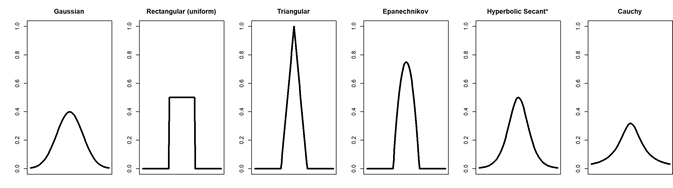
\includegraphics{images/04-KDE.png}
\caption{\label{fig:4-KDE}Common Kernals. Picture adapted from \url{https://tgstewart.cloud/compprob/kde.html}}
\end{figure}

The horizontal axis on the kernel can be viewed as the distance of the value of a data point from a specific value on the support, and the mid point on the horizontal axis represents a distance of 0.

\begin{itemize}
\tightlist
\item
  Looking at the normal kernel, nearest values receive the highest weight, and values further away receive less weight.
\item
  For the uniform kernel, values within a certain distance receive a weight, and values beyond a certain distance receive no weight.
\item
  The Epanechnikov (parabolic) kernel is a mix of both: values beyond a certain distance receive no weight, and values within a certain distance receive a weight that is roughly inversely proportional to the distance.
\end{itemize}

\(h\) is the smoothing parameter and is analogous to bin width in histograms. Larger values result in smoother looking density plots.

Let us go back to an old example. We will use the \texttt{loan50} dataset from the \texttt{openintro} package. The data originally consist of thousands of loans made through the Lending Club platform, but we will randomly select 50 of these loans. Let us study the interest rate the loans the 50 applicants received.

\begin{Shaded}
\begin{Highlighting}[]
\FunctionTok{library}\NormalTok{(openintro)}

\DocumentationTok{\#\#create object for data}
\NormalTok{Data}\OtherTok{\textless{}{-}}\NormalTok{loan50}

\DocumentationTok{\#\#create density plot using default}
\FunctionTok{plot}\NormalTok{(}\FunctionTok{density}\NormalTok{(Data}\SpecialCharTok{$}\NormalTok{interest\_rate), }\AttributeTok{main=}\StringTok{"Density Plot of Interest Rates"}\NormalTok{)}
\end{Highlighting}
\end{Shaded}

\begin{figure}
\centering
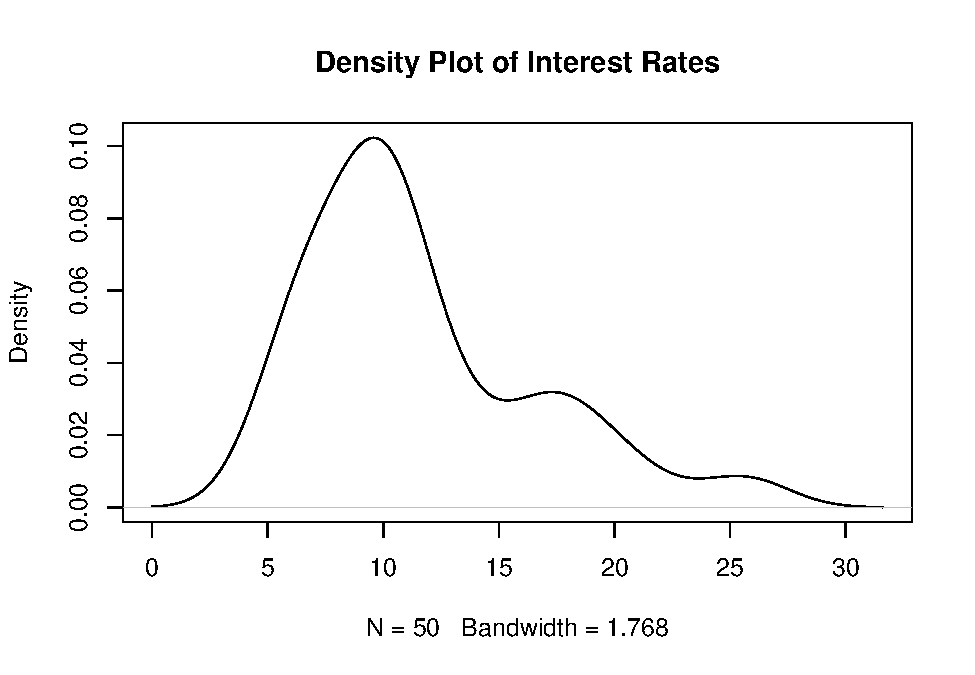
\includegraphics{bookdown-demo_files/figure-latex/4-R-1.pdf}
\caption{\label{fig:4-R}Density Plot for 50 Interest Rates}
\end{figure}

This uses KDE with the default settings: kernel is normal, and the bandwidth is based on \href{https://en.wikipedia.org/wiki/Kernel_density_estimation\#A_rule-of-thumb_bandwidth_estimator}{Silverman's rule of thumb}.

To change these, we add the \texttt{kernel} and \texttt{adjust} argument when using the \texttt{density()} function, for example, to use the Epanechnikov kernel with twice the default bandwidth:

\begin{Shaded}
\begin{Highlighting}[]
\DocumentationTok{\#\#create density plot using different settings}
\FunctionTok{plot}\NormalTok{(}\FunctionTok{density}\NormalTok{(Data}\SpecialCharTok{$}\NormalTok{interest\_rate, }\AttributeTok{kernel =} \StringTok{"epanechnikov"}\NormalTok{, }\AttributeTok{adjust =} \DecValTok{2}\NormalTok{), }
     \AttributeTok{main=}\StringTok{"Density Plot of Interest Rates"}\NormalTok{)}
\end{Highlighting}
\end{Shaded}

\begin{figure}
\centering
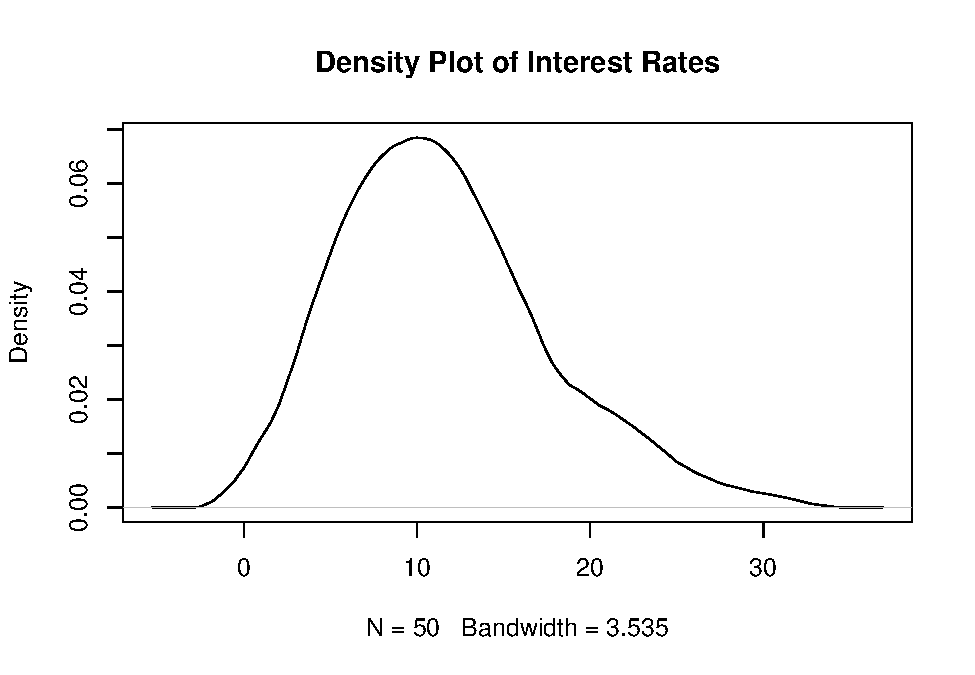
\includegraphics{bookdown-demo_files/figure-latex/4-R2-1.pdf}
\caption{\label{fig:4-R2}Density Plot for 50 Interest Rates, Epanechnikov Kernel, Twice the Bandwidth}
\end{figure}

The density plot in Figure \ref{fig:4-R2} looks smoother than the density plot in Figure \ref{fig:4-R}.

\subsection{Density Plots and Histograms}\label{density-plots-and-histograms}

In Section \ref{densplots}, we mentioned that density plots can be viewed as smoothed versions of a histogram. We create a histogram of interest rates, and overlay a density plot in blue, per Figure \ref{fig:4-R3} below:

\begin{Shaded}
\begin{Highlighting}[]
\FunctionTok{hist}\NormalTok{(Data}\SpecialCharTok{$}\NormalTok{interest\_rate, }\AttributeTok{prob =} \ConstantTok{TRUE}\NormalTok{, }\AttributeTok{main =} \StringTok{"Histogram with Density Plot"}\NormalTok{, }\AttributeTok{xlab=}\StringTok{"Interest Rates"}\NormalTok{)}

\DocumentationTok{\#\#create density plot using default}
\FunctionTok{lines}\NormalTok{(}\FunctionTok{density}\NormalTok{(Data}\SpecialCharTok{$}\NormalTok{interest\_rate), }\AttributeTok{col=}\StringTok{"blue"}\NormalTok{)}
\end{Highlighting}
\end{Shaded}

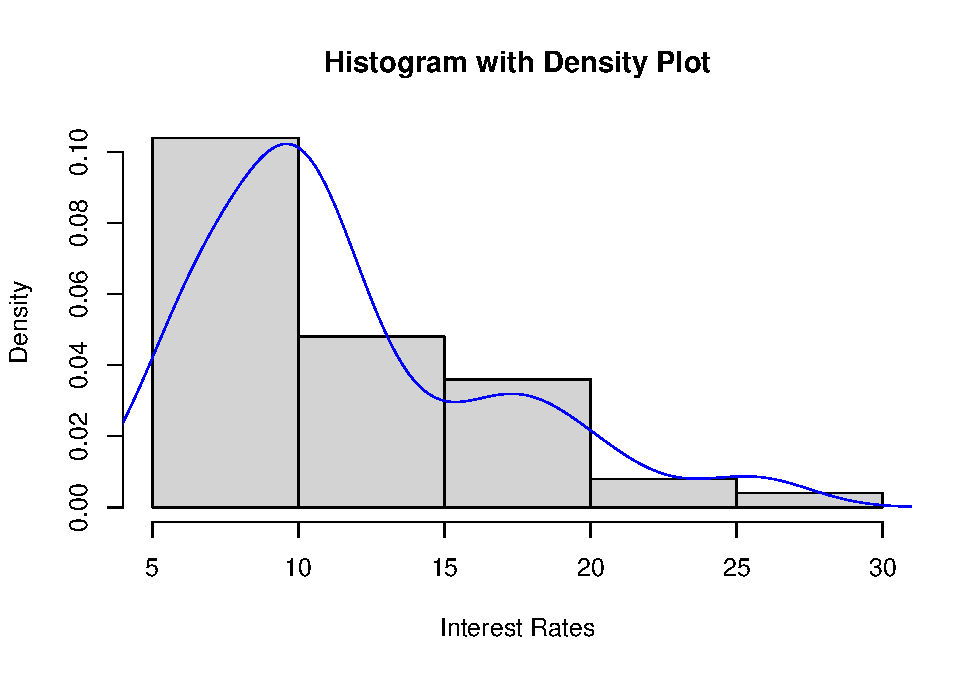
\includegraphics{bookdown-demo_files/figure-latex/4-R3-1.pdf}
Notice how the density plot approximates the histogram.

\subsection{Numerical Summaries}\label{numerical-summaries}

Equations \eqref{eq:4-EX}, \eqref{eq:4-var}, \eqref{eq:4-skew}, and \eqref{eq:4-kurt} are used to obtain the mean, variance, skewness, and kurtosis of a known distribution from a random variable. To calculate these quantities based on a sample of observed data, \(x_1, x_2, \cdots, x_n\), we use:

\begin{equation} 
\bar{x} =  \frac{1}{n} \sum_{i=1}^n x_i,
\label{eq:4-xbar}
\end{equation}

\begin{equation} 
s_X^2 =  \frac{1}{n-1} \sum_{i=1}^n (x_i - \bar{x})^2,
\label{eq:4-sampvar}
\end{equation}

where \(\bar{x}\) and \(s_x^2\) denote the sample mean and variance respectively. The sample skewness and sample kurtosis are

\begin{equation} 
\text{sample skewness } =  \frac{\frac{1}{n} \sum_{i=1}^n (x_i - \bar{x})^3}{s_X^3},
\label{eq:4-sampskew}
\end{equation}

and

\begin{equation} 
\text{sample kurtosis } =  \frac{\frac{1}{n} \sum_{i=1}^n (x_i - \bar{x})^4}{s_X^4} - 3.
\label{eq:4-sampkurt}
\end{equation}

The functions \texttt{mean()}, \texttt{var()}, \texttt{skewness()}, and \texttt{kurtosis()} compute these quantities in R. The latter two functions come from the \texttt{moments} package so be sure to install and load it prior to using them.

\begin{Shaded}
\begin{Highlighting}[]
\FunctionTok{mean}\NormalTok{(Data}\SpecialCharTok{$}\NormalTok{interest\_rate) }\DocumentationTok{\#\#mean}
\end{Highlighting}
\end{Shaded}

\begin{verbatim}
## [1] 11.5672
\end{verbatim}

\begin{Shaded}
\begin{Highlighting}[]
\FunctionTok{var}\NormalTok{(Data}\SpecialCharTok{$}\NormalTok{interest\_rate) }\DocumentationTok{\#\#variance}
\end{Highlighting}
\end{Shaded}

\begin{verbatim}
## [1] 25.52387
\end{verbatim}

\begin{Shaded}
\begin{Highlighting}[]
\FunctionTok{library}\NormalTok{(moments)}
\NormalTok{moments}\SpecialCharTok{::}\FunctionTok{skewness}\NormalTok{(Data}\SpecialCharTok{$}\NormalTok{interest\_rate) }\DocumentationTok{\#\#greater than 0}
\end{Highlighting}
\end{Shaded}

\begin{verbatim}
## [1] 1.102193
\end{verbatim}

\begin{Shaded}
\begin{Highlighting}[]
\NormalTok{moments}\SpecialCharTok{::}\FunctionTok{kurtosis}\NormalTok{(Data}\SpecialCharTok{$}\NormalTok{interest\_rate) }\DocumentationTok{\#\#greater than 0}
\end{Highlighting}
\end{Shaded}

\begin{verbatim}
## [1] 3.651631
\end{verbatim}

So our data is also right skewed and heavy tailed.

\chapter{Joint Distributions}\label{joint-distributions}

This module is based on Introduction to Probability (Blitzstein, Hwang), Chapters 7 and 9. You can access the book for free at \url{https://stat110.hsites.harvard.edu/} (and then click on Book). Please note that I cover additional topics, and skip certain topics from the book. You may skip Story 7.1.9, Theorems 7.1.10 to 7.1.12, Examples 7.1.23 to 7.1.26, Section 7.2, Examples 7.3.6 to 7.3.8, 7.4.8 (parts d and f only), Definition 7.5.6, Examples 9.1.8 to 9.1.10, Example 9.2.5, Theorem 9.3.2, Example 9.3.3, Theorems 9.3.7 to 9.3.9, and Sections 9.4 to 9.6 from the book.

\section{Introduction}\label{introduction-1}

In the previous two modules, we learned how to summarize the distribution of individual random variables. We are now ready to extend the concepts from these modules and apply them to a slightly different setting, where we are analyzing how multiple variables are related to each other. It is extremely common to want to analyze the relationship between at least two variables. The book lists a few examples, but here are a few more:

\begin{itemize}
\tightlist
\item
  Public policy: How does increasing expenditure on infrastructure impact economic development?
\item
  Education: How do smaller class sizes and higher teacher pay impact student learning outcomes?
\item
  Marketing: How does the design of a website influence the probability of a customer purchasing an item?
\end{itemize}

This module will consider these variables jointly, in other words, how they relate to each other. A lot of the concepts such as CDF, PDF, PMF, expectations, variances, and so on will have analogous versions when considering variables jointly.

\section{Joint Distributions for Discrete RVs}\label{joint-distributions-for-discrete-rvs}

We will start with discrete random variables, then move on to continuous random variables. To keep things simple, we will use two random variables to explain concepts. These concepts can then be generalized to any number of random variables.

Recall that for a single discrete random variable \(X\), we use the PMF to inform us the support of \(X\) and the probability associated with each value of the support. We said that the PMF informs us about the distribution of the random variable \(X\).

We now have two discrete random variables, \(X\) and \(Y\). The \textbf{joint distribution} of \(X\) and \(Y\) provides the probability associated with each possible combination of \(X\) and \(Y\). The \textbf{joint PMF} of \(X\) and \(Y\) is

\begin{equation} 
p_{X,Y}(x,y) = P(X=x, Y=y).
\label{eq:5-jointPMF}
\end{equation}

Equation \eqref{eq:5-jointPMF} can be read as the probability that the random variables \(X\) and \(Y\) are equal to \(x\) and \(y\) respectively. Recall that upper case letters are usually used to denote random variables, and lower case letters are usually used as a placeholder for an actual numerical value that the random variable could take.

Joint distributions are sometimes called \textbf{multivariate distributions}. If we are looking at the distribution of one random variable, its distribution can be called a \textbf{univariate distribution}.

Joint PMFs can be displayed via a table, like in Table \ref{tab:simple-table} below. In this example, we consider how study time, \(X\), is related with grades, \(Y\), with

\begin{itemize}
\tightlist
\item
  \(X=1\) for studying 0 to 5 hours a week,
\item
  \(X=2\) for studying 6 to 10 hours a week, and
\item
  \(X=3\) for studying more than 10 hours a week.
\item
  \(Y=1\) denotes getting an A,
\item
  \(Y=2\) denotes getting a B, and
\item
  \(Y=3\) denotes getting a C or lower.
\end{itemize}

\begin{longtable}[]{@{}llll@{}}
\caption{\label{tab:simple-table} Example Joint PMF of Study Time (\(X\)) and Grades (\(Y\))}\tabularnewline
\toprule\noalign{}
& X=1 & X=2 & X=3 \\
\midrule\noalign{}
\endfirsthead
\toprule\noalign{}
& X=1 & X=2 & X=3 \\
\midrule\noalign{}
\endhead
\bottomrule\noalign{}
\endlastfoot
\textbf{Y=1} & 0.05 & 0.15 & 0.30 \\
\textbf{Y=2} & 0.05 & 0.20 & 0.10 \\
\textbf{Y=3} & 0.10 & 0.05 & 0 \\
\end{longtable}

We could also write the joint PMF as:

\begin{itemize}
\tightlist
\item
  \(P(X=1, Y=1) = 0.05\)
\item
  \(P(X=1, Y=2) = 0.05\)
\item
  \(P(X=1, Y=3) = 0.10\)
\item
  \(P(X=2, Y=1) = 0.15\)
\item
  \(P(X=2, Y=2) = 0.20\)
\item
  \(P(X=2, Y=3) = 0.05\)
\item
  \(P(X=3, Y=1) = 0.30\)
\item
  \(P(X=3, Y=2) = 0.10\)
\item
  \(P(X=3, Y=3) = 0\)
\end{itemize}

Just like the PMFs of a single discrete random variable must sum to 1 and each PMF must be non negative, the joint PMFs of discrete random variables must sum to 1 and each individual PMF must be non negative to be valid.

\emph{Thought question}: Can you verify that the joint PMF in Table \ref{tab:simple-table} is valid?

The \textbf{joint CDF} of any discrete random variables \(X\) and \(Y\) is

\begin{equation} 
F_{X,Y}(x,y) = P(X \leq x, Y \leq y).
\label{eq:5-jointCDF}
\end{equation}

\emph{Thought question}: Compare equation \eqref{eq:5-jointCDF} with its univariate counterpart in equation \eqref{eq:3-CDF}. Can you see the similarities and differences?

\subsection{Marginal Distributions for Discrete RVs}\label{marginal-distributions-for-discrete-rvs}

From the joint distribution of \(X\) and \(Y\), we can get the distribution of each individual random variable. We call this the \textbf{marginal distribution}, or unconditional distribution, of \(X\) and \(Y\). The marginal distribution of \(X\) gives us information about the distribution of \(X\), without taking \(Y\) into consideration. To get the marginal PMF of \(X\) from the joint PMF of \(X\) and \(Y\):

\begin{equation} 
P(X=x) = \sum_y P(X=x, Y=y).
\label{eq:5-margPMF}
\end{equation}

Note that the summation is performed over the support of \(Y\). We go back to Table \ref{tab:simple-table} as an example. Suppose we want to find the marginal distribution of study times, \(X\). Applying equation \eqref{eq:5-margPMF}:

\[
\begin{split}
P(X=1) &= \sum_y P(X=1, Y=y)\\
 &= P(X=1, Y=1) + P(X=1, Y=2) + P(X=1, Y=3) \\
&= 0.05 + 0.05 + 0.10\\
&= 0.2,
\end{split}
\]

\[
\begin{split}
P(X=2) &= \sum_y P(X=2, Y=y)\\
 &= P(X=2, Y=1) + P(X=2, Y=2) + P(X=2, Y=3) \\
&= 0.15 + 0.20 + 0.05\\
&= 0.4,
\end{split}
\]

and

\[
\begin{split}
P(X=3) &= \sum_y P(X=3, Y=y)\\
 &= P(X=3, Y=1) + P(X=3, Y=2) + P(X=3, Y=3) \\
&= 0.30 + 0.10 + 0\\
&= 0.4.
\end{split}
\]

We can add this information to Table \ref{tab:simple-table}, to create Table \ref{tab:5-marg-table}

\begin{longtable}[]{@{}llll@{}}
\caption{\label{tab:5-marg-table} Example Joint PMF of Study Time (\(X\)) and Grades (\(Y\)), with Marginal PMF of Study Time}\tabularnewline
\toprule\noalign{}
& X=1 & X=2 & X=3 \\
\midrule\noalign{}
\endfirsthead
\toprule\noalign{}
& X=1 & X=2 & X=3 \\
\midrule\noalign{}
\endhead
\bottomrule\noalign{}
\endlastfoot
\textbf{Y=1} & 0.05 & 0.15 & 0.30 \\
\textbf{Y=2} & 0.05 & 0.20 & 0.10 \\
\textbf{Y=3} & 0.10 & 0.05 & 0 \\
\textbf{Total} & 0.2 & 0.4 & 0.4 \\
\end{longtable}

Notice we just added the probabilities in each column to get the marginal PMF of \(X\), and write these probabilities to the margin of the table (hence the term marginal PMF).

You may notice that the marginal PMF of \(X\) ends up being just the PMF of \(X\). The term marginal is used to imply that the PMF was derived from a joint PMF, even if the information is the same.

\emph{Thought question}: Can you see how equation \eqref{eq:5-margPMF} is based on the Law of Total Probability in equation \eqref{eq:total}?

View the video below for a more detailed explanation on deriving the marginal PMF of \(X\):

Likewise, to obtain the marginal PMF of \(Y\) from the joint PMF of \(X\) and \(Y\):

\begin{equation} 
P(X=x) = \sum_x P(X=x, Y=y).
\label{eq:5-margPMF2}
\end{equation}

The summation is now performed over the support of \(X\).

\emph{Thought question}: Can you verify the marginal PMF for grades displayed Table \ref{tab:5-marg-table2} below?

\begin{longtable}[]{@{}lllll@{}}
\caption{\label{tab:5-marg-table2} Example Joint PMF of Study Time (\(X\)) and Grades (\(Y\)), with Marginal PMF of Study Time and Study Time}\tabularnewline
\toprule\noalign{}
& X=1 & X=2 & X=3 & Total \\
\midrule\noalign{}
\endfirsthead
\toprule\noalign{}
& X=1 & X=2 & X=3 & Total \\
\midrule\noalign{}
\endhead
\bottomrule\noalign{}
\endlastfoot
\textbf{Y=1} & 0.05 & 0.15 & 0.30 & 0.50 \\
\textbf{Y=2} & 0.05 & 0.20 & 0.10 & 0.35 \\
\textbf{Y=3} & 0.10 & 0.05 & 0 & 0.15 \\
\textbf{Total} & 0.2 & 0.4 & 0.4 & 1 \\
\end{longtable}

\subsection{Conditional Distributions for Discrete RVs}\label{conddist}

We may need to update the distribution of one of the variables based on the observed value of the other variable, or we need the distribution of one of the variables based on a specific value of the other variable. This leads to the \textbf{conditional PMF}.

Suppose we want to update the distribution of \(Y\) based on the observed value \(X=x\), or we want the distribution of \(Y\) only for observations where \(X=x\) (or in other words, \(X\) is equal to a specific value \(x\)). If \(X\) and \(Y\) are both discrete, the conditional PMF of \(Y\) given \(X=x\) is:

\begin{equation} 
P(Y=y|X=x) = \frac{P(X=x, Y=y)}{P(X=x)}.
\label{eq:5-condPMFY}
\end{equation}

The conditional PMF of \(Y\) given \(X=x\) is essentially the joint PMF of \(X\) and \(Y\) divided by the marginal PMF of \(X\). Note that the conditional PMF of \(Y\) given \(X=x\) is viewed as a function with the value of \(x\) being fixed.

We go back to Table \ref{tab:simple-table} as an example on how to find conditional PMFs. Suppose we want to find the distribution of grades for students who study little (0 to 5 hours per week). We want the conditional PMF of \(Y\) given that \(X=1\). Applying equation \eqref{eq:5-condPMFY} to Table \ref{tab:5-marg-table2}, we have

\[
\begin{split}
P(Y=1|X=1) &= \frac{P(X=1, Y=1)}{P(X=1)}\\
 &= \frac{0.05}{0.2} \\
&= 0.25,
\end{split}
\]

\[
\begin{split}
P(Y=2|X=1) &= \frac{P(X=1, Y=2)}{P(X=1)}\\
 &= \frac{0.05}{0.2} \\
&= 0.25,
\end{split}
\]

and

\[
\begin{split}
P(Y=3|X=1) &= \frac{P(X=1, Y=3)}{P(X=1)}\\
 &= \frac{0.10}{0.2} \\
&= 0.5.
\end{split}
\]
The frequentist interpretation of these values is that among the students who studied little, they have a 50\% chance of getting a C or lower, a 25\% chance of getting a B, and a 25\% chance of getting an A.

The Bayesian interpretation of these values is that if I know the student studied little, the student has a 50\% chance of getting a C or lower, a 25\% chance of getting a B, and a 25\% chance of getting an A.

\emph{Thought question}: Can you show the conditional PMF of \(Y\) given \(X=3\) based on Table \ref{tab:5-marg-table2} is \(P(Y=1|X=3) = 0.75, P(Y=2|X=3) = 0.25, P(Y=3|X=3) = 0\)?

To find the conditional PMF of \(X\) given \(Y=y\):

\begin{equation} 
P(X=x|Y=y) = \frac{P(X=x, Y=y)}{P(Y=y)}.
\label{eq:5-condPMFX}
\end{equation}

\emph{Thought question}: Can you show the conditional PMF of \(X\) given \(Y=1\) based on Table \ref{tab:5-marg-table2} is \(P(X=1|Y=1) = 0.1, P(X=2|Y=1) = 0.3, P(X=3|Y=1) = 0.6\)?

\subsection{Bayes' Rule}\label{bayes-rule-1}

We can apply Bayes' Rule for an alternative way of finding the conditional PMF of \(Y\) given \(X=x\). Equation \eqref{eq:5-condPMFY} can be written as:

\begin{equation} 
P(Y=y|X=x) = \frac{P(X=x|Y=y) P(Y=y)}{P(X=x)}.
\label{eq:5-condPMFbayes}
\end{equation}

\subsection{Law of Total Probability}\label{law-of-total-probability-1}

We can apply the law of total probability to the denominator of equations \eqref{eq:5-condPMFY} and \eqref{eq:5-condPMFbayes}, i.e.~\(P(X=x) = \sum_y P(X=x|Y=y) P(Y=y)\), so the conditional PMF of \(Y\) given \(X=x\) can also be written as

\begin{equation} 
P(Y=y|X=x) = \frac{P(X=x|Y=y) P(Y=y)}{\sum_y P(X=x|Y=y) P(Y=y)}.
\label{eq:5-condPMFtotal}
\end{equation}

\subsection{Indepdence of Discrete RVs}\label{indepdence-of-discrete-rvs}

The notion of whether two random variables are \textbf{independent} or not (also called dependent) is whether the random variables have an association, or in other words, does changing the value of one random variable affect the distribution of the other?

If \(X\) and \(Y\) are discrete random variables, they are independent only if, for all values in the support of \(X\) and \(Y\):

\begin{equation} 
P(X=x, Y=y) = P(X=x) P(Y=y).
\label{eq:5-ind}
\end{equation}

An equivalent condition is that for all values in the support of \(X\) and \(Y\):

\begin{equation} 
P(Y=y | X=x) = P(Y=y),
\label{eq:5-ind2}
\end{equation}

or

\begin{equation} 
P(X=x | Y=y) = P(X=x),
\label{eq:5-ind3}
\end{equation}

To show that \(X\) and \(Y\) are independent, we need to show one of equations \eqref{eq:5-ind}, \eqref{eq:5-ind2}, or \eqref{eq:5-ind3} to be true for \textbf{all values in the support} of \(X\) and \(Y\). To show that \(X\) and \(Y\) are dependent, we need to show one of equations \eqref{eq:5-ind}, \eqref{eq:5-ind2}, or \eqref{eq:5-ind3} to be false for \textbf{just one value} of \(X\) and \(Y\).

Equations \eqref{eq:5-ind2} and \eqref{eq:5-ind3} are pretty intuitive. These equations say that the conditional distribution of one variable, given the other, is the same as the marginal distribution of the variable. This means the distribution of the variable is not influenced by knowledge about the other variable.

The first equation \eqref{eq:5-ind} informs us that if the discrete variables are independent, their joint PMF is equal to the product of their marginal PMFs.

We go back to the study time and grades example shown in Table \ref{tab:5-marg-table2}. Study time and grades are dependent (or not independent) since \(P(Y=1|X=1) = 0.25\) but \(P(Y=1) = 0.5\). They are not equal so study time and grades are not independent. It is usually easier to prove a condition is not met by providing a \textbf{counterexample}: find one specific example where the condition is false.

If study time and grades were independent, we needed to show \(P(Y=1|X=x) = P(Y=1)\) when \(X=1,2,3\), \(P(Y=2|X=x) = P(Y=2)\) when \(X=1,2,3\), and \(P(Y=3|X=x) = P(Y=3)\) when \(X=1,2,3\). It is usually more tedious to prove a condition is met as we have to show the condition is met under all circumstances.

Very often, knowing the context of the random variables helps. Since we expect students who study more to get better grades, we expect these variables to be dependent, so we know we just need to provide a counterexample.

\section{Joint, Marginal, Conditional Distributions for Continuous RVs}\label{joint-marginal-conditional-distributions-for-continuous-rvs}

Recall in the previous modules the CDFs and PDFs for a continuous random variable are similar to CDFs and PMFs for discrete random variables. The continuous versions are generally found by swapping summations with integrals. The same general idea applies with joint distributions when both random variables are continuous.

Now suppose that \(X\) and \(Y\) denote random variables that are continuous. It is required that the \textbf{joint CDF} \(F_{X,Y}(x,y) = P(X \leq x, Y \leq y)\) is differentiable with respect to \(x\) and \(y\). Their \textbf{joint PDF} is the partial derivative of their joint CDF with respect to \(x\) and \(y\): \(f_{X,Y}(x,y) = \frac{\partial^2}{\partial x \partial y} F_{X,Y}(x,y)\).

Similar to univariate PDFs, for joint PDFs to be valid, we require that:

\begin{itemize}
\tightlist
\item
  \(f_{X,Y}(x,y) \geq 0\) and
\item
  \(\int_{-\infty}^\infty \int_{-\infty}^\infty f_{X,Y}(x,y)  dx dy = 1\).
\end{itemize}

To find probabilities, for example \(P(a<X<b, c<Y<d)\), we integrate the joint PDF over the two-dimensional region, i.e.~\(\int_{c}^d \int_{a}^b f_{X,Y}(x,y) dx dy\).

The \textbf{marginal PDF} of \(X\) can be found by integrating their joint PDF over the support of \(Y\):

\begin{equation} 
f_X(x) = \int_{-\infty}^\infty f_{X,Y}(x,y) dy.
\label{eq:5-margPDF}
\end{equation}

The conditional PDF of \(Y\) given \(X=x\) is

\begin{equation} 
f_{Y|X}(y|x) = \frac{f_{X,Y}(x,y)}{f_X(x)}
\label{eq:5-condPDF}
\end{equation}

Bayes' rule for continuous random variables is

\begin{equation} 
f_{Y|X}(y|x) = \frac{f_{X|Y}(x|y) f_Y(y)}{f_X(x)}
\label{eq:5-condPDFbayes}
\end{equation}

And the law of total probability is

\begin{equation} 
f_X(x) = \int_{-\infty}^\infty f_{X|Y}(x|y) f_Y(y) dy.
\label{eq:5-condPDFtotal}
\end{equation}

Continuous random variables \(X\) and \(Y\) are independent if for all values of \(x\) and \(y\):

\begin{equation} 
F_{X,Y} (x,y) = F_X(x) F_Y(y)
\label{eq:5-indcont1}
\end{equation}

or

\begin{equation} 
f_{X,Y} (x,y) = f_X(x) f_Y(y)
\label{eq:5-indcont2}
\end{equation}

or

\begin{equation} 
f_{Y|X} (y|x) = f_Y(y)
\label{eq:5-indcont3}
\end{equation}

or

\begin{equation} 
f_{X|Y} (x|y) = f_X(x).
\label{eq:5-indcont4}
\end{equation}

\section{Covariance and Correlation}\label{covariance-and-correlation}

In the previous modules, we used summaries such as the mean, variance, skewness, and kurtosis to provide some insight into the distribution of a single random variable. When we have multiple random variables, one question we have is how are the random variables related to each other. Summaries that are used to quantify the \textbf{linear relationship} between two quantitative random variables are the covariance and correlation.

Generally speaking, two random variables have a positive covariance and correlation if they increase or decrease together, i.e.~if \(X\) increases, \(Y\) also generally increases; if \(X\) decreases, \(Y\) also generally decreases.

Two random variables have a negative covariance and correlation if they move in the opposite direction, i.e.~if \(X\) increases, \(Y\) generally decreases; if \(X\) decreases, \(Y\) generally increases. Figure \ref{fig:5-covs} below displays these ideas visually through scatter plots. The scatter plot on the left shows an example of a pair of random variables having positive covariance, and the scatter plot on the right shows an example of a pair of random variables having negative covariance.

\begin{figure}
\centering
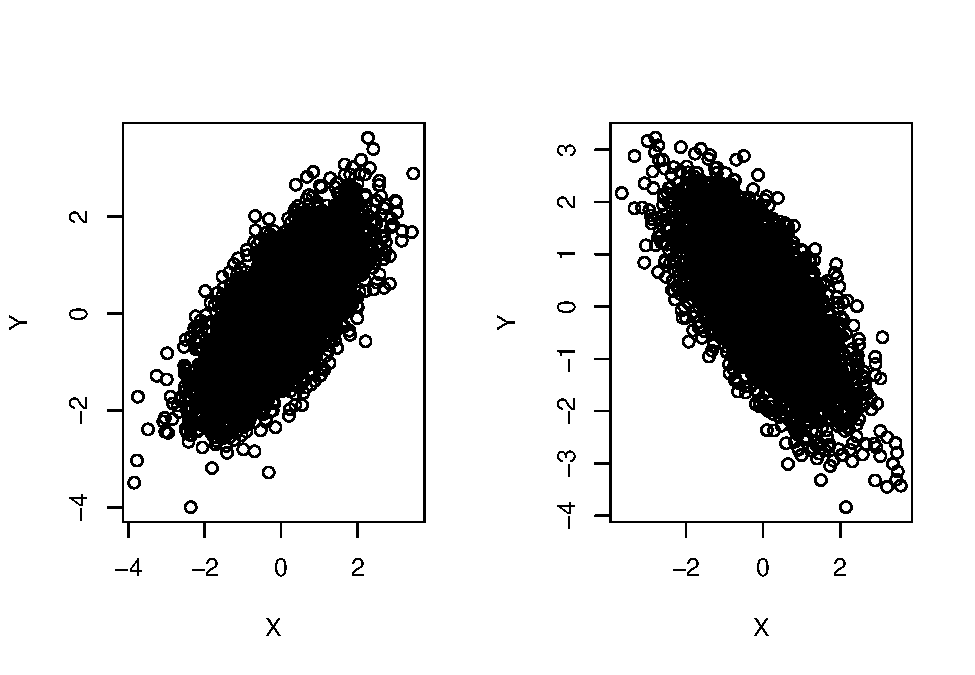
\includegraphics{bookdown-demo_files/figure-latex/5-covs-1.pdf}
\caption{\label{fig:5-covs}Positive Covariance (Left), Negative Covariance (Right)}
\end{figure}

One more thing to note: covariance and correlations can be calculated for random variables as long as they are quantitative, but not if at least one of them is categorical. The concept of increasing a random variable that is categorical does not make intuitive sense, for example, if we have a random variable that denotes the color of eyes, what does increasing color of eyes mean?

\subsection{Covariance}\label{5-cov}

We now define covariance. The \textbf{covariance} between random variables \(X\) and \(Y\) is

\begin{equation} 
Cov(X,Y) = E\left[(X- \mu_X)(Y - \mu_Y) \right].
\label{eq:5-cov}
\end{equation}

Looking at equation \eqref{eq:5-cov}, we see that if both \(X\) and \(Y\) generally move in the same direction, then \(X - \mu_x\) and \(Y - \mu_y\) will either be both positive or both negative, therefore their product is positive, on average. If \(X\) and \(Y\) generally move in opposite directions, then \(X - \mu_x\) and \(Y - \mu_y\) have opposite signs, therefore their product is negative, on average.

Some key properties for covariance:

\begin{itemize}
\tightlist
\item
  \(Cov(X,X) = Var(X)\).The covariance of any random variable with itself is its variance.
\item
  \(Cov(X,Y) = Cov(Y,X)\). The covariance between \(X\) and \(Y\) is the same as the covariance between \(Y\) and \(X\).
\item
  \(Cov(X,c) = 0\) for any constant \(c\). Since a constant does not move, it has no relationship with \(X\).
\item
  \(Cov(aX,Y) = a Cov(X,Y)\) for any constant \(a\). This implies that covariance is affected by the units of \(X\) and \(Y\).
\item
  \(Var(X + Y) = Var(X) + Var(Y) + 2 Cov(X,Y)\).
\item
  If \(X\) and \(Y\) are independent, then \(Cov(X,Y) = 0\).
\item
  However, \(Cov(X,Y) = 0\) does not mean that \(X\) and \(Y\) are independent. This is a common misconception. Remember that covariance measures linear relationship. The relationship between \(X\) and \(Y\) could be non linear, and in such instances, the covariance should not be used. Figure \ref{fig:5-cov0} below provides an example this. In this figure, \(X\) and \(Y\) have a quadratic relationship, so they are clearly not independent, yet their covariance is virtually 0.
\end{itemize}

\begin{Shaded}
\begin{Highlighting}[]
\NormalTok{x}\OtherTok{\textless{}{-}}\FunctionTok{seq}\NormalTok{(}\SpecialCharTok{{-}}\DecValTok{1}\NormalTok{,}\DecValTok{1}\NormalTok{, }\AttributeTok{by=}\FloatTok{0.01}\NormalTok{)}
\NormalTok{y}\OtherTok{\textless{}{-}}\NormalTok{x}\SpecialCharTok{\^{}}\DecValTok{2}

\DocumentationTok{\#\#note from plot that X \& Y do not have a linear relationship}
\FunctionTok{plot}\NormalTok{(x,y, }\AttributeTok{xlab=}\StringTok{"X"}\NormalTok{, }\AttributeTok{ylab=}\StringTok{"Y"}\NormalTok{)}
\end{Highlighting}
\end{Shaded}

\begin{figure}
\centering
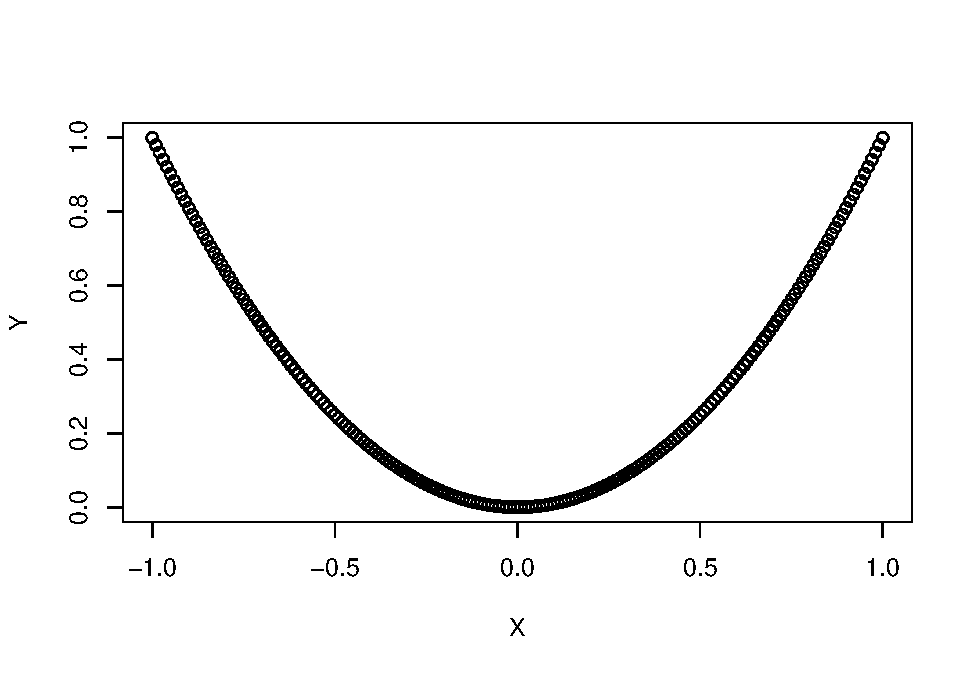
\includegraphics{bookdown-demo_files/figure-latex/5-cov0-1.pdf}
\caption{\label{fig:5-cov0}Covariance with Non Linear Relationship}
\end{figure}

\begin{Shaded}
\begin{Highlighting}[]
\FunctionTok{cov}\NormalTok{(x,y) }\DocumentationTok{\#\#covariance is virtually 0}
\end{Highlighting}
\end{Shaded}

\begin{verbatim}
## [1] 1.19967e-17
\end{verbatim}

Suppose we have two vectors of observed data, each of size \(n\): \(X = (x_1, x_2, \cdots, x_n)\) and \(Y = (y_1, y_2, \cdots, y_n)\). Their \textbf{sample covariance} is

\begin{equation} 
s_{x,y} = \frac{\sum_{i=1}^n (x_i - \bar{x})(y_i - \bar{y})}{n-1}
\label{eq:5-sampcov}
\end{equation}

We noted earlier that covariance is affected by the units of the variables. Suppose one variable is measured in meters, and we convert it to become centimeters. The value of the covariance will get multiplied by 100. People find it easier to interpret a measure that does not depend on the units. This is where the correlation comes in: it is a unitless version of the covariance.

View the video below for a visual explanation as to why the sample covariance is positive when the linear relationship is positive:

\subsection{Correlation}\label{correlation}

The \textbf{correlation} between random variables \(X\) and \(Y\) is

\begin{equation} 
\rho = Corr(X,Y) = \frac{Cov(X,Y)}{\sqrt{Var(X) Var(Y)}}.
\label{eq:5-corr}
\end{equation}

The \textbf{sample correlation} for two vectors of observed data, each of size \(n\): \(X = (x_1, x_2, \cdots, x_n)\) and \(Y = (y_1, y_2, \cdots, y_n)\), is

\begin{equation} 
r = \frac{\sum_{i=1}^n (x_i - \bar{x})(y_i - \bar{y})}{\sqrt{\sum_{i=1}^n (x_i - \bar{x})^2 \sum_{i=1}^n (y_i - \bar{y})^2}}
\label{eq:5-sampcorr}
\end{equation}

Some key properties of correlation:

\begin{itemize}
\tightlist
\item
  It is bounded between -1 and 1.
\item
  Values closer to -1 or 1 indicate a stronger linear relationship.
\item
  Values closer to 0 indicate a weaker linear relationship.
\item
  Its numerical value is unchanged with location and / or scale changes.
\item
  If \(X\) and \(Y\) are independent, then \(Corr(X,Y) = 0\).
\item
  However, \(Corr(X,Y) = 0\) does not mean that \(X\) and \(Y\) are independent.
\item
  Correlation should only be used if the relationship between \(X\) and \(Y\) is linear.
\end{itemize}

Figure \ref{fig:5-corrs} below shows examples of some scatterplots and their sample correlations. For the left plot, the data points fall close to a straight line, is negative, and so its correlation is close to -1. The middle plot has no linear relationship, so we do not see a trend with one variable increasing or decreasing as the other variable increases. The right plot shows the data points being fairly close to a straight line, but not as close as the left plot), so its correlation is not as close to 1 (or -1).

\begin{figure}
\centering
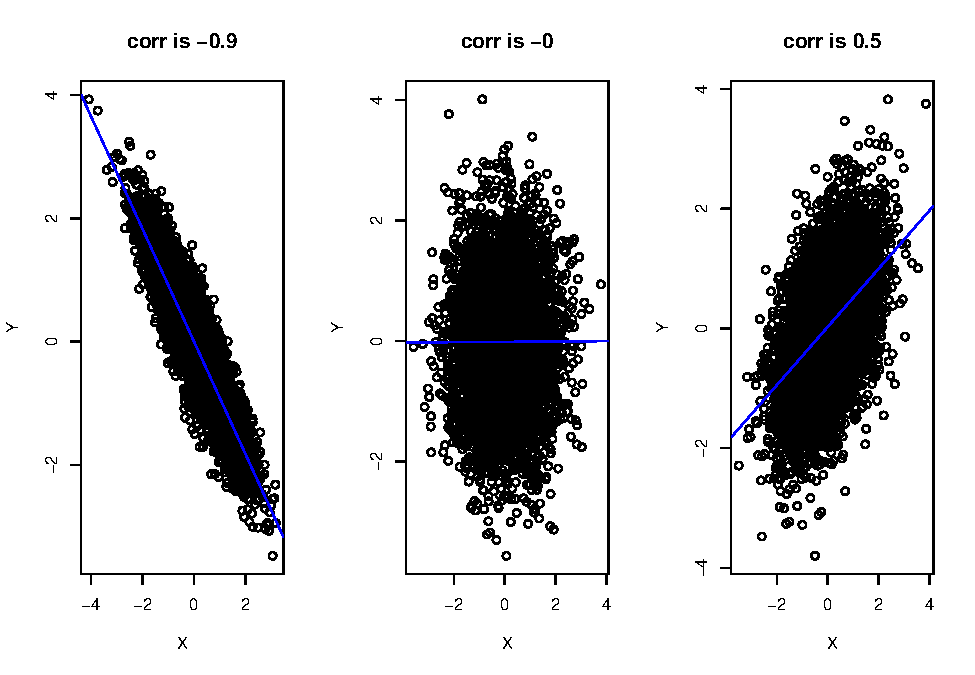
\includegraphics{bookdown-demo_files/figure-latex/5-corrs-1.pdf}
\caption{\label{fig:5-corrs}Strong Negative Correlation (Left), No Correlation (Middle), Moderate Positive Correlation (Right)}
\end{figure}

\section{Conditional Expectation}\label{conditional-expectation}

In Section \ref{condprob} and \ref{conddist}, we explored the notion of conditional probabilities and conditional distributions, which are used for:

\begin{itemize}
\tightlist
\item
  Updating the probability and distribution of a random variable \(Y\), after observing a certain outcome of another random variable \(X\), or
\item
  Restricting the probability and distribution of a random variable \(Y\) to a certain value of another random variable.
\end{itemize}

These represent the Bayesian and frequentist viewpoints of conditional probability and conditional distribution.

It turns out a similar idea applies to the expected value of a random variable. Recall that the expected value of a random variable is the long-run average, in other words, the average value after observing the random variable an infinite number of times.

The conditional expectation of a random variable is its long run-average:

\begin{itemize}
\tightlist
\item
  after observing a certain outcome of another variable or event, or
\item
  after restricting our attention to cases when another random variable is fixed or equal to a specific value.
\end{itemize}

Fairly often, we use statistical models to predict a response variable \(Y\) based on a predictor \(X\). Predictions for values of \(Y\) based on observed values of \(X\) usually use the conditional expectation of \(Y\) given \(X\). Given what we see with the predictor, the long run average of \(Y\) ends up being used as the predicted value of the response variable. This is the basis for most statistical models.

There are two slightly different notions of conditional expectations:

\begin{itemize}
\tightlist
\item
  Conditional expectation of random variable \(Y\) given event \(A\). If \(A\) has happened, what is the expected value of \(Y\)?
\item
  Conditional expectation of random variable \(Y\) given another random variable \(X\). If we fix the value of the random variable \(X\) to any value on its support, what is the expected value of \(Y\)?
\end{itemize}

The second notion is the one that is usually used for statistical models, but we will cover both as the first notion is easier to understand, and should help us understand the second notion.

\subsection{Conditional Expectation Given Event}\label{conditional-expectation-given-event}

Recall that the expectation \(E(Y)\) of a random variable \(Y\) is its long-run average. If \(Y\) is discrete, we take a weighted average involving the probabilities in its PMF \(P(Y=y)\). The calculation of the \textbf{conditional expectation} \(E(Y|A)\) where \(A\) is an event that has occurred simply replaces the probabilities \(P(Y=y)\) with conditional probabilities \(P(Y=y|A)\). Therefore, for a discrete random variable \(Y\),

\begin{equation} 
E(Y|A) = \sum_y y P(Y=y|A) 
\label{eq:5-condexpdis}
\end{equation}

where the sum is over the support of \(Y\). Notice how we are summing the product of the support with its corresponding conditional probability, whereas to find \(E(Y)\), we sum the product of the support with its corresponding unconditional probability.

If \(Y\) is continuous, we use the conditional PDF instead:

\begin{equation} 
E(Y|A) = \int_{-\infty}^{\infty} y f(y|A) dy.
\label{eq:5-condexpcont}
\end{equation}

The key is to understand the intuition behind conditional expectations, and we will use simulation to approximate this (the approximation works better if we use more simulated data). Simulation represents the frequentist viewpoint of conditional expectation. The code below does the following:

\begin{itemize}
\tightlist
\item
  Generate 100 values of \(X\) uniformly on the support \(\{1,2,3,4\}\).
\item
  Simulate \(Y\) using \(Y = 10 + X + \epsilon\) where \(\epsilon \sim N(0,1)\).
\item
  Represent these values on a scatter plot, and also overlay a line that represents the sample mean of \(Y\), which estimates \(E(Y)\). This is simply the average value on the y-axis for all 100 data points. This is the plot on the left in Figure \ref{fig:5-condexp} below.
\item
  Represent these values on a scatter plot, but use blue to denote the event \(A\) which is when \(X=1\). A line that represents the sample mean of \(Y\), only for these blue data points (i.e.~only when \(X=1\)), is overlaid. This value estimates \(E(Y|A)\) or \(E(Y|X=1)\). This is the plot on the right in Figure \ref{fig:5-condexp} below. In calculating this sample mean, we could have completed disregarded the black data points when \(X\) was not 1.
\end{itemize}

\begin{Shaded}
\begin{Highlighting}[]
\FunctionTok{set.seed}\NormalTok{(}\DecValTok{40}\NormalTok{)}
\NormalTok{n}\OtherTok{\textless{}{-}}\DecValTok{100} \DocumentationTok{\#\#100 data points}

\DocumentationTok{\#\#generate X}
\NormalTok{x}\OtherTok{\textless{}{-}}\FunctionTok{c}\NormalTok{(}\FunctionTok{rep}\NormalTok{(}\DecValTok{1}\NormalTok{,n}\SpecialCharTok{/}\DecValTok{4}\NormalTok{), }\FunctionTok{rep}\NormalTok{(}\DecValTok{2}\NormalTok{,n}\SpecialCharTok{/}\DecValTok{4}\NormalTok{), }\FunctionTok{rep}\NormalTok{(}\DecValTok{3}\NormalTok{,n}\SpecialCharTok{/}\DecValTok{4}\NormalTok{), }\FunctionTok{rep}\NormalTok{(}\DecValTok{4}\NormalTok{,n}\SpecialCharTok{/}\DecValTok{4}\NormalTok{)) }

\DocumentationTok{\#\#simulate Y}
\NormalTok{y}\OtherTok{\textless{}{-}} \DecValTok{10} \SpecialCharTok{+}\NormalTok{ x }\SpecialCharTok{+} \FunctionTok{rnorm}\NormalTok{(n)}

\FunctionTok{par}\NormalTok{(}\AttributeTok{mfrow=}\FunctionTok{c}\NormalTok{(}\DecValTok{1}\NormalTok{,}\DecValTok{2}\NormalTok{))}
\FunctionTok{plot}\NormalTok{(x,y, }\AttributeTok{main=}\StringTok{"Estimated E(Y) Overlaid"}\NormalTok{)}
\FunctionTok{abline}\NormalTok{(}\AttributeTok{h=}\FunctionTok{mean}\NormalTok{(y)) }\DocumentationTok{\#\#add line to represent est E(Y)}

\FunctionTok{plot}\NormalTok{(x,y, }\AttributeTok{col =} \FunctionTok{ifelse}\NormalTok{(x }\SpecialCharTok{==} \DecValTok{1}\NormalTok{,}\StringTok{\textquotesingle{}blue\textquotesingle{}}\NormalTok{, }\StringTok{\textquotesingle{}black\textquotesingle{}}\NormalTok{), }\AttributeTok{pch =} \DecValTok{19}\NormalTok{, }\AttributeTok{main=}\StringTok{"Estimated E(Y|X=1) Overlaid"}\NormalTok{ )}
\FunctionTok{abline}\NormalTok{(}\AttributeTok{h=}\FunctionTok{mean}\NormalTok{(y[}\AttributeTok{x=}\DecValTok{1}\NormalTok{]), }\AttributeTok{col=}\StringTok{"blue"}\NormalTok{) }\DocumentationTok{\#\#add line to represent est E(Y|X=1)}
\end{Highlighting}
\end{Shaded}

\begin{figure}
\centering
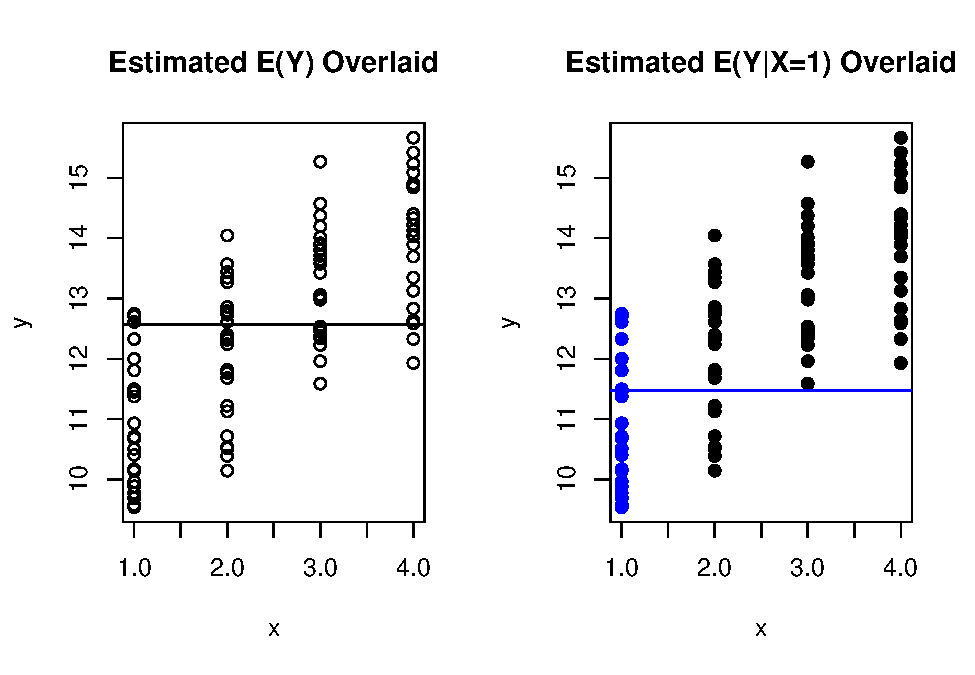
\includegraphics{bookdown-demo_files/figure-latex/5-condexp-1.pdf}
\caption{\label{fig:5-condexp}Comparison of E(Y) and E(Y\textbar X=1)}
\end{figure}

So, we can interpret the conditional expectation \(E(Y|A)\) as the long-run average of \(Y\) (only) when \(A\) has happened. It is the long-run average of \(Y\) when a certain condition is met.

View the video below for a more detailed explanation for this simulation:

\subsection{Conditional Expectation Given Random Variable}\label{conditional-expectation-given-random-variable}

The conditional expectation of \(Y\) given a random variable \(X\) is slightly different. In the simulated example in the previous subsection, we set \(X\) to be a specific value. Now, we consider the long-run average of \(Y\) for each value, instead of a specific value, in the support of \(X\).

One way to think about this is to consider \(E(Y|X=x)\), where \(x\) is any value on the support for \(X\). If \(Y\) is discrete, this conditional expectation is:

\begin{equation} 
E(Y|A) = \sum_y y P(Y=y|X=x) 
\label{eq:5-condexpdis2}
\end{equation}

where the sum is over the support of \(Y\).

If \(Y\) is continuous:

\begin{equation} 
E(Y|A) = \int_{-\infty}^{\infty} y f(y|x) dy.
\label{eq:5-condexpcont2}
\end{equation}

We go back to the simulated example in the previous subsection to explain what \(E(Y|X=x)\) represents. Recall that the support for \(X\) is \(\{1,2,3,4\}\) and that \(Y = 10 + X + \epsilon\) where \(\epsilon \sim N(0,1)\). So

\[
\begin{split}
E(Y|X=x) &= E(10 + X + \epsilon | X=x)\\
 &= E(10 + x + \epsilon) \\
 &= E(10) + E(x) + E(\epsilon) \\
&= 10 + x + 0 \\
 &= 10 + x.
\end{split}
\]

A brief explanation of each step:

\begin{itemize}
\tightlist
\item
  To go from line 1 to line 2, we subbed in \(x\) for \(X\), since we are setting \(X=x\).
\item
  To go from line 2 to line 3, we apply the linearity of expectations.
\item
  To go from line 3 to 4, \(E(c)=c\) for any constant. In this case, we are fixing \(x\) to be a value in the support so it is a constant, and \(E(\epsilon) = 0\) since \(\epsilon \sim N(0,1)\).
\end{itemize}

So \(E(Y|X) = 10 + X\). What this means is that:

\begin{itemize}
\tightlist
\item
  When \(X=1\), \(E(Y|X=1) = 11\),
\item
  When \(X=2\), \(E(Y|X=1) = 12\),
\item
  When \(X=3\), \(E(Y|X=1) = 13\), and
\item
  When \(X=4\), \(E(Y|X=1) = 14\).
\end{itemize}

Note: We set up \(Y = 10 + X + \epsilon\) where \(\epsilon \sim N(0,1)\) in the simulation. This follows the framework for linear regression which sets up \(Y = \beta_0 + \beta_1 X + \epsilon\) where \(\epsilon \sim N(0,\sigma^2)\), i.e.~\(\epsilon\) is normal with mean 0 and a variance that is a fixed value. The conditional expectation given \(X\) ends up being the prediction for \(Y\) that minimizes the mean squared error in linear regression.

View the video below for a more detailed explanation of this example:

\section{Common Multivariate Distributions}\label{common-multivariate-distributions}

We now cover two of the most common multivariate distributions: the multinomial distribution and multivariate normal distribution for discrete and continuous random variables respectively.

\subsection{Multinomial}\label{multinomial}

The \textbf{multinomial} distribution can be viewed as a generalization of the binomial distribution into higher dimensions. Recall that for the binomial distribution, we carry out \(n\) trials, and for each trial we record whether it as a success or failure, in other words, there are only two outcomes for each trial. The multinomial distribution differs in that there can be more than two outcomes for each trial. For example, we randomly select \(n\) adults and ask them for their political affiliation. The affiliation could be Democrat, Republican, other party, or no affiliation, so there are four possible outcomes or categories for each person.

The set up of the multinomial distribution is as follows:

\begin{itemize}
\tightlist
\item
  We have \(n\) independent trials, and each trial belongs to one of \(k\) categories.
\item
  Each trial belongs to category \(j\) with probability \(p_j\), where \(p_j\) is non negative and \(\sum_{j=1}^k p_j = 1\), i.e.~they sum to one.
\item
  Let \(X_1\) denote the number of trials belonging to category 1, \(X_2\) denote the number of trials belonging to category 2, and so on. Then \(X_1 + \cdots X_k = n\).
\end{itemize}

We then say that \(\boldsymbol{X} = (X_1, \cdots, X_k)\) is said to have a multinomial distribution with parameters \(n\) and \(\boldsymbol{p} = (p_1, \cdots, p_k)\). This can be written as \(\boldsymbol{X} \sim Mult_k(n, \boldsymbol{p})\).

Note that the vectors \(\boldsymbol{X}\) and \(\boldsymbol{p}\) are written in bold. Vectors and matrices are commonly written using bold to distinguish them from scalars, which are not in bold. \(\boldsymbol{X}\) is an example of what we call a random vector, as it is a vector of random variables \(X_1, \cdots, X_k\).

If \(\boldsymbol{X} \sim Mult_k(n, \boldsymbol{p})\), its PMF is

\begin{equation} 
P(X_1 = n_1, \cdots, X_k = n_k) = \frac{n!}{n_{1}! \cdots n_{k}!} p_1^{n_1} \cdots p_k^{n_k},
\label{eq:5-multinomial}
\end{equation}

where \(n_1 + \cdots + n_k = n\).

Let us use a toy example. Going back to political affiliations. Suppose among American voters, 28\% identify as Democrats, 29\% identify as Republicans, and 10\% identify have other affiliations, and 33\% are independents. Let \(X_1, X_2, X_3, X_4\) denote the number of Democrats, Republicans, others, and independents. The joint distribution of \(X_1, X_2, X_3, X_4\) is \(\boldsymbol{X} = (X_1, X_2, X_3, X_4) \sim Mult_4(0.28, 0.29, 0.1, 0.33)\).

Suppose we want to find the probability that in a sample of 10 voters, 2 are Democrats, 3 are Republicans, and 1 has another affiliation, and 4 are Independents:

\[
\begin{split}
P(X_1 = 2, X_2 = 3, X_3 = 1, X_4 = 4) &= \frac{10!}{2! 3! 1!4!} 0.28^{2} 0.29^{3} 0.1^1 0.33^4\\
 &= 0.02857172.
\end{split}
\]

Or use

\begin{Shaded}
\begin{Highlighting}[]
\FunctionTok{dmultinom}\NormalTok{(}\FunctionTok{c}\NormalTok{(}\DecValTok{2}\NormalTok{,}\DecValTok{3}\NormalTok{,}\DecValTok{1}\NormalTok{,}\DecValTok{4}\NormalTok{), }\AttributeTok{prob=}\FunctionTok{c}\NormalTok{(}\FloatTok{0.28}\NormalTok{,}\FloatTok{0.29}\NormalTok{,}\FloatTok{0.1}\NormalTok{,}\FloatTok{0.33}\NormalTok{)) }\DocumentationTok{\#\#specify X1, X2, X3, X4, then p1,p2,p3, p4}
\end{Highlighting}
\end{Shaded}

\begin{verbatim}
## [1] 0.02857172
\end{verbatim}

\subsubsection{Multinomial Marginals}\label{multinomial-marginals}

The marginals of a multinomial are binomial. For \(\boldsymbol{X} \sim Mult_k(n, \boldsymbol{p})\), \(X_j \sim Bin(n, p_j)\).

Going back to our toy example with American voters, this means that \(X_1 \sim Bin(n,0.28), X_2 \sim Bin(n,0.29), X_3 \sim Bin(n, 0.1), X_4 \sim Bin(n,0.33)\). Hopefully this example makes sense. If we look at \(X_1,\) we are looking at the number of voters who are democrats and those who are not. The proportion of Democrats still remains the same, while the proportion of Republicans, other affiliations, and independents is the sum of their individual proportions, or 1 minus the proportion of Democrats.

\subsubsection{Multinomial Lumping}\label{multinomial-lumping}

With discrete and categorical variables, it can be common to want to lump (or merge, or collapse, or combine) categories together. If \(\boldsymbol{X} \sim Mult_k(n, \boldsymbol{p})\), then \(X_i + X_j \sim Bin(n, p_i + p_j)\). If we decide to merge categories 1 and 2, we have \((X_1 + X_2, X_3, \cdots, X_k) \sim Mult_{k-1}(n, (p_1 + p_2, p_3, \cdots, p_k))\).

We go back to our toy example. Suppose we consider Democrats and Republicans to be the major parties, we may wish to combine everyone else into one category: those with other affiliations and independents. We can define this using a new random variable \(\boldsymbol{Y} = (X_1, X_2, X_3+X_4) \sim Mult_3(n,(0.29,0.29,0.43)\). Note we now have 3 categories instead of 4. The proportion for the lumped category is the sum of their individual proportions.

\subsubsection{Multinomial Covariance}\label{multinomial-covariance}

For \(\boldsymbol{X} \sim Mult_k(n, \boldsymbol{p})\) with \(\boldsymbol{p} = (p_1,p_2, \cdots, p_k)\). The covariance between any two distinct components \(X_i\) and \(X_j\) is

\begin{equation} 
Cov(X_i, X_j) = -n p_i p_j,
\label{eq:5-multinomialcov}
\end{equation}

for any \(i \neq j\). The book provides a nice proof, under Theorem 7.4.6, for those interested.

Looking at \eqref{eq:5-multinomialcov}, we notice the covariance between any two distinct components is negative (since probabilities are non negative). This means that the numerical values of \(X_i\) and \(X_j\) go in opposite directions. This should make intuitive sense since \(n = X_1 + \cdots + X_k\) is fixed, so if \(X_i\) is large, \(X_j\) should be small since \(n\) is fixed. An extreme example will be if \(X_i = n\), then \(X_j\) must be 0.

We go back to our toy example. Suppose we want to find the correlation between \(X_1\) and \(X_2\), the number of Democrats and Republicans in a sample of size \(n\). Note that \(X_1 \sim Bin(n,0.28), X_2 \sim Bin(n,0.29)\), and \(Cov(X_1,X_2) = -n \times 0.28 \times 0.29 = 0.0812n\),

\[
\begin{split}
Corr(X_1,X_2) &= \frac{Cov(X_1,X_2)}{\sqrt{Var(X_1) Var(X_2)}}\\
 &= \frac{-n p_1 p_2}{\sqrt{n p_1 (1-p_1) n p_2 (1-p_2)}} \\
 &= -\sqrt{\frac{p_1 p_2}{(1-p_1)(1-p_2)}} \\
 &= -\sqrt{\frac{0.28 \times 0.29}{(1-0.28)(1-0.29)}} \\
 &= -0.3985498.
\end{split}
\]

\subsubsection{Conditional Multinomial}\label{conditional-multinomial}

Sometimes, we have some observed data from a multinomial distribution, and wish to update the distribution. Suppose we have \(\boldsymbol{X} \sim Mult_k(n, \boldsymbol{p})\), and we observed that \(X_1 = n_1\), then \((X_2, \cdots, X_k)|X_1 = n_1 \sim Mult_{k-1}(n-n_1, (p_2^{\prime}, \cdots, p_k^{\prime}))\) where \(p_j^{\prime} = \frac{p_j}{p_2 + \cdots + p_k}\).

\subsection{Multivariate Normal}\label{multivariate-normal}

The \textbf{multivariate normal} (MVN) distribution can be viewed as a generalization of the normal distribution into higher dimensions. Just like the univariate normal distribution, the central limit theorem also applies to higher dimensions.

A \(k\)-dimensional random vector \(\boldsymbol{X} = (X_1, \cdots, X_k)\) is said to have an MVN distribution if every linear combination of the \(X_j\) is normal. This means that \(t_1 X_1 + \cdots + t_k X_k\) is normally distributed for any constants \(t_1, \cdots, t_k\). When \(k=2\), the MVN is often called a \textbf{bivariate normal}.

In Section \ref{norm}, we mentioned that the parameters of a normal distribution are its mean \(\mu\) and variance \(\sigma^2\). This idea is generalized to a MVN \(\boldsymbol{X} = (X_1, \cdots, X_k)\). The parameters are:

\begin{itemize}
\item
  the \textbf{mean vector} \((\mu_1, \cdots, \mu_k)\) where \(\mu_j = E(X_j)\). This is a vector of length \(k\) where each entry is the expected value of that component.
\item
  the \textbf{covariance matrix}. This is a \(k \times k\) matrix where the \((i,j)\)th entry (i.e.~row \(i\), column \(j\)) is the covariance between \(X_i\) and \(X_j\). This implies that the diagonal entries give the variance of each component (since \(Cov(X_i, X_i) = Var(X_i)\)), and the covariance matrix is symmetric (since \(Cov(X_i, X_j) = Cov(X_j, X_i)\)).
\end{itemize}

For example, suppose we have \(\boldsymbol{X} = (X_1, X_2, X_3)\) that is MVN with mean vector \((5, 2, 8)\) and covariance matrix

\[
\begin{pmatrix}
3 & 1.5 & 2.5\\
1.5 & 2 & 4.2 \\
2.5 & 4.2 & 1
\end{pmatrix},
\]

then

\begin{itemize}
\tightlist
\item
  \(E(X_1) = 5, E(X_2) = 2, E(X_3) = 8\),
\item
  \(Var(X_1) = 3, Var(X_2) = 2, Var(X_3) = 1\),
\item
  \(Cov(X_1, X_2) = Cov(X_2, X_1) = 1.5\),
\item
  \(Cov(X_1, X_3) = Cov(X_3, X_1) = 2.5\), and
\item
  \(Cov(X_2, X_3) = Cov(X_3, X_2) = 4.2\).
\end{itemize}

Some properties of the MVN distribution:

\begin{enumerate}
\def\labelenumi{\arabic{enumi}.}
\item
  If \(\boldsymbol{X} = (X_1, \cdots, X_k)\) is MVN, the marginal distribution of each \(X_j\) is normal, as we can set \(t_j =1\) and all other constants to be 0.
\item
  However, the converse is not necessarily true. If each \(X_1, \cdots, X_k\) is normal, \((X_1, \cdots, X_k)\) is not necessarily MVN.
\item
  If \((X_1, \cdots, X_k)\) is MVN, then so is any subvector, e.g.~\((X_i, X_j)\) is bivariate normal.
\item
  If \(\boldsymbol{X} = (X_1, \cdots, X_k)\) and \(\boldsymbol{Y} = (Y_1, \cdots, Y_m)\) are MVN with \(\boldsymbol{X}\) independent of \(\boldsymbol{Y}\), then \(\boldsymbol{W} = (X_1, \cdots, X_k, Y_1, \cdots, Y_m)\) is MVN.
\item
  Within an MVN random vector, uncorrelated implies independence. If \(\boldsymbol{X}\) is MVN and \(\boldsymbol{X} = (\boldsymbol{X_1, X_2})\) where \(\boldsymbol{X_1}\) and \(\boldsymbol{X_2}\) are subvectors, and every component of \(\boldsymbol{X_1}\) is uncorrelated with every component of \(\boldsymbol{X_2}\), then \(\boldsymbol{X_1}\) and \(\boldsymbol{X_2}\) are independent.
\end{enumerate}

\subsubsection{Simulations}\label{SW1}

We can use simulations to verify the first property. For this simulation, we will do the following:

\begin{itemize}
\tightlist
\item
  Simulate 5000 draws from a MVN distribution with mean vector \((1,2,5)\) and covariance matrix
\end{itemize}

\[
\begin{pmatrix}
1 & 0.5 & 0.6\\
0.5 & 2 & 0.2 \\
0.6 & 0.2 & 4
\end{pmatrix}.
\]

\begin{itemize}
\item
  Assess if each component \(X_1, X_2, X_3\) is normally distributed by using the Shapiro-Wilk test for normality.

  \begin{itemize}
  \tightlist
  \item
    The null hypothesis is that the variable follows a normal distribution, and the alternative hypothesis is that the variable does not follow a normal distribution.
  \item
    So rejecting the null hypothesis means the variable is inconsistent with a normal distribution, while not rejecting means we do not have evidence the variable is inconsistent with a normal distribution.
  \item
    We will record the p-value of each test on \(X_1, X_2, X_3\).
  \end{itemize}
\item
  Repeat the previous 2 steps for a total of 10 thousand reps.
\item
  Count the proportion of reps where the Shapiro-Wilk test rejected the null hypothesis at significance level 0.05 for \(X_1, X_2, X_3\).

  \begin{itemize}
  \tightlist
  \item
    If this property is correct, we will expect close to 5\% of the p-values to (wrongly) reject the null hypothesis, since the tests are conducted at 0.05 significance level.
  \end{itemize}
\end{itemize}

\begin{Shaded}
\begin{Highlighting}[]
\FunctionTok{library}\NormalTok{(mvtnorm) }\DocumentationTok{\#\#package to simulate from MVN}

\NormalTok{reps}\OtherTok{\textless{}{-}}\DecValTok{1000} \DocumentationTok{\#\# how many reps}
\NormalTok{pvalsx1}\OtherTok{\textless{}{-}}\NormalTok{pvalsx2}\OtherTok{\textless{}{-}}\NormalTok{pvalsx3}\OtherTok{\textless{}{-}}\FunctionTok{array}\NormalTok{(}\DecValTok{0}\NormalTok{,reps) }\DocumentationTok{\#\#initialize an array to store the pvalues from each test at each rep}
\NormalTok{siglevel}\OtherTok{\textless{}{-}}\FloatTok{0.05} \DocumentationTok{\#\#sig level}
\NormalTok{n}\OtherTok{\textless{}{-}}\DecValTok{5000} \DocumentationTok{\#\#number of draws for each rep}

\NormalTok{mu\_vector}\OtherTok{\textless{}{-}}\FunctionTok{c}\NormalTok{(}\DecValTok{1}\NormalTok{,}\DecValTok{2}\NormalTok{,}\DecValTok{5}\NormalTok{) }\DocumentationTok{\#\#mean vector}

\DocumentationTok{\#\#set up covariance matrix}
\NormalTok{sig12}\OtherTok{\textless{}{-}}\FloatTok{0.5}
\NormalTok{sig13}\OtherTok{\textless{}{-}}\FloatTok{0.6}
\NormalTok{sig23}\OtherTok{\textless{}{-}}\FloatTok{0.2}
\NormalTok{cov\_mat}\OtherTok{\textless{}{-}}\FunctionTok{matrix}\NormalTok{(}\FunctionTok{c}\NormalTok{(}\DecValTok{1}\NormalTok{,sig12,sig13,sig12,}\DecValTok{2}\NormalTok{,sig23,sig13,sig23,}\DecValTok{4}\NormalTok{), }\AttributeTok{nrow=}\DecValTok{3}\NormalTok{, }\AttributeTok{ncol=}\DecValTok{3}\NormalTok{)}

\DocumentationTok{\#\#set.seed so you can replicate my result.}
\FunctionTok{set.seed}\NormalTok{(}\DecValTok{30}\NormalTok{)}

\DocumentationTok{\#\#run steps 1 and 2 for 10 000 times}
\ControlFlowTok{for}\NormalTok{ (i }\ControlFlowTok{in} \DecValTok{1}\SpecialCharTok{:}\NormalTok{reps)}
  
\NormalTok{\{}

\NormalTok{  data}\OtherTok{\textless{}{-}}\FunctionTok{rmvnorm}\NormalTok{(n, mu\_vector, cov\_mat)}
  
\NormalTok{  x1}\OtherTok{\textless{}{-}}\NormalTok{data[,}\DecValTok{1}\NormalTok{] }\DocumentationTok{\#\#extract X1}
\NormalTok{  x2}\OtherTok{\textless{}{-}}\NormalTok{data[,}\DecValTok{2}\NormalTok{] }\DocumentationTok{\#\#extract X2}
\NormalTok{  x3}\OtherTok{\textless{}{-}}\NormalTok{data[,}\DecValTok{3}\NormalTok{] }\DocumentationTok{\#\#extract X3}
  
  \DocumentationTok{\#\#store pvalue from Shapiro{-}Wilk test from each component}
\NormalTok{  pvalsx1[i]}\OtherTok{\textless{}{-}}\FunctionTok{shapiro.test}\NormalTok{(x1)}\SpecialCharTok{$}\NormalTok{p.value }
\NormalTok{  pvalsx2[i]}\OtherTok{\textless{}{-}}\FunctionTok{shapiro.test}\NormalTok{(x2)}\SpecialCharTok{$}\NormalTok{p.value}
\NormalTok{  pvalsx3[i]}\OtherTok{\textless{}{-}}\FunctionTok{shapiro.test}\NormalTok{(x3)}\SpecialCharTok{$}\NormalTok{p.value }
  
\NormalTok{\}}

\DocumentationTok{\#\#proportion of tests that wrongly reject the null}
\FunctionTok{sum}\NormalTok{(pvalsx1}\SpecialCharTok{\textless{}}\NormalTok{siglevel)}\SpecialCharTok{/}\NormalTok{reps }\DocumentationTok{\#\#for X1}
\end{Highlighting}
\end{Shaded}

\begin{verbatim}
## [1] 0.054
\end{verbatim}

\begin{Shaded}
\begin{Highlighting}[]
\FunctionTok{sum}\NormalTok{(pvalsx2}\SpecialCharTok{\textless{}}\NormalTok{siglevel)}\SpecialCharTok{/}\NormalTok{reps }\DocumentationTok{\#\#for X2}
\end{Highlighting}
\end{Shaded}

\begin{verbatim}
## [1] 0.037
\end{verbatim}

\begin{Shaded}
\begin{Highlighting}[]
\FunctionTok{sum}\NormalTok{(pvalsx3}\SpecialCharTok{\textless{}}\NormalTok{siglevel)}\SpecialCharTok{/}\NormalTok{reps }\DocumentationTok{\#\#for X3}
\end{Highlighting}
\end{Shaded}

\begin{verbatim}
## [1] 0.047
\end{verbatim}

Since close to 5\% of each hypothesis test rejected the null hypothesis, it appears that each component is consistent with a normal distribution. (Or more accurately, we do not have evidence to say that each component is not normal.) It does appear that if \(\boldsymbol{X} = (X_1, \cdots, X_k)\) is MVN, the marginal distribution of each \(X_j\) is normal. Our simulation does not provide evidence against this property.

Note: What we have done is called a Monte Carlo simulation, and is often used in research to verify theorems. While you may not be involved in research, writing code to run simulations is a good way for you to understand these theorems and how they are applied. We will cover Monte Carlo simulations in more detail in a later module.

\chapter{Inequalities, Limit Theorems, and Simulations}\label{inequalities-limit-theorems-and-simulations}

This module is based on Introduction to Probability (Blitzstein, Hwang), Chapter 10. You can access the book for free at \url{https://stat110.hsites.harvard.edu/} (and then click on Book). Please note that I cover additional topics, and skip certain topics from the book. You may skip Example 10.1.3, 10.1.4, 10.1.7 to 10.1.9, Theorem 10.1.12, Example 10.2.5, 10.2.6, 10.3.7, and Section 10.4 from the book.

\section{Introduction}\label{introduction-2}

It can be difficult to calculate probabilities and expected values, for example, when the PDF of a distribution is unknown, or its integral is too difficult to work out. You may notice that we used simulations to approximate probabilities and expected values in some of the examples in previous modules. With improvement in computing capabilities, simulations can now be performed faster and is a tool that is used more and more. Other tools to calculate difficult probabilities and expected values include using inequalities to bound the probabilities (e.g.~the probability cannot be greater or less than a certain value), or approximating using known theorems. We'll look at these three tools in this module.

\section{Inequalities}\label{inequalities}

If a probability or expected value is difficult to calculate, it may be easier to find a bound via an inequality. This usually means that we can guarantee that a certain probability or expected value is within a certain range of values, which narrows down the possible values for the exact answer. For example, instead of being able to calculate the probability of a certain event, we may be able to show that its probability is no more than 0.1, so we know the event is unlikely to happen. We will cover a couple of the most well-known inequalities in probability.

\subsection{Cauchy-Schwartz Inequality}\label{cauchy-schwartz-inequality}

The \textbf{Cauchy-Schwarz inequality} is one of the most famous inequalities in mathematics and has many applications. In the context of probability, it is written as: For any random variables \(X\) and \(Y\) with finite variances

\begin{equation} 
|E(XY)| \leq \sqrt{E(X^2)E(Y^2)}.
\label{eq:6-CS}
\end{equation}

Next, we use the Cauchy-Schwartz inequality to prove a couple of properties that we have stated in earlier modules:

\begin{enumerate}
\def\labelenumi{\arabic{enumi}.}
\tightlist
\item
  The Cauchy-Schwartz inequality can be used to show the correlation between any two random variables with finite variances must be between -1 and 1. A quick proof is as follows: we apply equation \eqref{eq:6-CS} to the \textbf{centered} random variables \(X - \mu_X\) and \(Y - \mu_Y\):
\end{enumerate}

\[
\begin{split}
|E[(X - \mu_X)(Y - \mu_Y)]| & \leq \sqrt{E[(X - \mu_X)^2] E[(Y - \mu_Y)^2]} \\
\implies |Cov(X,Y)| & \leq \sqrt{Var(X) Var(Y)} \\
\implies |Corr(X,Y)| & \leq 1.
\end{split}
\]

View the video below for a more detailed explanation of this proof:

\begin{enumerate}
\def\labelenumi{\arabic{enumi}.}
\setcounter{enumi}{1}
\tightlist
\item
  The Cauchy-Schwarz inequality can also be used to show that the variance of any random variable has to be non negative. A quick proof is as follows: we apply equation \eqref{eq:6-CS} to the random variable \(X\) and to a constant 1:
\end{enumerate}

\[
\begin{split}
|E(X)| & \leq \sqrt{E(X^2)E(1^2)}. \\
\implies |E(X)| & \leq \sqrt{E(X^2)} \\
\implies E(X)^2 & \leq E(X^2) \\
\implies 0 & \leq E(X^2) - E(X)^2 = Var(X).
\end{split}
\]
View the video below for a more detailed explanation of this proof:

Note: One other place that you may seen the Cauchy-Schwarz inequality is in the proof of the triangle inequality in geometry.

\subsection{Jensen's Inequality}\label{jensens-inequality}

You may have noticed in previous modules, we have written about transforming a random variable. One way of transforming a random variable is through a scale change, in other words, the value of the random variable is multiplied by a constant. This can happen when we change the units of the variable. For example we want to convert a random variable based on weight from kilograms to pounds. If \(X\) and \(Y\) denote the weight in kilograms and pounds respectively, we can write \(Y = 2.2X\). If we know the expected value of \(X\), we can easily find the expected value for \(Y\) by multiplying \(E(X)\) by 2.2. This is fairly intuitive and is based on the linearity of expectations using equation \eqref{eq:3-linEX}.

Before stating Jensen's inequality, we have to cover a couple of concepts: linear vs non linear transformations, and convex vs concave functions.

\subsubsection{Linear and Non Linear Transformations}\label{linnonlin}

A way to think about transformations is to write \(Y = g(X)\), where \(g\) is a function that describes the transformation. In the kilograms to pounds example, \(g\) is exactly 2.2, so \(Y = 2.2X\). This transformation is a \textbf{linear transformation} since the graph of \(Y = 2.2X\) is a straight line. In this example, \(E(Y) = E(2.2X) = 2.2E(X)\).

What if we use a \textbf{non linear transformation}? A popular non linear transformation is a log transformation. This is used when a random variable is right skewed (which happens pretty often in real data, such as wages, since only a few people make really high wages and the vast majority of people have wages on the lower end). Expected values are often used in statistical models for predictions; however, we know that the mean may not be the best measure of centrality with skewed data. One way to transform right skewed data to become less skewed is to log transform the data. In this example, we have \(Y = \log(X)\), so \(g(x) = \log(x)\). If we know the expected value of the original variable, \(E(X)\), can we easily find the expected value of \(Y\)? Can we write \(E(Y) = E(\log(X)) = \log E(X)\)? This is actually incorrect. It turns out that such operations do not work for non linear transformations, i.e.~if \(g\) is non linear, \(E(g(X))\) is not necessarily equal to \(g(E(X))\). A log transformation is not linear since the graph of \(Y = \log(X)\) is not a straight line.

Let us use a toy example to show this. Suppose we roll a fair six-sided die, and let \(X\) denote the number of dots the die shows. For this game, we get to win money based on the result of the roll, specifically twice the result. Let \(D\) denote the winnings for this game, so \(D = 2X\). Since we know \(E(X) = 3.5\), this means that the expected winnings for this game is \(E(D) = E(2X) = 2E(X) = 7\), since we have linear transformation here. The code below verifies these:

\begin{Shaded}
\begin{Highlighting}[]
\NormalTok{X}\OtherTok{\textless{}{-}}\FunctionTok{c}\NormalTok{(}\DecValTok{1}\NormalTok{,}\DecValTok{2}\NormalTok{,}\DecValTok{3}\NormalTok{,}\DecValTok{4}\NormalTok{,}\DecValTok{5}\NormalTok{,}\DecValTok{6}\NormalTok{) }\DocumentationTok{\#\#support for X}

\NormalTok{D}\OtherTok{\textless{}{-}}\DecValTok{2}\SpecialCharTok{*}\NormalTok{ X }\DocumentationTok{\#\#winnings}

\FunctionTok{mean}\NormalTok{(X) }\DocumentationTok{\#\#EX since die is fair}
\end{Highlighting}
\end{Shaded}

\begin{verbatim}
## [1] 3.5
\end{verbatim}

\begin{Shaded}
\begin{Highlighting}[]
\FunctionTok{mean}\NormalTok{(D) }\DocumentationTok{\#\#Expected winnings. This is equal to 2 times mean(X)}
\end{Highlighting}
\end{Shaded}

\begin{verbatim}
## [1] 7
\end{verbatim}

Now suppose the winnings is now defined as the squared of the number of dots the die shows. Let \(T\) denote the new winnings, so \(T = X^2\). Since this is a non linear transformation, \(E(T) = E(X^2)\) may not equal to \(E(X)^2\):

\begin{Shaded}
\begin{Highlighting}[]
\NormalTok{X}\OtherTok{\textless{}{-}}\FunctionTok{c}\NormalTok{(}\DecValTok{1}\NormalTok{,}\DecValTok{2}\NormalTok{,}\DecValTok{3}\NormalTok{,}\DecValTok{4}\NormalTok{,}\DecValTok{5}\NormalTok{,}\DecValTok{6}\NormalTok{) }\DocumentationTok{\#\#support for X}

\NormalTok{T}\OtherTok{\textless{}{-}}\NormalTok{X}\SpecialCharTok{\^{}}\DecValTok{2} \DocumentationTok{\#\#winnings}

\FunctionTok{mean}\NormalTok{(T) }\DocumentationTok{\#\#Expected winnings. }
\end{Highlighting}
\end{Shaded}

\begin{verbatim}
## [1] 15.16667
\end{verbatim}

\begin{Shaded}
\begin{Highlighting}[]
\FunctionTok{mean}\NormalTok{(X)}\SpecialCharTok{\^{}}\DecValTok{2} \DocumentationTok{\#\#not equal}
\end{Highlighting}
\end{Shaded}

\begin{verbatim}
## [1] 12.25
\end{verbatim}

In this example, we see that \(E(T) > E(X)^2\), in other words, \(E(g(X)) > g(E(X))\), when \(g(x) = x^2\). Is \(E(g(X)) > g(E(X))\) always for any non linear function \(g\)? It turns out that this is not always the case.

To summarize:

\begin{itemize}
\tightlist
\item
  If \(g\) is linear, then \(E(g(X)) = g(E(X))\), and we can use linearity of expectations.
\item
  If \(g\) is non linear, then \(E(g(X)) \neq g(E(X))\).
\end{itemize}

\subsubsection{Convex and Concave Functions}\label{convex-and-concave-functions}

In the example above, we have an instance where \(E(g(X)) \neq g(E(X))\). The direction of the inequality depends on whether the function \(g\) is convex or concave. There are a couple of ways to decide if a function is convex or concave:

\begin{itemize}
\tightlist
\item
  Using derivatives:

  \begin{itemize}
  \tightlist
  \item
    A function \(g(x)\) is \textbf{convex} if its second derivative is non negative, i.e.~\(g^{\prime \prime}(x) \geq 0\) over its domain. The domain is the set of all values of \(x\) for which \(g(x)\) is defined.
  \item
    A function \(g(x)\) is \textbf{concave} if its second derivative is non positive, i.e.~\(g^{\prime \prime}(x) \leq 0\) over its domain.
  \end{itemize}
\item
  Using visuals:

  \begin{itemize}
  \tightlist
  \item
    A function \(g(x)\) is \textbf{convex} if every line segment joining two points on its graph is never below the graph.
  \item
    A function \(g(x)\) is \textbf{concave} if every line segment joining two points on its graph is never above the graph.
  \end{itemize}
\end{itemize}

We now look at a couple of functions to see if they are convex or concave:

\begin{itemize}
\tightlist
\item
  \(g(x) = \log(x)\) is a concave function.

  \begin{itemize}
  \tightlist
  \item
    Its second derivative is \(g^{\prime \prime}(x) = -\frac{1}{x^2}\). Note the domain of \(\log(x)\) is positive real numbers (it is undefined when \(x \leq 0\)), so its second derivative is always negative.
  \item
    We can also look at a graph of \(y = \log(x)\), and draw line segments that join two points on its graph. All of these lines are never above the graph. Figure \ref{fig:concave} below shows an example with one line segment, but we can see that any line segment that joins two points on the graph will never be above the graph.
  \end{itemize}
\end{itemize}

\begin{figure}
\centering
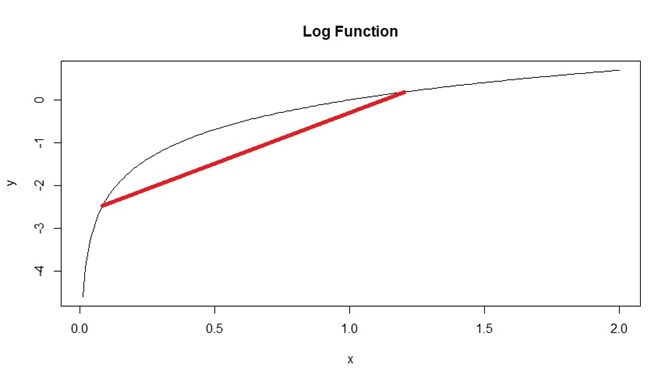
\includegraphics{images/06-concave.jpeg}
\caption{\label{fig:concave}Example of Concave Function}
\end{figure}

\begin{itemize}
\tightlist
\item
  \(g(x) = x^2\) is a convex function.

  \begin{itemize}
  \tightlist
  \item
    Its second derivative is \(g^{\prime \prime}(x) = 2\), which is always positive.
  \item
    We can also look at a graph of \(y = x^2\), and draw line segments that join two points on its graph. All of these lines are never below the graph. Figure \ref{fig:convex} below shows an example with one line segment, but we can see that any line segment that joins two points on the graph will never be below the graph.
  \end{itemize}
\end{itemize}

\begin{figure}
\centering
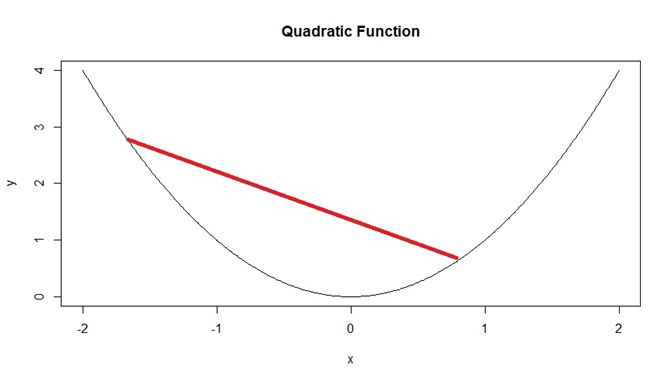
\includegraphics{images/06-convex.jpeg}
\caption{\label{fig:convex}Example of Convex Function}
\end{figure}

\emph{Thought question}: Consider the function \(g(x) = \frac{1}{x}\), i.e.~the inverse function. Can you explain why this function is convex when \(x>0\) and is concave when \(x<0\)?

\subsubsection{Jensen's Inequality}\label{jensens-inequality-1}

We are now ready to state \textbf{Jensen's inequality}. Let \(X\) denote a random variable. If \(g\) is convex, then \(E(g(X)) \geq g(E(X))\). If \(g\) is concave, then \(E(g(X)) \leq g(E(X))\).

The equality holds only if \(g\) is a linear function. It turns out linear functions are both convex and concave. The book goes through a simple proof of Jensen's inequality and is worth reading. Next, we apply Jensen's inequality to a few examples:

\begin{enumerate}
\def\labelenumi{\arabic{enumi}.}
\item
  We apply Jensen's inequality to the toy example in Section \ref{linnonlin}. As a reminder, suppose we roll a fair six-sided die, and let \(X\) denote the number of dots the die shows. The winnings is defined as the squared of the number of dots the die shows. Let \(T\) denote the new winnings, so \(T = X^2\), so \(g(x) = x^2\) is the function representing this non linear transformation. We established that the quadratic function is convex, so Jensen's inequality tells us that \(E(g(X)) \geq g(E(X))\), i.e.~that \(E(T) > E(X)^2\) which we showed in the code.
\item
  As mentioned in Section \ref{linnonlin}, a log transformation is often applied to make data that are right skewed less skewed, so that popular methods such as linear regression, tree based methods, \(K\) nearest neighbors can be used (these methods can be sensitive to outliers since they are based on conditional expectations or conditional means). What often happens is the log transformation is applied to the variable of interest, the model is fit, a prediction is made for the log transformed variable using conditional expectations, and the exponential is applied to this predicted value to convert it back to the original variable. Jensen's inequality tells us that the exponential of the average log variable is greater than the average variable, and our model over estimates.
\item
  Jensen's inequality can also be used to show that the sample standard deviation is a biased estimator of the population standard deviation, which appears counter intuitive, since the sample variance is an unbiased estimator of the population variance, i.e.~\(E(s^2) = \sigma^2\), but \(E(s) \neq \sigma\). The quick proof is
\end{enumerate}

\[
E(s) = E(\sqrt{s^2}) \leq \sqrt{E(s^2)} = \sigma.
\]

So the sample standard deviation underestimates the population standard deviation. However, this bias tends to be small if the sample size is large. We will cover ideas relating to unbiased estimators in a future module in more detail.

\subsection{Chebyshev's Inequality}\label{chebyshevs-inequality}

A common inequality that is used for probability is \textbf{Chebyshev's inequality}. It provides an upper bound on the probability that a random variable is at least a certain distance from its mean. Let \(X\) be a random variable with mean \(\mu\) and variance \(\sigma^2\). Then for any \(a>0\),

\begin{equation} 
P(|X-\mu| \geq a) \leq \frac{\sigma^2}{a^2}.
\label{eq:6-CI}
\end{equation}

An alternative way of expressing Chebyshev's inequality is to let \(a = c \sigma\) in equation \eqref{eq:6-CI}, so that it can be interpreted as providing an upper bound on the probability that a random variable is at least \(c\) standard deviations from its mean:

\begin{equation} 
P(|X-\mu| \geq c \sigma) \leq \frac{\sigma^2}{c^2 \sigma^2} = \frac{1}{c^2}.
\label{eq:6-CIalt}
\end{equation}

Using equation \eqref{eq:6-CIalt}, we can say the following about the upper bond on the probability that a random variable is at least 1, 2, and 3 standard deviations from its mean:

\begin{itemize}
\tightlist
\item
  When \(c=1\),
\end{itemize}

\[
P(|X-\mu| \geq \sigma) \leq \frac{1}{1^2} = 1.
\]
This informs us that the probability that a random variable is at least one standard deviation from its mean is no more than 1. The upper bound is not very informative in this setting since we know probabilities cannot be greater than 1.

\begin{itemize}
\tightlist
\item
  When \(c=2\),
\end{itemize}

\[
P(|X-\mu| \geq 2\sigma) \leq \frac{1}{2^2} = 0.25.
\]

This informs us the probability that a random variable is at least two standard deviations from its mean is no more than 0.25. In other words, there cannot be more than a 25\% chance that a random variable is at least 2 standard deviations from its mean, or there cannot be less than a 75\% chance that a random variable is within 2 standard deviations from its mean, since \(P(|X-\mu| \leq 2\sigma)\) is the complement of \(P(|X-\mu| \geq 2\sigma)\).

\begin{itemize}
\tightlist
\item
  When \(c=3\),
\end{itemize}

\[
P(|X-\mu| \geq 3\sigma) \leq \frac{1}{3^2} = \frac{1}{9}.
\]

There cannot be more than a 11.11\% chance that a random variable is at least 3 standard deviations from its mean, or there cannot be less than a 88.89\% chance that a random variable is within 3 standard deviations from its mean.

\emph{Thought question}: Can you explain how these results are consistent with the 68-99-99.7\% rule for normal distributions, as stated in Section \ref{rulenorm}?

Notice that Chebyshev's inequality can be applied to any distribution, and can be used to provide bounds on how data can be spread out. It is more flexible than the 68-99-99.7\% rule for normal distributions as it can be applied to any distribution, but the bounds are not as exact as they are an inequality. There can be a trade-off in relaxing assumptions and accuracy of results.

\section{Limit Theorems}\label{limits}

In the previous subsection, we used inequalities to provide bounds on probabilities and expectations that may be difficult to calculate. Another way of handing difficult calculations would be to use approximations for the distribution of the random variable, instead of the exact distribution of the random variable. Generally speaking, these approximations work better when we have more data (i.e.~when the sample size is larger). These approximations are covered by two of the most important limit theorems: the Law of Large Numbers and the Central Limit Theorem. These theorems approximate the distribution of the sample mean of i.i.d. (independent and identically distributed) random variables as the sample size gets larger.

Note: The idea of i.i.d. random variables implies that each observed value of the random variable is independent of each other, and that each observed value come from the same random variable. For example, let \(X\) denote the number of dots from a roll of a 6-sided fair die, and let \(X_1, X_2\) denote the value of the first and second roll respectively. \(X_1\) and \(X_2\) are i.i.d. since the outcomes from the first and second roll do not influence each other, so they are independent. \(X_1\) and \(X_2\) are identically distributed as they both follow the same distribution, \(Mult_6(1, (1/6, 1/6, 1/6, 1/6, 1/6, 1/6))\).

For the rest of this section, Section \ref{limits}, assume we have i.i.d. \(X_1, \cdots, X_n\) with finite mean \(\mu\) and finite variance \(\sigma^2\). For all positive integers \(n\) (i.e.~for any possible sample size), define the sample mean as \(\bar{X}_n = \frac{X_1 + \cdots + X_n}{n}\). We can easily derive the expected value and variance of the sample mean using properties of expectations and variances. Its expected value is

\begin{equation} 
\begin{split}
E(\bar{X}_n) &= E(\frac{X_1 + \cdots + X_n}{n}) \\
             &= \frac{1}{n}E(X_1 + \cdots + X_n) \\
             &= \frac{1}{n} (E(X_1) + \cdots + E(X_n)) \\
             &= \frac{1}{n} (\mu + \cdots + \mu) \\
             &= \mu.
\end{split}
\label{eq:6-Emean}
\end{equation}

Its variance is

\begin{equation} 
\begin{split}
Var(\bar{X}_n) &= Var(\frac{X_1 + \cdots + X_n}{n}) \\
             &= \frac{1}{n^2}Var(X_1 + \cdots + X_n) \\
             &= \frac{1}{n^2} (Var(X_1) + \cdots + Var(X_n)) \\
             &= \frac{1}{n^2} (\sigma^2 + \cdots + \sigma^2) \\
             &= \frac{\sigma^2}{n}.
\end{split}
\label{eq:6-Varmean}
\end{equation}

View the video below for a more detailed explanation of these results:

Equation \eqref{eq:6-Emean} informs us that the long-run average of sample means is equal to the population mean. We can imagine this if we had taken different random samples of size \(n\) from a population, and for each random sample we find the sample mean, and then average all these sample means. This average equals to the population mean \(\mu\). The code below provides a demonstration of these steps:

\begin{itemize}
\tightlist
\item
  We simulate a random sample of \(X_1, \cdots, X_{500}\) i.i.d. from standard normal.
\item
  Compute the sample mean and store it.
\item
  Repeat the previous steps for a total of 10 thousand reps.
\item
  Find the average of the 10 thousand sample means.
\end{itemize}

\begin{Shaded}
\begin{Highlighting}[]
\NormalTok{reps}\OtherTok{\textless{}{-}} \DecValTok{10000} \DocumentationTok{\#\#take 10000 random samples. This value should be large}
\NormalTok{n}\OtherTok{\textless{}{-}}\DecValTok{500} \DocumentationTok{\#\#sample size for each random sample}
\NormalTok{xbar}\OtherTok{\textless{}{-}}\FunctionTok{array}\NormalTok{(}\DecValTok{0}\NormalTok{,reps) }\DocumentationTok{\#\#store the sample mean for each random sample}

\FunctionTok{set.seed}\NormalTok{(}\DecValTok{90}\NormalTok{)}

\ControlFlowTok{for}\NormalTok{ (i }\ControlFlowTok{in} \DecValTok{1}\SpecialCharTok{:}\NormalTok{reps)}
  
\NormalTok{\{}
  
\NormalTok{  xbar[i]}\OtherTok{\textless{}{-}}\FunctionTok{mean}\NormalTok{(}\FunctionTok{rnorm}\NormalTok{(n)) }\DocumentationTok{\#\#find and store sample mean for each random sample}
  
\NormalTok{\}}

\FunctionTok{mean}\NormalTok{(xbar) }\DocumentationTok{\#\#average the sample means. This should be close to 0. }
\end{Highlighting}
\end{Shaded}

\begin{verbatim}
## [1] -0.0001034368
\end{verbatim}

Equation \eqref{eq:6-Varmean} informs us how to calculate the variance of the sample means. We can imagine this if we had taken different random samples of size \(n\) from a population, and for each random sample we find the sample mean, and then find the variance of all these sample means. It is the variance of the original random variable divided by \(n\). This means as the sample size gets larger, the variance of the sample means get smaller, in other words, the sample means tend to get closer to the population mean. We re run the code from above and also find the variance of the sample means.

\begin{Shaded}
\begin{Highlighting}[]
\FunctionTok{var}\NormalTok{(xbar) }\DocumentationTok{\#\#variance of sample means. This should be close to 1/500, since n=500. }
\end{Highlighting}
\end{Shaded}

\begin{verbatim}
## [1] 0.001979948
\end{verbatim}

\subsection{Law of Large Numbers}\label{law-of-large-numbers}

The \textbf{Law of Large Numbers (LLN)} states that as \(n\) gets larger and approaches infinity, the sample mean \(\bar{X}_n\) converges to the true mean \(\mu\). This implies that the sample mean tends to get closer to the population mean with larger sample sizes. The key word here is tends to, it is not a guarantee that the sample mean always gets closer to the population mean whenever \(n\) gets larger, but it generally does. This explains why we tend to trust results from larger sample sizes.

Another implication of the LLN is that we can use simulations to verify theoretical results, since these results usually require us to simulate data based on a large number of independent replications.

The LLN is a by product of equations \eqref{eq:6-Emean} and \eqref{eq:6-Varmean}. Equation \eqref{eq:6-Varmean} informs us that as \(n\) gets larger, the variance of the sample mean gets smaller. Equation \eqref{eq:6-Emean} informs us that the sample mean is unbiased, i.e.~its long run average is equal to the true mean. Collectively, these inform us that as \(n\) gets larger, the sample mean is more likely to be closer to the true mean.

We use an example to illustrate the LLN, which comes from flipping a fair coin. Let \(X\) denote whether the coin lands heads or tails, and let \(X=1\) for heads and \(X=0\) for tails. We can say that \(X \sim Bern(0.5)\) since the coin is fair. Imagine flipping the coin \(n\) times, and record the outcome after each flip, so \(X_1, \cdots, X_n\) denote the outcome of each flip. We know that \(E(X) = 0.5\) since \(X \sim Bern(0.5)\). The LLN informs us that \(\bar{X}_1, \cdots, \bar{X}_n\) should usually get closer to 0.5 as \(n\) increases. In other words, the value of the sample proportion after each flip should get usually closer to 0.5 with more flips. The code below simulates this example for \(n=500\), and Figure \ref{fig:4-LLN2} shows how the sample proportions get closer to 0.5, in general, as \(n\) increases.

\begin{Shaded}
\begin{Highlighting}[]
\NormalTok{n}\OtherTok{\textless{}{-}}\DecValTok{500} \DocumentationTok{\#\#make this big, but not too big otherwise picture is difficult to see}

\FunctionTok{set.seed}\NormalTok{(}\DecValTok{23}\NormalTok{)}

\NormalTok{X}\OtherTok{\textless{}{-}}\FunctionTok{rbinom}\NormalTok{(n,}\DecValTok{1}\NormalTok{,}\FloatTok{0.5}\NormalTok{) }\DocumentationTok{\#\#simulate 500 flips of fair coin}

\NormalTok{totals}\OtherTok{\textless{}{-}}\FunctionTok{cumsum}\NormalTok{(X) }\DocumentationTok{\#\#count total number of heads after each flip}
\NormalTok{index}\OtherTok{\textless{}{-}}\DecValTok{1}\SpecialCharTok{:}\NormalTok{n}
\NormalTok{props}\OtherTok{\textless{}{-}}\NormalTok{totals}\SpecialCharTok{/}\NormalTok{index }\DocumentationTok{\#\#find proportion of heads after each flip}

\DocumentationTok{\#\#create visual. LLN says that as n gets larger, the value of the sample proportion tends to get closer to 0.5}
\FunctionTok{plot}\NormalTok{(props, }\AttributeTok{type=}\StringTok{"l"}\NormalTok{, }\AttributeTok{main=}\StringTok{"Prop vs Sample Size"}\NormalTok{, }\AttributeTok{ylab=}\StringTok{"Proportion"}\NormalTok{, }\AttributeTok{xlab=}\StringTok{"n"}\NormalTok{)}
\FunctionTok{abline}\NormalTok{(}\AttributeTok{h=}\FloatTok{0.5}\NormalTok{, }\AttributeTok{col=}\StringTok{"blue"}\NormalTok{) }\DocumentationTok{\#\#overlay 0.5 for easy comparison}
\end{Highlighting}
\end{Shaded}

\begin{figure}
\centering
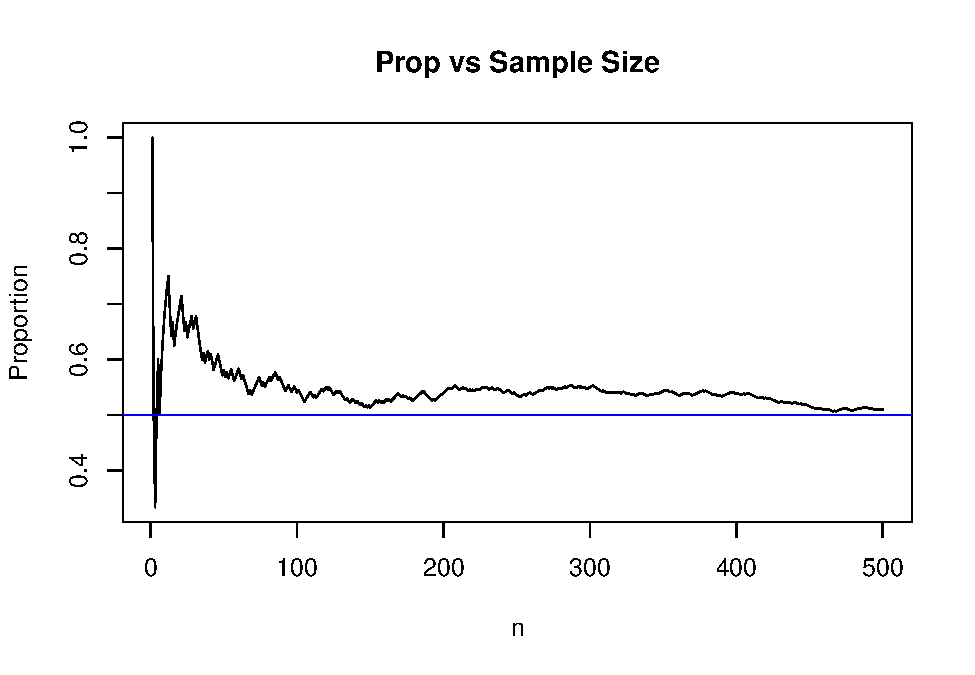
\includegraphics{bookdown-demo_files/figure-latex/4-LLN2-1.pdf}
\caption{\label{fig:4-LLN2}LLN Example 2}
\end{figure}

View the video below for a more detailed explanation of the code:

Note: \texttt{set.seed()} was used so you can reproduce these results exactly. However, the observation that the sample mean tends to get closer to the true mean as \(n\) increases will happen regardless of what \texttt{set.seed()} was used, or even if \texttt{set.seed()} was not used.

Note: The LLN actually comes in two versions, the Weak Law of Large Numbers (WLLN), and the Strong Law of Large Numbers (SLLN). The book goes into some detail about their definitions and differences. What I have written gives an intuitive explanation of what the LLN implies.

\subsubsection{Misconceptions with LLN}\label{misconceptions-with-lln}

One key idea with the LLN is that the sample mean \textbf{tends to get closer to the true mean as \(n\) gets larger}. The key words here are ``tends'' and ``as \(n\) gets larger''.

A misunderstanding of the LLN is the \textbf{gambler's fallacy}, which erroneously believes that the sample mean must ``self correct'' and get closer to the population mean with small increments of \(n\).

Using the example from flipping a fair coin. The gambler's fallacy erroneously thinks that:

\begin{itemize}
\tightlist
\item
  The proportion of heads should be close to 0.5, even with small \(n\).
\item
  The results of subsequent flips should self correct, i.e.~the proportion of heads get closer to 0.5 with the next flip. For example, if the first 5 flips are heads, the next flip is ``due'' to be tails since the proportion should get closer to 0.5 with the next flip.
\end{itemize}

The convergence to 0.5 comes from flipping the coin many times.

\subsection{Central Limit Theorem}\label{CLT}

The LLN informs us that the sample mean converges to the true mean. Statistical theory informs us about the expected value and variance of the sample mean in equations \eqref{eq:6-Emean} and \eqref{eq:6-Varmean}. But these do not inform us about the distribution of \(\bar{X}_n\). This is where the \textbf{Central Limit Theorem (CLT)} comes in.

The CLT states that as the sample size gets larger and tends to infinity, the distribution of \(\bar{X}_n\) after standardization approaches a standard normal distribution, i.e.

\begin{equation} 
\sqrt{n} \left(\frac{\bar{X}_n \ - \mu}{\sigma} \right) \to N(0,1).
\label{eq:6-CLT}
\end{equation}

The CLT is called an \textbf{asymptotic} result, as it informs us about the \textbf{limiting distribution} of \(\bar{X}_n\) as \(n\) gets larger and tends to infinity. The CLT implies an approximation when \(n\) is large enough. For large \(n\), the distribution of \(\bar{X}_n\) is approximately \(N(\mu, \frac{\sigma^2}{n})\).

The implication of the CLT is that even if our data do not follow a normal distribution, the average value of the data can be approximated by a normal distribution if our sample size is large enough. As mentioned in Section \ref{normdist}, a lot of questions in research deal with averages.

We consider this hypothetical situation. Suppose the waiting time for customers calling customer service during lunch time is known have a mean of 600 seconds with standard deviation 30 seconds. The company decides to cut costs and reduces staffing at the call center, and claims that wait times are not affected negatively. The customers are convinced otherwise. A researchers obtains the wait times from 500 customers who call in during lunch time after staffing is reduced. The sample mean of the wait times for these customers is 700 seconds. Can this data be used to counter the company's claim that wait times have been affected?

One possible calculation will be to assume the company is correct, that wait times have not changed, on average. If so, the sample means will be approximately normal, with mean 600 and variance \(\frac{30^2}{\sqrt{500}}\), i.e.~\(\bar{X}_{500} \sim N(600, \frac{30^2}{\sqrt{500}})\). We then calculate \(P(\bar{X}_{500} \geq 700)\), the probability that we have sample mean that is equal to or greater than 700 seconds. Using R, this probability is about 0.0065, which is very small, indicating that our data is inconsistent with the company's claim.

\begin{Shaded}
\begin{Highlighting}[]
\DecValTok{1}\SpecialCharTok{{-}}\FunctionTok{pnorm}\NormalTok{(}\DecValTok{700}\NormalTok{, }\DecValTok{600}\NormalTok{, }\DecValTok{30}\SpecialCharTok{\^{}}\DecValTok{2}\SpecialCharTok{/}\FunctionTok{sqrt}\NormalTok{(}\DecValTok{500}\NormalTok{))}
\end{Highlighting}
\end{Shaded}

\begin{verbatim}
## [1] 0.006486311
\end{verbatim}

The CLT is traditionally associated with the distribution of the sample mean \(\bar{X}_n\). It can be applied to the sum as well, due to properties of expectations and variances. Let \(T_n = X_1 + \cdots + X_n = n \bar{X}_n\) denote the sum of \(n\) i.i.d. random variables. The CLT says that, for large \(n\), the distribution of \(T_n\) is approximately \(N(n\mu, n\sigma^2)\).

\subsubsection{Considerations with CLT}\label{considerCLT}

One question that is raised when the CLT is used is how large does the sample size \(n\) have to be for the approximation to be accurate? While suggestions are plentiful (usually along the lines to sample size being at least 25 or 30), there is no fixed answer to this question. It depends on the distribution of \(X\). In general, the more skewed \(X\) is, \(n\) needs to be larger for the approximation to work. On the other hand, if \(X\) is already normal, then the distribution of \(\bar{X}_n\) is exactly \(N(\mu, \frac{\sigma^2}{n})\) for any sample size \(n\). We look at a couple of examples based on different distributions.

\begin{enumerate}
\def\labelenumi{\arabic{enumi}.}
\tightlist
\item
  \(X\) is standard normal. Our code will do the following:
\end{enumerate}

\begin{itemize}
\tightlist
\item
  We simulate \(n\) draws from \(X\) for \(n = 1\).
\item
  To obtain the distribution of \(\bar{X}_n\) for each value of \(n\), we repeat the previous step for a total of 10 thousand reps, then produce a histogram of the 10 thousand values of \(\bar{X}_n\).
\item
  Repeat the previous two steps, with different values of \(n\). We will use \(n= 5, 30, 100\) as well
\item
  We expect the histograms for \(\bar{X}_n\) to all look normal for all values of \(n\) we used.
\end{itemize}

\begin{figure}
\centering
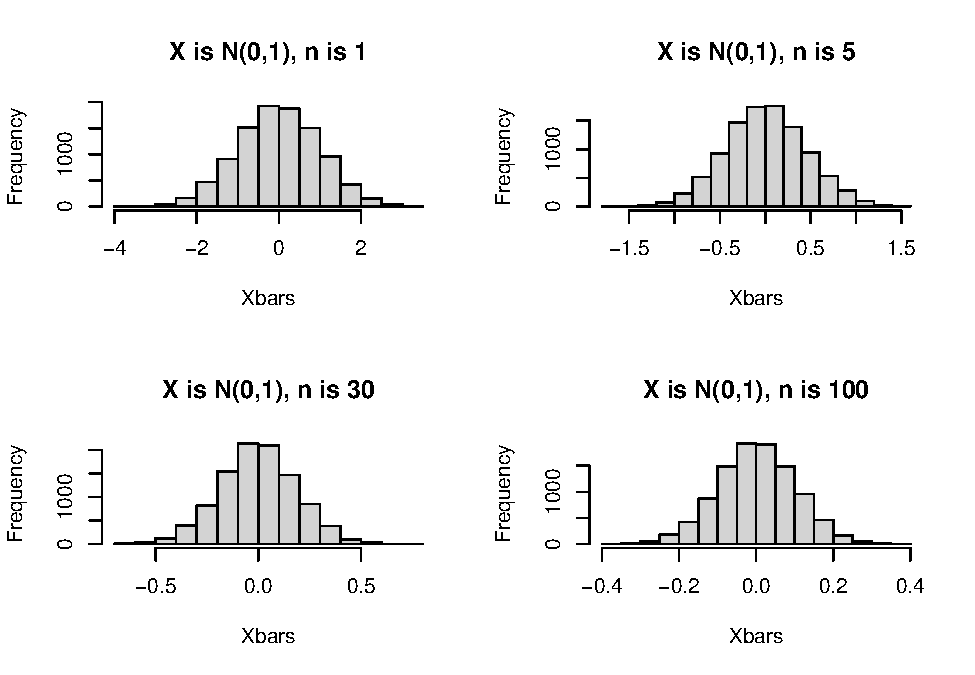
\includegraphics{bookdown-demo_files/figure-latex/6-CLTnorm-1.pdf}
\caption{\label{fig:6-CLTnorm}Distribution of Sample Means when X is N(0,1), n varied}
\end{figure}

Figure \ref{fig:6-CLTnorm} displays the histograms from this simulation, and matches what we expect from the CLT. Since \(X\) is normal, \(\bar{X}_n\) follows a normal distribution for any value of \(n\).

\begin{enumerate}
\def\labelenumi{\arabic{enumi}.}
\setcounter{enumi}{1}
\tightlist
\item
  \(X\) is Poisson with parameter 1. This is a skewed distribution. We use code that mimics the previous example, with the only difference being that our data are simulated from \(Pois(1)\) instead of standard normal. When \(n\) is small, we expect the distribution of \(\bar{X}_n\) to not look normal. As \(n\) gets larger, we expect the distribution of \(\bar{X}_n\) will look more normal.
\end{enumerate}

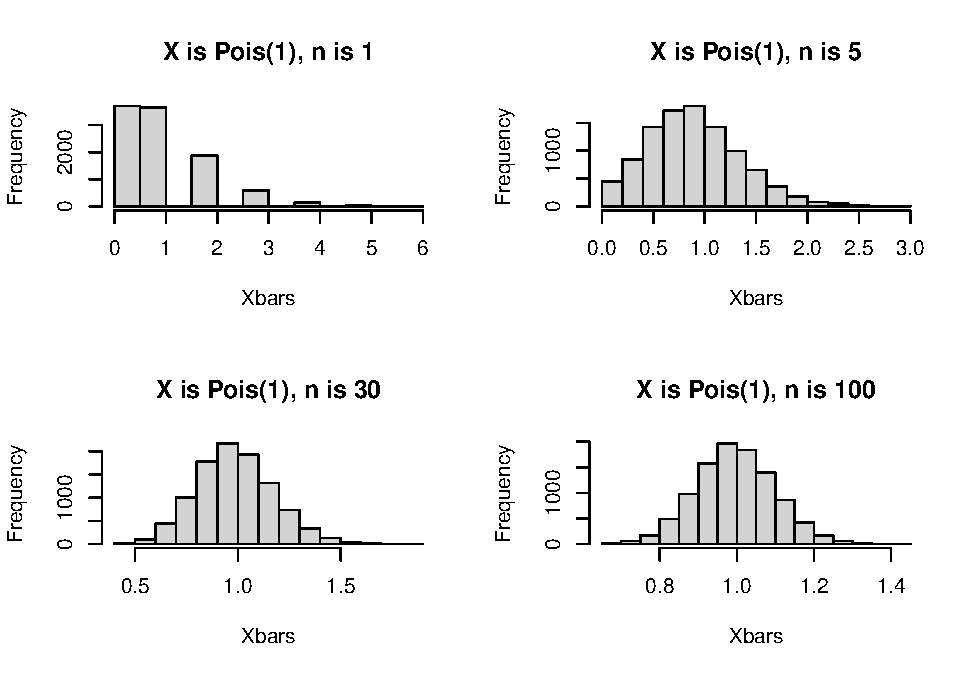
\includegraphics{bookdown-demo_files/figure-latex/6-CLTpois-1.pdf}
Figure \ref{fig:6-CLTpois} displays the histograms from this simulation, and matches what we expect. When \(n\) is 1 or 5, the histograms are clearly not normal, so the CLT approximation will not work well. When \(n=30\) the histogram looks approximately normal, and when \(n=100\), the histogram looks even closer to a normal distribution.

\section{Monte Carlo Simulations}\label{monte-carlo-simulations}

You may have noticed that we have used simulations in the earlier sections of this module (and previous modules) to help explain certain concepts. These simulations are called \textbf{Monte Carlo} methods, or Monte Carlo simulations. The idea behind Monte Carlo methods is to used repeated random sampling (and by repeated, we mean repeated a large number of times) to estimate features of data, usually probabilities and expected values. Monte Carlo methods are used for the following purposes:

\begin{enumerate}
\def\labelenumi{\arabic{enumi}.}
\item
  When the probability or expectation is too complicated to work out by hand. Recall that finding probabilities and expectations by hand involve summations or integrals, and it becomes obvious that working with summations and especially integrals can get onerous.
\item
  To verify theoretical results involving probability or expectations. While a lot of theory is proved using mathematics, most academic papers include Monte Carlo simulations to verify the theoretical results. We have done these to verify the LLN and CLT in the previous subsection (under some circumstances).
\item
  To help confirm that you understand the meaning of theoretical results. The only way your code matches the theory is if you understand the theory.
\end{enumerate}

\subsection{Monte Carlo Methods for Expected Values}\label{monte-carlo-methods-for-expected-values}

Suppose we want to find some expectation for a continuous random variable \(X\), \(E(g(X))\), where \(g\) is some function. LOTUS says that we need to use equation \eqref{eq:4-lotus}, i.e.~\(E(g(X)) = \int_{-\infty}^{\infty} g(x) f_X(x).\) Monte Carlo methods avoid doing this integration by simulating \(X_1, \cdots, X_M\) from \(X\) and estimate \(E(g(X))\) with the sample mean of \(g(X)\), \(\frac{1}{M} \sum_{i=1}^M g(X_i)\). The LLN tells us that as \(M\) gets larger, this sample mean converges to \(E(g(X))\).

Monte Carlo methods replace the integral (or summation) with simulating a random variable repeatedly many times. We use a simple example to illustrate this idea.

Let \(X\) be a standard normal distribution. Suppose we want to find the value of \(E(X^2)\). If we try to find this using LOTUS, we will need to find \(\int_{-\infty}^{\infty} x^2 \frac{1}{\sqrt{2 \pi}} e^{-x^2/2} dx\). Instead of working out this integral by hand, we carry out a Monte Carlo simulation by doing these steps:

\begin{itemize}
\tightlist
\item
  Simulate \(M\) random values from a standard normal, where \(M\) is large.
\item
  Calculate \(X_1^2, \cdots, X_M^2\).
\item
  Find the sample average of \(X_1^2, \cdots, X_M^2\).
\end{itemize}

\begin{Shaded}
\begin{Highlighting}[]
\FunctionTok{set.seed}\NormalTok{(}\DecValTok{5}\NormalTok{)}

\NormalTok{reps}\OtherTok{\textless{}{-}}\DecValTok{10000} \DocumentationTok{\#\# this is M}

\NormalTok{Xs}\OtherTok{\textless{}{-}}\FunctionTok{rnorm}\NormalTok{(reps) }\DocumentationTok{\#\#generate M values of X}

\NormalTok{squared.values}\OtherTok{\textless{}{-}}\NormalTok{Xs}\SpecialCharTok{\^{}}\DecValTok{2} \DocumentationTok{\#\#square each X}

\FunctionTok{mean}\NormalTok{(squared.values) }\DocumentationTok{\#\#sample average of squared values. }
\end{Highlighting}
\end{Shaded}

\begin{verbatim}
## [1] 1.024546
\end{verbatim}

\begin{Shaded}
\begin{Highlighting}[]
\DocumentationTok{\#\#when reps is large, this sample mean should be close to the true E(X\^{}2), which is 1}
\end{Highlighting}
\end{Shaded}

Since \(X\) is standard normal, we know \(E(X) = 0\) and \(Var(X) = E(X^2) - E(X)^2 = E(X^2) = 1\). We see in our simulation that our estimated value for \(E(X^2)\) is pretty close to its theoretical value.

\subsection{Monte Carlo Methods for Probabilities}\label{monte-carlo-methods-for-probabilities}

Suppose we want to find the probability that a random variable satisfies some event \(E\), \(P(E)\). We could perform a summation or integral to find this probability, or estimate the probability using Monte Carlo methods. What we will do is simulate \(X_1, \cdots, X_M\) from \(X\), where \(M\) is large, in other words, simulate a large number of replicates of \(X\). We then count how many of the \(X_i\)s correspond to event \(E\) happening, and then divide this number by \(M\), the number of replicates. We use an example to illustrate this idea.

Let \(X\) be a standard normal distribution. Suppose we want to find the probability \(P(X^2 > 1)\). We carry out a Monte Carlo simulation by doing these steps:

\begin{itemize}
\tightlist
\item
  Simulate \(M\) random values from a standard normal, where \(M\) is large.
\item
  Calculate \(X_1^2, \cdots, X_M^2\).
\item
  Count the number of times \(X_i^2\) is greater than 1.
\item
  Divide this number by \(M\) to estimate the probability, since probability can be interpreted as a long-run proportion.
\end{itemize}

\begin{Shaded}
\begin{Highlighting}[]
\FunctionTok{set.seed}\NormalTok{(}\DecValTok{5}\NormalTok{)}

\NormalTok{reps}\OtherTok{\textless{}{-}}\DecValTok{10000} \DocumentationTok{\#\# this is M}

\NormalTok{Xs}\OtherTok{\textless{}{-}}\FunctionTok{rnorm}\NormalTok{(reps) }\DocumentationTok{\#\#generate M values of X}

\NormalTok{squared.values}\OtherTok{\textless{}{-}}\NormalTok{Xs}\SpecialCharTok{\^{}}\DecValTok{2} \DocumentationTok{\#\#square each X}

\FunctionTok{sum}\NormalTok{(squared.values}\SpecialCharTok{\textgreater{}}\DecValTok{1}\NormalTok{)}\SpecialCharTok{/}\NormalTok{reps }\DocumentationTok{\#\#count the number of times X\^{}2 is greater than 1, and divide by M}
\end{Highlighting}
\end{Shaded}

\begin{verbatim}
## [1] 0.3178
\end{verbatim}

\begin{Shaded}
\begin{Highlighting}[]
\DocumentationTok{\#\#when reps is large, this proportion should be close to}
\DecValTok{1}\SpecialCharTok{{-}}\FunctionTok{pchisq}\NormalTok{(}\DecValTok{1}\NormalTok{, }\AttributeTok{df=}\DecValTok{1}\NormalTok{)}
\end{Highlighting}
\end{Shaded}

\begin{verbatim}
## [1] 0.3173105
\end{verbatim}

\begin{Shaded}
\begin{Highlighting}[]
\DocumentationTok{\#\#it turns out that squaring a standard normal gives a chi{-}squared distribution with 1 df.}
\end{Highlighting}
\end{Shaded}

We see the estimated probability \(P(X^2 > 1)\) is close to its theoretical probability.

\subsection{Monte Carlo Methods for Other Purposes}\label{monte-carlo-methods-for-other-purposes}

Monte Carlo methods are not exclusively used estimating expected values and probabilities. They are versatile and can be used for a number of purposes, as long we need repeated random sampling.

A fun example that is pretty famous uses Monte Carlo simulations to estimate the value of \(\pi\). We can consider the following hypothetical dart throwing experiment to do so, based on the figure below:

\begin{figure}
\centering
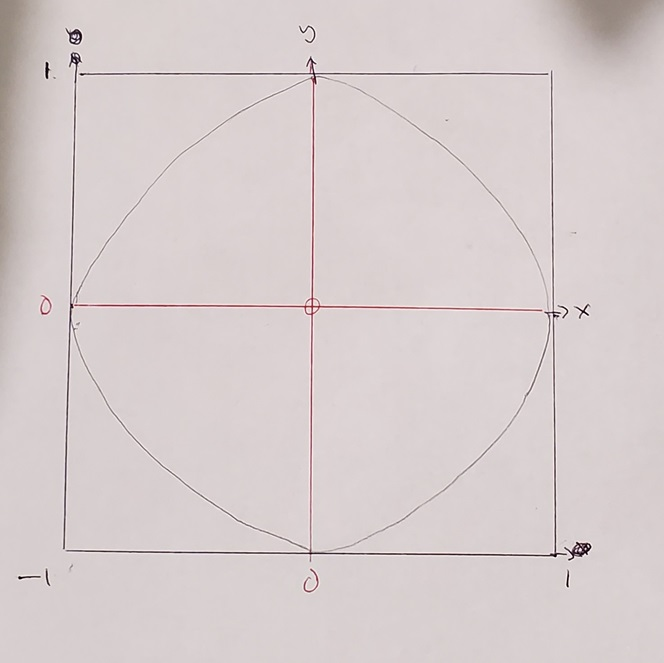
\includegraphics{images/06-circle.jpg}
\caption{\label{fig:circle}Board for Dart Throwing Experiment}
\end{figure}

The experiment works in this way:

\begin{itemize}
\tightlist
\item
  The dart will always land in the square, and has an equal probability of landing on any spot on the square.

  \begin{itemize}
  \tightlist
  \item
    We can let \(X \sim U(-1,1)\) to represent the position of the dart on the x-axis of the circle in Figure \ref{fig:circle}.
  \item
    We can let \(Y \sim U(-1,1)\) to represent the position of the dart on the y-axis of the circle in Figure \ref{fig:circle}.
  \end{itemize}
\item
  We will throw a large number of darts. For each dart, we will see if it lands in the circle or not.

  \begin{itemize}
  \tightlist
  \item
    To assess if a dart lies in the circle, we assess whether \(x_i^2 + y_i^2 \leq 1\) for dart \(i\). If this condition is met, we know dart \(i\) lies in the circle, if not, it lies outside the circle.
  \end{itemize}
\item
  It stands to reason that \(\frac{\text{Area of circle}}{\text{Are of square}} = \frac{\pi}{4} \approx \frac{\text{Number of darts landing in circle}}{\text{Number of darts thrown}}\).
\item
  Therefore, after throwing a large number of darts, \(\pi \approx 4 \times \frac{\text{Number of darts landing in circle}}{\text{Number of darts thrown}}.\)
\end{itemize}

The code below carries out this experiment with 10 thousand reps (or 10 thousand dart throws):

\begin{Shaded}
\begin{Highlighting}[]
\NormalTok{reps}\OtherTok{\textless{}{-}}\DecValTok{10000} \DocumentationTok{\#\#number of dart throws}

\NormalTok{count}\OtherTok{\textless{}{-}}\DecValTok{0} \DocumentationTok{\#\#counter that keeps track of number of throws inside circle}

\FunctionTok{set.seed}\NormalTok{(}\DecValTok{222}\NormalTok{)}

\ControlFlowTok{for}\NormalTok{ (i }\ControlFlowTok{in} \DecValTok{1}\SpecialCharTok{:}\NormalTok{reps) \{}

\NormalTok{x}\OtherTok{\textless{}{-}}\FunctionTok{runif}\NormalTok{(}\DecValTok{1}\NormalTok{,}\AttributeTok{min=}\SpecialCharTok{{-}}\DecValTok{1}\NormalTok{, }\AttributeTok{max=}\DecValTok{1}\NormalTok{) }\DocumentationTok{\#\#simulate landing spot on x axis}
\NormalTok{y}\OtherTok{\textless{}{-}}\FunctionTok{runif}\NormalTok{(}\DecValTok{1}\NormalTok{,}\AttributeTok{min=}\SpecialCharTok{{-}}\DecValTok{1}\NormalTok{, }\AttributeTok{max=}\DecValTok{1}\NormalTok{) }\DocumentationTok{\#\#simulate landing spot on y axis}

  \ControlFlowTok{if}\NormalTok{ (x}\SpecialCharTok{\^{}}\DecValTok{2} \SpecialCharTok{+}\NormalTok{ y}\SpecialCharTok{\^{}}\DecValTok{2} \SpecialCharTok{\textless{}=} \DecValTok{1}\NormalTok{)\{}
\NormalTok{    count }\OtherTok{\textless{}{-}}\NormalTok{ count}\SpecialCharTok{+}\DecValTok{1} \DocumentationTok{\#\#counter adds 1 if dart lands in circle}
\NormalTok{  \}}

\NormalTok{\}}

\DocumentationTok{\#\#estimate pi. should be close to real value of pi. Gets closer if we throw more darts}
\NormalTok{count}\SpecialCharTok{/}\NormalTok{reps }\SpecialCharTok{*} \DecValTok{4} 
\end{Highlighting}
\end{Shaded}

\begin{verbatim}
## [1] 3.1436
\end{verbatim}

We see the estimated value for \(\pi\) using this Monte Carlo simulation is close to its true value.

\subsection{Considerations with Monte Carlo Methods}\label{considerations-with-monte-carlo-methods}

In the examples above, we compared estimated values using Monte Carlo methods with their real values, so we could see the methods work. However, if we do not know the real values, two questions will come to mind:

\begin{enumerate}
\def\labelenumi{\arabic{enumi}.}
\item
  How many replicates do we need? We only know the estimated values converge to the true values as we increase the number of replicates. Using more replicates will make the simulation run longer on your computer.
\item
  Related to the previous question, how close is close enough? How do you know your estimated value from the simulation is close enough to the truth? There is no way of knowing if the true value is unknown.
\end{enumerate}

\subsubsection{set.seed() in R}\label{set.seed-in-r}

You may have noticed that in the provided simulations, we use a function \texttt{set.seed()} and input a number. This is to enable others to replicate the exact same results, if someone wants to verify the code.

With Monte Carlo simulations, we are generating numbers randomly. When we set the seed with \texttt{set.seed()} with a certain number, we ensure the same random numbers are generated each time the code is run.

We will not go into the details of how R generates the random numbers, and random number generation is a whole field in itself.

In terms of running the examples, you can choose to copy the code and exclude the line with \texttt{set.seed()}. You should still observe that the estimated values from the simulations are close to the true values.

\chapter{Estimation}\label{est}

This module is based on Introduction to Probability for Data Science (Chan), Chapter 8.1 and 8.2. You can access the book for free at \url{https://probability4datascience.com}. Please note that I cover additional topics, and skip certain topics from the book. You may skip Section 8.1.3, 8.1.4, and 8.1.6 from the book.

\section{Introduction}\label{introduction-3}

We consider building models based on the data we have. Many models are based on some distribution, for example, the linear regression model is based on the normal distribution, and the logistic regression model is based on the Bernoulli distribution. Recall that these distributions are specified by their parameters: the mean \(\mu\) and variance \(\sigma^2\) for the normal distribution, and the success probability \(p\) for a Bernoulli distribution. The value of the parameters are almost always unknown in real life. This module deals with estimation: how we estimate the values of these parameters, as well as quantify the level of uncertainty we have with these estimated values, given the data we have.

\subsection{Big Picture Idea with Estimation}\label{big-picture-idea-with-estimation}

Consider this simple scenario. We want to find the distribution associated with the systolic blood pressure of American adults. To be able to achieve this goal, we would have to get the systolic blood pressure of every single American adult. This is usually not feasible as researchers are unlikely to have the time and money to interview every single American adult. Instead, a representative sample of American adults will be obtained, for example, 750 randomly selected American adults are interviewed. We can then create density plots, histograms, compute the mean, median, variance, skewness, and other summaries that may be of interest, based on these 750 American adults.

\subsubsection{Population Vs Sample}\label{population-vs-sample}

The above scenario illustrates a few concepts and terms that are fundamental in estimation. In any study, we must be clear as to who or what is the population of interest, and who or what is the sample.

The \textbf{population} (sometimes called the population of interest) is the entire set of individuals, or objects, or events that a study is interested in. In the scenario described above, the population would be (all) American adults.

The \textbf{sample} is the set of individuals, or objects, or events which we have data on. In the scenario described above, the sample is the 750 randomly selected American adults.

Ideally, the sample should be \textbf{representative} of the population. A representative sample is often achieved through a simple random sample, where each unit in the population has the same chance of being selected to be in the sample. In this module, we will assume that we have a representative sample. Note: You may feel that obtaining a simple random sample may be difficult. We will not get into a discussion of sampling (sometimes called survey sampling), which is a field of statistics that handles how to obtain representative samples, or how calculations should be adjusted if the sample is not representative. There is still a lot of research that is being done in survey sampling.

\subsubsection{Variables \& Observations}\label{variables-observations}

A \textbf{variable} is a characteristic or attribute of individuals, or objects, or events that make up the population and sample. In the above scenario, a variable would be the systolic blood pressure of American adults. We can use the notation of random variables to describe variables. For example, we can let \(X\) denote the systolic blood pressure of an American adult, so writing \(P(X>200)\) means we want to find the probability that an American adult has systolic blood pressure greater than 200 mm Hg .

An \textbf{observation} is the individual person, object or event that we collect data from. In the above scenario, an observation is a single American adult in our sample of 750.

One way to think about variables and observations is through a spreadsheet. Typically, each row represents an observation and each column represents a variable. Figure \ref{fig:07-dataframe} below displays such an example, based on the described scenario. Each row represents an observation, i.e.~a single American adult in our sample, and the column represents the variable, which is systolic blood pressure.

\begin{figure}
\centering
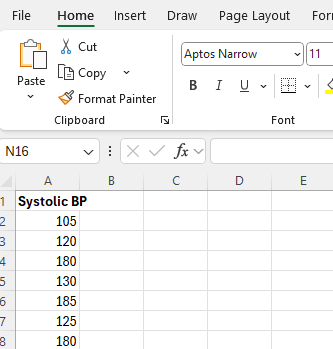
\includegraphics{images/07-dataframe.png}
\caption{\label{fig:07-dataframe}Example of Data in a Spreadsheet}
\end{figure}

\subsubsection{Parameter Vs Estimator}\label{parameter-vs-estimator}

Now that we have made the distinction between a population and a sample, we are ready to define parameters and estimators.

A \textbf{parameter} is a numerical summary associated with a population. In the scenario described above, an example of a population parameter would be the population mean systolic blood pressure of American adults.

An \textbf{estimator} is a numerical summary associated with samples. An estimator is typically used to estimate a parameter. In the scenario described above, an estimator of the population mean systolic blood pressure of American adults could be the average systolic blood pressure in our sample. So the sample mean is an estimator of the population mean.

An \textbf{estimated value}, or \textbf{estimate}, is the actual value of the estimator based on a sample. In the scenario described above, suppose the average systolic blood pressure of the 750 American adults is 140 mm Hg. We will say the estimated value of the mean systolic blood pressure of American adults is 140 mm Hg.

So a parameter is a number that is associated with a population, while an estimator is a number that is associated with a sample. Some other differences between parameters and estimators:

\begin{itemize}
\tightlist
\item
  The value of parameters are unknown, while we can actually calculate numerical values of estimators.
\item
  The value of parameters are considered fixed (as there is only one population), while the numerical values of estimators can vary if we obtain multiple random samples of the same sample size. Using the scenario above again, suppose we obtain a second representative sample of 750 American adults. The average systolic blood pressure of this second sample is likely to be different from the average systolic blood pressure of the first sample. This illustrates that there is \textbf{variance, or uncertainty, associated with estimators due to random sampling}. This is the uncertainty that we will be focusing on in this section.
\end{itemize}

Whenever we propose an estimator for a parameter, we want to assess how ``good'' the estimator is. In some situations, there is an obvious choice for an estimator, for example, using the sample mean, \(\bar{x} = \frac{\sum x_i}{n}\) to estimate the population mean. But in some instances, the choice may not be so obvious. For example, why do use the sample variance \(s^2 = \frac{\sum (x_i - \bar{x})^2}{n-1}\) as an estimator for the population variance, and not \(\frac{\sum (x_i - \bar{x})^2}{n}\)? We will cover a few measures that are used to assess an estimator: bias, variance, and mean-squared error.

We will also cover a couple of methods in estimating parameters: the method of moments, and the method of maximum likelihood. You will notice that we use probability rules in these methods.

To sum up estimation: we use data from a sample to estimate unknown characteristics of a population, so that we can answer questions regarding variables in the population, as well as provide a measure of uncertainty for our answers.

\section{Method of Moments Estimation}\label{MOM}

We will cover a couple of methods in estimation. The first method is the \textbf{method of moments}. It is a more intuitive method, although it lacks certain ideal properties. Before defining this method, we recall and define some terms.

In Section \ref{moments}, we defined \textbf{moments}. As a reminder, for a random variable \(X\), its \(k\)th moment is \(E(X^k)\), which can be found using LOTUS: \(\int_{-\infty}^{\infty} x^k f_X(x) dx\).

Suppose we observe a random sample \(x_1, \cdots, x_n\) that comes from \(X\). The \(k\)th \textbf{sample moment} is \(M_k = \frac{1}{n} \sum_{i=1}^n x_i^k\).

Using these definitions,

\begin{itemize}
\tightlist
\item
  The 1st moment is \(E(X) = \mu_x\), the population mean of \(X\).
\item
  The 1st sample moment is \(M_1 = \frac{1}{n} \sum_{i=1}^n x_i = \bar{x}\), the sample mean.
\item
  The 2nd moment is \(E(X^2)\).
\item
  The 2nd sample moment is \(M_2 = \frac{1}{n} \sum_{i=1}^n x_i^2\).
\end{itemize}

And so on.

The method of moments estimation is: Let \(X\) be a random variable with distribution depending on parameters \(\theta_1, \cdots, \theta_m\). The \textbf{method of moments (MOM) estimates} \(\hat{\theta}_1, \cdots, \hat{\theta}_m\) are found by equating the first \(m\) sample moments to the corresponding first \(m\) moments and solving for \(\theta_1, \cdots, \theta_m\).

You might have noticed that the method of moments is based on the Law of Large Numbers.

Note: By convention, parameters are typically denoted by Greek letters, and their estimators are denoted with a hat symbol over the corresponding letter.

Let us look at a couple of examples:

\begin{enumerate}
\def\labelenumi{\arabic{enumi}.}
\tightlist
\item
  Suppose I have a coin and I do not know if it is fair or not. There are only two outcomes on a flip, heads or tails. Each flip is independent of other flips. Let \(X_i\) denote whether the \(i\)th flip lands heads, where \(X_i = 1\) if heads and \(X_i = 0\) if tails. We can see that \(X_i \sim Bern(p)\), where \(p\) is the probability it lands heads. Derive the MOM estimate for \(p\).
\end{enumerate}

A Bernoulli distribution has only 1 parameter, \(p\), so when using the method of moments, we only need to equate the first sample moment to the first moment.

\begin{itemize}
\tightlist
\item
  The first moment is \(E(X_i) = p\), since \(X_i \sim Bern(p)\).
\item
  The first sample moment is \(M_1 = \frac{1}{n} \sum_{i=1}^n x_i = \bar{x}\).
\end{itemize}

Set \(E(X_i) = M_1\), i.e.~\(\hat{p} = \bar{x}\). Since \(X_i = 1\) if heads and \(X_i = 0\) if tails, \(\frac{1}{n} \sum_{i=1}^n x_i = \bar{x}\) actually represents the proportion of flips that land on heads, based on \(n\) flips. So this is actually the sample proportion.

The MOM estimate for this problem is \(\hat{p}\), the proportion of \(n\) flips that land on heads. This result should be fairly intuitive. If we flip a coin a large number of times, and 70\% of the flips land on heads, the sample proportion is \(\hat{p} = 0.7\), and so the estimated value for \(p\), the success probability is 0.7.

\begin{enumerate}
\def\labelenumi{\arabic{enumi}.}
\setcounter{enumi}{1}
\tightlist
\item
  Birth weights of newborn babies typically follow a normal distribution. We have data from births at Baystate Medical Center in Springfield, MA, during 1986. Assuming that the births at this hospital is representative of births in New England in 1986, derive the MOM estimates for \(\mu\) and \(\sigma^2\), the mean and variance of the distribution of birth weights in New England in 1986.
\end{enumerate}

A normal distribution has 2 parameters, \(\mu\) and \(\sigma^2\), so we need to equate the first two sample moments to the first two moments. Let \(X\) denote the birth weights in New England in 1986, so \(X \sim N(\mu, \sigma^2)\).

\begin{itemize}
\tightlist
\item
  The first moment is \(E(X) = \mu\), since \(X \sim N(\mu, \sigma^2)\).
\item
  The first sample moment is \(M_1 = \frac{1}{n} \sum_{i=1}^n x_i = \bar{x}\).
\end{itemize}

So we set \(E(X) = M_1\), i.e.~\(\hat{\mu} = \bar{x}\). This is just the sample average of the birth weights at Baystate Medical Center in 1986.

\begin{itemize}
\tightlist
\item
  The second moment is \(E(X^2)\). But we know that since \(X \sim N(\mu, \sigma^2)\).
\end{itemize}

\[
\begin{split}
Var(X) &= E(X^2) - E(X)^2\\
\implies E(X^2) &= Var(X) + E(X)^2 \\
\implies E(X^2) &= \sigma^2 + \mu^2
\end{split}
\]

\begin{itemize}
\tightlist
\item
  The second sample moment is \(M_2 = \frac{1}{n} \sum_{i=1}^n x_i^2\).
\end{itemize}

So we set \(E(X^2) = M_2\), i.e.~\(\hat{\sigma^2} + \hat{\mu}^2 = \frac{1}{n} \sum_{i=1}^n x_i^2\). Since we earlier found that \(\hat{\mu} = \bar{x}\), we get \(\hat{\sigma^2}  = \frac{1}{n} \sum_{i=1}^n x_i^2 - \bar{x}^2 = \frac{1}{n} \sum_{i=1}^n (x_i - \bar{x})^2\).

Therefore, the MOM estimates for \(\mu\) and \(\sigma^2\) are \(\hat{\mu} = \bar{x}\) and \(\hat{\sigma^2}  = \frac{1}{n} \sum_{i=1}^n (x_i - \bar{x})^2\) respectively.

View the video below for a more detailed explanation on deriving the MOM estimates for the normal distribution below:

We now use these MOM estimates on the data set of birth weights at Baystate Medical Center in 1986. It is well established in the literature that birth weights of babies follow a normal distribution. A quick check with the Shapiro-Wilk test for normality shows no contradiction, so we proceed with finding the estimates for \(\mu\) and \(\sigma^2\). We then produce a density plot of the birth weights, and overlay a curve that corresponds to a normal distribution with \(\hat{\mu} = \bar{x}\) and \(\hat{\sigma^2}  = \frac{1}{n} \sum_{i=1}^n (x_i - \bar{x})^2\). This normal curve is pretty close to the density plot, so it appears reasonable to say that the birth weights follow a normal distribution with mean 2944.587 (grams) and variance 528940 (grams-squared).

\begin{Shaded}
\begin{Highlighting}[]
\FunctionTok{library}\NormalTok{(MASS)}
\NormalTok{data}\OtherTok{\textless{}{-}}\NormalTok{MASS}\SpecialCharTok{::}\NormalTok{birthwt }\DocumentationTok{\#\#dataset comes from MASS package}

\FunctionTok{shapiro.test}\NormalTok{(data}\SpecialCharTok{$}\NormalTok{bwt) }\DocumentationTok{\#\#check for normality}
\end{Highlighting}
\end{Shaded}

\begin{verbatim}
## 
##  Shapiro-Wilk normality test
## 
## data:  data$bwt
## W = 0.99244, p-value = 0.4353
\end{verbatim}

\begin{Shaded}
\begin{Highlighting}[]
\NormalTok{mu}\OtherTok{\textless{}{-}}\FunctionTok{mean}\NormalTok{(data}\SpecialCharTok{$}\NormalTok{bwt) }\DocumentationTok{\#\#MOM estimate for mu}
\NormalTok{mu}
\end{Highlighting}
\end{Shaded}

\begin{verbatim}
## [1] 2944.587
\end{verbatim}

\begin{Shaded}
\begin{Highlighting}[]
\NormalTok{sigma2}\OtherTok{\textless{}{-}}\FunctionTok{mean}\NormalTok{((data}\SpecialCharTok{$}\NormalTok{bwt}\SpecialCharTok{{-}}\NormalTok{mu)}\SpecialCharTok{\^{}}\DecValTok{2}\NormalTok{) }\DocumentationTok{\#\#MOM estimate for sigma2}
\NormalTok{sigma2}
\end{Highlighting}
\end{Shaded}

\begin{verbatim}
## [1] 528940
\end{verbatim}

\begin{Shaded}
\begin{Highlighting}[]
\DocumentationTok{\#\#create density plot for data, and overlay Normal curve with parameters estimated by MOM}
\FunctionTok{plot}\NormalTok{(}\FunctionTok{density}\NormalTok{(data}\SpecialCharTok{$}\NormalTok{bwt), }\AttributeTok{main=}\StringTok{""}\NormalTok{, }\AttributeTok{ylim=}\FunctionTok{c}\NormalTok{(}\DecValTok{0}\NormalTok{,}\FloatTok{6e{-}04}\NormalTok{))}
\FunctionTok{curve}\NormalTok{(}\FunctionTok{dnorm}\NormalTok{(x, }\AttributeTok{mean=}\NormalTok{mu, }\AttributeTok{sd=}\FunctionTok{sqrt}\NormalTok{(sigma2)), }
      \AttributeTok{col=}\StringTok{"blue"}\NormalTok{, }\AttributeTok{lwd=}\DecValTok{2}\NormalTok{, }\AttributeTok{add=}\ConstantTok{TRUE}\NormalTok{)}
\end{Highlighting}
\end{Shaded}

\begin{figure}
\centering
\includegraphics{bookdown-demo_files/figure-latex/7-MOM-1.pdf}
\caption{\label{fig:7-MOM}Density Plot of Birth Weights. Normal Curve (in Blue) with Parameters Estimated by MOM Overlaid}
\end{figure}

\subsection{Alternative Form of Method of Moments Estimation}\label{alternative-form-of-method-of-moments-estimation}

In Section \ref{moments}, we defined \textbf{central moments}. As a reminder, for a random variable \(X\), its \(k\)th central moment is \(E((X-\mu)^k)\).

Suppose we observe a random sample \(x_1, \cdots, x_n\) that comes from \(X\). The \(k\)th \textbf{sample central moment} is \(M_k^* = \frac{1}{n} \sum_{i=1}^n (x_i - \bar{x})^k\).

An alternative form for the method of moments estimation is: Let \(X\) be a random variable with distribution depending on parameters \(\theta_1, \cdots, \theta_m\). The method of moments (MOM) estimates \(\hat{\theta}_1, \cdots, \hat{\theta}_m\) are found by equating the first sample moment to the first moments, and equating subsequent sample central moments to the corresponding central moments, and solving for \(\theta_1, \cdots, \theta_m\).

This alternative form is often easier to work with, since the 2nd central moment is actually the variance of \(X\).

We go back to the 2nd example in the previous subsection, where we are trying to find estimates for \(\mu\) and \(\sigma^2\) of a normal distribution.

\begin{itemize}
\tightlist
\item
  The first moment is \(E(X) = \mu\), since \(X \sim N(\mu, \sigma^2)\).
\item
  The first sample moment is \(M_1 = \frac{1}{n} \sum_{i=1}^n x_i = \bar{x}\).
\end{itemize}

So we set \(E(X) = M_1\), i.e.~\(\hat{\mu} = \bar{x}\). This is just the sample average of the birth weights at Baystate Medical Center in 1986.

\begin{itemize}
\tightlist
\item
  The second central moment is \(Var(x) = E[(X-\mu)^2] = \sigma^2\).
\item
  The second sample central moment is \(M_2^* = \frac{1}{n} \sum_{i=1}^n (x_i - \bar{x})^2\).
\end{itemize}

So we set \(Var(X) = M_2^*\) i.e.~\(\hat{\sigma^2} = \frac{1}{n} \sum_{i=1}^n (x_i - \bar{x})^2\). If we compare this solution with the solution in the previous subsection, they are exactly the same.

The idea behind method of moments estimation is fairly intuitive; however, it has some drawbacks which we will talk about after introducing another method for estimation in the next section, the method of maximum likelihood.

\section{Method of Maximum Likelihood Estimation}\label{method-of-maximum-likelihood-estimation}

The method of maximum likelihood is a workhorse in statistics and data science since it is widely used in estimating models. It is preferred to the method of moments as it is built upon a stronger theoretical framework, and its estimators tend to have more desirable properties. You are guaranteed to see the method of maximum likelihood again in the future.

As its name suggests, it is a method of estimating parameters by maximizing the likelihood. We will go over the idea behind the likelihood next.

\subsection{Likelihood Function}\label{likelihood-function}

Suppose we have \(n\) observations, denoted by the vector \(\boldsymbol{x} = (x_1, \cdots, x_n)^{T}\). We can use a PDF to generalize the distribution of these observations, \(f_{\boldsymbol{X}}(\boldsymbol{x})\). This is a joint PDF of all the variables.

We have seen that PDFs (and hence joint PDFs) are always described by their parameters (e.g.~Normal distribution has \(\mu, \sigma^2\), Bernoulli has \(p\)). For this section, we will let \(\boldsymbol{\theta}\) denote the parameters of a PDF. For example, if we are working with multivariate normal distribution, \(\boldsymbol{\theta} = (\boldsymbol{\mu}, \boldsymbol{\Sigma})\), the mean vector and covariance matrix.

We write \(f_{\boldsymbol{X}}(\boldsymbol{x}; \boldsymbol{\theta})\)
to express the PDF of the random vector \(\boldsymbol{X}\) with parameter \(\boldsymbol{\theta}\). So the PDF is a function of two items:

\begin{itemize}
\item
  The first item is the vector \(\boldsymbol{x} = (x_1, \cdots, x_n)^{T}\), which is basically a vector of the observed data. In previous modules, we expressed PDFs as a function of the observed data, since we calculate the PDF when \(\boldsymbol{X} = \boldsymbol{x}\). In estimation, the vector of observed data is actually fixed as it is something we are given in the data set.
\item
  The second item is the parameter \(\boldsymbol{\theta}\). Estimating the parameter is our focus in estimation. The general idea in maximum likelihood is to find the value of \(\boldsymbol{\theta}\) that ``best explains'' or ``is most consistent'' with the observed values of the data \(\boldsymbol{x}\). We maximize \(f_{\boldsymbol{X}}(\boldsymbol{x}; \boldsymbol{\theta})\) to achieve this goal.
\end{itemize}

The \textbf{likelihood function} is the PDF, but written in a way that shifts the emphasis to the parameters. The likelihood function is denoted by \(L(\boldsymbol{\theta} | \boldsymbol{x})\) and is defined as \(f_{\boldsymbol{X}}(\boldsymbol{x})\).

Note: the likelihood function should be viewed as a function of \(\boldsymbol{\theta}\), and its shape changes depending on the values of the observed data \(\boldsymbol{x}\).

To simplify calculations involving the likelihood function, we make an assumption that the observations \(\boldsymbol{x}\) are independent and come from an identical distribution with PDF \(f_X(x)\), in other words, the observations are i.i.d. (independent and identically distributed).

Given i.i.d. random variables \(X_1, \cdots, X_n\), each having PDF \(f_X(x)\), the likelihood function is

\begin{equation} 
L(\boldsymbol{\theta} | \boldsymbol{x} ) = \prod_i^n f_X(x; \boldsymbol{\theta}).
\label{eq:7-like}
\end{equation}

When maximizing the likelihood function, we often log transform the likelihood function first, then maximize the log transformed likelihood function. The log transformed likelihood function is called the \textbf{log-likelihood function}, and it is

\begin{equation} 
\ell(\boldsymbol{\theta} | \boldsymbol{x}) = \log L(\boldsymbol{\theta} | \boldsymbol{x}) = \sum_{i=1}^n \log f_X(x; \boldsymbol{\theta}).
\label{eq:7-loglike}
\end{equation}

It turns out that maximizing the log-likelihood function is often easier computationally than maximizing the likelihood function.

As the logarithm is a monotonic increasing function (it never decreases), maximizing a log transformed function is equivalent to maximizing the original function. Next, we look at how to write the likelihood and log-likelihood functions with a couple of examples.

\subsubsection{Example 1: Bernoulli}\label{example-1-bernoulli}

Let \(X_1, \cdots, X_n\) be i.i.d. \(Bern(p)\). Find the corresponding likelihood and log-likelihood functions.

From equation \eqref{eq:3-bern}, the PMF of \(X \sim Bern(p)\) is \(f_X(x) = p^x (1-p)^{1-x}\), where the support of \(x\) is \(\{0,1\}\).

The likelihood function, per equation \eqref{eq:7-like}, becomes

\[
L(p | \boldsymbol{x} ) = \prod_{i=1}^n f_X(x_i; p) = \prod_{i=1}^n p^{x_i} (1-p)^{1-x_i}.
\]

The log-likelihood function, per equation \eqref{eq:7-loglike}, becomes

\[
\begin{split}
\ell (p | \boldsymbol{x}) &= \sum_{i=1}^n \log f_X(x_i;p) \\
                          &= \sum_{i=1}^n \log \left( p^{x_i} (1-p)^{1-x_i} \right) \\
                          &= \sum_{i=1}^n x_i \log p + (1-x_i) \log (1-p) \\
                          &= \log p \left(\sum_{i=1}^n x_i \right) + \log (1-p) \left( n - \sum_{i=1}^n x_i \right).
\end{split}
\]

\subsubsection{Example 1 Continued: Visualizing Likelihood and Log-Likelihood Functions}\label{example-1-continued-visualizing-likelihood-and-log-likelihood-functions}

We mentioned that the likelihood and log-likelihood functions, \(L(\boldsymbol{\theta} | \boldsymbol{x} )\) and \(\ell(\boldsymbol{\theta} | \boldsymbol{x} )\), are functions of the parameters \(\boldsymbol{\theta}\) and the observed data \(\boldsymbol{x}\). We typically view these functions after observing our data \(\boldsymbol{x}\).

Suppose we are trying to estimate the proportion of college students who use passphrases for their university email account. We randomly select 20 students and ask them if they use passphrases for their university email account. Let \(x_i\) denote the response for student \(i\), where \(x_i = 1\) if student \(i\) uses passphrases and \(x_i=0\) otherwise. We can say that \(X \sim Bern(p)\) where \(p\) denotes the proportion of all college students who use passphrases for their university email account. For our sample of 20 students, 7 of them said they use passphrases for their university email account. From example 1, we know the likelihood function now is

\[
\begin{split}
L(p | \boldsymbol{x} ) &= \prod_{i=1}^n p^{x_i} (1-p)^{1-x_i} \\
                       &= p^7 (1-p)^{13}
\end{split}
\]

and the log-likelihood function becomes

\[
\begin{split}
\ell (p | \boldsymbol{x}) &= \log p \left(\sum_{i=1}^n x_i \right) + \log (1-p) \left( n - \sum_{i=1}^n x_i \right)\\
                          &= 7 \log p + 13 \log(1-p).
\end{split}
\]
We can create plots of \(L(p | \boldsymbol{x} )\) and \(\ell(p | \boldsymbol{x} )\) based on the observed data, as we vary the value of \(p\) from 0 to 1 (the support of \(p\)). These plots are displayed in Figure \ref{fig:7-bernlikelihood} below

\begin{Shaded}
\begin{Highlighting}[]
\DocumentationTok{\#\#function to compute likelihood function }
\NormalTok{bern\_like}\OtherTok{\textless{}{-}}\ControlFlowTok{function}\NormalTok{(x, p) }\DocumentationTok{\#\#supply vector of data, and value of success probability}
  
\NormalTok{\{}
  
\NormalTok{  n}\OtherTok{\textless{}{-}}\FunctionTok{length}\NormalTok{(x) }\DocumentationTok{\#\#sample size}
\NormalTok{  S}\OtherTok{\textless{}{-}}\FunctionTok{sum}\NormalTok{(x) }
  
\NormalTok{  likelihood}\OtherTok{\textless{}{-}}\NormalTok{p}\SpecialCharTok{\^{}}\NormalTok{S }\SpecialCharTok{*}\NormalTok{ (}\DecValTok{1}\SpecialCharTok{{-}}\NormalTok{p)}\SpecialCharTok{\^{}}\NormalTok{(n}\SpecialCharTok{{-}}\NormalTok{S) }\DocumentationTok{\#\#formula for likelihood function from Example 1}
  \FunctionTok{return}\NormalTok{(likelihood)}
  
\NormalTok{\}}

\DocumentationTok{\#\#function to compute loglikelihood function}

\NormalTok{bern\_loglike}\OtherTok{\textless{}{-}}\ControlFlowTok{function}\NormalTok{(x,p)}
  
\NormalTok{\{}
  
\NormalTok{  n}\OtherTok{\textless{}{-}}\FunctionTok{length}\NormalTok{(x) }\DocumentationTok{\#\#sample size}
\NormalTok{  S}\OtherTok{\textless{}{-}}\FunctionTok{sum}\NormalTok{(x) }
  
\NormalTok{  loglike}\OtherTok{\textless{}{-}}\NormalTok{ S}\SpecialCharTok{*}\FunctionTok{log}\NormalTok{(p) }\SpecialCharTok{+}\NormalTok{ (n}\SpecialCharTok{{-}}\NormalTok{S)}\SpecialCharTok{*}\FunctionTok{log}\NormalTok{(}\DecValTok{1}\SpecialCharTok{{-}}\NormalTok{p) }\DocumentationTok{\#\#formula for log{-}likelihood function from Example 1}
  \FunctionTok{return}\NormalTok{(loglike) }
  
\NormalTok{\}}

\DocumentationTok{\#\#our "data" according to described scenario}
\NormalTok{data}\OtherTok{\textless{}{-}}\FunctionTok{c}\NormalTok{(}\FunctionTok{rep}\NormalTok{(}\DecValTok{1}\NormalTok{,}\DecValTok{7}\NormalTok{), }\FunctionTok{rep}\NormalTok{(}\DecValTok{0}\NormalTok{,}\DecValTok{13}\NormalTok{)) }
\DocumentationTok{\#\#vary the value of p, from 0 to 1, in increments of 0.01}
\NormalTok{props}\OtherTok{\textless{}{-}}\FunctionTok{seq}\NormalTok{(}\DecValTok{0}\NormalTok{,}\DecValTok{1}\NormalTok{,}\AttributeTok{by=}\FloatTok{0.01}\NormalTok{) }

\FunctionTok{par}\NormalTok{(}\AttributeTok{mfrow=}\FunctionTok{c}\NormalTok{(}\DecValTok{1}\NormalTok{,}\DecValTok{2}\NormalTok{))}
\DocumentationTok{\#\#plot the likelihood function on y axis, against the value of p}
\FunctionTok{plot}\NormalTok{(props, }\FunctionTok{bern\_like}\NormalTok{(data, props), }\AttributeTok{type=}\StringTok{"l"}\NormalTok{, }\AttributeTok{xlab=}\StringTok{"p"}\NormalTok{, }\AttributeTok{ylab=}\StringTok{"Likelihood Function"}\NormalTok{)}
\DocumentationTok{\#\#overlay line on x{-}axis that corresponds to max value for likelihood function}
\FunctionTok{abline}\NormalTok{(}\AttributeTok{v=}\NormalTok{props[}\FunctionTok{which.max}\NormalTok{(}\FunctionTok{bern\_like}\NormalTok{(data, props))], }\AttributeTok{col=}\StringTok{"blue"}\NormalTok{)}
\DocumentationTok{\#\#plot the loglikelihood function on y axis, against the value of p}
\FunctionTok{plot}\NormalTok{(props, }\FunctionTok{bern\_loglike}\NormalTok{(data, props), }\AttributeTok{type=}\StringTok{"l"}\NormalTok{, }\AttributeTok{xlab=}\StringTok{"p"}\NormalTok{, }\AttributeTok{ylab=}\StringTok{"Log{-}Likelihood Function"}\NormalTok{)}
\DocumentationTok{\#\#overlay line on x{-}axis that corresponds to max value for loglikelihood function}
\FunctionTok{abline}\NormalTok{(}\AttributeTok{v=}\NormalTok{props[}\FunctionTok{which.max}\NormalTok{(}\FunctionTok{bern\_loglike}\NormalTok{(data, props))], }\AttributeTok{col=}\StringTok{"blue"}\NormalTok{)}
\end{Highlighting}
\end{Shaded}

\begin{figure}
\centering
\includegraphics{bookdown-demo_files/figure-latex/7-bernlikelihood-1.pdf}
\caption{\label{fig:7-bernlikelihood}Likelihood (left) and Log-Likelihood (right) Functions of Bernoulli, when n=20, and 7 Yeses}
\end{figure}

\begin{Shaded}
\begin{Highlighting}[]
\DocumentationTok{\#\# what value of p had maximum value of likelihood}
\NormalTok{props[}\FunctionTok{which.max}\NormalTok{(}\FunctionTok{bern\_like}\NormalTok{(data, props))]}
\end{Highlighting}
\end{Shaded}

\begin{verbatim}
## [1] 0.35
\end{verbatim}

\begin{Shaded}
\begin{Highlighting}[]
\DocumentationTok{\#\# what value of p had maximum value of loglikelihood}
\NormalTok{props[}\FunctionTok{which.max}\NormalTok{(}\FunctionTok{bern\_loglike}\NormalTok{(data, props))]}
\end{Highlighting}
\end{Shaded}

\begin{verbatim}
## [1] 0.35
\end{verbatim}

The plots in Figure \ref{fig:7-bernlikelihood} show us how the likelihood and log-likelihood functions behave, given our data (i.e.~that 7 out of 20 students said they use passphrases), and as we vary the value of the parameter \(p\). We note that the value of \(p\) that maximized the likelihood and log-likelihood functions is 0.35. This is the idea behind the method of maximum likelihood estimation: what value of the parameter maximizes the likelihood and log-likelihood functions? Or in more regular language, what value of the parameter best explains our data?

Note: the value of 0.35 corresponds to the sample proportion of students who use passphrases. It should make intuitive sense that if 7 out of 20 students in our sample say they use passphrases, we would say that our best estimate for the proportion of college students who use passphrases for their university email is 0.35.

View the video below that provides a bit more detail on finding and visualizing the likelihood and log-likelihood functions for a Bernoulli distribution:

\subsubsection{Example 2: Normal}\label{example-2-normal}

Let \(X_1, \cdots, X_n\) be i.i.d. \(N(\mu, \sigma^2)\). Find the corresponding likelihood and log-likelihood functions.

From equation \eqref{eq:4-pdfNormal}, the PDF of \(X \sim N(\mu, \sigma^2)\) is \(f_X(x) =  \frac{1}{\sigma \sqrt{2 \pi}} \exp \left(-\frac{(x - \mu)^2}{2 \sigma^2} \right)\), where the support of \(x\) is all real numbers.

The likelihood function, per equation \eqref{eq:7-like}, becomes

\[
L(\mu, \sigma^2 | \boldsymbol{x} ) = \prod_{i=1}^n f_X(x_i; \mu, \sigma^2) = \prod_{i=1}^n \frac{1}{\sigma \sqrt{2 \pi}} \exp \left(-\frac{(x_i - \mu)^2}{2 \sigma^2} \right).
\]

The log-likelihood function, per equation \eqref{eq:7-loglike}, becomes

\[
\begin{split}
\ell (\mu, \sigma^2 | \boldsymbol{x}) &= \sum_{i=1}^n \log f_X(x_i; \boldsymbol{\theta}) \\
                          &= \sum_{i=1}^n \log \left\{ \frac{1}{\sigma \sqrt{2 \pi}} \exp \left(-\frac{(x_i - \mu)^2}{2 \sigma^2} \right) \right\} \\
                          &= \sum_{i=1}^n \left\{-\frac{1}{2} \log (2 \pi \sigma^2) -\frac{(x_i - \mu)^2}{2 \sigma^2} \right\} \\
                          &= -\frac{n}{2} \log (2 \pi \sigma^2) - \frac{1}{2 \sigma^2} \sum_{i=1}^n (x_i - \mu)^2.
\end{split}
\]

View the video below that provides a bit more detail on finding and visualizing the likelihood and log-likelihood functions for a normal distribution:

\subsection{Maximum Likelihood Estimation}\label{maximum-likelihood-estimation}

We are now ready to formally define the method of maximum likelihood estimation. The \textbf{maximum likelihood (ML) estimates} \(\hat{\theta}_1, \cdots, \hat{\theta}_m\) of the parameters \(\theta_1, \cdots, \theta_m\) are found by maximizing the likelihood function \(L(\boldsymbol{\theta} | \boldsymbol{x} )\).

Remember the following when finding ML estimates:

\begin{itemize}
\tightlist
\item
  The values of \(\boldsymbol{x}\) are considered fixed as they are given in our data.
\item
  We are varying the values of the parameters \(\boldsymbol{\theta}\) and finding what specific values of \(\boldsymbol{\theta}\) will maximize the likelihood function.
\item
  We could choose to maximize the log-likelihood function instead. It is often easier to work with the log-likelihood function, as likelihood functions often have exponents (powers) in them, which makes maximizing them more complicated. The solution will be the same.
\end{itemize}

We re-visit Examples 1 and 2 from the previous subsection.

\subsubsection{Example 1: Bernoulli}\label{example-1-bernoulli-1}

Let \(X_1, \cdots, X_n\) be i.i.d. \(Bern(p)\). Find the ML estimate for \(p\).

We will work with the log-likelihood function, which we had found to be

\[
\ell (p | \boldsymbol{x}) = \log p \left(\sum_{i=1}^n x_i \right) + \log (1-p) \left( n - \sum_{i=1}^n x_i \right).
\]

To find the ML estimate for \(p\), we need to find the value of \(p\) that maximizes \(\ell (p | \boldsymbol{x})\). In the previous subsection, we provided a visual way to represent the log-likelihood function as \(p\) is varied, and find the value of \(p\) that corresponded to the peak of the graph. The visual approach only works for a specific scenario when we had 7 out of 20 students who say yes. Can we generalize the ML estimate for the Bernoulli distribution?

We can easily maximize any function by taking its first derivative and setting it to 0. So we take the first derivative of \(\ell (p | \boldsymbol{x})\) with respect to the parameter \(p\):

\[
\begin{split}
\frac{d}{d p}\ell (p | \boldsymbol{x}) &= \frac{d}{d p} \left\{ \log p \left(\sum_{i=1}^n x_i \right) + \log (1-p) \left( n - \sum_{i=1}^n x_i \right) \right\}\\
                          &= \frac{\sum_{i=1}^n x_i}{p} - \frac{n - \sum_{i=1}^n x_i}{1-p}
\end{split}
\]
which we then set to 0:

\[
\begin{split}
\frac{\sum_{i=1}^n x_i}{p} - \frac{n - \sum_{i=1}^n x_i}{1-p} &= 0\\
                                               \implies p     &= \frac{\sum_{i=1}^n x_i}{n}
\end{split}
\]

So the ML estimate for \(p\) is \(\hat{p}_{ML} = \frac{\sum_{i=1}^n x_i}{n}\). This is just the sample proportion of observed data where \(x_i = 1\). This result means that for any data that comes from a Bernoulli distribution, the sample proportion of the data that is a ``success'' is the ML estimate for the success probability \(p\).

If we go back to our example where 7 out of 20 students say they use passphrases, the ML estimate of \(p\) is \(\hat{p}_{ML} = \frac{7}{20} = 0.35\), which matches the result we obtained when we viewed the log-likelihood function visually in Figure \ref{fig:7-bernlikelihood}.

View the video below that provides a bit more detail on deriving the ML estimates for a Bernoulli distribution:

\emph{Thought question}: Play around with the code that produced Figure \ref{fig:7-bernlikelihood}. Change the vector \texttt{data} (to anything you'd like). You should find that the value of \(p\) that maximizes the likelihood and log-likelihood functions will always be \(\hat{p}_{ML} = \frac{\sum_{i=1}^n x_i}{n}\), the sample proportion of ``success'' in our sample.

\subsubsection{Example 2: Normal}\label{example-2-normal-1}

Let \(X_1, \cdots, X_n\) be i.i.d. \(N(\mu, \sigma^2)\). Find the ML estimates for \(\mu\) and \(\sigma^2\).

Again, we will work with the log-likelihood function, which we had found to be

\[
\ell (\mu, \sigma^2 | \boldsymbol{x}) = -\frac{n}{2} \log (2 \pi \sigma^2) - \frac{1}{2 \sigma^2} \sum_{i=1}^n (x_i - \mu)^2.
\]

Notice we have two parameters \(\mu\) and \(\sigma^2\), so we have to take partial derivatives \(\ell (\mu, \sigma^2 | \boldsymbol{x})\) for with respect to each parameter:

\begin{itemize}
\tightlist
\item
  Partial derivative with respect to \(\mu\):
\end{itemize}

\[
\begin{split}
\frac{d}{d \mu}\ell (\mu, \sigma^2 | \boldsymbol{x}) &= \frac{d}{d \mu} \left\{ -\frac{n}{2} \log (2 \pi \sigma^2) - \frac{1}{2 \sigma^2} \sum_{i=1}^n (x_i - \mu)^2 \right \} \\
                                                     &= \frac{1}{\sigma^2} \sum_{i=1}^n (x_i - \mu).
\end{split}
\]

\begin{itemize}
\tightlist
\item
  Partial derivative with respect to \(\sigma^2\):
\end{itemize}

\[
\begin{split}
\frac{d}{d \sigma^2}\ell (\mu, \sigma^2 | \boldsymbol{x}) &= \frac{d}{d \sigma^2} \left\{ -\frac{n}{2} \log (2 \pi \sigma^2) - \frac{1}{2 \sigma^2} \sum_{i=1}^n (x_i - \mu)^2 \right \} \\
                                                     &= -\frac{n}{2}\frac{2\pi}{2 \pi \sigma^2} + \frac{1}{2 \sigma^4} \sum_{i=1}^n (x_i - \mu)^2 \\
                                                     &= -\frac{n}{2 \sigma^2} + \frac{1}{2 \sigma^4} \sum_{i=1}^n (x_i - \mu)^2
\end{split}
\]
We then set both partial derivatives to 0:

\begin{itemize}
\tightlist
\item
\end{itemize}

\[
\begin{split}
\frac{d}{d \mu}\ell (\mu, \sigma^2 | \boldsymbol{x}) &= 0 \\
\implies \frac{1}{\sigma^2} \sum_{i=1}^n (x_i - \mu) &= 0 \\
\implies \mu  &= \frac{\sum_{i=1}^n x_i}{n} = \bar{x}.
\end{split}
\]
So the ML estimate for \(\mu\) is \(\hat{\mu_{ML}} = \bar{x}\), i.e.~the sample mean.

\begin{itemize}
\tightlist
\item
\end{itemize}

\[
\begin{split}
\frac{d}{d \sigma^2}\ell (\mu, \sigma^2 | \boldsymbol{x}) &= 0 \\
\implies -\frac{n}{2 \sigma^2} + \frac{1}{2 \sigma^4} \sum_{i=1}^n (x_i - \mu)^2 &= 0 \\
\implies \sigma^2 &= \frac{\sum_{i=1}^n (x_i - \mu)^2}{n}.
\end{split}
\]

So the ML estimate for \(\sigma^2\) is \(\hat{\sigma_{ML}^2} = \frac{\sum_{i=1}^n (x_i - \mu)^2}{n}\). Note that this is not the same as how we normally calculate sample variance, per equation \eqref{eq:variance}: \(\frac{\sum_{i=1}^n (x_i-\bar{x})^2}{n-1}\).

View the video below that provides a bit more detail on deriving the ML estimates for a normal distribution:

\subsubsection{Calculating Maximum Likelihood Estimates}\label{calculating-maximum-likelihood-estimates}

In the examples that we have worked with, we found the values of maximum likelihood estimates using a couple of approaches, one using a plot of the likelihood function over different values of the parameter, based on observed data, and another using calculus, by setting the derivative of the log-likelihood function to 0.

There are times when these approaches may not be feasible, for example, there is no closed form solution for the first derivative. In these instances, numerical methods are used. Numerical methods are typically algorithms that perform complex computations to approximate a mathematical result. We will not go into the details of these algorithms, and numerical methods are still an active area of research.

\section{Properties of Estimators}\label{estprops}

We have learned about a couple of different methods to estimate parameters. While these two methods are common, there are not the only methods to estimate parameters. One question how do we assess if our estimates are ``good'' or not? We define a few concepts that are used in this assessment.

\subsection{Estimators VS Estimates}\label{estimators-vs-estimates}

We wrote about estimators and estimates earlier in this module, but as a quick reminder on what these are:

\begin{itemize}
\item
  An \textbf{estimator} is a numerical summary associated with samples.
\item
  An \textbf{estimated value}, or \textbf{estimate}, is the actual value of the estimator based on a sample.
\end{itemize}

We have previously said that the ML estimate is found by maximizing the likelihood function, i.e.~\(\hat{\theta}_{ML}(\boldsymbol{x})\) is the value of \(\theta\) that maximizes \(L(\theta| \boldsymbol{x})\). We write \(\hat{\theta}_{ML}(\boldsymbol{x})\) to emphasize that the ML estimate is a function of the observed data \(\boldsymbol{x} = (x_1,\cdots, x_n)^T\). So, if our ML estimate is the sample mean, we write \(\hat{\theta}_{ML}(\boldsymbol{x}) = \frac{\sum_{i=1}^n x_i}{n}\). This value is calculated based on our observed data.
We can also view the sample mean as a random variable, especially if we want to analyze the uncertainty associated with the sample mean. In other words, what is the distribution of the sample mean, if we had obtained many different random samples and calculated the sample mean from each random sample? When viewing the sample mean as a random variable, we write \(\hat{\Theta}_{ML}(\boldsymbol{X}) = \frac{\sum_{i=1}^n X_i}{n}\), and we call \(\hat{\Theta}_{ML}\) the ML estimator of the parameter \(\theta\).

Note: we consider one parameter \(\theta\) in this subsection, to simplify notation with the introduction of \(\Theta\). The ideas can be applied to any number of parameters.

The ML estimators are just one kind of estimators. We can find estimators in other ways (method of moments, or any other method). An estimator is any function that uses the data and calculates a number from the data and can be denoted as \(\hat{\Theta}(\boldsymbol{X})\). We call \(\hat{\Theta}\) an estimator of \(\theta\).

Consider \(X_1, \cdots, X_n\) i.i.d. Normal with unknown mean \(\mu\) and variance \(\sigma^2\) that is known. We can define two estimators of \(\mu\) as \(\hat{\Theta}_1(\boldsymbol{X}) = \frac{\sum_{i=1}^n X_i}{n}\) and \(\hat{\Theta}_2(\boldsymbol{X}) = X_1 + 2\). The first estimator takes the average value of the \(n\) data points. The second estimator uses the first data point and adds 2 to it. The first estimator is an ML estimator, while the second estimator is not.

We can see that we are free to define estimators in various ways. The question now is how do we evaluate whether an estimator is ``good'' or not. There are a few metrics to evaluate estimators.

\subsection{Bias}\label{bias}

One metric used to evaluate estimators is to consider the long-run average of an estimator. An estimator is \textbf{unbiased} if the long run average of an estimator is equal to the true value of the parameter. Mathematically, an estimator \(\hat{\Theta}\) is unbiased if \(E(\hat{\Theta}) = \theta\). From this definition of an unbiased estimator, we have the definition of the \textbf{bias} of an estimator:

\begin{equation} 
Bias(\hat{\Theta}) = E(\hat{\Theta}) - \theta.
\label{eq:7-bias}
\end{equation}

So, while the value of the estimator could vary from sample to sample, the estimator is unbiased if it is equal to the true parameter, on average in the long-run.

We go back to the example from the previous subsection. Consider \(X_1, \cdots, X_n\) i.i.d. Normal with unknown mean \(\mu\) and variance \(\sigma^2\) that is known. we can define two estimators of \(\mu\) as \(\hat{\Theta}_1(\boldsymbol{X}) = \frac{\sum_{i=1}^n X_i}{n}\) and \(\hat{\Theta}_2(\boldsymbol{X}) = X_1 + 2\). Assess whether \(\hat{\Theta}_1(\boldsymbol{X})\) and \(\hat{\Theta}_2(\boldsymbol{X})\) are unbiased or not.

\begin{itemize}
\item
  The mathematical way of answering this question is to evaluate the expected value of both estimators:

  \begin{itemize}
  \item
    \(E(\hat{\Theta}_1) = \frac{1}{n}E(\sum_{i=1}^n X_i) = \frac{1}{n}\sum_{i=1}^n E(X_i) = \frac{1}{n}(\mu + \cdots + \mu) = \mu\), so it is unbiased.
  \item
    \(E(\hat{\Theta}_2)  = E(X_1 + 2) = E(X_1) + 2 = \mu +2\) which is not equal to \(\mu\), so it is biased.
  \end{itemize}
\item
  We can also use Monte Carlo simulations to show these results. The simulation should do the following:

  \begin{itemize}
  \tightlist
  \item
    The code simulates \(X_1, \cdots, X_{n}\) i.i.d. from a known distribution, and with \(n\) fixed. In the code below, I used a standard normal, with \(n=100\).\\
  \item
    Generate a large number of replicates (I used 10 thousand replicates) of \(X_1, \cdots, X_{n}\).
  \item
    For each replicate of \(X_1, \cdots, X_{n}\), calculate \(\hat{\Theta}_1(\boldsymbol{X}) = \frac{\sum_{i=1}^n X_i}{n}\) and \(\hat{\Theta}_2(\boldsymbol{X}) = X_1 + 2\).
  \item
    We then find the average of \(\hat{\Theta}_1(\boldsymbol{X})\) and \(\hat{\Theta}_2(\boldsymbol{X})\) across the replicates.
  \end{itemize}
\end{itemize}

If the estimator is unbiased, the average from the Monte Carlo simulation should be close to 0, since the true mean of a standard normal is 0.

\begin{Shaded}
\begin{Highlighting}[]
\NormalTok{reps}\OtherTok{\textless{}{-}}\DecValTok{10000}

\NormalTok{est1}\OtherTok{\textless{}{-}}\NormalTok{est2}\OtherTok{\textless{}{-}}\FunctionTok{array}\NormalTok{(}\DecValTok{0}\NormalTok{,reps) }\DocumentationTok{\#\#array to store est1 \& est2 from each rep}

\NormalTok{n}\OtherTok{\textless{}{-}}\DecValTok{100}

\FunctionTok{set.seed}\NormalTok{(}\DecValTok{7}\NormalTok{)}

\ControlFlowTok{for}\NormalTok{ (i }\ControlFlowTok{in} \DecValTok{1}\SpecialCharTok{:}\NormalTok{reps)}
  
\NormalTok{\{}
  
\NormalTok{  X}\OtherTok{\textless{}{-}}\FunctionTok{rnorm}\NormalTok{(n) }\DocumentationTok{\#\#Xi iid N(0,1) with n=100}
  
\NormalTok{  est1[i]}\OtherTok{\textless{}{-}}\FunctionTok{mean}\NormalTok{(X) }\DocumentationTok{\#\#est 1}
\NormalTok{  est2[i]}\OtherTok{\textless{}{-}}\NormalTok{X[}\DecValTok{1}\NormalTok{] }\SpecialCharTok{+} \DecValTok{2} \DocumentationTok{\#\#est 2}
  
\NormalTok{\}}

\FunctionTok{mean}\NormalTok{(est1) }\DocumentationTok{\#\#should be close to 0, indicating sample mean is unbiased}
\end{Highlighting}
\end{Shaded}

\begin{verbatim}
## [1] -0.0009093132
\end{verbatim}

\begin{Shaded}
\begin{Highlighting}[]
\FunctionTok{mean}\NormalTok{(est2) }\DocumentationTok{\#\#should not be close to 0, indicating first obs + 2 is biased}
\end{Highlighting}
\end{Shaded}

\begin{verbatim}
## [1] 2.003234
\end{verbatim}

\begin{Shaded}
\begin{Highlighting}[]
\DocumentationTok{\#\#create density plots to show distribution for est1 and est 2, and overlay line to show true value of mu}
\FunctionTok{par}\NormalTok{(}\AttributeTok{mfrow=}\FunctionTok{c}\NormalTok{(}\DecValTok{1}\NormalTok{,}\DecValTok{2}\NormalTok{))}
\FunctionTok{plot}\NormalTok{(}\FunctionTok{density}\NormalTok{(est1), }\AttributeTok{main=}\StringTok{"Density Plot for Theta1"}\NormalTok{)}
\FunctionTok{abline}\NormalTok{(}\AttributeTok{v=}\DecValTok{0}\NormalTok{, }\AttributeTok{col=}\StringTok{"blue"}\NormalTok{)}
\FunctionTok{plot}\NormalTok{(}\FunctionTok{density}\NormalTok{(est2), }\AttributeTok{main=}\StringTok{"Density Plot for Theta2"}\NormalTok{)}
\FunctionTok{abline}\NormalTok{(}\AttributeTok{v=}\DecValTok{0}\NormalTok{, }\AttributeTok{col=}\StringTok{"blue"}\NormalTok{)}
\end{Highlighting}
\end{Shaded}

\begin{figure}
\centering
\includegraphics{bookdown-demo_files/figure-latex/7-bias-1.pdf}
\caption{\label{fig:7-bias}Dist of Theta1 (left) and Theta2 (right)}
\end{figure}

Figure \ref{fig:7-bias} displays the distribution of the 10 thousand \(\hat{\Theta}_1(\boldsymbol{X})\)s and \(\hat{\Theta}_2(\boldsymbol{X})\)s. Visually, an estimator is unbiased if its ``middle'' is equal to the value of the parameter, which is 0. We can see this is clearly not the case for \(\hat{\Theta}_2(\boldsymbol{X})\) so it is biased.

The results from the MC simulation matches with the math. We had shown that \(\hat{\Theta}_1(\boldsymbol{X}) = \frac{\sum_{i=1}^n X_i}{n}\) is an unbiased estimator for \(\mu\), whereas \(\hat{\Theta}_2(\boldsymbol{X}) = X_1 + 2\) is a biased estimator.

So, based on bias, the sample mean is a better estimator for the population mean than using the first data point and adding 2 to it.

The bias deals with the centrality of the estimator, i.e.~is the estimator equal to the true parameter, on average. As we have seen in previous modules, we are not only concerned with measures of centrality, but also with measures of uncertainty. For example, how likely is it to observe a random sample where its estimated value is far from the true parameter?

\subsection{Standard Error and Variance}\label{standard-error-and-variance}

It turns out that the concept of variance can also be applied to estimators, as they can be viewed as random variables, and not just to individual data points. Estimators with smaller variances have a smaller degree of uncertainty: the value of the estimators do not change as much from random sample to random sample.

We can go back to the example from the previous subsection. Consider \(X_1, \cdots, X_n\) i.i.d. Normal with unknown mean \(\mu\) and variance \(\sigma^2\) that is known. We defined two estimators of \(\mu\) as \(\hat{\Theta}_1(\boldsymbol{X}) = \frac{\sum_{i=1}^n X_i}{n}\) and \(\hat{\Theta}_2(\boldsymbol{X}) = X_1 + 2\). Derive the variance of both estimators.

The mathematical way of answering this question is to evaluate the variance of both estimators:

\begin{itemize}
\item
  \(Var(\hat{\Theta}_1) = \frac{1}{n^2}Var(\sum_{i=1}^n X_i) = \frac{1}{n^2} \sum_{i=1}^n Var(X_i) = \frac{1}{n^2} (\sigma^2 + \cdots + \sigma^2) = \frac{\sigma^2}{n}\).
\item
  \(Var(\hat{\Theta}_2) = Var(X_1 + 2) = Var(X_1) = \sigma^2\).
\end{itemize}

There is also a separate term used when evaluating the variance of an estimator: this is the \textbf{standard error} of an estimator. This is essentially the standard deviation of the estimator, i.e.~\(SE(\hat{\Theta}) = \sqrt{Var(\hat{\Theta})}\). Going back to our example: \(SE(\hat{\Theta}_1) = \frac{\sigma}{\sqrt{n}}\) and \(SE(\hat{\Theta}_2) = \sigma\).

Note: The term standard error is only applied to estimators. It is not used when finding the standard deviation of data points.

We can also use our Monte Carlo simulation from the previous subsection to estimate these values:

\begin{Shaded}
\begin{Highlighting}[]
\FunctionTok{var}\NormalTok{(est1) }\DocumentationTok{\#\#should be close to 1/100, since n=1000}
\end{Highlighting}
\end{Shaded}

\begin{verbatim}
## [1] 0.009956095
\end{verbatim}

\begin{Shaded}
\begin{Highlighting}[]
\FunctionTok{var}\NormalTok{(est2) }\DocumentationTok{\#\#should be close to 1}
\end{Highlighting}
\end{Shaded}

\begin{verbatim}
## [1] 0.9988228
\end{verbatim}

\begin{Shaded}
\begin{Highlighting}[]
\FunctionTok{sd}\NormalTok{(est1) }\DocumentationTok{\#\#should be close to 1/10}
\end{Highlighting}
\end{Shaded}

\begin{verbatim}
## [1] 0.09978023
\end{verbatim}

\begin{Shaded}
\begin{Highlighting}[]
\FunctionTok{sd}\NormalTok{(est2) }\DocumentationTok{\#\#should be close to 1}
\end{Highlighting}
\end{Shaded}

\begin{verbatim}
## [1] 0.9994112
\end{verbatim}

These results are reflected in Figure \ref{fig:7-bias}. Notice the scale of the x-axis for the plot of \(\hat{\Theta}_2\) (on the right) is much larger, so \(\hat{\Theta}_2\) has larger variability than \(\hat{\Theta}_1\), i.e.~we are more uncertain about the value of \(\hat{\Theta}_2\), since they deviate more from each other.

It should be clear by now that estimators with smaller standard errors (or variances) are desired. So, based on standard error, the sample mean is a better estimator for the population mean than using the first data point and adding 2 to it.

\subsubsection{Consistency}\label{consistency}

An associated concept with variance and standard errors of estimators is consistency. The definition of consistency in estimators is fairly technical, so we will give a broad overview of its concept.

Notice how we have denoted an estimator as \(\hat{\Theta}(\boldsymbol{X})\), where \(\boldsymbol{X} = (X_1, \cdots, X_n)^T\). So it stands to reason that the behavior of \(\hat{\Theta}(\boldsymbol{X})\) may change as the number of data points \(n\) changes. We will use the notation \(\hat{\Theta}_n\) to denote an estimator that is based on \(n\) data points, to emphasize that we are focusing on how the estimator changes as \(n\) changes.

An estimator is \textbf{consistent} if \(\hat{\Theta}_n\) gets closer to and approaches the true value of \(\theta\) as \(n\) gets larger and approaches infinity. This means as the sample size \(n\) gets larger, the estimator tends to get closer to the true value of the parameter.

We go back to the example from the previous subsection. Consider \(X_1, \cdots, X_n\) i.i.d. Normal with unknown mean \(\mu\) and variance \(\sigma^2\) that is known. We defined two estimators of \(\mu\) as \(\hat{\Theta}_1(\boldsymbol{X}) = \frac{\sum_{i=1}^n X_i}{n}\) and \(\hat{\Theta}_2(\boldsymbol{X}) = X_1 + 2\). Assess whether \(\hat{\Theta}_1(\boldsymbol{X})\) and \(\hat{\Theta}_2(\boldsymbol{X})\) are consistent or not.

\begin{itemize}
\item
  The mathematical way of answering this question involves a few more mathematical concepts that we will not get into. A general way of assessing if an estimator is consistent is to see if its variance shrinks towards zero as \(n\) gets larger and goes to infinity.

  \begin{itemize}
  \item
    We had earlier showed that \(Var(\hat{\Theta}_1) = \frac{\sigma^2}{n}\), which shrinks towards zero as \(n\) gets larger, so it is consistent.
  \item
    We had earlier showed that \(Var(\hat{\Theta}_2) = \sigma^2\), which does not shrink towards zero as \(n\) gets larger, so it is not consistent.
  \end{itemize}
\item
  We can also use Monte Carlo simulations to show these results:

  \begin{itemize}
  \tightlist
  \item
    The code simulates \(X_1, \cdots, X_{n}\) i.i.d. from a known distribution, and with \(n\) varied from small values to large values. In the code below, I used a standard normal, with \(n=10, 100, 1000\).\\
  \item
    For each value of \(n\), generate a large number of replicates (I used 10 thousand replicates) of \(X_1, \cdots, X_{n}\).
  \item
    For each replicate of \(X_1, \cdots, X_{n}\), calculate \(\hat{\Theta}_1(\boldsymbol{X}) = \frac{\sum_{i=1}^n X_i}{n}\) and \(\hat{\Theta}_2(\boldsymbol{X}) = X_1 + 2\).
  \item
    We then produce density plots of \(\hat{\Theta}_1\) and \(\hat{\Theta}_2\) when \(n=10, 100, 1000\).
  \end{itemize}
\end{itemize}

If an estimator is consistent, we should notice the spread of its density plot get narrower as \(n\) gets larger.

\begin{Shaded}
\begin{Highlighting}[]
\NormalTok{n}\OtherTok{\textless{}{-}}\FunctionTok{c}\NormalTok{(}\DecValTok{10}\NormalTok{,}\DecValTok{100}\NormalTok{,}\DecValTok{1000}\NormalTok{)}

\NormalTok{reps}\OtherTok{\textless{}{-}}\DecValTok{10000}

\NormalTok{est1}\OtherTok{\textless{}{-}}\NormalTok{est2}\OtherTok{\textless{}{-}}\FunctionTok{array}\NormalTok{(}\DecValTok{0}\NormalTok{,}\FunctionTok{c}\NormalTok{(}\FunctionTok{length}\NormalTok{(n),reps)) }\DocumentationTok{\#\#arrays to store est 1 and est 2 as n changes}

\FunctionTok{set.seed}\NormalTok{(}\DecValTok{50}\NormalTok{)}

\ControlFlowTok{for}\NormalTok{ (i }\ControlFlowTok{in} \DecValTok{1}\SpecialCharTok{:}\FunctionTok{length}\NormalTok{(n))}
  
\NormalTok{\{}
  
  \ControlFlowTok{for}\NormalTok{ (j }\ControlFlowTok{in} \DecValTok{1}\SpecialCharTok{:}\NormalTok{reps)}
    
\NormalTok{  \{}
    
\NormalTok{    X}\OtherTok{\textless{}{-}}\FunctionTok{rnorm}\NormalTok{(n[i])}
\NormalTok{    est1[i,j]}\OtherTok{\textless{}{-}}\FunctionTok{mean}\NormalTok{(X) }\DocumentationTok{\#\#est 1}
\NormalTok{    est2[i,j]}\OtherTok{\textless{}{-}}\NormalTok{X[}\DecValTok{1}\NormalTok{]}\SpecialCharTok{+}\DecValTok{2} \DocumentationTok{\#\#est 2}
    
\NormalTok{  \}}
  
\NormalTok{\}}

\FunctionTok{par}\NormalTok{(}\AttributeTok{mfrow=}\FunctionTok{c}\NormalTok{(}\DecValTok{1}\NormalTok{,}\DecValTok{2}\NormalTok{))}

\DocumentationTok{\#\#find max value of density plots for est 1 so plots all show up complete}
\NormalTok{max\_y1 }\OtherTok{\textless{}{-}} \FunctionTok{max}\NormalTok{(}\FunctionTok{density}\NormalTok{(est1[}\DecValTok{1}\NormalTok{,])}\SpecialCharTok{$}\NormalTok{y, }\FunctionTok{density}\NormalTok{(est1[}\DecValTok{2}\NormalTok{,])}\SpecialCharTok{$}\NormalTok{y, }\FunctionTok{density}\NormalTok{(est1[}\DecValTok{3}\NormalTok{,])}\SpecialCharTok{$}\NormalTok{y) }

\FunctionTok{plot}\NormalTok{(}\FunctionTok{density}\NormalTok{(est1[}\DecValTok{1}\NormalTok{,]), }\AttributeTok{ylim=}\FunctionTok{c}\NormalTok{(}\DecValTok{0}\NormalTok{, max\_y1), }\AttributeTok{main=}\StringTok{"Density Plot of Est1 with n Varied"}\NormalTok{)}
\FunctionTok{lines}\NormalTok{(}\FunctionTok{density}\NormalTok{(est1[}\DecValTok{2}\NormalTok{,]), }\AttributeTok{col=}\StringTok{"blue"}\NormalTok{)}
\FunctionTok{lines}\NormalTok{(}\FunctionTok{density}\NormalTok{(est1[}\DecValTok{3}\NormalTok{,]), }\AttributeTok{col=}\StringTok{"red"}\NormalTok{)}
\FunctionTok{legend}\NormalTok{(}\StringTok{"topright"}\NormalTok{, }\AttributeTok{legend =} \FunctionTok{c}\NormalTok{(}\StringTok{"n=10"}\NormalTok{, }\StringTok{"n=100"}\NormalTok{, }\StringTok{"n=1000"}\NormalTok{), }\AttributeTok{col =} \FunctionTok{c}\NormalTok{(}\StringTok{"black"}\NormalTok{,}\StringTok{"blue"}\NormalTok{, }\StringTok{"red"}\NormalTok{), }\AttributeTok{lty =} \DecValTok{1}\NormalTok{, }\AttributeTok{cex=}\FloatTok{0.7}\NormalTok{)}

\DocumentationTok{\#\#find max value of density plots for est 2 so plots all show up complete}
\NormalTok{max\_y2 }\OtherTok{\textless{}{-}} \FunctionTok{max}\NormalTok{(}\FunctionTok{density}\NormalTok{(est2[}\DecValTok{1}\NormalTok{,])}\SpecialCharTok{$}\NormalTok{y, }\FunctionTok{density}\NormalTok{(est2[}\DecValTok{2}\NormalTok{,])}\SpecialCharTok{$}\NormalTok{y, }\FunctionTok{density}\NormalTok{(est2[}\DecValTok{3}\NormalTok{,])}\SpecialCharTok{$}\NormalTok{y)}

\FunctionTok{plot}\NormalTok{(}\FunctionTok{density}\NormalTok{(est2[}\DecValTok{1}\NormalTok{,]), }\AttributeTok{ylim=}\FunctionTok{c}\NormalTok{(}\DecValTok{0}\NormalTok{, max\_y2), }\AttributeTok{main=}\StringTok{"Density Plot of Est2 with n Varied"}\NormalTok{)}
\FunctionTok{lines}\NormalTok{(}\FunctionTok{density}\NormalTok{(est2[}\DecValTok{2}\NormalTok{,]), }\AttributeTok{col=}\StringTok{"blue"}\NormalTok{)}
\FunctionTok{lines}\NormalTok{(}\FunctionTok{density}\NormalTok{(est2[}\DecValTok{3}\NormalTok{,]), }\AttributeTok{col=}\StringTok{"red"}\NormalTok{)}
\FunctionTok{legend}\NormalTok{(}\StringTok{"topright"}\NormalTok{, }\AttributeTok{legend =} \FunctionTok{c}\NormalTok{(}\StringTok{"n=10"}\NormalTok{, }\StringTok{"n=100"}\NormalTok{, }\StringTok{"n=1000"}\NormalTok{), }\AttributeTok{col =} \FunctionTok{c}\NormalTok{(}\StringTok{"black"}\NormalTok{,}\StringTok{"blue"}\NormalTok{, }\StringTok{"red"}\NormalTok{), }\AttributeTok{lty =} \DecValTok{1}\NormalTok{, }\AttributeTok{cex=}\FloatTok{0.7}\NormalTok{)}
\end{Highlighting}
\end{Shaded}

\begin{figure}
\centering
\includegraphics{bookdown-demo_files/figure-latex/7-consistent-1.pdf}
\caption{\label{fig:7-consistent}Dist of Theta1 (left) and Theta2 (right) as n is Varied}
\end{figure}

Figure \ref{fig:7-consistent} displays the distribution of the 10 thousand \(\hat{\Theta}_1(\boldsymbol{X})\)s and \(\hat{\Theta}_2(\boldsymbol{X})\)s when \(n=10, 100, 1000\). Visually, an estimator is consistent if its density plot becomes narrower as \(n\) gets larger. We see this in the left plot, so \(\hat{\Theta}_1(\boldsymbol{X})\) is consistent, but we do not see this in the right plot, so \(\hat{\Theta}_2(\boldsymbol{X})\) is not consistent.

Note that unbiased estimators and consistent estimators are two different concepts. An estimator could be unbiased but inconsistent, or it could be biased but consistent.

\emph{Thought question}: Suppose \(X_1, \cdots, X_n\) i.i.d. standard normal. Consider an estimator for \(\mu\), \(\hat{\Theta}_3 = X_1\), and an estimator for \(\sigma^2\), \(\hat{\Theta}_4 = \frac{1}{n} \sum_{i=1}^n (X_i - \mu)^2\). The book says that \(\hat{\Theta}_3\) is an unbiased but inconsistent estimator for \(\mu\), and \(\hat{\Theta}_4\) is a biased but consistent estimator for \(\sigma^2\). Can you use Monte Carlo simulations to verify these claims?

\subsection{Sampling Distribution}\label{sampling-distribution}

The plots in Figure \ref{fig:7-bias} and Figure \ref{fig:7-consistent} give rise to the idea that there is a distribution associated with an estimator. There is a term for this, called the \textbf{sampling distribution} of an estimator.

Some estimators have known distributions, for example the sample mean, \(\bar{X}\). Some other common estimators also have known distributions, such as the sample proportion as an estimator for the population proportion, the sample variance as an estimator for the population variance, as well as ML estimators for linear regression and logistic regression models.

If the sampling distribution of an estimator is known and follows well known distributions, we can easily perform probability calculations involving estimators, for example, how likely are we to observe a sample mean that is more than 2 standard errors away from its true mean?

However, other estimators may not have known distributions, for example, the sample median as an estimator for the population median has no known sampling distribution. Does this mean that we are unable to calculate probabilities associated with such estimators? It turns out there exist methods called resampling methods that allow us to approximate these calculations. We will cover the bootstrap, which is a commonly used resampling method, in a future module.

\subsubsection{Sampling Distribution of Sample Mean}\label{sampdistmean}

We will state the sampling distribution of the sample mean, \(\bar{X}_n\). There are a couple of conditions to consider:

\begin{enumerate}
\def\labelenumi{\arabic{enumi}.}
\tightlist
\item
  \(X_1, \cdots, X_n\) are i.i.d. from a normal distribution with finite mean \(\mu\) and finite variance \(\sigma^2\). Then \(\bar{X}_n \sim N(\mu, \frac{\sigma^2}{n})\). This result is based on the fact that the sum of independent normals result in a normal distribution.
\end{enumerate}

This means that if the data are originally normally distributed, the sample mean will be normally distributed, regardless of the sample size.

\begin{enumerate}
\def\labelenumi{\arabic{enumi}.}
\setcounter{enumi}{1}
\tightlist
\item
  \(X_1, \cdots, X_n\) are i.i.d. from any distribution with finite mean \(\mu\) and finite variance \(\sigma^2\), and if \(n\) is large enough, then \(\bar{X}_n\) is approximately \(N(\mu, \frac{\sigma^2}{n})\). This is based on the CLT in section \ref{CLT}.
\end{enumerate}

This means that even if the data are not originally normally distributed, the sample mean will be approximately normally distributed if the sample size is large enough.

We apply the sampling distribution of the sample mean to the left plot in Figure \ref{fig:7-consistent}, which visually displays the distribution of the sample mean with \(n=10, 100, 1000\). The data were i.i.d. standard normal, so we meet the first scenario and know that the sample means follow a normal distribution:

\begin{itemize}
\tightlist
\item
  When \(n=10\), \(\bar{X}_n \sim N(0, \frac{1}{10}) = N(0, 0.1)\).
\item
  When \(n=100\), \(\bar{X}_n \sim N(0, \frac{1}{100}) = N(0,0.01)\).
\item
  When \(n=1000\), \(\bar{X}_n \sim N(0, \frac{1}{1000}) = N(0,0.001)\).
\end{itemize}

We see that when the sample size gets larger, the variance of the sample mean decreases, so there is less spread and their resulting density plot is more concentrated around the mean. This matches with what we see in the left plot in Figure \ref{fig:7-consistent}.

\subsection{Mean-Squared Error}\label{mean-squared-error}

We introduced the mean-squared error (MSE) in the context of evaluating prediction errors in Section \ref{lossfunc}. The MSE can also be used to evaluate an estimator. In this context, the MSE of an estimator \(\hat{\Theta}\) is

\begin{equation} 
MSE(\hat{\Theta}) = E\left[(\hat{\Theta} - \theta)^2 \right].
\label{eq:7-MSE}
\end{equation}

The MSE of an estimator can be interpreted as the average squared difference between an estimator and the value of its parameter. It turns out that the MSE of an estimator is related to two other metrics: the bias of an estimator and the variance of an estimator:

\begin{equation} 
MSE(\hat{\Theta}) = Var(\hat{\Theta}) + Bias(\hat{\Theta})^2.
\label{eq:7-MSEdecomp}
\end{equation}

In other words, the MSE of an estimator is equal to the variance of an estimator plus the squared bias of an estimator. Equation \eqref{eq:7-MSEdecomp} is often called the bias-variance decomposition of the MSE. If an estimator is unbiased, equation Equation \eqref{eq:7-MSEdecomp} tells us that the MSE of an estimator is equal to its variance.

What the MSE of an estimator suggests is that we need to consider both the bias and variance of an estimator. People often think that an unbiased estimator is the ``best''. However, an unbiased estimator could have high variance. Such an estimator could have high MSE. In such a setting, it may be worth considering another estimator that may be biased, but have much smaller variance, resulting in a lower MSE. An example of where this can happen is in linear regression. Classical methods with linear regression yield unbiased estimators, but under specific scenarios, these estimators could have high variances. Another model, called the ridge regression model, considers biased estimators which may have smaller variances, which can result in lower MSEs in these specific scenarios. You will learn about these models in greater detail in a future class.

\section{Final Comments on Estimation}\label{final-comments-on-estimation}

We have covered the method of moments and method of maximum likelihood when estimating parameters. These methods are also called \textbf{parametric methods} as they involve making an assumption that the data follow some well-known distribution with unknown parameters, and we are then using our data, and our assumed distribution, to estimate the numerical value of the unknown parameters.

There exist \textbf{nonparametric methods} in estimation. We have actually seen one such method (without calling it nonparametric), which is kernel density estimation (KDE) in Section \ref{KDE}. KDE is used to estimate the PDF of a random variable so that we can visualize its distribution. If you look back at KDE, you will notice we made no assumption about the distribution of the random variable. This is one of the fundamental differences between parametric and nonparametric estimation: the former assumes a distribution for the data, the latter does not.

\subsection{Why ML Estimators?}\label{why-ml-estimators}

I had mentioned earlier that ML estimators are considered the workhorse in statistics and data science and is likely the most common type of estimator used. ML estimators have these properties:

\begin{itemize}
\tightlist
\item
  ML estimators are consistent.
\item
  ML estimators are \textbf{asymptotically Normal}, i.e.~\(\frac{\hat{\Theta} - \theta}{SE(\hat{\Theta})}\) is approximately standard normal as \(n\) approaches infinity. This also implies that ML estimators are \textbf{asymptotically unbiased}, i.e.~for large \(n\), the bias shrinks towards 0.
\item
  ML estimators are \textbf{efficient}. As \(n\) approaches infinity, ML estimators have lowest variance among all unbiased estimators. However, for smaller sample sizes, ML estimators may be biased and so other unbiased estimators could have smaller variances.
\item
  ML estimators are \textbf{equivariant}. If \(\hat{\Theta}\) is the ML estimator of \(\theta\), then \(g(\hat{\Theta})\) is the ML estimator for \(g(\theta)\).
\end{itemize}

What these properties imply is that if your sample size is large enough, estimates from ML estimators are highly likely to be close to the value of the parameter, ML estimators are virtually unbiased, are approximately normally distributed, and have the smallest variance among other possible unbiased estimators. These properties do not exist when the sample size is small.

The MOM estimators do not necessarily have these properties.

These properties require what are called regularity conditions. The definitions get fairly technical and are beyond the scope of the class. One of the conditions is that the data have to be i.i.d..

\chapter{Confidence Intervals}\label{confidence-intervals}

This module is based on Introduction to Probability for Data Science (Chan), Chapter 9.1 and 9.2. You can access the book for free at \url{https://probability4datascience.com}. Please note that I cover additional topics, and skip certain topics from the book.

\section{Introduction}\label{introduction-4}

In Section \ref{est}, we use data from our sample to estimate parameters of a population. For example, we could use the sample mean systolic blood pressure of 750 randomly selected American adults to estimate the mean systolic blood pressure of all American adults. We also established that estimators such as the sample mean have randomness in them. If we were to obtain another random sample of 750 American adults, the sample mean blood pressure from this other sample is likely to be different from the original random sample. So is there uncertainty in our estimator due to random sampling. We also learned about ways to measure how ``well'' an estimator does in estimating the parameter, such as bias, variance, standard error, and mean-squared error of the estimator.

In this section, we will introduce confidence intervals. Confidence intervals build on the ideas from Section \ref{est}: that estimators are random and we can quantify their uncertainty. The purpose of a confidence interval is to provide a range of plausible values for an unknown population parameter, based on a sample. A confidence interval not only provides the estimated value of the parameter, but also a measure of uncertainty associated with the estimation.

We will first cover confidence intervals for the mean and confidence intervals for the proportion, two of the most basic confidence intervals. These intervals are based on the fact that the distribution of their corresponding estimators, the sample mean and sample proportion, are known as long as certain conditions are met. You will notice that the general ideas in finding confidence intervals are pretty similar; confidence intervals for other estimators that have known distributions will be constructed similarly. In the last subsection of this module, we will learn about the bootstrap, which is used when the distribution of an estimator is unknown.

\section{Confidence Interval for the Mean}\label{confidence-interval-for-the-mean}

\subsection{Randomness of Estimators}\label{randomness-of-estimators}

Suppose we are trying to estimate the mean systolic blood pressure of all American adults, by using the sample mean of 750 randomly selected American adults. The sample mean is an estimator for the population mean. We want to be able to report the value of the estimator, as well as our uncertainty about the estimator. A way to measure the uncertainty of an estimator is through the variance or standard error of the estimator. Larger values indicate a higher degree of uncertainty, as an estimator with larger variance means that the value of the estimator is likely to be different among random samples.

The Monte Carlo simulations in Section \ref{estprops} show that there is a distribution associated with an estimator. We will start with the sample mean, since its distribution is known (see Section \ref{sampdistmean}). We will talk about the confidence interval for the mean first, before generalizing these ideas to other estimators with known distributions.

\subsection{Randomness of Confidence Intervals}\label{randomness-of-confidence-intervals}

The \textbf{confidence interval} is a probability applied to the estimator \(\bar{X}_n\). Instead of focusing on the estimated value of the sample mean and its variance, we construct a confidence interval for the mean that takes the form:

\begin{equation} 
I = \left(\bar{X}_n - \epsilon, \bar{X}_n + \epsilon \right).
\label{eq:8-CIbasic}
\end{equation}

Some terminology associated with intervals of the form in equation \eqref{eq:8-CIbasic}:

\begin{itemize}
\item
  \(\epsilon\) is often called the \textbf{margin of error}. (Yes that margin of error that you often see reported in elections polls). This value is a function of the standard error of the estimator, so it gives a measure of uncertainty of the estimated value.

  \begin{itemize}
  \tightlist
  \item
    Remember that the uncertainty being measured is the uncertainty due to random sampling, not due to other sources of uncertainty such as not getting a representative sample, people lying, etc. As mentioned in earlier modules, other methods are used to handle such issues and belong to the field of survey sampling, which is very interesting and an active area of research. We will not get into these issues in this class.
  \end{itemize}
\item
  The value of \(\bar{X}_n - \epsilon\) is often called the \textbf{lower bound} of the confidence interval.
\item
  The value of \(\bar{X}_n + \epsilon\) is often called the \textbf{upper bound} of the confidence interval.
\item
  The value of \(\bar{X}_n\) is often called the \textbf{point estimate} of the the population mean.
\end{itemize}

Equation \eqref{eq:8-CIbasic} is sometimes expressed as

\begin{equation} 
\text{point estimate } \pm \text{ margin of error}.
\label{eq:8-CIbasic2}
\end{equation}

Indeed, a lot of confidence intervals take on the form expressed in equation \eqref{eq:8-CIbasic2}. Given the interval for the mean expressed in equation \eqref{eq:8-CIbasic}, we ask what is the probability that the interval \(I\) includes the true value of the parameter \(\mu\), i.e.~we want to evaluate

\begin{equation} 
P(\mu \in  I) = P(\bar{X}_n - \epsilon \leq \mu \leq \bar{X}_n + \epsilon).
\label{eq:8-CIprob}
\end{equation}

It is important to bear in mind that since the estimator, the sample mean \(\bar{X}_n\) is a random variable, there will also be randomness in the interval \(I\). The numerical values of the lower and upper bounds will change with a different random sample, since the value of \(\bar{X}_n\) will change.

The idea of the interval \(I\) being random is represented in Figure \ref{fig:8-CI} below:

\begin{figure}
\centering
\includegraphics{images/08-CI.png}
\caption{\label{fig:8-CI}Randomness of Confidence Interval. Picture from \url{https://en.wikipedia.org/wiki/Confidence_interval}}
\end{figure}

\begin{itemize}
\tightlist
\item
  The density curve in the top of Figure \ref{fig:8-CI} represents the PDF of a random variable, that represents the distribution of some variable in the population that we wish to study.
\item
  Each row of dots represents the values of 10 randomly sampled data points from the PDF.
\item
  The colored lines in each row represent the lower and upper bounds of a 50\% confidence interval calculated from the sampled data points in the row.
\item
  The colored dot in the center of the confidence interval represents \(\bar{x}\) for the sampled data points in the row.
\item
  The intervals in blue represent confidence intervals that contain the value of \(\mu\), while the intervals in red represent confidence intervals that do not contain the value of \(\mu\).
\end{itemize}

In Figure \ref{fig:8-CI}, we note that 50\% of the confidence intervals capture the value of \(\mu\), so the probability per equation \eqref{eq:8-CIprob} is 0.5. This matches with theory since each confidence interval in Figure \ref{fig:8-CI} was computed at 50\% confidence.

If we were to create 95\% confidence intervals for each row in Figure \ref{fig:8-CI}, the upper and lower bounds of the intervals will be adjusted so that we will expect 19 of these 20 intervals to contain the value of \(\mu\).

This illustration gives us an interpretation of the probability associated with a confidence interval per equation \eqref{eq:8-CIprob}: When we construct a 95\% confidence interval, there is a 95\% chance the random interval \(I\) will contain the true value of the parameter. In other words, if we have 100 random samples and we construct 95\% confidence intervals based on each sample, we expect 95 of these intervals to contain the value of the parameter.

The idea of the probability that the random interval \(I\) captures the true parameter gives rise to the \textbf{confidence level}. The confidence level of a confidence interval is denoted by \(1-\alpha\), i.e.~if we construct an interval at 95\% confidence, \(\alpha=0.05\). Equation \eqref{eq:8-CIprob} can be written as

\begin{equation} 
P(\bar{X}_n - \epsilon \leq \mu \leq \bar{X}_n + \epsilon) = 1 - \alpha.
\label{eq:8-CIalpha}
\end{equation}

We will then say \(I\) is a \((1-\alpha) \times 100\%\) confidence interval, or \(I\) is a confidence interval with confidence level of \((1-\alpha) \times 100\%\).

Now that we have established that confidence intervals are random and the definition of the confidence level, we are ready to go into the details of constructing the confidence interval for the mean.

\subsection{Constructing Confidence Interval for the Mean}\label{constructing-confidence-interval-for-the-mean}

We remind ourselves of the sampling distribution of the sample mean, \(\bar{X}_n\), from Section \ref{sampdistmean}. There are a couple of conditions to consider:

\begin{enumerate}
\def\labelenumi{\arabic{enumi}.}
\item
  \(X_1, \cdots, X_n\) are i.i.d. from a normal distribution with finite mean \(\mu\) and finite variance \(\sigma^2\). Then \(\bar{X}_n \sim N(\mu, \frac{\sigma^2}{n})\).
\item
  \(X_1, \cdots, X_n\) are i.i.d. from any distribution with finite mean \(\mu\) and finite variance \(\sigma^2\), and if \(n\) is large enough, then \(\bar{X}_n\) is approximately \(N(\mu, \frac{\sigma^2}{n})\).
\end{enumerate}

If either of these conditions are met, then the distribution of \(\bar{X}_n\) after standardization is either a standard normal or approaches a standard normal distribution, so \(\frac{\bar{X}_n - \mu}{\frac{\sigma}{\sqrt{n}}} = \frac{\bar{X}_n - \mu}{\sqrt{Var(\bar{X})}} = \frac{\bar{X}_n - \mu}{SE(\bar{X}_n)}\) is either standard normal or approximately standard normal when \(n\) is large enough.

To simplify the notation as it pertains to the confidence interval for the mean, we will let \(\hat{Z} = \frac{\bar{X}_n - \mu}{SE(\bar{X})}\), so \(\hat{Z}\) is standard normal or approximately standard normal. \(\hat{Z}\) can be called the \textbf{standardized version of the sample mean} or a \textbf{standardized score}.

\subsubsection{Critical Value}\label{critical-value}

We perform some math operations on equation \eqref{eq:8-CIalpha} to see how we can construct a confidence interval for the mean:

\begin{equation} 
\begin{split}
P(\bar{X}_n - \epsilon \leq \mu \leq \bar{X}_n + \epsilon) &= 1 - \alpha \\
\implies P(|\bar{X}_n - \mu| \leq \epsilon) &= 1 - \alpha \\
\implies P \left(|\hat{Z}| = |\frac{\bar{X}_n - \mu}{SE(\bar{X}_n)}|  \leq \frac{\epsilon}{SE(\bar{X}_n)} = z^{*} \right) &= 1 - \alpha \\
\implies P(|\hat{Z}| \leq z^{*}) &= 1 - \alpha \\
\implies P(-z^{*} \leq \hat{Z} \leq z^{*}) &= 1 - \alpha.
\end{split}
\label{eq:8-CIcrit}
\end{equation}

In equation \eqref{eq:8-CIcrit}, \(z^*\) is called the \textbf{critical value}. So we can see how it is related to the margin of error, \(\epsilon\): the margin of error is the critical value multiplied by the standard error of the estimator (which in this case is the standard error of the sample mean since we are constructing the confidence interval for the mean).

In words, equation \eqref{eq:8-CIcrit} says that we want to find the critical value \(z^*\) so that the probability that a standardized score is between \(-z^*\) and \(z^*\) is \(1 - \alpha\). Visually, this probability is displayed in Figure \ref{fig:8-crit} below when \(\alpha=0.05\). We want to find the values on the horizontal axis so that the blue shaded area corresponds to a value of 0.95 (recall that area under a PDF represents probability).

\begin{figure}
\centering
\includegraphics{bookdown-demo_files/figure-latex/8-crit-1.pdf}
\caption{\label{fig:8-crit}Finding Critical Value with 95\% Confidence}
\end{figure}

We continue working with equation \eqref{eq:8-CIcrit} to see how we obtain the value of \(z^*\), as long as either of the two conditions for the sampling distribution of \(\bar{X}_n\) to be known are met:

\begin{equation} 
\begin{split}
P(-z^{*} \leq \hat{Z} \leq z^{*}) &= P(\hat{Z} \leq z^{*}) - P(\hat{Z} \leq -z^{*}) \\
                                  &= \Phi(z^{*}) - \Phi(-z^{*}) = 1 - \alpha.
\end{split}
\label{eq:8-CIcrit2}
\end{equation}

where \(\Phi(z) = P(\hat{Z} \leq z)\) is the CDF of a standard normal. Due to the symmetry of the standard normal, \(\Phi(-z^{*}) = 1- \Phi(z^{*})\), and we sub this into equation \eqref{eq:8-CIcrit2} and continue working with it to solve for \(z^*\):

\begin{equation} 
\begin{split}
P(-z^{*} \leq \hat{Z} \leq z^{*}) &= 2 \Phi(z^*) - 1 = 1 - \alpha \\
\implies \Phi(z^*) &= 1 - \frac{\alpha}{2} \\
\implies z^* &= \Phi^{-1} \left(1 - \frac{\alpha}{2} \right)
\end{split}
\label{eq:8-CIcrit3}
\end{equation}

So \(z^*\) is found by inverting the CDF of a standard normal evaluated at \(1 - \frac{\alpha}{2}\). This quantity can be easily be found using R. For example, for 95\% confidence, \(\alpha = 0.05\), so we type:

\begin{Shaded}
\begin{Highlighting}[]
\NormalTok{alpha}\OtherTok{\textless{}{-}}\FloatTok{0.05}
\FunctionTok{qnorm}\NormalTok{(}\DecValTok{1}\SpecialCharTok{{-}}\NormalTok{alpha}\SpecialCharTok{/}\DecValTok{2}\NormalTok{)}
\end{Highlighting}
\end{Shaded}

\begin{verbatim}
## [1] 1.959964
\end{verbatim}

which tells us the critical value is 1.96 for 95\% confidence.

Note: the \texttt{qnorm()} function was introduced in a bit more detail in Section \ref{usingR}, so feel free to go back to review.

View the video below that explains these steps in a bit more detail:

\emph{Thought question}: Can you show that the critical value for 96\% confidence is about 2.054? Can you show that the critical value for 98\% confidence is about 2.326?

\subsubsection{Confidence Interval for the Mean}\label{confidence-interval-for-the-mean-1}

We are now ready to put the pieces together to work on the confidence interval for the mean:

\begin{equation} 
\begin{split}
P(-z^{*} \leq \hat{Z} \leq z^{*}) &= P(-z^{*} \leq \frac{\bar{X}_n - \mu}{SE(\bar{X}_n)} \leq z^{*}) \\
                                  &= P\left(-z^{*}SE(\bar{X}_n) \leq \bar{X}_n - \mu \leq z^{*}SE(\bar{X}_n)\right) \\
                                  &= P\left(\bar{X}_n - z^{*}SE(\bar{X}_n) \leq \mu \leq \bar{X}_n + z^{*}SE(\bar{X}_n)\right) \\
                                  &= P\left(\bar{X}_n - z^{*} \frac{\sigma}{\sqrt{n}} \leq \mu \leq \bar{X}_n + z^{*} \frac{\sigma}{\sqrt{n}}\right).
\end{split}
\label{eq:8-CImeanwork}
\end{equation}

Therefore, the \((1-\alpha) \times 100\%\) confidence interval for the mean is

\begin{equation} 
\left( \bar{x}_n - z^{*} \frac{\sigma}{\sqrt{n}}, \bar{x}_n + z^{*} \frac{\sigma}{\sqrt{n}} \right).
\label{eq:8-CImean}
\end{equation}

View the video below that explains these steps in a bit more detail:

Again, the formula in equation \eqref{eq:8-CImean} is only valid if either of the two conditions in Section \ref{sampdistmean} is met, i.e.~either the data are originally normal, or if the sample size is large enough.

There are several rules of thumb that exist to assess if the ``sample size is large enough'' (usually at least 25 or 30 is suggested). However, as we mentioned in Section \ref@(considerCLT), there is no fixed answer to this question. It depends on the distribution of the data. In general, the more skewed data is, \(n\) needs to be larger for the approximation to work.

\subsubsection{Coverage Probability}\label{CP}

Figure \ref{fig:8-CI} illustrates the concept of \textbf{coverage probability}. 20 random samples were drawn, and corresponding 50\% confidence intervals were constructed, and we find that 10 out of 20 of these intervals contained the true value of the parameter. The coverage probability is 50\%, since 10 out of 20 intervals contained the true value value of the parameter. This matches the confidence level of 50\%. The coverage probability should match the confidence level, if not, the distribution that we used for the sampling distribution of the estimator is probably incorrect.

So in general, for confidence intervals constructed at \((1-\alpha) \times 100\%\) confidence, the coverage probability of the confidence intervals should be \((1-\alpha) \times 100\%\).

We run a Monte Carlo simulation to show that the coverage probability of confidence intervals for the mean using equation \eqref{eq:8-CImean}. The code below does the following:

\begin{itemize}
\tightlist
\item
  Simulate \(X_1, \cdots, X_{10}\) i.i.d. from standard normal.
\item
  Calculate 95\% confidence interval for the mean using \eqref{eq:8-CImean}.
\item
  Assess if the calculated confidence interval contains 0, since the true mean is 0 (we simulated data from standard normal)
\item
  Repeat these steps for a total of 10 thousand replicates.
\item
  Count the number of confidence intervals that contain 0, and divide by the number of replicates. This value estimates the coverage probability.

  \begin{itemize}
  \tightlist
  \item
    If we did things correctly (correct use of formula, correct distribution for estimator), this estimated coverage probability should be close to the confidence level of 95\%.
  \end{itemize}
\end{itemize}

\begin{Shaded}
\begin{Highlighting}[]
\NormalTok{n}\OtherTok{\textless{}{-}}\DecValTok{10} \DocumentationTok{\#\# sample size of each random sample}
\NormalTok{alpha}\OtherTok{\textless{}{-}}\FloatTok{0.05}
\NormalTok{reps}\OtherTok{\textless{}{-}}\DecValTok{10000} 

\NormalTok{CIs}\OtherTok{\textless{}{-}}\FunctionTok{array}\NormalTok{(}\DecValTok{0}\NormalTok{, }\FunctionTok{c}\NormalTok{(reps,}\DecValTok{2}\NormalTok{)) }\DocumentationTok{\#\#store lower and upper bounds of CI}
\NormalTok{contain}\OtherTok{\textless{}{-}}\FunctionTok{array}\NormalTok{(}\DecValTok{0}\NormalTok{, reps) }\DocumentationTok{\#\#store assessment if the true mean is contained within bounds of CI}

\FunctionTok{set.seed}\NormalTok{(}\DecValTok{100}\NormalTok{)}
\ControlFlowTok{for}\NormalTok{ (i }\ControlFlowTok{in} \DecValTok{1}\SpecialCharTok{:}\NormalTok{reps)}
  
\NormalTok{\{}
  
\NormalTok{  X}\OtherTok{\textless{}{-}}\FunctionTok{rnorm}\NormalTok{(n) }\DocumentationTok{\#\#draw n data points from standard normal}
  \DocumentationTok{\#\#calculate elements needed for CI of mean}
\NormalTok{  xbar}\OtherTok{\textless{}{-}}\FunctionTok{mean}\NormalTok{(X) }\DocumentationTok{\#\#sample mean}
\NormalTok{  SE}\OtherTok{\textless{}{-}}\DecValTok{1}\SpecialCharTok{/}\FunctionTok{sqrt}\NormalTok{(n) }\DocumentationTok{\#\#SE of sample mean}
\NormalTok{  crit}\OtherTok{\textless{}{-}}\FunctionTok{qnorm}\NormalTok{(}\DecValTok{1}\SpecialCharTok{{-}}\NormalTok{alpha}\SpecialCharTok{/}\DecValTok{2}\NormalTok{) }\DocumentationTok{\#\#critical value}
\NormalTok{  ME}\OtherTok{\textless{}{-}}\NormalTok{crit}\SpecialCharTok{*}\NormalTok{SE }\DocumentationTok{\#\#margin of error}
\NormalTok{  CIs[i,}\DecValTok{1}\NormalTok{]}\OtherTok{\textless{}{-}}\NormalTok{xbar}\SpecialCharTok{{-}}\NormalTok{ME }\DocumentationTok{\#\#lower bound of CI}
\NormalTok{  CIs[i,}\DecValTok{2}\NormalTok{]}\OtherTok{\textless{}{-}}\NormalTok{xbar}\SpecialCharTok{+}\NormalTok{ME }\DocumentationTok{\#\#upper bound of CI}
\NormalTok{  contain[i]}\OtherTok{\textless{}{-}}\NormalTok{CIs[i,}\DecValTok{1}\NormalTok{]}\SpecialCharTok{\textless{}}\DecValTok{0} \SpecialCharTok{\&}\NormalTok{ CIs[i,}\DecValTok{2}\NormalTok{]}\SpecialCharTok{\textgreater{}}\DecValTok{0} \DocumentationTok{\#\#assess if CI contains 0, the true mean}
  
\NormalTok{\}}

\DocumentationTok{\#\#find proportion of CIs from random samples that contain 0, should be close to 1 {-} alpha}
\FunctionTok{sum}\NormalTok{(contain)}\SpecialCharTok{/}\NormalTok{reps }
\end{Highlighting}
\end{Shaded}

\begin{verbatim}
## [1] 0.9493
\end{verbatim}

The estimated coverage probability based on 10 thousand replicates is 94.93\%, very close to the confidence level of 95\%. This informs us that the distribution assumed for the sample mean was correct.

View the video below which explains the Monte Carlo simulation in a bit more detail:

\subsubsection{Worked Example}\label{worked-example-1}

On the basis of extensive tests, the yield point of a particular type of mild steel reinforcing bar is known to be normally distributed with \(\sigma=100\) pounds. The composition of the bar has been slightly modified, but the modification is not believed to have affected either the normality or the value of \(\sigma\). If a random sample of 25 modified bars resulted in a sample average yield point of 8439 pounds, compute a 90\% CI for the true average yield point of the modified bars.

From the question, we summarize the information as:

\begin{itemize}
\tightlist
\item
  \(n = 25\),
\item
  \(\bar{x} = 8439\),
\item
  \(\sigma = 100\),
\item
  \(\alpha = 0.1\), so \(z^*\) is found using \texttt{qnorm(1-0.1/2)} which is 1.644854.
\end{itemize}

Since we are assuming the distribution of the yield points to be normally distribution, the sample means will be normally distributed regardless of the sample size, so we can proceed computing the confidence interval for the true average yield point using equation \eqref{eq:8-CImean}:

\[
\left( 8439 - 1.644854 \frac{100}{\sqrt{25}} , 8439 + 1.644854 \frac{100}{\sqrt{25}} \right).
\]
Working everything out, we get (8406.103, 8471.891).

Interpreting the CI: There is 90\% probability that the random interval (8406.103, 8471.891) will include the true average yield point of modified bars.

What else can we say from the confidence interval?

\begin{itemize}
\item
  Values outside the confidence interval are considered to be ``ruled out'' as plausible values of the parameter. So if we wanted to assess if the average yield point of modified bars is 8000 pounds, our interval does not support this claim, since the value of 8000 lies outside the interval. We can say our data do not support the claim that the average yield point of modified bars is 8000 pounds.
\item
  Values inside the confidence interval are considered to be plausible values of the parameter. Any value inside the interval is considered plausible. A common mistake will be to specify a certain value in the interval, and conclude that the parameter is equal to that specific value. For example, it will be a mistake to say that since the value 8410 lies inside the interval, the interval supports the claim that the average yield point of modified bars is 8410 pounds. This is because other values in the interval are still considered plausible.

  \begin{itemize}
  \tightlist
  \item
    In such a situation, we will say that our data do not support the claim that the average yield point of modified bars is different from 8410 pounds, since 8410 lies inside the interval. We cannot rule out the value of 8410.
  \end{itemize}
\end{itemize}

\subsection{Confidence Interval for the Mean Using t Distribution}\label{CImeant}

You may have noticed that when we calculate a confidence interval for the mean using equation \eqref{eq:8-CImean}, it involves knowing the value of \(\sigma^2\), the variance of the variable in the population, which is a parameter. However, we have mentioned that the whole purpose of estimation and confidence intervals is to estimate the value of unknown parameters and quantify the uncertainty associated with the estimate. The numerical value of parameters are very rarely known! So how could we actually use equation \eqref{eq:8-CImean} in real life?

The solution to this is fairly intuitive, we use the sample variance \(s^2 = \frac{1}{n-1} \sum_{i=1}^n (x_i - \bar{x})^2\) to estimate \(\sigma^2\). What is less intuitive is that the distribution of the standardized version of the sample mean changes.

We had earlier mentioned that if certain conditions are met, then \(\hat{Z} = \frac{\bar{X}_n - \mu}{\frac{\sigma}{\sqrt{n}}}\) is either standard normal or approximately standard normal. If we estimate \(\sigma^2\) with \(s^2\) and replace \(\sigma\) with \(s\) in \(\hat{Z}\), we get a new random variable

\begin{equation} 
T =  \frac{\bar{X}_n - \mu}{\frac{s}{\sqrt{n}}} = \frac{\bar{X}_n - \mu}{SE(\bar{X}_n)},
\label{eq:8-tstat}
\end{equation}

where \(SE(\bar{X}_n)\) is now \(\frac{s}{\sqrt{n}}\). It turns out that \(T\) follows another well-known distribution, called the \textbf{\(t\) distribution with \(n-1\) degrees of freedom}. The PDF of a \(t\) distribution is pretty long and is not needed for this course (you can look it up on your own), but we take a look at the plot of its PDF and compare it with the plot of the PDF of a standard normal, in Figure \ref{fig:8-t} below.

\begin{Shaded}
\begin{Highlighting}[]
\DocumentationTok{\#\#plot PDF from {-}5 to 5}
\NormalTok{x }\OtherTok{\textless{}{-}} \FunctionTok{seq}\NormalTok{(}\SpecialCharTok{{-}}\DecValTok{5}\NormalTok{, }\DecValTok{5}\NormalTok{, }\AttributeTok{length.out =} \DecValTok{100}\NormalTok{)}

\DocumentationTok{\#\#plot the standard normal }
\FunctionTok{curve}\NormalTok{(}\FunctionTok{dnorm}\NormalTok{(x), }\AttributeTok{from =} \SpecialCharTok{{-}}\DecValTok{5}\NormalTok{, }\AttributeTok{to =} \DecValTok{5}\NormalTok{, }\AttributeTok{lwd =} \DecValTok{2}\NormalTok{,}
      \AttributeTok{ylab =} \StringTok{"Density"}\NormalTok{, }\AttributeTok{xlab =} \StringTok{"x"}\NormalTok{, }
      \AttributeTok{main =} \StringTok{"Pdf of Standard Normal and t{-}Distribution"}\NormalTok{)}

\DocumentationTok{\#\#overlay the t{-}distribution with 1 and 10 degree of freedom}
\FunctionTok{curve}\NormalTok{(}\FunctionTok{dt}\NormalTok{(x, }\AttributeTok{df =} \DecValTok{1}\NormalTok{), }\AttributeTok{from =} \SpecialCharTok{{-}}\DecValTok{5}\NormalTok{, }\AttributeTok{to =} \DecValTok{5}\NormalTok{, }\AttributeTok{col =} \StringTok{"red"}\NormalTok{, }\AttributeTok{lwd =} \DecValTok{2}\NormalTok{, }\AttributeTok{add =} \ConstantTok{TRUE}\NormalTok{)}
\FunctionTok{curve}\NormalTok{(}\FunctionTok{dt}\NormalTok{(x, }\AttributeTok{df =} \DecValTok{10}\NormalTok{), }\AttributeTok{from =} \SpecialCharTok{{-}}\DecValTok{5}\NormalTok{, }\AttributeTok{to =} \DecValTok{5}\NormalTok{, }\AttributeTok{col =} \StringTok{"blue"}\NormalTok{, }\AttributeTok{lwd =} \DecValTok{2}\NormalTok{, }\AttributeTok{add =} \ConstantTok{TRUE}\NormalTok{)}
\FunctionTok{legend}\NormalTok{(}\StringTok{"topright"}\NormalTok{, }\AttributeTok{legend =} \FunctionTok{c}\NormalTok{(}\StringTok{"Standard Normal"}\NormalTok{, }\StringTok{"t{-}Distribution (df=1)"}\NormalTok{, }\StringTok{"t{-}Distribution (df=10)"}\NormalTok{),}
       \AttributeTok{col =} \FunctionTok{c}\NormalTok{(}\StringTok{"black"}\NormalTok{, }\StringTok{"red"}\NormalTok{, }\StringTok{"blue"}\NormalTok{), }\AttributeTok{lty =} \DecValTok{1}\NormalTok{, }\AttributeTok{lwd =} \DecValTok{2}\NormalTok{)}
\end{Highlighting}
\end{Shaded}

\begin{figure}
\centering
\includegraphics{bookdown-demo_files/figure-latex/8-t-1.pdf}
\caption{\label{fig:8-t}Plot of PDF for Z and t Distributions}
\end{figure}

From Figure \ref{fig:8-t}, we note a few things about the \(t\) distribution:

\begin{itemize}
\tightlist
\item
  It is centered at 0, just like a standard normal.
\item
  It is also symmetric and bell-shaped, just like a standard normal.
\item
  It has heavier tails than the standard normal. In other words, extreme values (large or small) have slightly higher probabilities of occurring for a \(t\) distribution than for a standard normal.
\item
  As the degree of freedom increases, the \(t\) distribution gets closer to a standard normal. Notice how the blue curve is closer to the standard normal curve in black, than the red curve is with the black curve. In fact, one can show mathematically that the PDF of a \(t\) distribution converges to the PDF of a standard normal as the degree of freedom increases to infinity.
\end{itemize}

How does the fact that we are working with a \(t\) distribution instead of a standard normal affect how we calculate a confidence interval for the mean? How does equation \eqref{eq:8-CImean} change? We replace \(\sigma^2\) with \(s^2\) and \(z^*\) with \(t^*\). The critical value is now denoted by \(t^*\) to emphasize that it is based on the \(t\) distribution.

As an example to find the critical value of a \(t\) distribution with 10 degrees of freedom and with 95\% confidence:

\begin{Shaded}
\begin{Highlighting}[]
\NormalTok{alpha}\OtherTok{\textless{}{-}}\FloatTok{0.05}
\FunctionTok{qt}\NormalTok{(}\DecValTok{1}\SpecialCharTok{{-}}\NormalTok{alpha}\SpecialCharTok{/}\DecValTok{2}\NormalTok{, }\DecValTok{10}\NormalTok{) }\DocumentationTok{\#\#supply percentile first, then value of df}
\end{Highlighting}
\end{Shaded}

\begin{verbatim}
## [1] 2.228139
\end{verbatim}

Therefore, the \((1-\alpha) \times 100\%\) confidence interval for the mean , when \(\sigma^2\) is unknown, is

\begin{equation} 
\left( \bar{x}_n - t^{*} \frac{s}{\sqrt{n}}, \bar{x}_n + t^{*} \frac{s}{\sqrt{n}} \right).
\label{eq:8-CImeant}
\end{equation}

Again, the formula in equation \eqref{eq:8-CImeant} is only valid if either of the two conditions in Section \ref{sampdistmean} is met, i.e.~either the data are originally normal, or if the sample size is large enough.

\subsubsection{Worked Example}\label{worked-example-2}

A sample of 66 obese adults was put on a low-carbohydrate diet for a year. The average weight loss was 11 lb and the
standard deviation was 19 lb. Calculate a 99\% confidence interval for the true average weight loss. Does the confidence interval provide support for the claim that the mean weight loss is positive?

From the question, we summarize the information as:

\begin{itemize}
\tightlist
\item
  \(n = 66\),
\item
  \(df = n-1 = 65\)
\item
  \(\bar{x} = 11\),
\item
  \(s = 19\),
\item
  \(\alpha = 0.01\), so \(t^*\) is found using \texttt{qt(1-0.01/2,\ 65)} which is 2.653604.
\end{itemize}

We have no information about the distribution of the data. However, the sample size is 66, which is usually large enough to use the CLT, so we can use equation \eqref{eq:8-CImeant}:

\[
\left( 11 - 2.653604 \frac{19}{\sqrt{66}} , 11 + 2.653604 \frac{19}{\sqrt{66}} \right)
\]
which gives (4.793914, 17.20609). Since the entire confidence interval lies above 0, our data support the claim that the mean weight loss is positive.

\subsubsection{\texorpdfstring{Confidence Interval for Mean Using \(t\) VS Using \(z\)}{Confidence Interval for Mean Using t VS Using z}}\label{confidence-interval-for-mean-using-t-vs-using-z}

A couple of interesting things to note with critical values associated with the \(t\) distribution:

\begin{itemize}
\tightlist
\item
  For the same level of confidence, \(t^*\) will never be smaller than \(z^*\).
\end{itemize}

\emph{Thought question}: Can you give an intuitive explanation as to why? Using Figure \ref{fig:8-t} may be helpful.

\begin{itemize}
\tightlist
\item
  The value of \(t^*\) gets closer to the value of \(z^*\) as the degree of freedom gets larger. This implies that \(t^*\) is approximately equal to \(z^*\) for large sample sizes.
\end{itemize}

Recall that the margin of error is the critical value multiplied by the standard error of the estimator. So margin of errors tend to be larger when \(\sigma^2\) is unknown. It should make intuitive sense that we have a higher degree of uncertainty since we have an additional parameter to estimate.

Since the margin of error tends to be larger when \(\sigma^2\) is unknown, it means the \textbf{width} of the confidence interval for the mean tends to be wider when \(\sigma^2\) is unknown. The width of a confidence interval is the difference between its upper and lower bound, or twice the margin of error.

\emph{Thought question}: Try running the Monte Carlo simulation in Section \ref{CP}, but now use the sample variance instead of the population variance. Find the coverage probabilities of the confidence interval if we use the correct formula in equation \eqref{eq:8-CImeant}, and if we use a \(z^*\) as the critical value with the sample variance.

\subsubsection{Degrees of Freedom}\label{degrees-of-freedom}

An intuitive explanation of degrees of freedom is the number of independent pieces of information that can take on any numerical value, when estimating a parameter.

Generally speaking, we lose 1 degree of freedom for every equation that must be satisfied. In the context of estimating the population mean using the sample mean, we must always satisfy the equation \(\bar{x} = \frac{\sum_{i=1}^n x_i}{n}\), so we lose 1 degree of freedom from an original set of \(n\) observations, so the degree of freedom is \(n-1\) when calculating the CI for the mean.

View the video below that explains the idea behind degrees of freedom with a toy example:

\subsection{Factors Affecting Precision of Confidence Intervals}\label{factors-affecting-precision-of-confidence-intervals}

The width of a confidence interval is used as a measure of \textbf{precision}. A wider width indicates less precision and a higher degree of uncertainty with our estimate. Narrower widths are preferred, as we are able to narrow the range of plausible values for the unknown parameter by ruling out more values. The factors (that are within the researcher's control) affecting the width of a confidence interval are the items used in calculating the margin of error:

\begin{itemize}
\tightlist
\item
  The level of confidence, \(1 - \alpha\): The width increases as the level of confidence increases.
\end{itemize}

\emph{Though question}: Can you use Figure \ref{fig:8-crit} to help you explain the width increases as level of confidence increases?

\begin{itemize}
\tightlist
\item
  The sample size, \(n\): As \(n\) increases, the width decreases. This implies that we have more precision, and a lower degree of uncertainty, with larger sample sizes.
\end{itemize}

Other factors such as whether \(\sigma^2\) is unknown or not, and the value of the variance, are usually not controllable by the researcher.

\section{Confidence Interval for the Proportion}\label{confidence-interval-for-the-proportion}

Next, we will go over the confidence interval for the proportion. This is another common confidence interval. The sample proportion is an estimator for the population proportion.

Proportions are used to summarize categorical variables, whereas means are used to summarize quantitative variables. One way to decide if the variable is categorical or quantitative is to ask whether arithmetic operations make sense when performed on the variable. If such operations make sense, the variable is quantitative, if not, the variable is categorical. Consider the following two research questions:

\begin{itemize}
\item
  We measure the systolic blood pressure of a sample of American adults. The variable is quantitative, since the answer is a numeric value where arithmetic operations can be applied. We then calculate the average systolic blood pressure of American adults. So we can work on a confidence interval for the mean, using equation \eqref{eq:8-CImeant}.
\item
  We ask a sample of voters whether they support a particular candidate. The variable is categorical, since the answer is yes or no, and we cannot apply arithmetic operations to the answer. We then calculate the proportion of voters who support the candidate. So we need a confidence interval for the proportion.
\end{itemize}

\subsection{Sampling Distribution of Sample Proportions}\label{sampdistprops}

We can use the Central Limit Theorem (CLT) to approximate the sampling distribution of sample proportions. A sketch of how to derive this sampling distribution is as follows:

\begin{itemize}
\item
  Let \(X_1, \cdots, X_n\) be i.i.d. Bernoulli with success probability p.~Using equations \eqref{eq:3-bern-EX} and \eqref{eq:3-bern-var}, we know that \(E(X_i) = p\) and \(Var(X_i) = p(1-p)\).
\item
  Let \(S = X_1 + \cdots + X_n = \sum_{i=1}^n X_i\) denote the number of successes in a sample of size \(n\). Using properties of expectations and variances, we know that \(E(S) = np\) and \(Var(S) = np(1-p)\).
\item
  The sample proportion, \(\hat{p}\), is just the number of successes divided by the sample size, so \(\hat{p} = \frac{S}{n} = \frac{\sum_{i=1}^n X_i}{n} = \bar{X}_n\). Therefore, using property of expectations and variances, we know that \(E(\hat{p}) = p\) and \(Var(\hat{p}) = \frac{p(1-p)}{n}\).
\item
  The CLT informs us if \(n\) is large enough, then \(\hat{p}\) is approximately \(N\left(p, \frac{p(1-p)}{n}\right)\). Therefore, the distribution of \(\hat{p}\) after standardization is approximately standard normal, i.e.~the standardized score \(\hat{Z} = \frac{\hat{p}-p}{\sqrt{\frac{p(1-p)}{n}}}\) is approximately standard normal.
\end{itemize}

View the video below for a more detailed explanation of the sampling distribution of sample proportions:

\subsection{Constructing Confidence Interval for the Proportion}\label{constructing-confidence-interval-for-the-proportion}

A lot of the concepts and math from the confidence interval for the mean carry over to the confidence interval for the proportion. We will skip the math for the confidence interval for the proportion (although you should be able to derive this result by following the steps and adjusting).

The \((1-\alpha) \times 100\%\) confidence interval for the proportion is

\begin{equation} 
\left( \hat{p} - z^{*} \sqrt{\frac{\hat{p}(1-\hat{p})}{n}}, \hat{p} + z^{*} \sqrt{\frac{\hat{p}(1-\hat{p})}{n}} \right).
\label{eq:8-CIprop}
\end{equation}

From equation \eqref{eq:8-CIprop}, we can see that

\begin{itemize}
\tightlist
\item
  The point estimate is \(\hat{p}\).
\item
  The standard error of \(\hat{p}\) is \(SE(\hat{p}) = \sqrt{\frac{\hat{p}(1-\hat{p})}{n}}\).
\item
  The margin of error is \(z^{*} \sqrt{\frac{\hat{p}(1-\hat{p})}{n}}\).
\end{itemize}

The framework of confidence intervals usually takes on the form given in equation \eqref{eq:8-CIbasic2}: we add and subtract the margin of error to and from the point estimate. The margin of error is the critical value multiplied by the standard error of the estimator. We see the confidence intervals for the mean and proportion take on this framework, and so do most confidence intervals of other estimators, as long as the sampling distribution of the estimator is symmetric.

Note: equation \eqref{eq:8-CIprop} is based on proportions, and not percentages. After calculating the confidence interval for the proportion, reporters often convert these values to percentages by multiplying them by a hundred.

From equation \eqref{eq:8-CIprop}, we can also see that we have the factors that affect the width of the confidence interval for the proportion is the same as the confidence interval for the mean.

\subsubsection{Conditions for Confidence Interval for the Proportion}\label{conditions-for-confidence-interval-for-the-proportion}

We wrote that if \(n\) is large enough, the CLT informs us that the sample proportion \(\hat{p}\) can be approximated by a normal distribution. How large is large enough? Again, various rules of thumb are recommended, and they usually follow along the lines of needing at least a certain number of successes, \(n\hat{p}\), and failures, \(n(1-\hat{p})\) in our sample. Values of at least 5 or 10 are usually recommended. Just bear in mind that the approximation works better as the number of successes and failures, \(n\hat{p}\) and \(n(1-\hat{p})\), increases.

\subsubsection{Worked Example}\label{worked-example-3}

The Texas College Tobacco Project survey administered in 2016 found that in a sample of 5767 undergraduates ages 18--25, 525 said they had used electronic cigarettes at least once during the previous 30 days. Find a 95\% confidence interval for the proportion of all students in the population sampled who used e-cigarettes during the previous 30 days. Also report the margin of error. Do the data support the claim that more than 5\% of students in the population used e-cigarettes during the previous 30 days?

From the question, we summarize the information as:

\begin{itemize}
\tightlist
\item
  \(n = 5767\),
\item
  \(\hat{p} = \frac{525}{5767}\),
\item
  \(\alpha = 0.05\), so \(z^*\) is found using \texttt{qnorm(1-0.05/2)} which is 1.959964.
\end{itemize}

The number of ``successes'' is 525 and the number of ``failures'' is \(5767-525 = 5242\). These are both a lot larger than 10, so we can work with sampling distribution of \(\hat{p}\) and calculate a confidence interval using equation \eqref{eq:8-CIprop}:

\[
\left( \frac{525}{5767} - 1.959964 \sqrt{\frac{\frac{525}{5767}(1-\frac{525}{5767})}{5767}} , \frac{525}{5767} + 1.959964 \sqrt{\frac{\frac{525}{5767}(1-\frac{525}{5767})}{5767}} \right)
\]

which gives (0.08361097, 0.09845943), with margin of error 0.007424228. The data support the claim that more than 5\% of students in the population used e-cigarettes in the previous 30 days, since the entire interval lies above 0.05.

There is a 95\% probability that the random interval (0.08361097, 0.09845943) contains the true proportion of students in the population used e-cigarettes in the previous 30 days.

\subsection{Minimum Sample Size}\label{minimum-sample-size}

Fairly often, researchers want to know what sample size needed in order to guarantee a margin of error that is no more than some specific value, as they want to guarantee a certain level of precision in their report. Mathematically, we want to set \(z^{*} \sqrt{\frac{\hat{p}(1-\hat{p})}{n}} \leq M\) where \(M\) denotes some value of the margin of error that needs to be guaranteed.

While we will not know the value of \(\hat{p}\) before collecting data, we mentioned in Section \ref{bernprop} that the value of \(p(1-p)\) is maximized at \(p=\frac{1}{2}\). This implies that the \(SE(\hat{p})\) is maximized at \(\hat{p} = \frac{1}{2}\). As long as the \(M\) is satisfied when \(\hat{p} = \frac{1}{2}\), \(M\) will be satisfied for any value of \(\hat{p}\). So subbing in \(\hat{p} = \frac{1}{2}\) into \(z^{*} \sqrt{\frac{\hat{p}(1-\hat{p})}{n}} \leq M\), we have

\begin{equation} 
\begin{split}
z^{*} \sqrt{\frac{\hat{p}(1-\hat{p})}{n}} & \leq M \\
\implies z^* \sqrt{\frac{\frac{1}{2}\frac{1}{2}}{n}}  & \leq M \\
\implies \left(\frac{z^*}{2M}\right)^2 & \leq n.
\end{split}
\label{eq:8-minsamp}
\end{equation}

Note: always be sure to round up to the nearest whole number, after working out the LHS of the inequality \eqref{eq:8-minsamp}, to guarantee that your margin of error is no more than \(M\).

\subsubsection{Worked Example}\label{worked-example-4}

A state legislator wishes to survey residents of her district to see what proportion of the electorate is aware of her position on using state funds to pay for abortions. What sample size is necessary if the 95\% CI for p is to have a margin of error that is no more than 3 percentage points?

Using the inequality \eqref{eq:8-minsamp},

\[
\begin{split}
\left(\frac{1.959964}{2 \times 0.03}\right)^2 \leq n \\
1067.072 \leq n.
\end{split}
\]
So she will need to sample at least 1068 residents to guarantee a margin of error that is no more than 3 percentage points.

\section{The Bootstrap}\label{the-bootstrap}

In the previous subsections, we work out the confidence interval of an estimator by using the framework in equation \eqref{eq:8-CIbasic2}: we add and subtract the margin of error to and from the point estimate. The margin of error is the critical value multiplied by the standard error of the estimator. The critical value is based on the sampling distribution of the estimator. This framework requires us to know the sampling distribution and the standard error of the estimator.

However, there are estimators whose sampling distributions and standard errors are unknown, for example, the sample median. How can we construct confidence intervals for the median? Or how can we quantify our uncertainty of the sample median as an estimator of the population median?

One idea could be to collect many random samples, compute the sample median from each sample, and create a density plot like we did in Monte Carlo simulations in Figure \ref{fig:7-bias}. However, this is not feasible in real life as we rarely have the time and money to go around obtaining many random samples. We are only able to work with the one random sample that we have.

A method to work around these issues is the \textbf{bootstrap}. The bootstrap will enable us to:

\begin{itemize}
\item
  Estimate the standard error and variance of estimators if there are no known formulas for them.
\item
  Construct confidence intervals for estimators with unknown sampling distributions and unknown formulas for their standard errors.
\end{itemize}

We can do these without having to collect data from many random samples. Before going into how the bootstrap works, we remind ourselves of how Monte Carlo simulations work in terms of finding the sampling distribution and standard errors of estimators.

\subsection{Estimating Sampling Distributions Using Many Random Samples}\label{estimating-sampling-distributions-using-many-random-samples}

When using Monte Carlo simulations to estimate the sampling distribution of estimators (see the code that generated Figures \ref{fig:7-bias} and \ref{fig:7-consistent} as examples), we typically did the following:

\begin{enumerate}
\def\labelenumi{\arabic{enumi}.}
\item
  Assume the data follow some known distribution with PDF \(f_X\) and CDF \(F_X\).
\item
  Simulate \(n\) data points from this assumed distribution \(K\) times, with \(K\) being large, to obtain \(K\) replicate datasets of size \(n\) denoted by \(\mathcal{X}^{1}, \cdots, \mathcal{X}^{K}\). (In a lot of my code \(K\) is called \texttt{reps}).
\item
  For each dataset, calculate the value of the estimator \(\hat{\Theta}\). Since we have \(K\) datasets, we will have \(K\) values for the estimators, denoted by \(\hat{\Theta}^{1}, \cdots, \hat{\Theta}^{K}\).
\item
  We estimate the true mean of \(\hat{\Theta}\) by taking the sample mean of \(\hat{\Theta}^{1}, \cdots, \hat{\Theta}^{K}\).
\item
  We estimate the true variance of \(\hat{\Theta}\) by taking the sample variance of \(\hat{\Theta}^{1}, \cdots, \hat{\Theta}^{K}\). Square-rooting this value gives an estimate for the standard error of \(\hat{\Theta}\).
\end{enumerate}

Note: this step is a bit different than what is described in the book. In the book, the author uses the population variance, instead of the sample variance. The population variance divides the sum of the squared deviations from the mean by \(K\), while the sample variance divides by \(K-1\). I have seen some authors divide by \(K\), and others divide by \(K-1\). The \texttt{var()} function in R calculates the sample variance, so I will admit that there is a level of convenience to use the sample variance so I can use an R function. \(K\) needs to be large for the bootstrap to work well, so the end result is the numerical values are very close to each other.

\begin{enumerate}
\def\labelenumi{\arabic{enumi}.}
\setcounter{enumi}{5}
\tightlist
\item
  We create a density plot of \(\hat{\Theta}^{1}, \cdots, \hat{\Theta}^{K}\) to estimate the sampling distribution of \(\hat{\Theta}\).
\end{enumerate}

As written earlier, the problem with applying this idea to an estimator that has an unknown sampling distribution is that we do not know its associated PDF \(f_X\) and CDF \(F_X\). So we cannot carry out the steps listed. What the bootstrap does is to mimic these steps, when we only have access to data from one random sample. Next, we describe the steps that are carried out in the bootstrap. Pay attention to the similarities and differences in these steps with the steps above.

\subsection{The Bootstrap Algorithm}\label{the-bootstrap-algorithm}

Instead of simulating \(K\) replicate datasets from an assumed distribution, we simulate \(K\) replicate datasets by sampling, \textbf{with replacement}, \(n\) data points from the original dataset. The ``with replacement'' term is key: it means that when a data point is sampled, it is returned to the original dataset and it can be sampled again.

See the video below for a visual representation of sampling with replacement:

Let \(\mathcal{X}\) denote the original dataset with \(n\) observations. Let \(\hat{\theta}\) denote the value of the estimator from the original dataset.

\begin{enumerate}
\def\labelenumi{\arabic{enumi}.}
\item
  Synthesize \(K\) bootstrapped datasets \(\mathcal{Y}^{(1)}, \cdots, \mathcal{Y}^{(K)}\) where each bootstrapped dataset is derived by sampling \(n\) data points from the original dataset, with replacement.
\item
  For each dataset, calculate the value of the estimator \(\hat{\Theta}\). Since we have \(K\) bootstrapped datasets, we will have \(K\) values for the estimators, denoted by \(\hat{\Theta}^{(1)}, \cdots, \hat{\Theta}^{(K)}\).
\item
  We estimate the true mean of \(\hat{\Theta}\) by taking the sample mean of \(\hat{\Theta}^{(1)}, \cdots, \hat{\Theta}^{(K)}\). This value is denoted by \(M_b(\hat{\Theta})\).
\item
  We estimate the true variance of \(\hat{\Theta}\) by taking the sample variance of \(\hat{\Theta}^{(1)}, \cdots, \hat{\Theta}^{(K)}\). This value is denoted by \(V_b(\hat{\Theta})\), which we call the bootstrap variance of the estimator. Square-rooting \(V_b(\hat{\Theta})\) gives an estimate for the standard error of \(\hat{\Theta}\), denoted by \(SE_b(\Theta)\). If \(K\) is large enough, \(V_b(\hat{\Theta})\) will approximate the true variance of the estimator.
\end{enumerate}

Note: see the note in step 5 in the previous subsection. The same note applies here.

\begin{enumerate}
\def\labelenumi{\arabic{enumi}.}
\setcounter{enumi}{4}
\tightlist
\item
  We can create a density plot of \(\hat{\Theta}^{(1)}, \cdots, \hat{\Theta}^{(K)}\) to estimate the sampling distribution of \(\hat{\Theta}\). If \(K\) is large enough, this density plot will approximate the true PDF \(f_X\) well.
\end{enumerate}

Comparing this algorithm with Monte Carlo simulations, the main differences are:

\begin{itemize}
\item
  With the bootstrap, we do not assume any distribution for the original data. With Monte Carlo simulations, we do make an assumption on the distribution for the original data.
\item
  The \(K\) datasets are produced slightly differently. For the bootstrap, they are synthesized by sampling with replacement \(n\) data points from the original dataset of size \(n\). With Monte Carlo simulations, we draw \(n\) data points from its assumed distribution.
\end{itemize}

The math that proves the bootstrap works is beyond the level of this class, although it is freely available online.

The bootstrap variance of an estimator, \(V_b(\hat{\Theta})\), tends to work better as \(K\) increases and as \(n\) increases.

\subsection{Confidence Intervals using the Bootstrap}\label{confidence-intervals-using-the-bootstrap}

The bootstrap \((1-\alpha) \times 100\%\) confidence interval for \(\theta\) is

\begin{equation} 
\left( 2 \hat{\theta} - \hat{\theta}_{1-\alpha/2}^*, 2 \hat{\theta} - \hat{\theta}_{\alpha/2}^* \right), 
\label{eq:8-CIboot}
\end{equation}

where \(\hat{\theta}_{\beta}^*\) is the \(\beta \times 100\)th percentile of \(\hat{\Theta}^{(1)}, \cdots, \hat{\Theta}^{(K)}\), the \(K\) numerical values of the estimator from each bootstrapped sample.

You may notice that the confidence interval in equation \eqref{eq:8-CIboot} does not fit the general framework given in equation \eqref{eq:8-CIbasic2}. This is because the sampling distribution of the estimator may not be symmetric.

The math that derives this confidence interval is beyond the level of this class, although it is freely available online.

The bootstrap confidence interval tends to work better as \(K\) increases and as \(n\) increases.

\subsection{Worked Example}\label{worked-example-5}

We have data on 400 credit card customers. A density plot of their credit limits is shown below:

\begin{Shaded}
\begin{Highlighting}[]
\FunctionTok{library}\NormalTok{(ISLR2)}
\end{Highlighting}
\end{Shaded}

\begin{verbatim}
## 
## Attaching package: 'ISLR2'
\end{verbatim}

\begin{verbatim}
## The following object is masked from 'package:MASS':
## 
##     Boston
\end{verbatim}

\begin{Shaded}
\begin{Highlighting}[]
\NormalTok{Data}\OtherTok{\textless{}{-}}\NormalTok{ISLR2}\SpecialCharTok{::}\NormalTok{Credit}\SpecialCharTok{$}\NormalTok{Limit}
\FunctionTok{plot}\NormalTok{(}\FunctionTok{density}\NormalTok{(Data), }\AttributeTok{xlab=}\StringTok{"Credit Limit"}\NormalTok{, }\AttributeTok{main=}\StringTok{"Density Plot of Credit Limits"}\NormalTok{)}
\end{Highlighting}
\end{Shaded}

\begin{figure}
\centering
\includegraphics{bookdown-demo_files/figure-latex/8-credit-1.pdf}
\caption{\label{fig:8-credit}Density Plot of Credit Limits}
\end{figure}

The density plot in Figure \ref{fig:8-credit} informs us that the values of credit limits is skewed, so the median is a better measure of centrality for credit limits. We wish to estimate the population median credit limit, give a measure of uncertainty, as well as report a 95\% confidence interval for the median credit limit. Since the sampling distribution of the sample median is unknown, we use the bootstrap:

\begin{Shaded}
\begin{Highlighting}[]
\DocumentationTok{\#\#get sample size}
\NormalTok{n}\OtherTok{\textless{}{-}}\FunctionTok{length}\NormalTok{(Data)}

\NormalTok{K}\OtherTok{\textless{}{-}}\DecValTok{1000} \DocumentationTok{\#\#Number of bootstrap samples}
\FunctionTok{set.seed}\NormalTok{(}\DecValTok{77}\NormalTok{)}

\DocumentationTok{\#\#the sample function, with replace=TRUE, samples with replacement. }
\DocumentationTok{\#\#The replicate function repeats the sample function K times}
\NormalTok{boot.samples}\OtherTok{\textless{}{-}}\FunctionTok{replicate}\NormalTok{(K,}\FunctionTok{sample}\NormalTok{(Data,n,}\AttributeTok{replace=}\ConstantTok{TRUE}\NormalTok{))}
\DocumentationTok{\#\#Each column in boot.samples represents each bootstrap sample}

\DocumentationTok{\#\#find the sample median of each column, since each column represents a bootstrap sample}
\NormalTok{boot.medians}\OtherTok{\textless{}{-}}\FunctionTok{apply}\NormalTok{(boot.samples,}\DecValTok{2}\NormalTok{,median)}

\DocumentationTok{\#\#bootstrap SE of the median is just the SD of the sample medians from each bootstrap sample}
\FunctionTok{sd}\NormalTok{(boot.medians)}
\end{Highlighting}
\end{Shaded}

\begin{verbatim}
## [1] 152.0525
\end{verbatim}

\begin{Shaded}
\begin{Highlighting}[]
\DocumentationTok{\#\#bootstrap variance of the median is just the variance of the sample medians from each bootstrap sample}
\FunctionTok{var}\NormalTok{(boot.medians)}
\end{Highlighting}
\end{Shaded}

\begin{verbatim}
## [1] 23119.95
\end{verbatim}

\begin{Shaded}
\begin{Highlighting}[]
\DocumentationTok{\#\#find bootstrap CI}
\NormalTok{alpha}\OtherTok{\textless{}{-}}\FloatTok{0.05}

\DocumentationTok{\#\#median from original sample}
\NormalTok{orig.median}\OtherTok{\textless{}{-}}\FunctionTok{median}\NormalTok{(Data)}
\NormalTok{orig.median}
\end{Highlighting}
\end{Shaded}

\begin{verbatim}
## [1] 4622.5
\end{verbatim}

\begin{Shaded}
\begin{Highlighting}[]
\DocumentationTok{\#\#lower and upper bound of the CI}
\DecValTok{2}\SpecialCharTok{*}\NormalTok{orig.median}\SpecialCharTok{{-}}\FunctionTok{quantile}\NormalTok{(boot.medians,}\FunctionTok{c}\NormalTok{(}\DecValTok{1}\SpecialCharTok{{-}}\NormalTok{alpha}\SpecialCharTok{/}\DecValTok{2}\NormalTok{,alpha}\SpecialCharTok{/}\DecValTok{2}\NormalTok{))}
\end{Highlighting}
\end{Shaded}

\begin{verbatim}
##    97.5%     2.5% 
## 4380.000 4948.525
\end{verbatim}

We report the following:

\begin{itemize}
\tightlist
\item
  The sample median is \$4622.5.
\item
  The standard error of the sample median is \$152.0525.
\item
  The 95\% confidence interval for the median credit limit is (4380.000, 4948.525). There is 95\% probability that the true population median credit limit lies in the random interval between \$4380 and \$4948.525.
\end{itemize}

View the video below that explains the functions used in the code:

\chapter{Hypothesis Testing}\label{hypothesis-testing}

This module is based on Introduction to Probability for Data Science (Chan), Chapter 9.3. You can access the book for free at \url{https://probability4datascience.com}. Please note that I cover additional topics.

\section{Introduction}\label{introduction-5}

Consider this scenario: you are conducting clinical trials to assess whether a new vaccine is more effective than existing vaccines. Suppose the efficacy of existing vaccines on a certain disease is 80\%, and you conduct clinical trials on 30 patients, and the new vaccine is effective on 25 patients. How strong is this result in trying to prove that the new vaccine is more effective than existing vaccines? Questions like these lead to hypothesis testing.

In previous modules, we have established the fact that estimators are likely to deviate from the value from their corresponding parameter, just due to random sampling. Confidence intervals allow us to provide a measure of uncertainty over our estimator as well as a range of plausible values for the parameter, using concepts regarding the sampling distribution of estimators. These concepts can also be used to assess whether our observed value for the estimator is different enough from a potential value of the parameter that random sampling alone is unlikely to be the only reason for the difference. Once this assessment is done, we then want to make a conclusion and decision about the unknown parameter. This is the big picture idea behind hypothesis testing. \textbf{Hypothesis testing} is a method for making a systematic decision with statistical guarantees.

Hypothesis testing typically has the following steps:

\begin{enumerate}
\def\labelenumi{\arabic{enumi}.}
\tightlist
\item
  State a hypothesis, based on the research question.
\item
  Assume the hypothesis is true, and then compute a metric that measures how much our observed data deviates from the assumed hypothesis.
\item
  Compare the metric with some sort of threshold to assess if our observed data deviates ``far enough'' from the assumed hypothesis, and then make a decision.
\end{enumerate}

For ease of exposition, we will introduce these ideas in the framework of the hypothesis test for the mean. We then show how the framework applies in two other situations: hypothesis test for the proportion, and goodness of fit tests which are used to assess if our data is consistent with a certain distribution or not.

A hypothesis is a statement which we assess whether is is true or not using our observed data. In the framework of hypothesis testing, we state two competing hypotheses:

\begin{itemize}
\item
  The first hypothesis is the \textbf{null hypothesis}. This is normally the ``status quo''.
\item
  The other hypothesis is the \textbf{alternative hypothesis}. This can be viewed as a statement that is ``opposite'' of the null hypothesis.
\end{itemize}

The book presents these hypotheses and hypothesis testing using a court trial as an analogy. Defendants are assumed to be ``innocent until proven guilty''. The ``null hypothesis'' or status quo in this setting is that the defendant is innocent, and the ``alternative hypothesis'' is that the defendant is guilty. The prosecutor needs to then present evidence that contradicts the null hypothesis in order to prove guilt. The jurors, who come into the trial assuming the defendant is innocent, then assess how strong is the evidence presented: if its strength is beyond a certain threshold (i.e.~beyond ``reasonable doubt'') then there is evidence to reject the null hypothesis and decide the defendant is guilty. However, if the evidence is not strong enough, there is not enough evidence to reject the null hypothesis and the jury renders a not guilty verdict.

\section{Hypothesis Test for the Mean}\label{hypothesis-test-for-the-mean}

When testing for the mean, the parameter is the population mean. This happens when the variable we are measuring is quantitative. Consider this example:

The term ``Freshman 15'' is an expression which says that college students gain 15 pounds (on average), in their first year in college. Researchers claim that with better education regarding healthier lifestyle habits, this gain is less than 15 pounds, on average.

Next, we cover the first step in hypothesis testing: how to write the null and alternative hypothesis statements.

\subsection{Null and Alternative Hypotheses}\label{null-and-alternative-hypotheses}

Null and alternative hypotheses are statements regarding the value of a parameter.

For the Freshman 15 example, the null hypothesis is that the average weight gain for first year college students is 15 pounds. This is denoted as \(H_0: \mu = 15\), where \(H_0\) denotes the null hypothesis. The alternative hypothesis is that the average weight gain for first year college students is less than 15 pounds. This is denoted as \(H_a: \mu < 15\), where \(H_a\) denotes the alternative hypothesis.

\subsubsection{Features of Null and Alternative Hypotheses}\label{features-of-null-and-alternative-hypotheses}

\begin{itemize}
\item
  Null and alternative hypotheses are always about a population parameter, not a sample estimator. The reason is that we want to make a claim about the population, based on data in our sample. Notice in the Freshman 15 example, that our null and alternative hypotheses are about the population mean \(\mu\) and not the sample mean \(\bar{x}\).
\item
  The \textbf{null hypothesis} is a statement that says the parameter is equal to some specific value. Let \(\mu_0\) denote this specific value. So we write \(H_0: \mu = \mu_0\). In the Freshman 15 example, \(\mu_0 = 15\).
\item
  The \textbf{alternative hypothesis} is a statement against the null hypothesis. For the hypothesis test for the mean, there are a few possible alternative hypotheses. Which one we use is \textbf{driven by the research question}. The alternative hypothesis could say the the parameter is:

  \begin{itemize}
  \item
    Different from some specific value, i.e.~\(H_a: \mu \neq \mu_0\). This is called a \textbf{two-sided alternative} since the parameter could be greater or less than some specific value.
  \item
    Greater than some specific value, i.e.~\(H_a: \mu > \mu_0\). This is called a \textbf{one-sided alternative} since the parameter is greater than some specific value.
  \item
    Less than some specific value, i.e.~\(H_a: \mu < \mu_0\). This is also called a one-sided alternative since the parameter is less than some specific value.
  \end{itemize}
\end{itemize}

So for the hypothesis test for the mean, there are 3 options for the alternative hypothesis.

In the Freshman 15 example, researchers claim that with better education, the average weight gain is less than 15 pounds, so that is why we write \(H_a: \mu < 15\).

\subsubsection{Some Comments about the Null Hypothesis with a One-sided Alternative}\label{some-comments-about-the-null-hypothesis-with-a-one-sided-alternative}

A number of textbooks (including the one we are using!) take the view that the null and alternative hypotheses are opposites, so if we write \(H_a: \mu < \mu_0\), then we must write \(H_0: \mu \geq \mu_0\). This way of writing a null hypothesis is different from that I wrote earlier: that the null hypothesis says the parameter is equal to \(\mu_0\). There are a couple of reasons why I say the null hypothesis is a statement involving an equality, rather than an inequality:

\begin{enumerate}
\def\labelenumi{\arabic{enumi}.}
\item
  The calculations performed to assess the evidence our data provides are done assuming the null hypothesis is true. You will realize in the later subsections that one can only perform these calculations if the null hypothesis says the parameter is equal to some specific value.
\item
  I have seen many people get confused with the null and alternative hypotheses if they insist the the null and alternative must be opposite with a one-sided alternative. Indeed, if you look at Practice Exercise 9.3 and 9.4 in our book, the author has gotten these confused in the proposed solutions.
\end{enumerate}

\subsection{Test Statistic}\label{test-statistic}

After writing the null and alternative hypotheses, the next step is to compute a value that measures how far our sample data are from their expected value if the null hypothesis is true. This value is called the \textbf{test statistic}. How a test statistic is calculated is based on the sampling distribution of the estimator being used.

We remind ourselves of the sampling distribution of the sample mean, \(\bar{X}_n\), from Section \ref{sampdistmean}. There are a couple of conditions to consider:

\begin{enumerate}
\def\labelenumi{\arabic{enumi}.}
\item
  \(X_1, \cdots, X_n\) are i.i.d. from a normal distribution with finite mean \(\mu\) and finite variance \(\sigma^2\). Then \(\bar{X}_n \sim N(\mu, \frac{\sigma^2}{n})\).
\item
  \(X_1, \cdots, X_n\) are i.i.d. from any distribution with finite mean \(\mu\) and finite variance \(\sigma^2\), and if \(n\) is large enough, then \(\bar{X}_n\) is approximately \(N(\mu, \frac{\sigma^2}{n})\).
\end{enumerate}

If either of these conditions are met, then the distribution of \(\bar{X}_n\) after standardization is either a standard normal or approaches a standard normal distribution, so \(\frac{\bar{X}_n - \mu}{\frac{\sigma}{\sqrt{n}}} = \frac{\bar{X}_n - \mu}{\sqrt{Var(\bar{X})}} = \frac{\bar{X}_n - \mu}{SE(\bar{X}_n)}\) is either standard normal or approximately standard normal when \(n\) is large enough.

We then learned in Section \ref{CImeant} that since the value of the population variance \(\sigma^2\) is almost always unknown in real life, we use the sample variance \(s^2\) instead. So we work with \(\frac{\bar{X}_n - \mu}{\frac{s}{\sqrt{n}}}\) instead, which follows a \(t\) distribution with \(n-1\) degrees of freedom.

Based on this distribution, the test statistic for a hypothesis test for the mean is

\begin{equation} 
\hat{t} =  \frac{\bar{x}_n - \mu_0}{\frac{s}{\sqrt{n}}} = \frac{\bar{x}_n - \mu_0}{SE(\bar{x}_n)},
\label{eq:9-teststatMean}
\end{equation}

where \(SE(\bar{x}_n)\) is \(\frac{s}{\sqrt{n}}\). This can be called a \textbf{\(t\) statistic} to reflect that our test statistic is based on the \(t\) distribution. The \(t\) statistic follows a \(t_{n-1}\) distribution (the subscript refers to the degrees of freedom) if either of the 2 conditions are met for the sampling distribution of \(\bar{X}_n\) to be valid, and if we assume the null hypothesis is true, that the true mean of the data is \(\mu_0\).

Note: A number of hypothesis tests involving other estimators and parameters are also based on the \(t_{df}\) distribution, and have their own \(t\) statistics. However, \(t\) statistics will take on the general form

\begin{equation} 
\hat{t} =  \frac{\text{estimated value }- \text{ value in } H_0}{\text{standard error of estimator}}.
\label{eq:9-tstatGen}
\end{equation}

Notice how equation \eqref{eq:9-tstatGen} is a generalization of equation \eqref{eq:9-teststatMean}.

We go back to the Freshman 15 example. Suppose researchers collect a random sample of 50 first-year college students. Their average weight gain is 14 pounds, with standard deviation of 3 pounds. Derive the value of the \(t\) statistic.

Using equation \eqref{eq:9-teststatMean}, the \(t\) statistic is:

\[
\begin{split}
\hat{t} &= \frac{14-15}{\frac{3}{\sqrt{50}}} \\
        &= -2.357023.
\end{split}
\]
This \(t\) statistic is valid since our sample size is 50, which is usually large enough for the approximation to the \(t\) distribution to be valid.

Remember that the test statistic is a measure of how far our sample data are from their expected value if the null hypothesis is true. Larger values of the test statistic (in magnitude) imply that our data deviate further from the null hypothesis, i.e.~our data provide more evidence against the null hypothesis.

The \(t\) statistic also has this nice definition: it is the distance between our sample estimator and the value of the parameter if the null hypothesis is true, in terms of number of standard errors. So for our Freshman 15 example, the sample mean is 2.357 standard errors smaller than the hypothesized value of 15.

\subsubsection{\texorpdfstring{Factors Affecting \(t\) Statistic for Mean}{Factors Affecting t Statistic for Mean}}\label{factors}

We have established that larger values of the test statistic (in magnitude) imply more evidence against the null hypothesis. For the \(t\) statistic for the mean, the factors that affect its magnitude are:

\begin{itemize}
\item
  The difference between the sample mean \(\bar{x}\) of our data and the value of the population mean if the null is true \(\mu_0\). This difference is called the \textbf{effect size}. Larger effect sizes lead to larger test statistics, in magnitude. This should make sense since a larger effect size implies the sample mean deviates more from the expected mean if the null hypothesis is true.
\item
  The sample size \(n\). Larger sample sizes lead to larger magnitudes for the \(t\) statistic, since \(\frac{\bar{x}_n - \mu_0}{\frac{s}{\sqrt{n}}}\) can be written as \(\sqrt{n}\frac{\bar{x}_n - \mu_0}{s}\). This implies that even if the effect size stays the same, larger sample sizes provide more evidence against the null.
\end{itemize}

\subsection{Making a Decision}\label{decision}

After calculating the value of the test statistic, we need to assess if our data provide enough evidence against the null hypothesis or not. There are two approaches to making this assessment: one involves the p-value, and the other involves the critical value.

\begin{itemize}
\tightlist
\item
  Using the p-value, we \textbf{reject the null hypothesis if our p-value is less than the significance level} (i.e.~our data have enough evidence against the null hypothesis). Otherwise, we fail to reject the null hypothesis (i.e.~our data do not have enough evidence against the null hypothesis)
\end{itemize}

The \textbf{significance level} of the test, denoted by \(\alpha\), is the probability of wrongly rejecting the null hypothesis when the null hypothesis is actually true. This error is called a type I error, which we will define more formally in a later subsection. So if we conduct a hypothesis test with significance level \(\alpha = 0.05\), we are saying that we are willing to have a 5\% probability of wrongly concluding that we have enough evidence against the null hypothesis, when it is actually true.

\begin{itemize}
\tightlist
\item
  Using the critical value, we \textbf{reject the null hypothesis if our test statistic is more extreme than the critical value in the direction of the alternative hypothesis} (i.e.~our data have enough evidence against the null hypothesis). Otherwise, we fail to reject the null hypothesis (i.e.~our data do not have enough evidence against the null hypothesis).
\end{itemize}

Both of these approaches are based on the sampling distribution of the estimator, and on the value of the significance level. Both of these approaches will always lead to the same conclusion, so you only need to use one of them.

\subsubsection{P-Value}\label{p-value}

The \textbf{p-value} is the probability of observing the value of our test statistic, or a value more extreme in the direction of the alternative hypothesis, if the null hypothesis is true.

Informally, this is also the probability of observing the value of our sample mean, or a value more extreme in the direction of the alternative hypothesis, if the null hypothesis is true.

Recall that for a hypothesis test of the mean, the \(t\) statistic follows a \(t_{n-1}\) distribution, as our calculations assume the null hypothesis is true. Visually, we can use areas under the PDF of a \(t_{n-1}\) to illustrate how the p-value is found. The specific area under the PDF depends on which of the three alternative hypotheses we are using. In Figures \ref{fig:9-pvalneq}, \ref{fig:9-pvalgreater}, and \ref{fig:9-pvalless} below, we have examples on the relevant areas under the PDF if the value of the \(t\) statistic is \(\hat{t} = 1\).

\begin{enumerate}
\def\labelenumi{\arabic{enumi}.}
\tightlist
\item
  If \(H_a: \mu  \neq \mu_0\), i.e.~we have a two-sided alternative, the corresponding areas under the PDF of the \(t_{n-1}\) distribution that is the p-value is shown below in Figure \ref{fig:9-pvalneq}:
\end{enumerate}

\includegraphics{bookdown-demo_files/figure-latex/9-pvalneq-1.pdf}
It is the area to the right of \(|\hat{t}|\) and the area to the left of -\(|\hat{t}|\). Using probability notation, this is \(P(|t_{n-1}| \geq 1)\).

\begin{enumerate}
\def\labelenumi{\arabic{enumi}.}
\setcounter{enumi}{1}
\tightlist
\item
  If \(H_a: \mu > \mu_0\), i.e.~the population mean is greater than a specified value, the corresponding area under the PDF of the \(t_{n-1}\) distribution that is the p-value is shown below in Figure \ref{fig:9-pvalgreater}:
\end{enumerate}

\begin{figure}
\centering
\includegraphics{bookdown-demo_files/figure-latex/9-pvalgreater-1.pdf}
\caption{\label{fig:9-pvalgreater}Finding P-value, with Greater Than Alternative}
\end{figure}

It is the area to the right of \(\hat{t}\). Using probability notation, this is \(P(t_{n-1} \geq 1)\).

\begin{enumerate}
\def\labelenumi{\arabic{enumi}.}
\setcounter{enumi}{2}
\tightlist
\item
  If \(H_a: \mu < \mu_0\), i.e.~the population mean is less than a specified value, the corresponding area under the PDF of the \(t_{n-1}\) distribution that is the p-value is shown below in Figure \ref{fig:9-pvalless}:
\end{enumerate}

\begin{figure}
\centering
\includegraphics{bookdown-demo_files/figure-latex/9-pvalless-1.pdf}
\caption{\label{fig:9-pvalless}Finding P-value, with Less Than Alternative}
\end{figure}

It is the area to the left of \(\hat{t}\). Using probability notation, this is \(P( t_{n-1} \leq 1)\).

View the video below that explains finding the p-value a little bit more:

Going back to the Freshman 15 example, we found the \(t\) statistic to be −2.357023. We had earlier written the alternative hypothesis as \(H_a: \mu < 15\), so we find the PDF under a \(t_{49}\) distribution using the area to the left of \(-2.357023\), in a manner similar to Figure \ref{fig:9-pvalless}.

\begin{figure}
\centering
\includegraphics{bookdown-demo_files/figure-latex/9-pvaleg-1.pdf}
\caption{\label{fig:9-pvaleg}Finding P-value, For Freshman 15 Example}
\end{figure}

Using R, this p-value is 0.01123. If our test is conducted at 5\% significance level, we reject the null hypothesis, since this p-value is less than 0.05.

\begin{Shaded}
\begin{Highlighting}[]
\FunctionTok{pt}\NormalTok{(}\SpecialCharTok{{-}}\FloatTok{2.357023}\NormalTok{, }\DecValTok{49}\NormalTok{) }\DocumentationTok{\#\#enter t stat, then df}
\end{Highlighting}
\end{Shaded}

\begin{verbatim}
## [1] 0.01123111
\end{verbatim}

\emph{Thought question}: Suppose the research question for the Freshman 15 example was tweaked, so the alternative hypothesis is \(H_a:\mu > 15\). Assuming everything else stays the same, show that the p-value is now 0.98877. If the alternative hypothesis is \(H_a: \mu \neq 15\), show that the p-value is 0.02246.

\subsubsection{Critical Value}\label{critical-value-1}

Informally, the critical value is the value of the test statistic that is considered ``enough'' to say that we have enough evidence against the null hypothesis to reject it, based on the value of the significance level.

We use the PDF of a \(t\) distribution to visualize what a critical is. We want to find the ``cut off'' value, denoted by \(t_{n-1}^*\), of the distribution where the area under its PDF in the direction of the alternative hypothesis is equal to the significance level \(\alpha\). Since we have three options for the alternative hypothesis, we have 3 different areas under the PDF to consider. In Figures \ref{fig:9-critneq}, \ref{fig:9-critgreater}, and \ref{fig:9-critless} below, we have examples on the relevant areas under the PDF if \(\alpha=0.05\) and \(n=50\):

\begin{enumerate}
\def\labelenumi{\arabic{enumi}.}
\tightlist
\item
  If \(H_a: \mu \neq \mu_0\), i.e.~we have a two-sided alternative, we want the areas under the PDF of the \(t_{49}\) distribution to the right of \(t_{49}^*\) and to the left of \(-t_{49}^*\) to be equal to 0.05. This is shown in Figure \ref{fig:9-critneq}:
\end{enumerate}

\begin{figure}
\centering
\includegraphics{images/09-crit_2sided.jpeg}
\caption{\label{fig:9-critneq}Critical Value for 2-Sided Alternative, with 0.05 Sig Level}
\end{figure}

Note that since the \(t\) distribution is symmetric and both areas in blue add up to 0.05, each shaded area must be 0.025. So \(-t_{49}^*\) and \(t_{49}^*\) correspond to the 2.5th and 97.5th percentiles of a \(t_{49}\) distribution respectively. We can show that \(-t_{49}^*\) is -2.009575 by typing

\begin{Shaded}
\begin{Highlighting}[]
\NormalTok{alpha}\OtherTok{\textless{}{-}}\FloatTok{0.05}
\NormalTok{n}\OtherTok{\textless{}{-}}\DecValTok{50}
\FunctionTok{qt}\NormalTok{(alpha}\SpecialCharTok{/}\DecValTok{2}\NormalTok{, n}\DecValTok{{-}1}\NormalTok{)}
\end{Highlighting}
\end{Shaded}

\begin{verbatim}
## [1] -2.009575
\end{verbatim}

and by symmetry of the \(t\) distribution, \(t_{49}^*\) is 2.009575. The critical value is therefore \(t_{49}^* = 2.009575\) for a 2-sided test. We will reject the null hypothesis if our \(t\) statistic is to the right of 2.009575 or if it is to the left of -2.009575.

In general, for any significance level \(\alpha\), the negative critical value \(-t_{n-1}^*\) corresponds to the \((\alpha/2) \times 100\)th percentile, and the positive critical value \(t_{n-1}^*\) corresponds to the \((1 - \alpha/2) \times 100\)th percentile of the appropriate \(t_{n-1}\) distribution, if \(H_a: \mu \neq \mu_0\).

\begin{enumerate}
\def\labelenumi{\arabic{enumi}.}
\setcounter{enumi}{1}
\tightlist
\item
  If \(H_a: \mu > \mu_0\), i.e.~the population mean is greater than some specified value, we want the area under the PDF of the \(t_{49}\) distribution to the right of \(t_{49}^*\) to be equal to 0.05. This is shown in Figure \ref{fig:9-critgreater}:
\end{enumerate}

\begin{figure}
\centering
\includegraphics{images/09-crit_greater.jpeg}
\caption{\label{fig:9-critgreater}Critical Value for Greater Than Alternative, with 0.05 Sig Level}
\end{figure}

Note that \(t_{49}^*\) corresponds to the 95th percentile of a \(t_{49}\) distribution. We can show that \(t_{49}^*\) is 1.677 by typing

\begin{Shaded}
\begin{Highlighting}[]
\NormalTok{alpha}\OtherTok{\textless{}{-}}\FloatTok{0.05}
\NormalTok{n}\OtherTok{\textless{}{-}}\DecValTok{50}
\FunctionTok{qt}\NormalTok{(}\DecValTok{1}\SpecialCharTok{{-}}\NormalTok{alpha, n}\DecValTok{{-}1}\NormalTok{)}
\end{Highlighting}
\end{Shaded}

\begin{verbatim}
## [1] 1.676551
\end{verbatim}

The critical value is therefore \(t_{49}^* = 1.676551\) when \(H_a: \mu > \mu_0\). We will reject the null hypothesis if our \(t\) statistic is to the right of 1.676551.

In general, for any significance level \(\alpha\), the critical value \(t_{n-1}^*\) corresponds to the \((1 - \alpha) \times 100\)th percentile of the appropriate \(t_{n-1}\) distribution, if \(H_a: \mu > \mu_0\).

\begin{enumerate}
\def\labelenumi{\arabic{enumi}.}
\setcounter{enumi}{2}
\tightlist
\item
  If \(H_a: \mu < \mu_0\), i.e.~the population mean is less than some specified value, we want the area under the PDF of the \(t_{49}\) distribution to the left of \(t_{49}^*\) to be equal to 0.05. This is shown in Figure \ref{fig:9-critless}:
\end{enumerate}

\begin{figure}
\centering
\includegraphics{images/09-crit_less.jpeg}
\caption{\label{fig:9-critless}Critical Value for Less Than Alternative, with 0.05 Sig Level}
\end{figure}

Note that \(t_{49}^*\) corresponds to the 5th percentile of a \(t_{49}\) distribution. We can show that \(t_{49}^*\) is -1.677 by typing

\begin{Shaded}
\begin{Highlighting}[]
\NormalTok{alpha}\OtherTok{\textless{}{-}}\FloatTok{0.05}
\NormalTok{n}\OtherTok{\textless{}{-}}\DecValTok{50}
\FunctionTok{qt}\NormalTok{(alpha, n}\DecValTok{{-}1}\NormalTok{)}
\end{Highlighting}
\end{Shaded}

\begin{verbatim}
## [1] -1.676551
\end{verbatim}

The critical value is therefore \(t_{49}^* = -1.676551\) when \(H_a: \mu < \mu_0\). We will reject the null hypothesis if our \(t\) statistic is to the left of -1.676551.

In general, for any significance level \(\alpha\), the critical value \(t_{n-1}^*\) corresponds to the \((\alpha) \times 100\)th percentile of the appropriate \(t_{n-1}\) distribution, if \(H_a: \mu < \mu_0\).

View the video below that explains finding the critical value a little bit more:

Going back to the Freshman 15 example, we found the \(t\) statistic to be −2.357023. We had earlier written the alternative hypothesis as \(H_a: \mu < 15\), so the critical value is the 5th percentile of a \(t_{49}\) distribution, which we found to be -1.676551. Since our \(t\) statistic is to the left of this critical value, we reject the null hypothesis.

\emph{Thought question}: Consider a hypothesis test for the mean with \(n=10\). Assume the conditions for the sampling distribution of the sample mean to be met. Suppose \(\alpha=0.10\). If the alternative hypothesis is 2-sided, show that the critical value is 1.833113. If the alternative hypothesis is 1-sided, show that the critical value is 1.383029.

\subsection{Writing Conclusions}\label{writing-conclusions}

In the previous subsection, we decide whether to reject the null hypothesis based on two approaches:

\begin{itemize}
\tightlist
\item
  If the p-value of our test is less than the significance level.
\item
  If the test statistic of our test is more extreme than the critical value, in the direction of the alternative hypothesis.
\end{itemize}

The decision based on both approaches should always be the same and never contradict each other. All you need is to use one of these approaches, the other is redundant. It is up to you to choose which one you want to use, but you must be clear which one you are using.

We decide between:

\begin{enumerate}
\def\labelenumi{\arabic{enumi}.}
\item
  Rejecting the null hypothesis. This implies that we have enough evidence against the null hypothesis to reject it and support the alternative hypothesis. Our data support the claim in the alternative hypothesis. Using the court trial analogy, this is equivalent to saying we have enough evidence to prove a defendants guilt as we reject the assumption that the defendant is innocent, and give a guilty verdict.
\item
  Failing to reject the null hypothesis. This implies that we do not have enough evidence against the null hypothesis and so we do not reject it. Our data do not support the claim in the alternative hypothesis. Using the court trial analogy, this is equivalent to saying we do not have enough evidence to prove a defendants and so give a not guilty verdict.
\end{enumerate}

A common mistake with failing to reject the null hypothesis is to say that our data support and proves the null hypothesis is true. Using the court trial analogy, a not guilty verdict is not the same as saying the defendant is innocent.

After making a decision, we write a conclusion in the context of our research question. Using the Freshman 15 example, we rejected the null hypothesis. So our conclusion is is our data support the claim that the average weight gain among first-year college students is less than 15 pounds.

We look at one more example to show how a hypothesis test is done from start to finish.

\subsection{Worked Example}\label{wafer}

The target thickness for silicon wafers used in a type of integrated circuit is 245 micrometers. As part of an assessment if the silicon wafers are meeting the target thickness, a sample of 50 wafers is obtained and the thickness of each one is determined, resulting in a sample mean thickness of 245.88 micrometers and a sample standard deviation of 3.60 micrometers. Does this data suggest that true average wafer thickness is something other than the target value? Test at the 0.05 significance level.

The variable we are investigating is the thickness for silicon wafers, which is quantitative, so we performing a hypothesis test for the mean.

The null and alternative hypotheses are \(H_0: \mu = 245, H_a: \mu \neq 245\).

We do not know the distribution of the thickness for silicon wafers. But we have a sample of 50, which is usually large enough so the CLT applies, and the relevant distributions for the test statistic apply.

The \(t\) statistic is

\[
\begin{split}
\hat{t} &= \frac{245.88 - 245}{\frac{3.6}{\sqrt{50}}} \\
        &= 1.728483.
\end{split}
\]
Since this is a two-sided test, the p-value can derived by finding the following area under the PDF of a \(t_{49}\) distribution, as shown in Figure \ref{fig:9-pvalworked} below.

\begin{figure}
\centering
\includegraphics{bookdown-demo_files/figure-latex/9-pvalworked-1.pdf}
\caption{\label{fig:9-pvalworked}Finding P-value, For Silicon Wafer Example}
\end{figure}

Using R, we can find the p-value by typing:

\begin{Shaded}
\begin{Highlighting}[]
\FunctionTok{pt}\NormalTok{(}\SpecialCharTok{{-}}\FloatTok{1.728483}\NormalTok{, }\DecValTok{49}\NormalTok{)}\SpecialCharTok{*}\DecValTok{2} 
\end{Highlighting}
\end{Shaded}

\begin{verbatim}
## [1] 0.09019905
\end{verbatim}

\begin{Shaded}
\begin{Highlighting}[]
\DocumentationTok{\#\#supply test stat, then DF.}
\DocumentationTok{\#\#multiply by 2 since pt only gives area to left of {-}1.728483, }
\DocumentationTok{\#\#but we also want area to right of 1.728483. }
\end{Highlighting}
\end{Shaded}

Alternatively, we can work out the critical value by typing:

\begin{Shaded}
\begin{Highlighting}[]
\NormalTok{alpha}\OtherTok{\textless{}{-}}\FloatTok{0.05}
\FunctionTok{qt}\NormalTok{(}\DecValTok{1}\SpecialCharTok{{-}}\NormalTok{alpha}\SpecialCharTok{/}\DecValTok{2}\NormalTok{, }\DecValTok{49}\NormalTok{)}
\end{Highlighting}
\end{Shaded}

\begin{verbatim}
## [1] 2.009575
\end{verbatim}

Since our p-value is 0.09, which is greater than the significance level of 0.05, (or since our test statistic is 1.728483 which is not to the right of the critical value of 2.009575 ), we fail to reject the null hypothesis. Our data do not provide evidence against the null hypothesis.

Our conclusion is the data do not support the claim that the average thickness of silicon wafers is different from the target value of 250 micrometers.

\section{Hypothesis Test for the Proportion}\label{hypothesis-test-for-the-proportion}

Next, we will go over the hypothesis test for the proportion. This is another common hypothesis test. The sample proportion is an estimator for the population proportion. Proportions are used to summarize categorical variables, whereas means are used to summarize quantitative variables.

The general steps are the same as the hypothesis test for the mean, with some changes to some of the details. The differences are:

\begin{itemize}
\item
  We are now using the sample proportion, \(\hat{p}\), to estimate the population proportion, \(p\), instead of using the sample mean, \(\bar{x}\), to estimate the population mean, \(\mu\).
\item
  The test statistic is based on a standard normal distribution, not a \(t_{df}\) distribution.
\item
  The exact components involved in calculating the test statistic is a bit different, although it still takes the general form suggested by equation \eqref{eq:9-tstatGen}.
\end{itemize}

\emph{Thought question}: Can you make an educated guess as to what is the formula for the test statistic when testing the proportion, before reading further?

\subsection{Null and Alternative Hypotheses}\label{null-and-alternative-hypotheses-1}

\begin{itemize}
\item
  The null hypothesis is still a statement that says the parameter is equal to some specific value. Let \(p_0\) denote this specific value. So we write \(H_0: p = p_0\).
\item
  The \textbf{alternative hypothesis} is a statement against the null hypothesis. The alternative hypothesis could say the the parameter is:

  \begin{itemize}
  \item
    Different from some specific value, i.e.~\(H_a: p \neq p_0\).
  \item
    Greater than some specific value, i.e.~\(H_a: p > p_0\).
  \item
    Less than some specific value, i.e.~\(H_a: p < p_0\).
  \end{itemize}
\end{itemize}

\subsection{Test Statistic}\label{test-statistic-1}

In Section \ref{sampdistprops}, we established the sampling distribution of sample proportions. If conditions are met, \(\hat{p}\) is approximately \(N\left(p, \frac{p(1-p)}{n}\right)\), where \(p\) denotes the true population proportion. Therefore, the distribution of \(\hat{p}\) after standardization is approximately standard normal, i.e.~\(\frac{\hat{p}-p}{\sqrt{\frac{p(1-p)}{n}}}\) is approximately standard normal.

Based on this distribution, the test statistic for a hypothesis test for the proportion is

\begin{equation} 
\hat{z} =  \frac{\hat{p} - p_0}{\sqrt{\frac{p_0(1-p_0)}{n}}} .
\label{eq:9-teststatProp}
\end{equation}

The test statistic is a \(z\) statistic, since it follows a standard normal distribution.

Notice how in equation \eqref{eq:9-teststatProp}, we use \(p_0\), the value of the population proportion when we assume the null hypothesis to be true, in place of the population proportion, which is unknown. The test statistic is still calculated by assuming the null hypothesis to be true.

Also notice how equation \eqref{eq:9-teststatProp} follows the general form suggested by equation \eqref{eq:9-tstatGen}. It turns out that \(z\) statistics also take on this general form.

\subsubsection{Conditions for Hypothesis Test for the Proportion}\label{conditions-for-hypothesis-test-for-the-proportion}

The CLT informs us that if \(n\) is large enough, the sample proportion \(\hat{p}\) can be approximated by a normal distribution. How large is large enough? Again, various rules of thumb are recommended, and they usually follow along the lines of needing at least a certain number of expected successes, \(n p_0\), and expected failures, \(n(1-p_0)\) in our sample. Values of at least 5 or 10 are usually recommended. Just bear in mind that the approximation works better as the number of successes and failures, \(n\hat{p}\) and \(n(1-\hat{p})\), increases.

\subsection{Making a Decision and Writing Conclusions}\label{making-a-decision-and-writing-conclusions}

We make our decision on whether to reject the null hypothesis in the same manner as the hypothesis test for the mean. The only difference is that our test statistic follows a standard normal instead of a \(t\) distribution. Visually a lot of the ideas are similar, since these are both bell-shaped distributions.

Conclusions are also written in the same manner.

\subsection{Worked Example}\label{worked-example-6}

A university library ordinarily has a complete shelf inventory done once every year. Because of new shelving rules instituted the previous year, the head librarian believes it may be possible to save money by postponing the inventory. The librarian decides to select at random 1000 books from the library's collection and have them searched in a preliminary manner. If evidence indicates strongly that the true proportion of misshelved or unlocatable books is less than 2\%, then the inventory will be postponed. Among the 1000 books searched, 15 were misshelved or unlocatable. Test the relevant hypotheses and advise the librarian what to do, using significance level of 0.05.

The variable we are investigating is whether the book is misshelved or unlocatable, which is categorical, so we performing a hypothesis test for the proportion.

The null and alternative hypotheses are \(H_0: p = 0.02, H_a: p < 0.02\).

To assess if we can conduct the hypothesis test for the proportion, we need to check if \(n p_0 \geq 10\) and \(n(1-p_0) \geq 10\). For our data, we have

\begin{itemize}
\tightlist
\item
  \(n p_0 = 1000 \times 0.02 = 20 \geq 10\),
\item
  \(n (1-p_0) = 1000 \times 0.98 = 980 \geq 10\),
\end{itemize}

so we can proceed.

The \(z\) statistic is

\[
\begin{split}
\hat{z} &= \frac{\frac{15}{1000} - 0.02}{\sqrt{\frac{0.02 \times 0.98}{1000}}} \\
        &= -1.129385.
\end{split}
\]

Since this is a one-sided test with a less than alternative hypothesis, the p-value can derived by finding the following area under the PDF of a \(Z\) distribution, as shown in Figure \ref{fig:9-pvalworked2} below.

\begin{figure}
\centering
\includegraphics{bookdown-demo_files/figure-latex/9-pvalworked2-1.pdf}
\caption{\label{fig:9-pvalworked2}Finding P-value, For Library Example}
\end{figure}

Using R, we can find the p-value by typing:

\begin{Shaded}
\begin{Highlighting}[]
\FunctionTok{pnorm}\NormalTok{(}\SpecialCharTok{{-}}\FloatTok{1.129385}\NormalTok{)}
\end{Highlighting}
\end{Shaded}

\begin{verbatim}
## [1] 0.1293677
\end{verbatim}

Alternatively, we can work out the critical value by typing:

\begin{Shaded}
\begin{Highlighting}[]
\FunctionTok{qnorm}\NormalTok{(}\FloatTok{0.05}\NormalTok{)}
\end{Highlighting}
\end{Shaded}

\begin{verbatim}
## [1] -1.644854
\end{verbatim}

Since our p-value is 0.129, which is greater than the significance level of 0.05, (or since our test statistic is -1.129385 which is not to the left of the critical value of -1.644854), we fail to reject the null hypothesis. Our data do not provide evidence against the null hypothesis.

Our conclusion is the data do not support the claim that the true proportion of misshelved or unlocatable books is less than 2\%. So there is not enough evidence to postpone the inventory.

\section{Additional Comments on Hypothesis Test of Parameters}\label{additional-comments-on-hypothesis-test-of-parameters}

\subsection{Two-Sided Tests and Confidence Intervals}\label{inference}

Notice how hypothesis tests and confidence intervals are based on the sampling distribution of the relevant estimator? If you look at how the critical value of a two-sided test and the critical value of a confidence interval are derived, you will notice that they are found in the exact same manner. Refer to Figure \ref{fig:9-critneq} and Figure \ref{fig:8-crit}, and notice how these pictures look exactly the same, with the middle portion of the PDF having an area of \(1-\alpha\) and the two tail ends having an area of \(\alpha\).

What this implies is that conclusions from a \((1-\alpha) \times 100\%\) confidence interval will be consistent with a 2-sided hypothesis test conducted at significance \(\alpha\). Also notice how we use the same notation \(\alpha\) for the confidence level and significance level?

\begin{itemize}
\item
  If the null hypothesis is \textbf{rejected} for a 2-sided test, than the value of the parameter under the null hypothesis will lie \textbf{outside} the corresponding confidence interval. This should make sense since the confidence interval provides a range of plausible values for the parameter and values outside the interval are considered to be ``ruled out''.
\item
  If the null hypothesis is \textbf{not rejected} for a 2-sided test, than the value of the parameter under the null hypothesis will lie \textbf{inside} the corresponding confidence interval. This should make sense since the confidence interval provides a range of plausible values for the parameter and values outside the interval are considered to be ``ruled out''.
\end{itemize}

We go back to the thickness of silicon wafers worked example in Section \ref{wafer}. The null and alternative hypotheses were \(H_0: \mu = 245, H_a: \mu \neq 245\) and we ended up failing to reject the null hypothesis at 0.05 significance level. This informs us that if we were to construct a 95\% confidence interval for the mean, the interval will include the value of 245, the value of the parameter under the null hypothesis.

\emph{Thought question}: Show that the 95\% confidence interval for the mean thickness of silicon wafers in the worked example is (244.8569, 246.9031) which contains the value of 245.

\subsection{Type I and Type II Errors}\label{type-i-and-type-ii-errors}

The decision we make from hypothesis testing is not going to be perfect, as we have inherent uncertainty in estimators due to random sampling. So we may sometimes reject a null hypothesis when it is true, or we may fail to reject a null hypothesis when the alternative hypothesis is true. These errors are called \textbf{type I} and \textbf{type II} errors respectively.

We go back to the thickness of silicon wafers worked example in Section \ref{wafer}. The null and alternative hypotheses were \(H_0: \mu = 245, H_a: \mu \neq 245\).

\begin{itemize}
\item
  The type I error in this study is concluding that the thickness of silicon wafers is not meeting the target thickness when it actually does.
\item
  The type II error in this study is concluding that there is not enough evidence that the thickness of silicon wafers is not meeting the target thickness when it actually does not.
\end{itemize}

Next, we discuss how we can measure or control the probability of making these errors.

\subsubsection{Significance Level and Type I Error}\label{significance-level-and-type-i-error}

The probability of making a type I error is controlled by the \textbf{significance level}, \(\alpha\), of the hypothesis test. The significance level is the probability of wrongly rejecting the null hypothesis when the null hypothesis is actually true. So if we conduct a hypothesis test with significance level \(\alpha = 0.05\), we are saying that we are willing to have a 5\% probability of making a type I error if the null hypothesis is true.

The value of the significance level for a hypothesis should be made in consultation with a subject matter expert and understanding the practical cost of making a type I error. From an ethical standpoint, this value should be decided upon before collecting and evaluating any data, as the significance level should not be adjusted in order to be able to conclude that the null hypothesis is rejected.

We will run a Monte Carlo simulation to demonstrate the significance level determines the probability of making a type I error. This simulation is very similar to the one that was done in Section \ref{CP} to explain coverage probabilities. You should realize that the probability of making a type I error is directly related to coverage probability which continues with the idea written in Section \ref{inference} about how confidence intervals and 2-sided hypothesis tests are consistent. The code below does the following:

\begin{itemize}
\tightlist
\item
  Simulate \(X_1, \cdots, X_{10}\) i.i.d. from standard normal.
\item
  Calculate a \(t\) statistic for the hypothesis test using equation \eqref{eq:9-teststatMean}.

  \begin{itemize}
  \tightlist
  \item
    The hypotheses will be \(H_0: \mu = 0, H_a: \mu \neq 0\).
  \item
    Note that our data are simulated from a standard normal, so the null hypothesis is true in this simulation.
  \end{itemize}
\item
  Assess if the calculated \(t\) statistic is more extreme than the critical value.

  \begin{itemize}
  \tightlist
  \item
    We set the significance level to be \(\alpha = 0.05\).
  \item
    The critical value is \(t_9^* = 2.262157\) since we are conducting a 2-sided test with \(n=10\).
  \end{itemize}
\item
  Repeat these steps for a total of 10 thousand replicates.
\item
  Count the number of times we reject the null hypothesis, and divide by the number of replicates. This value estimates the probability of making a type I error.

  \begin{itemize}
  \tightlist
  \item
    If we did things correctly the estimated probability of making a type I error should be close to the value of the significance level of 0.05.
  \end{itemize}
\end{itemize}

\begin{Shaded}
\begin{Highlighting}[]
\DocumentationTok{\#\#Prob of Type I Error }

\NormalTok{n}\OtherTok{\textless{}{-}}\DecValTok{10} \DocumentationTok{\#\# sample size of each random sample}
\NormalTok{alpha}\OtherTok{\textless{}{-}}\FloatTok{0.05} \DocumentationTok{\#\#sig level}
\NormalTok{reps}\OtherTok{\textless{}{-}}\DecValTok{10000} \DocumentationTok{\#\#no of replicates}

\NormalTok{rejected}\OtherTok{\textless{}{-}}\FunctionTok{array}\NormalTok{(}\DecValTok{0}\NormalTok{, reps) }\DocumentationTok{\#\#store assessment if the H0 is rejected or not for sample}

\FunctionTok{set.seed}\NormalTok{(}\DecValTok{100}\NormalTok{)}
\ControlFlowTok{for}\NormalTok{ (i }\ControlFlowTok{in} \DecValTok{1}\SpecialCharTok{:}\NormalTok{reps)}
  
\NormalTok{\{}
  
\NormalTok{  X}\OtherTok{\textless{}{-}}\FunctionTok{rnorm}\NormalTok{(n) }\DocumentationTok{\#\#draw n data points from standard normal}
  \DocumentationTok{\#\#calculate elements needed for CI of mean}
\NormalTok{  xbar}\OtherTok{\textless{}{-}}\FunctionTok{mean}\NormalTok{(X) }\DocumentationTok{\#\#sample mean}
\NormalTok{  SE}\OtherTok{\textless{}{-}}\FunctionTok{sd}\NormalTok{(X)}\SpecialCharTok{/}\FunctionTok{sqrt}\NormalTok{(n) }\DocumentationTok{\#\#SE of sample mean}
\NormalTok{  t.stat}\OtherTok{\textless{}{-}}\NormalTok{xbar}\SpecialCharTok{/}\NormalTok{SE}
\NormalTok{  crit}\OtherTok{\textless{}{-}}\FunctionTok{qt}\NormalTok{(}\DecValTok{1}\SpecialCharTok{{-}}\NormalTok{alpha}\SpecialCharTok{/}\DecValTok{2}\NormalTok{, n}\DecValTok{{-}1}\NormalTok{) }\DocumentationTok{\#\#critical value}
\NormalTok{  rejected[i]}\OtherTok{\textless{}{-}}\FunctionTok{abs}\NormalTok{(t.stat) }\SpecialCharTok{\textgreater{}}\NormalTok{ crit }\DocumentationTok{\#\#assess if absolute value of t.stat is greater than critical value}
  
\NormalTok{\}}

\DocumentationTok{\#\#find proportion of random samples that wrongly rejected H0}
\DocumentationTok{\#\#this is estimated prob of making type I error}
\FunctionTok{sum}\NormalTok{(rejected)}\SpecialCharTok{/}\NormalTok{reps }
\end{Highlighting}
\end{Shaded}

\begin{verbatim}
## [1] 0.0516
\end{verbatim}

The estimated probability of making a type I error is 0.0516, which matches the significance level which was set to be 0.05.

\emph{Thought question}: Feel free to play around with the code and adjust the value of the significance level, change the alternative hypothesis to a 1-sided test, or any other factor. The estimated probability of making a type I error should always match the significance level.

\subsubsection{Power and Type II Error}\label{power}

The \textbf{power} of a test is inversely related to the probability of making a type II error. The power of a test is its probability of being able to correctly reject the null alternative hypothesis, when the alternative hypothesis is true. Based on this definition, the power is the complement of the probability of making a type II error, i.e.~power of a test is 1 minus the probability of making a type II error.

Ideally, we would like the power of our hypothesis test to be large. So what are the factors of the power of a hypothesis test? Recall that power measures the probability of being able to correctly reject a null hypothesis, and that larger values (in magnitude) of a test statistic provide more evidence against the null hypothesis. So the factors that make a test statistic larger (in magnitude) also lead to an increase in the power of a hypothesis test. As mentioned in Section \ref{factors}, these are:

\begin{itemize}
\item
  The effect size, which is the difference between the sample mean \(\bar{x}\) of our data and the value of the population mean if the null is true \(\mu_0\). Larger effect sizes lead to larger test statistics, in magnitude. This should make sense since a larger effect size implies the sample mean deviates more from the expected mean if the null hypothesis is true.
\item
  The sample size \(n\). Larger sample sizes lead to larger magnitudes for the test statistic, see equations \eqref{eq:9-teststatMean} and \eqref{eq:9-teststatProp}.
\end{itemize}

Another factor that increases the power of a hypothesis test is to raise the significance level \(\alpha\). Think of the following extreme example: Suppose we set the significance level to be as low as possible, \(\alpha=0\). Then the hypothesis test will always not reject the null hypothesis, and we never make a type I error. But always not rejecting the null hypothesis means that if the alternative hypothesis is true, we will always make a type II error, so the power will be 0. This illustrates the the probabilities of making a type I and type II error have an inverse relationship. Reducing one is done at the expense of the other.

Please view the video below which provides a visual explanation as to why probabilities of making a type I and type II error have an inverse relationship:

Calculating the power of a hypothesis test can be done by hand but is not usually a simple exercise. We will instead use Monte Carlo simulations to estimate the power of a hypothesis test.

Suppose we want to estimate the power of the hypothesis test for the mean if the data are i.i.d from \(N(1,1)\) (and so has a population mean of 1), with sample size of 10, and significance level set to 0.05, and the hypotheses are \(H_0: \mu = 0, H_a: \mu \neq 0\). The code below does the following:

\begin{itemize}
\tightlist
\item
  Simulate \(X_1, \cdots, X_{10}\) i.i.d. from \(N(1,1)\).
\item
  Calculate a \(t\) statistic for the hypothesis test using equation \eqref{eq:9-teststatMean}.

  \begin{itemize}
  \tightlist
  \item
    The hypotheses are \(H_0: \mu = 0, H_a: \mu \neq 0\).
  \item
    Note that our data are simulated from \(N(1,1)\), so the alternative hypothesis is true in this simulation.
  \end{itemize}
\item
  Assess if the calculated \(t\) statistic is more extreme than the critical value.

  \begin{itemize}
  \tightlist
  \item
    We set the significance level to be \(\alpha = 0.05\).
  \item
    The critical value is \(t_9^* = 2.262157\) since we are conducting a 2-sided test with \(n=10\).
  \end{itemize}
\item
  Repeat these steps for a total of 10 thousand replicates.
\item
  Count the number of times we reject the null hypothesis, and divide by the number of replicates. This value estimates the probability of correctly rejecting the null hypothesis, i.e.~the power of this test.
\end{itemize}

\begin{Shaded}
\begin{Highlighting}[]
\NormalTok{n}\OtherTok{\textless{}{-}}\DecValTok{10} \DocumentationTok{\#\# sample size of each random sample}
\NormalTok{alpha}\OtherTok{\textless{}{-}}\FloatTok{0.05} \DocumentationTok{\#\#sig level}
\NormalTok{reps}\OtherTok{\textless{}{-}}\DecValTok{10000} \DocumentationTok{\#\# no of replicates}

\NormalTok{rejected}\OtherTok{\textless{}{-}}\FunctionTok{array}\NormalTok{(}\DecValTok{0}\NormalTok{, reps) }\DocumentationTok{\#\#store assessment if the H0 is rejected or not}

\FunctionTok{set.seed}\NormalTok{(}\DecValTok{100}\NormalTok{)}
\ControlFlowTok{for}\NormalTok{ (i }\ControlFlowTok{in} \DecValTok{1}\SpecialCharTok{:}\NormalTok{reps)}
  
\NormalTok{\{}
  
\NormalTok{  X}\OtherTok{\textless{}{-}}\FunctionTok{rnorm}\NormalTok{(n, }\AttributeTok{mean=}\DecValTok{1}\NormalTok{, }\AttributeTok{sd=}\DecValTok{1}\NormalTok{) }\DocumentationTok{\#\#draw n data points from N(1,1)}
  \DocumentationTok{\#\#calculate elements needed for CI of mean}
\NormalTok{  xbar}\OtherTok{\textless{}{-}}\FunctionTok{mean}\NormalTok{(X) }\DocumentationTok{\#\#sample mean}
\NormalTok{  SE}\OtherTok{\textless{}{-}}\FunctionTok{sd}\NormalTok{(X)}\SpecialCharTok{/}\FunctionTok{sqrt}\NormalTok{(n) }\DocumentationTok{\#\#SE of sample mean}
\NormalTok{  t.stat}\OtherTok{\textless{}{-}}\NormalTok{xbar}\SpecialCharTok{/}\NormalTok{SE}
\NormalTok{  crit}\OtherTok{\textless{}{-}}\FunctionTok{qt}\NormalTok{(}\DecValTok{1}\SpecialCharTok{{-}}\NormalTok{alpha}\SpecialCharTok{/}\DecValTok{2}\NormalTok{, n}\DecValTok{{-}1}\NormalTok{) }\DocumentationTok{\#\#critical value}
\NormalTok{  rejected[i]}\OtherTok{\textless{}{-}}\FunctionTok{abs}\NormalTok{(t.stat) }\SpecialCharTok{\textgreater{}}\NormalTok{ crit }\DocumentationTok{\#\#assess if absolute value of t.stat is greater than critical value}
  
\NormalTok{\}}

\DocumentationTok{\#\#find proportion of random samples that correctly rejected H0}
\DocumentationTok{\#\#this estimates power since mu=1 so Ha is true}
\FunctionTok{sum}\NormalTok{(rejected)}\SpecialCharTok{/}\NormalTok{reps }
\end{Highlighting}
\end{Shaded}

\begin{verbatim}
## [1] 0.8044
\end{verbatim}

The estimated power of this test is 0.8044. So if the data come from a \(N(1,1)\), the power of testing \(H_0: \mu = 0, H_a: \mu \neq 0\) using a sample of size 10 and significance level of 0.05, is 0.8044.

Note: we must specify a specific value for the parameter that makes the alternative hypothesis true. In this simulation, we simulated data from a distribution with population mean 1. The value of the power will change if we used another value for the mean of the distribution. This value directly affects the effect size. The power is specific to this value for the alternative hypothesis, as well as to the specific values of \(n\) and \(\alpha\).

\textbf{Power analysis} or power calculations are often done in well-designed experiments to determine what minimum sample size is needed for a hypothesis test to guarantee the hypothesis test achieves a certain power with a pre-determined significance level and specific alternative hypothesis (which impacts the effect size).

\emph{Thought question}: How would you tweak the code above to do a power analysis to find the minimum sample size needed to have an estimated power of at least 0.90 (assuming every other factor remains the same)?

\subsection{Reporting Conclusions}\label{reporting-conclusions}

You may have noticed that we make a binary decision at the end of a hypothesis test: we either reject or fail to reject a null hypothesis, by comparing our test statistic with a critical value or by comparing a p-value (which depends on the value of the test statistic) with a significance level.

While the decision is binary, note that the numerical value of a test statistic is not binary. We have mentioned that larger values (in magnitude) imply more evidence against the null hypothesis. Are p-values of 0.049 and 0.051 really that much different? So the p-value also can be interpreted in the same manner: smaller values imply more evidence against the null hypothesis.

Therefore, when writing conclusions, it is recommended to also provide the p-value or the value of the test statistic, instead of just reporting that the ``null hypothesis is rejected'' or ``the null hypothesis is not rejected''. Readers than then make an assessment of how strong the evidence is against the null hypothesis, based on their judgement of what the value of the significance level should be.

\subsection{Statistical Vs Practical Significance}\label{statistical-vs-practical-significance}

However, even with a p-value being reported, we need to be careful with conflating a ``statistically significant'' result (i.e.~null hypothesis is rejected) with a ``practically significant'' result.

We had earlier mentioned in Section \ref{power} that the power of a hypothesis test can be increased when the sample size gets larger. This implies that we may be able to reject the null hypothesis when we have a small effect size but we have a huge sample size.

Consider this hypothetical example. We have \(H_0: \mu = 100, H_a: \mu \neq 100\), with \(\bar{x} = 101, \sigma=10\), and various values for the sample size \(n\). Suppose these values represent IQ scores. We work out the p-values as well as the corresponding 95\% confidence intervals for the mean, and present the results in Table \ref{tab:practical} below.

\begin{longtable}[]{@{}lll@{}}
\caption{\label{tab:practical} Sample Size on P-Values and CIs}\tabularnewline
\toprule\noalign{}
\(n\) & p-value & 95\% CI \\
\midrule\noalign{}
\endfirsthead
\toprule\noalign{}
\(n\) & p-value & 95\% CI \\
\midrule\noalign{}
\endhead
\bottomrule\noalign{}
\endlastfoot
25 & 0.617 & (97.080, 104.920) \\
350 & 0.061 & (99.952, 102.408) \\
400 & 0.455 & (100.020, 101.980) \\
2,500 & \(5.7 \times 10^{-7}\) & (100.608, 101.392) \\
\end{longtable}

Most would probably agree that the effect size in this example is small, yet for a sample size of 400 or more, we will reject the null hypothesis. When the sample size is huge, the p-value is extremely small, which we may interpret as having strong evidence against the null hypothesis, so we have ``statistical significance''. On the other hand, the small effect size tells us that the practical significance may be of little consequence.

A couple of recommendations when reporting results from a hypothesis test:

\begin{itemize}
\item
  If possible, report the corresponding confidence interval, so the reader can see what is the range of plausible values for the parameter and make their own decision. However, not every hypothesis test has an associated confidence interval; we will see one such class of hypothesis tests in the next subsection.
\item
  Researchers need to establish the minimum effect size for a result to be considered practically significant. From an ethical standpoint, this value should be decided upon before collecting and evaluating any data, as the this value should not be adjusted in order to be able to conclude that the null hypothesis is rejected.
\end{itemize}

To remind ourselves, we use hypothesis tests to test for ``statistical significance''. What we are testing is whether the deviation of our sample estimate from its value if the null hypothesis is true can be attributed to random sampling alone or not. If we reject the null hypothesis, the deviation is unlikely to be attributed to random sampling alone.

To summarize, hypothesis testing is used to assess ``statistical significance'', but we use subject matter knowledge to assess ``practical significance''.

\section{Goodness of Fit Tests}\label{goodness-of-fit-tests}

\textbf{Goodness of Fit (GOF)} tests are a class of hypothesis tests that assess the deviation of observed data from a hypothesized distribution or model, instead of the deviation of estimators from parameters. The framework is still the same:

\begin{enumerate}
\def\labelenumi{\arabic{enumi}.}
\tightlist
\item
  State a hypothesis, based on the research question.
\item
  Assume the hypothesis is true, and then compute a metric that measures how much our observed data deviate from the assumed hypothesis.
\item
  Compare the metric with some sort of threshold to assess if our observed data deviates ``far enough'' from the assumed hypothesis, and then make a decision.
\end{enumerate}

For GOF tests, the hypotheses are:

\begin{itemize}
\tightlist
\item
  \(H_0:\) the data follow some assumed distribution.

  \begin{itemize}
  \tightlist
  \item
    Remember that the null hypothesis is a statement involving an equality. One way to remember is if the data follow some assumed distribution, their density plot should be consistent with the PDF of the assumed distribution.
  \end{itemize}
\item
  \(H_a:\) the data do not follow some assumed distribution.

  \begin{itemize}
  \tightlist
  \item
    There is only one alternative hypothesis for GOF tests.
  \end{itemize}
\end{itemize}

There are a lot of different test statistics, we just need to remember that larger values (in magnitude) indicate our data deviate more from the null hypothesis.

We make conclusions in the same manner, by comparing the test statistic with a critical value, or the p-value with the significance level.

One interesting thing to note with GOF tests is that they are usually used to assess if our data are consistent with some distribution or model. This may be done to see if we can then proceed with another procedure which depends on whether the data follow some distribution. In such instances, we would like to fail to reject the null hypothesis. Even though failing to reject the null hypothesis does not imply that we have proven the data follow the assumed distribution, we don't have evidence to suggest they do not follow the assumed distribution, and typically proceed.

\subsection{Shapiro-Wilk Test for Normality}\label{shapiro-wilk-test-for-normality}

We have actually seen one such test in Sections \ref{SW1} and \ref{MOM}: the Shapiro-Wilk test for normality. This test is used to assess if the data follow a normal distribution. The hypotheses are: \(H_0:\) the data follow a normal distribution, \(H_a:\) the data do not follow a normal distribution.

We will not go into the details of the test statistic and the sampling distribution of the test statistic.

Next, we will use a couple of examples from simulated data:

\begin{itemize}
\tightlist
\item
  In the first example, we simulate 25 data points from a standard normal, and apply the Shapiro-Wilk test. As expected, the test fails to reject the null hypothesis, as the p-value is 0.1489.
\end{itemize}

\begin{Shaded}
\begin{Highlighting}[]
\NormalTok{n}\OtherTok{\textless{}{-}}\DecValTok{25}
\FunctionTok{set.seed}\NormalTok{(}\DecValTok{8}\NormalTok{)}
\NormalTok{X}\OtherTok{\textless{}{-}}\FunctionTok{rnorm}\NormalTok{(n)}
\FunctionTok{shapiro.test}\NormalTok{(X)}
\end{Highlighting}
\end{Shaded}

\begin{verbatim}
## 
##  Shapiro-Wilk normality test
## 
## data:  X
## W = 0.94011, p-value = 0.1489
\end{verbatim}

\begin{itemize}
\tightlist
\item
  In the second example, we simulate 25 data points from a non-normal distribution. We used a \(\chi_1^2\) distribution (called chi-squared distribution with 1 degree of freedom), and apply the Shapiro-Wilk test. As expected, the test rejects the null hypothesis based on an extremely small p-value.
\end{itemize}

\begin{Shaded}
\begin{Highlighting}[]
\NormalTok{n}\OtherTok{\textless{}{-}}\DecValTok{25}
\FunctionTok{set.seed}\NormalTok{(}\DecValTok{8}\NormalTok{)}
\NormalTok{X}\OtherTok{\textless{}{-}}\FunctionTok{rchisq}\NormalTok{(n, }\AttributeTok{df=}\DecValTok{1}\NormalTok{)}
\FunctionTok{shapiro.test}\NormalTok{(X)}
\end{Highlighting}
\end{Shaded}

\begin{verbatim}
## 
##  Shapiro-Wilk normality test
## 
## data:  X
## W = 0.77791, p-value = 9.951e-05
\end{verbatim}

\chapter{Linear Regression}\label{linear-regression}

\section{Introduction}\label{introduction-6}

There is a broad range of statistical methods available for us to learn about data. Broadly speaking, these methods can be classified as \textbf{supervised} and \textbf{unsupervised}. Supervised methods involve relating a response variable with predictors, whereas unsupervised methods do not make a distinction between response variables and predictors and instead want to find structure or patterns in the data.

Supervised methods generally have two primary uses:

\begin{enumerate}
\def\labelenumi{\arabic{enumi}.}
\tightlist
\item
  \textbf{Association}: Quantify the relationship between variables. How does a change in the predictor variable change the value of the response variable?
\item
  \textbf{Prediction}: Predict a future value of a response variable, using information from predictor variables.
\end{enumerate}

We always distinguish between a \textbf{response variable}, denoted by \(y\), and a \textbf{predictor variable}, denoted by \(x\). In most supervised methods, we say that the response variable can be approximated by some mathematical function, denoted by \(f\), of the predictor variable, i.e.

\[
y \approx f(x).
\]

Oftentimes, we write this relationship as

\[
y = f(x) + \epsilon,
\]

where \(\epsilon\) denotes a \textbf{random error term}, with a mean of 0. The error term cannot be predicted based on the data we have.

There are various methods to estimate \(f\). Once we estimate \(f\), we can use our method for association and / or prediction.

In this module, we will introduce one of the most traditional supervised methods: \textbf{linear regression}. It is used when there is a single response variable that is quantitative. The predictors could be quantitative or categorical.

\subsection{Motivation}\label{motivation}

Why do we learn about linear regression?

\begin{itemize}
\item
  Linear regression is widely used in many fields, and, under certain conditions, does well in the two primary purposes of supervised methods: association and prediction. Other methods may be better at one of these purposes, but usually at the expense of the other purpose. The most important thing is to know what questions you have in order to select the right method that is best for your question.
\item
  Linear regression is fairly easy to interpret and explain to others who may want to know how the method works. Other methods are generally more complicated and can feel like a black-box when explaining to others, leading to less confidence in the method.
\item
  A lot of the ideas used in other methods can be viewed as an extension or a variation of linear regression. Once you understand how linear regression works, it becomes easier to understand how other methods work.
\end{itemize}

\subsection{Toy Example}\label{toy-example}

The most common way of visualizing the relationship between one quantitative predictor variable and one quantitative response variable is with a scatter plot. In the simulated example below, we have data from 6000 UVa undergraduate students on the amount of time they spend studying in a week (in minutes), and how many courses they are taking in the semester (3 or 4 credit courses). Figure \ref{fig:10-scatter} displays the scatter plot.

\begin{Shaded}
\begin{Highlighting}[]
\DocumentationTok{\#\#create dataframe}
\NormalTok{df}\OtherTok{\textless{}{-}}\FunctionTok{data.frame}\NormalTok{(study,courses)}

\DocumentationTok{\#\#fit regression}
\NormalTok{result}\OtherTok{\textless{}{-}}\FunctionTok{lm}\NormalTok{(study}\SpecialCharTok{\textasciitilde{}}\NormalTok{courses, }\AttributeTok{data=}\NormalTok{df)}
\end{Highlighting}
\end{Shaded}

\begin{Shaded}
\begin{Highlighting}[]
\DocumentationTok{\#\#create scatterplot with regression line overlaid}
\FunctionTok{plot}\NormalTok{(df}\SpecialCharTok{$}\NormalTok{courses, df}\SpecialCharTok{$}\NormalTok{study, }\AttributeTok{xlab=}\StringTok{"\# of Courses"}\NormalTok{, }\AttributeTok{ylab=}\StringTok{"Study Time (Mins)"}\NormalTok{)}
\FunctionTok{abline}\NormalTok{(result)}
\end{Highlighting}
\end{Shaded}

\begin{figure}
\centering
\includegraphics{bookdown-demo_files/figure-latex/10-scatter-1.pdf}
\caption{\label{fig:10-scatter}Scatterplot of Study Time against Number of Courses Taken}
\end{figure}

Figure \ref{fig:10-scatter} could help us with the following questions:

\begin{itemize}
\tightlist
\item
  Are study time and the number of courses taken related to one another?
\item
  How strong is this relationship?
\item
  Could we use the data to make a prediction for the study time of a student who is not in this scatterplot?
\end{itemize}

These questions can be answered using linear regression.

\section{Simple Linear Regression}\label{simple-linear-regression}

In this module, we will keep things simple by only considering a single quantitative predictor. Such a regression is called \textbf{simple linear regression (SLR)} to emphasize that only one predictor is being considered. We will briefly touch on multiple linear regression (MLR) when multiple predictors are involved later in this module, and you will learn more about linear regression next semester.

\subsection{Model Setup}\label{model-setup}

In SLR, the function \(f\) that relates the predictor variable with the response variable is typically \(\beta_0 + \beta_1 x\). Mathematically, we express this as

\[
y \approx f(x) = \beta_0 + \beta_1 x,
\]

or in other words, that the response variable has an approximately linear relationship with the predictor variable. So the SLR model is written as

\begin{equation} 
y_i=\beta_0+\beta_{1}x_i + \epsilon_i,
\label{eq:10-SLRmod}
\end{equation}

where

\begin{itemize}
\tightlist
\item
  \(y_i\) denotes the value of the response variable for observation \(i\),
\item
  \(x_i\) denotes the value of the predictor for observation \(i\),
\item
  \(\epsilon_i\) denotes the value of the error for observation \(i\),
\item
  \(\beta_0\) and \(\beta_1\) are parameters in the SLR model, and we want to estimate them. These parameters are sometimes called \textbf{regression coefficients}.
\item
  \(\beta_1\) is also called the \textbf{slope}.
\item
  \(\beta_0\) is also called the \textbf{intercept}.
\end{itemize}

In linear regression, we make some assumptions about the error term \(\epsilon\):

\begin{equation} 
\epsilon_1,\ldots,\epsilon_n \ i.i.d. \sim N(0,\sigma^2).
\label{eq:10-assumptions}
\end{equation}

What these assumptions mean is that for each value of the predictor variable \(x\), the response variable:

\begin{enumerate}
\def\labelenumi{\arabic{enumi}.}
\tightlist
\item
  follows a normal distribution,
\item
  with expected value equal to \(\beta_0+\beta_{1} x\), i.e.
\end{enumerate}

\begin{equation} 
E(Y|X=x) = \beta_0+\beta_{1} x 
\label{eq:10-SLR}
\end{equation}

\begin{enumerate}
\def\labelenumi{\arabic{enumi}.}
\setcounter{enumi}{2}
\tightlist
\item
  and variance equal to \(\sigma^2\).
\end{enumerate}

View the video below that explains how these are derived:

In other words, the conditional distribution of \(Y|X=x\) is \(N(\beta_0+\beta_{1} x, \sigma^2)\). Applying this to our study time example, it implies that:

\begin{itemize}
\tightlist
\item
  for students who take 3 courses, their study time follows a \(N(\beta_0 + 3\beta_1, \sigma^2)\) distribution,
\item
  for students who take 4 courses, their study time follows a \(N(\beta_0 + 4\beta_1, \sigma^2)\) distribution,
\item
  for students who take 5 courses, their study time follows a \(N(\beta_0 + 5\beta_1, \sigma^2)\) distribution.
\end{itemize}

So if we were to subset our dataframe into three subsets, one with students who take 3 courses, another subset for students who take 4 courses, and another subset for students who take 5 courses, and then create a density plot of study times for each subset, each density plot should follow a normal distribution, with different means, and the same spread.

Let us take a look at these density plots below in Figures \ref{fig:10-conddist3}, \ref{fig:10-conddist4}, and \ref{fig:10-conddis5} below:

\begin{Shaded}
\begin{Highlighting}[]
\FunctionTok{library}\NormalTok{(tidyverse)}
\end{Highlighting}
\end{Shaded}

\begin{Shaded}
\begin{Highlighting}[]
\DocumentationTok{\#\#subset dataframe}
\NormalTok{x}\FloatTok{.3}\OtherTok{\textless{}{-}}\NormalTok{df[}\FunctionTok{which}\NormalTok{(df}\SpecialCharTok{$}\NormalTok{courses}\SpecialCharTok{==}\DecValTok{3}\NormalTok{),]}
\DocumentationTok{\#\#density plot of study time for students taking 3 courses}
\FunctionTok{ggplot}\NormalTok{(x}\FloatTok{.3}\NormalTok{,}\FunctionTok{aes}\NormalTok{(}\AttributeTok{x=}\NormalTok{study))}\SpecialCharTok{+}
  \FunctionTok{geom\_density}\NormalTok{()}\SpecialCharTok{+}
  \FunctionTok{labs}\NormalTok{(}\AttributeTok{x=}\StringTok{"Study Time (Mins)"}\NormalTok{, }\AttributeTok{title=}\StringTok{"Dist of Study Times with 3 Courses"}\NormalTok{)}
\end{Highlighting}
\end{Shaded}

\begin{figure}
\centering
\includegraphics{bookdown-demo_files/figure-latex/10-conddist3-1.pdf}
\caption{\label{fig:10-conddist3}Distribution of Study Time for 3, 4, 5 Classes Taken}
\end{figure}

\begin{Shaded}
\begin{Highlighting}[]
\DocumentationTok{\#\#subset dataframe}
\NormalTok{x}\FloatTok{.4}\OtherTok{\textless{}{-}}\NormalTok{df[}\FunctionTok{which}\NormalTok{(df}\SpecialCharTok{$}\NormalTok{courses}\SpecialCharTok{==}\DecValTok{4}\NormalTok{),]}
\DocumentationTok{\#\#density plot of study time for students taking 4 courses}
\FunctionTok{ggplot}\NormalTok{(x}\FloatTok{.4}\NormalTok{,}\FunctionTok{aes}\NormalTok{(}\AttributeTok{x=}\NormalTok{study))}\SpecialCharTok{+}
  \FunctionTok{geom\_density}\NormalTok{()}\SpecialCharTok{+}
  \FunctionTok{labs}\NormalTok{(}\AttributeTok{x=}\StringTok{"Study Time (Mins)"}\NormalTok{, }\AttributeTok{title=}\StringTok{"Dist of Study Times with 4 Courses"}\NormalTok{)}
\end{Highlighting}
\end{Shaded}

\begin{figure}
\centering
\includegraphics{bookdown-demo_files/figure-latex/10-conddist4-1.pdf}
\caption{\label{fig:10-conddist4}Distribution of Study Time for 3, 4, 5 Classes Taken}
\end{figure}

\begin{Shaded}
\begin{Highlighting}[]
\DocumentationTok{\#\#subset dataframe}
\NormalTok{x}\FloatTok{.5}\OtherTok{\textless{}{-}}\NormalTok{df[}\FunctionTok{which}\NormalTok{(df}\SpecialCharTok{$}\NormalTok{courses}\SpecialCharTok{==}\DecValTok{5}\NormalTok{),]}
\DocumentationTok{\#\#density plot of study time for students taking 5 courses}
\FunctionTok{ggplot}\NormalTok{(x}\FloatTok{.5}\NormalTok{,}\FunctionTok{aes}\NormalTok{(}\AttributeTok{x=}\NormalTok{study))}\SpecialCharTok{+}
  \FunctionTok{geom\_density}\NormalTok{()}\SpecialCharTok{+}
  \FunctionTok{labs}\NormalTok{(}\AttributeTok{x=}\StringTok{"Study Time (Mins)"}\NormalTok{, }\AttributeTok{title=}\StringTok{"Dist of Study Times with 5 Courses"}\NormalTok{)}
\end{Highlighting}
\end{Shaded}

\begin{figure}
\centering
\includegraphics{bookdown-demo_files/figure-latex/10-conddist5-1.pdf}
\caption{\label{fig:10-conddist5}Distribution of Study Time for 3, 4, 5 Classes Taken}
\end{figure}

Notice all of these plots are normal, with different means (centers), and similar spreads.

The notation on the left hand side of \eqref{eq:10-SLR} denotes the \textbf{expected value} of the response variable, for a fixed value of the predictor variable. Therefore, the regression coefficients can be interpreted in the following manner:

\begin{itemize}
\tightlist
\item
  \(\beta_1\) denotes the change in the response variable, on average, when the predictor increases by one unit.
\item
  \(\beta_0\) denotes the mean of the response variable when the predictor is 0.
\end{itemize}

\subsection{Assessing Assumptions}\label{assessing-assumptions}

The assumptions for the error terms, \(\epsilon\), expressed in equation \eqref{eq:10-assumptions}, can be re-stated with words as the following 4 assumptions:

\begin{enumerate}
\def\labelenumi{\arabic{enumi}.}
\tightlist
\item
  For each value of the predictor, the errors have mean 0.
\end{enumerate}

\begin{itemize}
\tightlist
\item
  This implies that \(f(x) = \beta_0 + \beta_1 x\) approximates the relationship between the variables well.
\item
  A scatter plot of the variables should show a linear relationship.
\item
  This is the most important assumption of the 4. If it is not met, predictions will be biased, in other words, predictions will systematically over- or under- predict the value of the response variable.
\end{itemize}

The plots in Figure \ref{fig:10-ass1} are based on simulated data. The scatter plot shown in Figure \ref{fig:10-ass1}(a) is an example of when this assumption is met. As we move from left to right on the plot, the data points are generally evenly scattered on both sides of the regression line that is overlaid.

The scatter plot shown in Figure \ref{fig:10-ass1}(b) is an example of when this assumption is not met. As we move from left to right on the plot in Figure \ref{fig:10-ass1}(b), the data points are generally not evenly scattered on both sides of the regression line that is overlaid. The shape of the plots look more like a cruve rather than a straight line.

\begin{figure}
\centering
\includegraphics{images/10-ass1.jpg}
\caption{\label{fig:10-ass1}Assumption 1 Assessment}
\end{figure}

\begin{enumerate}
\def\labelenumi{\arabic{enumi}.}
\setcounter{enumi}{1}
\tightlist
\item
  For each value of the predictor, the errors have variance denoted by \(\sigma^2\).
\end{enumerate}

\begin{itemize}
\tightlist
\item
  This implies that in a scatter plot, the vertical variation of data points around the regression equation has the same magnitude everywhere.
\item
  If this assumption is not met, hypothesis tests and confidence intervals from the linear regression will be unreliable.
\end{itemize}

The plots in Figure \ref{fig:10-ass2} are based on simulated data. The scatter plot shown in Figure \ref{fig:10-ass2}(a) is an example of when this assumption is met (this figure is actually the same as Figure \ref{fig:10-ass1}(a), so the data that produced these plots satisfy both assumptions). As we move from left to right on the plot, the vertical variation of the data points about the regression line is approximately constant.

The scatter plot shown in Figure \ref{fig:10-ass2}(b) is an example of when this assumption is not met. As we move from left to right on the plot in Figure \ref{fig:10-ass2}(b), the vertical variation of the data points about the regression line becomes larger as the value of the response variable gets larger, so the variance is not constant.

\begin{figure}
\centering
\includegraphics{images/10-ass2.jpg}
\caption{\label{fig:10-ass2}Assumption 2}
\end{figure}

\begin{enumerate}
\def\labelenumi{\arabic{enumi}.}
\setcounter{enumi}{2}
\tightlist
\item
  The errors are independent.
\end{enumerate}

\begin{itemize}
\tightlist
\item
  This implies that the observations are independent. This is usually a by-product of how the observations were sampled. So knowing the data collection method will help assess whether this assumption is met.
\item
  If this assumption is not met, hypothesis tests and confidence intervals from the linear regression will be unreliable.
\end{itemize}

\begin{enumerate}
\def\labelenumi{\arabic{enumi}.}
\setcounter{enumi}{3}
\tightlist
\item
  The errors are normally distributed.
\end{enumerate}

\begin{itemize}
\tightlist
\item
  This is considered the least important of the 4 assumptions, especially with large sample sizes. This is due to the Central Limit Theorem, and that in linear regression, we write the conditional expectation (or mean) of the response variable to be equal to \(f(x) = \beta_0 + \beta_1 x\), so hypothesis tests and confidence intervals from the linear regression are likely to be reliable.
\end{itemize}

\emph{Thought question}: Look at the scatter plot of the toy example in Figure \eqref{eq:10-scatter}. Can you explain why this scatter plot shows the first two assumptions are met for linear regression?

\section{Estimating Regression Coefficients}\label{estimating-regression-coefficients}

There are two methods in estimating the regression coefficients: the method of least squares and the method of maximum likelihood. For large sample sizes, these methods give similar results.

We will go over the method of least squares first, since this is the method that is usually used to explain to new learners and is conceptually easier to understand.

\subsection{Method of Least Squares}\label{method-of-least-squares}

From \eqref{eq:10-SLR} and \eqref{eq:10-SLRmod}, we noted that we have to estimate the regression coefficients \(\beta_0, \beta_1\). We are unable to obtain numerical values of these parameters as we do not have data from the entire population. So what we do is use the data from our sample to estimate these parameters. We estimate \(\beta_0,\beta_1\) using \(\hat{\beta}_0,\hat{\beta}_1\) based on a sample of observations \((x_i,y_i)\) of size \(n\).

Following \eqref{eq:10-SLR} and \eqref{eq:10-SLRmod}, the sample versions are

\begin{equation} 
\hat{y}=\hat{\beta}_0+\hat{\beta}_1 x
\label{eq:10-fitted}
\end{equation}

and

\begin{equation} 
y=\hat{\beta}_0+\hat{\beta}_1 x + e
\label{eq:10-fitted-model}
\end{equation}

respectively. \eqref{eq:10-fitted} is called the \textbf{fitted line}. The line that was overlaid in the scatter plot for the toy example in Figure \ref{fig:10-scatter} represents the fitted line. \eqref{eq:10-fitted-model} is called the \textbf{estimated SLR model}.

\(\hat{\beta}_1,\hat{\beta}_0\) are the estimators for \(\beta_1,\beta_0\) respectively. These estimators can be interpreted in the following manner:

\begin{itemize}
\tightlist
\item
  \(\hat{\beta}_1\) denotes the change in the predicted \(y\) when \(x\) increases by 1 unit. Alternatively, it estimates the change in \(y\), on average, when \(x\) increases by 1 unit.
\item
  \(\hat{\beta}_0\) denotes the predicted \(y\) when \(x=0\). Alternatively, it estimates the average of \(y\) when \(x=0\).
\end{itemize}

From \eqref{eq:10-fitted-model}, notice we use \(e\) to denote the \textbf{residual}, or in other words, the ``error'' in the sample.

From \eqref{eq:10-fitted} and \eqref{eq:10-fitted-model}, we have the following quantities that we can compute:

\begin{itemize}
\tightlist
\item
  Fitted values:
\end{itemize}

\begin{equation}
\hat{y}_i = \hat{\beta}_0+\hat{\beta}_1 x_i.
\label{eq:10-fits}
\end{equation}

The \textbf{fitted values} are the predicted values of the response variable when the predictor is equal to some specific value. Visually, the fitted line represents each fitted value as we vary the value of the predictor.

\begin{itemize}
\tightlist
\item
  Residuals:
\end{itemize}

\begin{equation} 
e_i = y_i-\hat{y}_i.
\label{eq:10-res}
\end{equation}

The \textbf{residuals} are the differences between the actual values of the response variable and their corresponding predicted values based on the fitted line. Visually, a residual is the vertical distance of a data point in the scatter plot from the fitted line, as shwon in Figure \ref{fig:10-res} below:

\begin{figure}
\centering
\includegraphics{images/10-residuals.png}
\caption{\label{fig:10-res}Example of Residuals. Picture from \url{https://www.statology.org/residuals/}}
\end{figure}

\begin{itemize}
\tightlist
\item
  Sum of Squared Errors:
\end{itemize}

\begin{equation} 
SS_{res} =  \sum\limits_{i=1}^n(y_i-\hat{y}_i)^2.
\label{eq:10-SSres}
\end{equation}

We compute the estimated coefficients \(\hat{\beta}_1,\hat{\beta}_0\) using the \textbf{method of least squares}, i.e.~choose the numerical values of \(\hat{\beta}_1,\hat{\beta}_0\) that minimize \(SS_{res}\) as given in \eqref{eq:10-SSres}. We find the line which minimizes the sum of all the squared residuals on the scatter plot, hence the name method of least squares.

By minimizing \(SS_{res}\) with respect to \(\hat{\beta}_0\) and \(\hat{\beta}_1\), the estimated coefficients in the simple linear regression equation are

\begin{equation} 
\hat{\beta}_1 = \frac{\sum\limits_{i=1}^n(x_i-\bar{x})(y_i-\bar{y})}{\sum\limits_{i=1}^n(x_i-\bar{x})^2}
\label{eq:10-b1}
\end{equation}

and

\begin{equation} 
\hat{\beta}_0 = \bar{y}- \hat{\beta}_1 \bar{x}
\label{eq:10-b0}
\end{equation}

\(\hat{\beta}_1, \hat{\beta}_0\) are called \textbf{least squares estimators}, to emphasize that these values are found by minimizing \(SS_{res}\).

The minimization of \(SS_{res}\) with respect to \(\hat{\beta}_0\) and \(\hat{\beta}_1\) is done by taking the partial derivatives of \eqref{eq:SSres} with respect to \(\hat{\beta}_1\) and \(\hat{\beta}_0\), setting these two partial derivatives equal to 0, and solving these two equations for \(\hat{\beta}_1\) and \(\hat{\beta}_0\).

Let's take a look at the estimated coefficients for our study time example:

\begin{Shaded}
\begin{Highlighting}[]
\DocumentationTok{\#\#fit regression}
\NormalTok{result}\OtherTok{\textless{}{-}}\FunctionTok{lm}\NormalTok{(study}\SpecialCharTok{\textasciitilde{}}\NormalTok{courses, }\AttributeTok{data=}\NormalTok{df) }\DocumentationTok{\#\#supply y, then x, and specify dataframe via data}
\DocumentationTok{\#\#print out the estimated coefficients}
\NormalTok{result}
\end{Highlighting}
\end{Shaded}

\begin{verbatim}
## 
## Call:
## lm(formula = study ~ courses, data = df)
## 
## Coefficients:
## (Intercept)      courses  
##       58.45       120.39
\end{verbatim}

From our sample of 6000 students, we have

\begin{itemize}
\tightlist
\item
  \(\hat{\beta}_1\) = 120.3930985. The predicted study time increases by 120.3930985 minutes for each additional course taken.
\item
  \(\hat{\beta}_0\) = 58.4482853. The predicted study time is 58.4482853 when no courses are taken. Notice this value does not make sense, as a student cannot be taking 0 courses. If you look at our data, the number of courses taken is 3, 4, or 5. So we should only use our regression when \(3 \leq x \leq 5\). We cannot use it for values of \(x\) outside the range of our data. Making predictions of the response variable for predictors outside the range of the data is called \textbf{extrapolation} and should not be done.
\end{itemize}

\emph{Thought question}: The response variable for the toy example is study time, in minutes. Suppose we convert these values to hours by dividing by 60. How will the numerical value of the estimated coefficients change? How will the interpretation of the estimated coefficients change?

\subsection{Method of Maximum Likelihood}\label{method-of-maximum-likelihood}

We will give a brief overview of maximum likelihood estimation is carried out for simple linear regression. We had earlier written that the conditional distribution of \(Y|X=x\) is \(N(\beta_0+\beta_{1} x, \sigma^2)\). We know the PDF of any normal distribution takes the form in equation \eqref{eq:4-pdfNormal}, which implies that we can write the PDF of this distribution as

\begin{equation} 
f_{Y|X}(y|x) = \frac{1}{\sigma \sqrt{2 \pi}} \exp \left(-\frac{(y - (\beta_0+\beta_{1} x))^2}{2 \sigma^2} \right).
\label{eq:10-SLRpdf}
\end{equation}

We can then write the corresponding log-likelihood function, using equation \eqref{eq:7-loglike}, as

\begin{equation}
\ell(\beta_0, \beta_1, \sigma^2 | \boldsymbol{y}, \boldsymbol{x}) = -\frac{n}{2} \log(2\pi) - n \log(\sigma) - \frac{1}{2 \sigma^2} \sum_{i=1}^n \left(y_i - (\beta_0 + \beta_1 x_i) \right)^2.
\label{eq:10-SLRloglike}
\end{equation}

We then take the partial derivatives of \eqref{eq:10-SLRloglike} with respect to \(\hat{\beta}_1\) and \(\hat{\beta}_0\), setting these two partial derivatives equal to 0, and solving these two equations for \(\hat{\beta}_1\) and \(\hat{\beta}_0\). We end up with the same solutions as the method of least squares.

\begin{Shaded}
\begin{Highlighting}[]
\DocumentationTok{\#\#fit regression}
\NormalTok{result.mle}\OtherTok{\textless{}{-}}\FunctionTok{glm}\NormalTok{(study}\SpecialCharTok{\textasciitilde{}}\NormalTok{courses, }\AttributeTok{data=}\NormalTok{df) }\DocumentationTok{\#\#we use glm() function for ML instead}
\DocumentationTok{\#\#print out the estimated coefficients. Notice they are the same. }
\NormalTok{result.mle}
\end{Highlighting}
\end{Shaded}

\begin{verbatim}
## 
## Call:  glm(formula = study ~ courses, data = df)
## 
## Coefficients:
## (Intercept)      courses  
##       58.45       120.39  
## 
## Degrees of Freedom: 5999 Total (i.e. Null);  5998 Residual
## Null Deviance:       63300000 
## Residual Deviance: 5317000   AIC: 57750
\end{verbatim}

\section{Inference with Simple Linear Regression}\label{inference-with-simple-linear-regression}

The process of using data from a sample to draw a conclusion about the population is called (statistical) \textbf{inference}. Two methods associated with inference are confidence intervals and hypothesis testing.

The most common inference deals with the slope, \(\beta_1\). We are usually assessing whether the slope is 0 or not, as a slope of 0 implies that there is no linear relationship between the variables (if the slope is 0, the value of the response is not affected by the value of the predictor).

We will cover the confidence interval and hypothesis test for the slope.

\subsection{Confidence Interval}\label{confidence-interval}

\subsection{Hypothesis Testing}\label{hypothesis-testing-1}

  \bibliography{book.bib,packages.bib}

\end{document}
